\documentclass[twoside]{book}

% Packages required by doxygen
\usepackage{calc}
\usepackage{doxygen}
\usepackage{graphicx}
\usepackage[utf8]{inputenc}
\usepackage{makeidx}
\usepackage{multicol}
\usepackage{multirow}
\usepackage{fixltx2e}
\PassOptionsToPackage{warn}{textcomp}
\usepackage{textcomp}
\usepackage[nointegrals]{wasysym}
\usepackage[table]{xcolor}

% Font selection
\usepackage[T1]{fontenc}
\usepackage{mathptmx}
\usepackage[scaled=.90]{helvet}
\usepackage{courier}
\usepackage{amssymb}
\usepackage{sectsty}
\renewcommand{\familydefault}{\sfdefault}
\allsectionsfont{%
  \fontseries{bc}\selectfont%
  \color{darkgray}%
}
\renewcommand{\DoxyLabelFont}{%
  \fontseries{bc}\selectfont%
  \color{darkgray}%
}
\newcommand{\+}{\discretionary{\mbox{\scriptsize$\hookleftarrow$}}{}{}}

% Page & text layout
\usepackage{geometry}
\geometry{%
  a4paper,%
  top=2.5cm,%
  bottom=2.5cm,%
  left=2.5cm,%
  right=2.5cm%
}
\tolerance=750
\hfuzz=15pt
\hbadness=750
\setlength{\emergencystretch}{15pt}
\setlength{\parindent}{0cm}
\setlength{\parskip}{0.2cm}
\makeatletter
\renewcommand{\paragraph}{%
  \@startsection{paragraph}{4}{0ex}{-1.0ex}{1.0ex}{%
    \normalfont\normalsize\bfseries\SS@parafont%
  }%
}
\renewcommand{\subparagraph}{%
  \@startsection{subparagraph}{5}{0ex}{-1.0ex}{1.0ex}{%
    \normalfont\normalsize\bfseries\SS@subparafont%
  }%
}
\makeatother

% Headers & footers
\usepackage{fancyhdr}
\pagestyle{fancyplain}
\fancyhead[LE]{\fancyplain{}{\bfseries\thepage}}
\fancyhead[CE]{\fancyplain{}{}}
\fancyhead[RE]{\fancyplain{}{\bfseries\leftmark}}
\fancyhead[LO]{\fancyplain{}{\bfseries\rightmark}}
\fancyhead[CO]{\fancyplain{}{}}
\fancyhead[RO]{\fancyplain{}{\bfseries\thepage}}
\fancyfoot[LE]{\fancyplain{}{}}
\fancyfoot[CE]{\fancyplain{}{}}
\fancyfoot[RE]{\fancyplain{}{\bfseries\scriptsize Generated on Mon Feb 2 2015 12\+:55\+:08 for Grid Framework by Doxygen }}
\fancyfoot[LO]{\fancyplain{}{\bfseries\scriptsize Generated on Mon Feb 2 2015 12\+:55\+:08 for Grid Framework by Doxygen }}
\fancyfoot[CO]{\fancyplain{}{}}
\fancyfoot[RO]{\fancyplain{}{}}
\renewcommand{\footrulewidth}{0.4pt}
\renewcommand{\chaptermark}[1]{%
  \markboth{#1}{}%
}
\renewcommand{\sectionmark}[1]{%
  \markright{\thesection\ #1}%
}

% Indices & bibliography
\usepackage{natbib}
\usepackage[titles]{tocloft}
\setcounter{tocdepth}{3}
\setcounter{secnumdepth}{5}
\makeindex

% Hyperlinks (required, but should be loaded last)
\usepackage{ifpdf}
\ifpdf
  \usepackage[pdftex,pagebackref=true]{hyperref}
\else
  \usepackage[ps2pdf,pagebackref=true]{hyperref}
\fi
\hypersetup{%
  colorlinks=true,%
  linkcolor=blue,%
  citecolor=blue,%
  unicode%
}

% Custom commands
\newcommand{\clearemptydoublepage}{%
  \newpage{\pagestyle{empty}\cleardoublepage}%
}


%===== C O N T E N T S =====

\begin{document}

% Titlepage & ToC
\hypersetup{pageanchor=false,
             bookmarks=true,
             bookmarksnumbered=true,
             pdfencoding=unicode
            }
\pagenumbering{roman}
\begin{titlepage}
\vspace*{7cm}
\begin{center}%
{\Large Grid Framework \\[1ex]\large 1.\+7.\+3 }\\
\vspace*{1cm}
{\large Generated by Doxygen 1.8.7}\\
\vspace*{0.5cm}
{\small Mon Feb 2 2015 12:55:08}\\
\end{center}
\end{titlepage}
\clearemptydoublepage
\tableofcontents
\clearemptydoublepage
\pagenumbering{arabic}
\hypersetup{pageanchor=true}

%--- Begin generated contents ---
\chapter{Index}
\label{index}\hypertarget{index}{}Welcome to the user manual and scripting reference for Grid Framework. This document consists of two parts, the manual and the A\+P\+I reference. Read the manual to get a good understanding of what Grid Framework is and how it works, and read the reference for details about the A\+P\+I. Aside from that you can also jump straight into the included examples (in your project view under {\itshape Grid Framework/\+Examples}) and see Grid Framework right in action.

An online version of this documentation can be found under \href{http://hiphish.github.io/grid-framework/documentation/}{\tt this U\+R\+L}. Feel free to bookmark the link and and throw away the local documentation files. They can be found in the {\itshape Web\+Player\+Templates} folder of your project. If you delete the local documentation the help menu will automatically forward you to the online U\+R\+L as well.

\begin{DoxyNote}{Note}
Some images have been scaled down automatically in order to maintain the flow of text. In that case you have to right-\/click them and choose to open in a new tab or window to see the image in its full resolution. The maximum size of images scales with font size, so increasing font size will enlarge the images as well until they reach their native size.
\end{DoxyNote}
\subsection*{Table of Contents }

The user manual consist of the following pages\+:
\begin{DoxyItemize}
\item Page \hyperlink{overview}{Overview} gives you a rundown of all included files.
\item Page \hyperlink{concept_of_grid}{Understanding the concept of grids} explains the general idea behind grids in Grid Framework.
\item Page \hyperlink{abstract_grids}{Abstract Grids} contains information on the bases class all grids inherit from.
\item Page \hyperlink{rectangular_grid}{Rectangular Grids} discusses rectangular grids.
\item Page \hyperlink{hex_grid}{Hexagonal grids} discusses hexagonal grids.
\item Page \hyperlink{polar_grid}{Polar grids} discusses polar grids.
\item Page \hyperlink{rendering_drawing}{Rendering and drawing a Grid} explains to display grids in the editor and in the game and the associated performance costs.
\item Page \hyperlink{getting_started}{Getting Started} explains how to find the features you are looking for in the interface.
\item Page \hyperlink{events}{Events} features an introductory example for built-\/in events in Grid Framework.
\item Page \hyperlink{extending}{Extending Grid Framework} demonstrates two ways of extending the capabilities of Grid Framework to your liking without changing the source code.
\item Page \hyperlink{debugging}{Debugging a grid} explains hot to debug and analyze your grids.
\item Page \hyperlink{legacy_support}{Legacy Support} contains information on features that were either dropped or changed and how to adapt your code.
\item Page \hyperlink{playmaker_support}{Playmaker support} discusses the built-\/in Playmaker actions and how to write your own actions. (Playmaker is a separate addon for Unity and not affiliated with Grid Framework)
\item Page \hyperlink{changelog}{Changelog} contains the changelog, it's the same file you can also find under Grid Framework/\+Changelog.
\end{DoxyItemize}

You can find the A\+P\+I scripting reference under {\itshape Classes} either in the sidebar or in the top bar. Form there you have various sorting options.

\begin{DoxyNote}{Note}
Due to limitations of Doxygen the A\+P\+I can only be documented with C\# syntax. Despite this you can still write your code in Unity\+Script, there are no C\# exclusive features. Most of the examples are written in both languages as well, except for the ones that make use of special language features not present in Unity\+Script. 
\end{DoxyNote}

\chapter{Overview}
\label{overview}
\hypertarget{overview}{}
\subsection*{Preface }

Thank you for choosing Grid Framework for Unity3\+D. My goal was to create an easy to use setup where the user only needs to say what kind of grid he or she wants and let the computer do all the math. After all, isn’t that why computers where invented in the first place?

This package provides you with a new Grid component which can be added to any Game\+Object in the scene, lots of functions to use with the grid and an editor panel for aligning and scaling objects in your scene. Every grid is three-\/dimensional and infinite in size. You can draw your grids in the editor using gizmos, render them at runtime and even use Grid Framework along with \href{http://starscenesoftware.com/vectrosity.html/}{\tt Vectrosity} if you have a license for it.

By buying this package you support further development and you are entitled to all future upgrades for free. My long-\/term goal is to create a complete grid framework with rectangular grids, hex grids, triangular grids, polar grids and even pathfinding... we’ll see. In the meantime please enjoy the current system and thank you for your support.

Hi\+Phish

\subsection*{Setup }

Nothing special is needed if you get Grid Framework form the Unity Asset Store. If you accidentally moved some files and are getting compilation errors you can restore things back to normal by placing the files in the same locations as described below. You can also delete the global {\itshape Grid Framework} folder or any of its contents without breaking anything if you don’t need it.

All features of Grid Framework, including the documentation, can be accessed through the menu bar, see the \hyperlink{getting_started}{Getting Started} page for more information, there is no reason to attach scripts manually.

\subsection*{What is included }

The package contains four global folders, one called {\itshape Grid Framework}, the other {\itshape Editor}, the third one {\itshape Plugins} and the fourth one {\itshape Web\+Player\+Templates}.

The {\itshape Grid Framework} folder contains the documentation, the changelog and two folders, {\itshape Examples} and {\itshape Debug}.

The {\itshape Examples} folder contains complete showcase scenes which demonstrate how to implement real gameplay functionality. I recommend new users to take a look at some of the scripts to see Grid Framework right in action. All scripts are written both in C\# and Java\+Script (if possible) and are extensively commented. The Vectrosity examples need a copy of Vectrosity installed to work. \href{http://starscenesoftware.com/vectrosity.html/}{\tt Vectrosity} is a separate vector line drawing extension for Unity written by Eric5h5 and not related to Grid Framework. Please see the rendering section for more information.

The {\itshape Debug} folder contains a prefab and a script, both used for debugging the grid. Use the prefab to examine the grid both in the editor and during runtime.

The {\itshape Plugins} folder contains the folder {\itshape Grid Framework} containing the scripts {\itshape G\+F\+Rect\+Grid.\+cs}, {\itshape G\+F\+Hex\+Grid.\+cs} and {\itshape G\+F\+Polar\+Grid.\+cs}, and the folders {\itshape Abstract} (containing {\itshape G\+F\+Grid.\+cs} and {\itshape G\+F\+Layered\+Grid.\+cs}), {\itshape Extension Methods} (containing {\itshape G\+F\+Transform\+Extensions.\+cs} and {\itshape G\+F\+Vector\+Three\+Extensions.\+cs}), {\itshape Vectors} (containing {\itshape G\+F\+Bool\+Vector3.\+cd} and {\itshape G\+F\+Color\+Vector3.\+cs}), {\itshape Grid Rendering} (containing {\itshape G\+F\+Grid\+Render\+Camera.\+cs}, which needs to be attached to a camera if you want to render your grids at runtime and {\itshape G\+F\+Grid\+Render\+Manager.\+cs}) and a folder named {\itshape Legacy Support} containing zipped scripts for deprecated methods, included for optional backwards compatibility.

Out of these only {\itshape G\+F\+Rect\+Gridcs}, {\itshape G\+F\+Hex\+Grid.\+cs} and {\itshape G\+F\+Polar\+Grid.\+cs} are relevant to end-\/users, {\itshape G\+F\+Grid.\+cs} and {\itshape G\+F\+Layerd\+Grid.\+cs} are abstract classes and cannot be added to Objects (more on that later) and the rest just contain supplementary classes and functions or handy extension methods I used.

The {\itshape Editor} folder contains the folder {\itshape Grid Framework} with {\itshape G\+F\+Grid\+Align\+Panel.\+cs}, the alignment and scaling panel, {\itshape G\+F\+Menu\+Items.\+cs} for putting entries in Unity’s menus and the folder {\itshape Inspectors}. That folder contains the abstract base class {\itshape G\+F\+Grid\+Editor} and its derived classes, {\itshape G\+F\+Rect\+Grid\+Editor}, {\itshape G\+F\+Hex\+Grid\+Editor} and {\itshape G\+F\+Polar\+Grid\+Editor}, for the actual inspector panels. None of these scripts are of interest to end-\/users, they just embed Grid Framework into the Unity Editor’s interface.

 
\chapter{Understanding the concept of grids}
\label{concept_of_grid}
\hypertarget{concept_of_grid}{}
\subsection*{Anatomy of a grid }

Each grid is defined by a handful of basic properties, some of them common to all, some of them specific to a certain type. The common ones are the position and rotation, which are directly taken from the \href{http://docs.unity3d.com/Documentation/ScriptReference/Transform.html}{\tt Transform} of the \href{http://docs.unity3d.com/Documentation/ScriptReference/GameObject.html}{\tt Game\+Object} they are attached to. The origin of each grid lies where its position is.  When we look at a grid we see certain patterns\+: edges, vertices where edges cross, faces, which are areas enclosed by edges, and boxes, which are spaces enclosed by faces. Aside from edges (which are just pairs of vertices), all of these can get coordinates assigned. We can then either determine on which vertex, face or box of the grid we are or where a certain vertex, face or box lies in world space. The sections for each of the grids contain more detailed information.

\subsection*{The G\+F\+Grid\+Plane }

The 3\+D nature of these grids allow us to move in any direction, but sometimes you want or have to restrict things to 2\+D. In Unity planes are defined by their normal vector, but in grids we can make use of the grids’ restrictive nature, so we only have to specify if it’s an X\+Y-\/, X\+Z-\/ or Y\+Z-\/plane. The scripting reference section contains details about the proper syntax. 
\chapter{Abstract Grids}
\label{abstract_grids}
\hypertarget{abstract_grids}{}
There are two abstract base classes, \hyperlink{class_g_f_grid}{G\+F\+Grid} and its child \hyperlink{class_g_f_layered_grid}{G\+F\+Layered\+Grid}, from which other grids inherit. These classes exist to provide an abstract template and they cannot be instantiated. It is very similar to Unity's abstract \href{http://docs.unity3d.com/Documentation/ScriptReference/Collider.html}{\tt Collider} class and its subclasses \href{http://docs.unity3d.com/Documentation/ScriptReference/BoxCollider.html}{\tt Box\+Collider}, \href{http://docs.unity3d.com/Documentation/ScriptReference/SphereCollider.html}{\tt Sphere\+Collider}, \href{http://docs.unity3d.com/Documentation/ScriptReference/MeshCollider.html}{\tt Mesh\+Collider} and so on. The child classes have all members of the parent class, but the exact implementation of methods can vary.

\subsection*{The \hyperlink{class_g_f_grid}{G\+F\+Grid} class }

All grids inherit from the \hyperlink{class_g_f_grid}{G\+F\+Grid} class. \hyperlink{class_g_f_grid}{G\+F\+Grid} is an abstract class, which means it cannot do anything on its own and it cannot be attached to any object. Rather it serves as a template for what its children, the specific grids, have to be able to do, but not how they do it. You say that \hyperlink{class_g_f_rect_grid}{G\+F\+Rect\+Grid}, \hyperlink{class_g_f_hex_grid}{G\+F\+Hex\+Grid} and \hyperlink{class_g_f_polar_grid}{G\+F\+Polar\+Grid} “implement” \hyperlink{class_g_f_grid}{G\+F\+Grid}.

Of course you can still reference any grid by its respective type like this\+: 
\begin{DoxyCode}
var myGrid: \hyperlink{class_g_f_rect_grid}{GFRectGrid} \textcolor{comment}{// UnityScript}
\hyperlink{class_g_f_rect_grid}{GFRectGrid} myGrid \textcolor{comment}{// C#}
\end{DoxyCode}
 The downside is that if you change your opinion and want another kind of grid you need to change your source code as well. Or maybe you don’t know what type of grid you are dealing with. Writing {\ttfamily var my\+Grid\+: \hyperlink{class_g_f_grid}{G\+F\+Grid}} lets you use any sort of grid you desire and always picks the right implementation of the function. So the following code will always return the appropriate vector for any grid type\+: 
\begin{DoxyCode}
var myGrid: \hyperlink{class_g_f_grid}{GFGrid};
var myVec: Vector3 = myGrid.\hyperlink{class_g_f_grid_a5865880fa767bf5562301bca419b8bb9_a5865880fa767bf5562301bca419b8bb9}{NearestVertexW}(transform.position);
\end{DoxyCode}
 Please see the scripting reference sections for detailed information on the A\+P\+I.

\subsection*{The \hyperlink{class_g_f_layered_grid}{G\+F\+Layered\+Grid} class }

Layered grids are all grids that are two-\/dimensional and stacked on top of each other, like layers. Currently this category contains hexagonal grids and polar grids. This class encapsulates their two common members\+: the {\itshape depth}, i.\+e. how far apart these layers are, and the {\itshape plane} (X\+Y, X\+Z or Y\+Z) the grid is aligned to. Like all grids layered grids are children of the aforementioned \hyperlink{class_g_f_grid}{G\+F\+Grid}. 
\chapter{Rectangular Grids}
\label{rectangular_grid}
\hypertarget{rectangular_grid}{}
\subsection*{The G\+F\+Rect\+Grid\+Class }

This is your standard rectangular grid. It is defined by {\ttfamily spacing}, a Vector3 that describes how wide the faces of the grid are, and the shearing of the grid's axes. All three coordinates, X, Y and Z, can be adjusted individually. 

The central vertex has the grid coordinates (0, 0, 0) and each coordinate goes in the direction of the grid’s corresponding axis. Practically speaking, the vertex (1, 2, 3) would be one unit to the right, two units above and three units in front of the central vertex (all values in local space and multiples of {\ttfamily spacing}). Thus vertex coordinates are the same as the default grid coordinates.

The coordinates for faces and boxes follow this pattern as well and they are given by their central point. This means the coordinates of the result from {\ttfamily Nearest\+Box\+G} will always contain half a unit\+: 
\begin{DoxyCode}
var box = myGrid.NearestBoxG (transform.position) \textcolor{comment}{// something like (1.5, 2.5, -0.5)}
\end{DoxyCode}
 The same applies to faces, however the coordinate that lies on the plane (e.\+g. Z for X\+Y grids) will be a whole number\+: 
\begin{DoxyCode}
var tile = myGrid.NearestFaceG (transform.position, GFGridPlane.XY) \textcolor{comment}{// something like (1.5, 2.5, -1)}
\end{DoxyCode}
 

\begin{DoxyNote}{Note}
This behaviour is different from previous versions. There the extra half unit was subtracted from the result, giving faces and boxes whole numbers. The problem with this is that it made conversion between grid-\/ and world coordinates complicated and it was just a general mess. If you want the old behaviour back read the \hyperlink{legacy_support}{Legacy Support} section.
\end{DoxyNote}
\subsubsection*{Shearing}

Shearing, or shear mapping, linearly displaces each point of the grid in a fixed direction proportional to its distance from a plane parallel to that direction. In three-\/dimensional grids we have three axes, each of which can be sheared along the other two axes, resulting in a total of six individual shearing factors. Shearing stacks on top of rotation and is stored in the custom {\ttfamily Vector6} class.

 Let's look at an example\+: If we set the {\itshape X\+Y}-\/shearing to {\itshape 2} each point will be moved up the {\itshape Y}-\/axis. By how much it will be moved depends on the shearing factor and the {\itshape X}-\/coordinate of the point\+: {\itshape (x,y)} will be mapped to {\itshape (x, 2x + y)}. The further away a point is from the origin, the more it will be displaced.

The nomenclature is as follows\+: the first letter tells us which axis is displaced, the second letter tells us in what direction it is displaced. {\itshape X\+Y} means the {\itshape X}-\/axis is sheared by that factor into the positive direction of the {\itshape Y}-\/axis; if the factor is negative, then it is sheared into the negative direction. No shearing is indicated by setting the factor to {\itshape 0}.

The most likely use of shearing is for \char`\"{}isometric\char`\"{} 2\+D graphics where rotation cannot be used. Using shearing allows us to keep the grid perpendicular to the camera while still making it appear distorted. As an example, consider the popular 2\+:1 dimetric look on an {\itshape X\+Y}-\/grid\+: set the spacing to {\itshape (2, 1, 1)} and the shearing to {\itshape (-\/1/2, 0, 2, 0, 0, 0)}. For a 3\+:2 mapping the spacing would be {\itshape (3, 2, 1)} and the shearing would be {\itshape (-\/2/3, 3/2, 0, 0, 0, 0)}.

Shearing always maintains the volume of grid boxes, but the surface area of grid faces is only maintained if the plane they lie in is not skewed. This means if you shear your grid's {\itshape X}-\/ and {\itshape Y}-\/axes around each other, but not the {\itshape Z}-\/axis, then the surface area of {\itshape X\+Y}-\/faces will remain the same. 
\chapter{Hexagonal grids}
\label{hex_grid}
\hypertarget{hex_grid}{}
\subsection*{The \hyperlink{class_g_f_hex_grid}{G\+F\+Hex\+Grid} class }

Hex grids resemble honeycomb patterns, they are composed of regular hexagons arranged in such a way that each hex shares an edge with another hex. The distance between two neighbouring hexes is always the same, unlike rectangular grids where two rectangles can be diagonal to each other.



The size of a hex is determined by the grid’s {\ttfamily radius}, the distance between the centre of a hex and one of its vertices. A honeycomb pattern is two-\/dimensional and the grid’s {\ttfamily grid\+Plane} determines whether it’s an X\+Y-\/, X\+Z-\/ or Y\+Z grid. These honeycomb patterns are then stacked on top each other, the distance between two of them being defined by the grid’s {\ttfamily depth}, to form a 3\+D grid.



The angle between two vertices is always 60° or 2/3π. The distance between opposite vertices is twice the radius. The distance between adjacent hexes is the same as the distance between adjacent edges, {\ttfamily sqrt(3)$\ast$radius}.

\subsection*{Different kinds of hex grids }

There are several ways to define a hex grid. For one, you can have hexes with pointy sides (default) or with flat sides. As mentioned above, you have three different grid planes. For the sake of simplicity I’ll be using the terms for X\+Y-\/grids from now on. If you have another grid plane replace X, Y and Z with the respective coordinate, meaning for a top-\/down X\+Z grid X would refer to the local “\+X”-\/ axis, “\+Y” to the local Z-\/axis and “\+Z” to the local Y-\/axis.



There are multiple ways of drawing a hex grid as well\+: currently the supported patterns are rectangle, rhombus and herringbone, all in up-\/and downwards variants plus a compact one for the rectangle.

\subsection*{Coordinate systems in hex grids }

In rectangular grids we place the grid along the vertices, but for hex grids it’s more intuitive to use the faces instead with the central face of the central hex as the origin.

Currently there are four coordinate systems available (plus world coordinates of course)\+: cubic, rhombic, upwards herringbone and downwards herringbone. I will explain the various coordinate systems and their respective advantages and disadvantages in detail below.

\subsubsection*{Converting between coordinate systems}

At any time you can convert between any of the coordinate systems (including world). The method to call follows the following convention\+: {\ttfamily Original\+To\+Target(point)} where {\itshape Original} and {\itshape Target} are either {\ttfamily World}, {\ttfamily Cubic}, {\ttfamily Rhombic}, {\ttfamily Herring\+U} or {\ttfamily Herring\+D} and {\itshape point} is either a Vector3 (world, rhombic or herringbone) or a Vector4 (cubic). There is also the coordinate system {\ttfamily Grid}, it is equivalent to {\ttfamily Herring\+U}.

\subsubsection*{Cubic coordinates}

In old games, like Qbert, the game world would appear to be in 3\+D with cubes, but it was actually in 2\+D and the cubes were actually hexagons; you could use a three dimensional coordinate system in the game and then embed it into the two dimensional plane. The cubic coordinate system follows the same idea.



There are three axes, called {\itshape X}, {\itshape Y} and {\itshape Z}. At any given point their sum is always 0. This is because in a Qbert game every time we move in one of the three directions we also move away from another. Or in other words, the axes span a plane going diagonally through space, resulting in the condition.

On top of that there is a fourth {\itshape W} coordinate. The first three coordinates tell us the position on the plane and the fourth coordinate tells us the distance from the central plane. It is given as a multiple of {\ttfamily depth}.

This coordinate system is very nice to use, because its three-\/dimension nature fits well with the six-\/sided hexagons, just as the two-\/dimensional cartesian coordinate systems fits four-\/sided squares. Many algorithms are very easy to write this way, and that is the the reason why it is used internally in Grid Framework and all other coordinate expressions are conversions. The downside is that it can be rather awkward to understand if you are just looking for a simple coordinate system.

\subsubsection*{Rhombic coordinates}

Rhombic coordinates are a simplification of cubic coordinates. Instead of three axes we use only two, like in a cartesian coordinates system, but the angle between axes is 60° instead of 90°. If the hexes have pointy sides moving up moves you north and moving right moves you north-\/east. If the hexes have flat sides moving up moves you north-\/east and moving right moves you east.



The third coordinate, {\itshape Z}, is again the distance from the central plane as a multiple of {\ttfamily depth}. This coordinate system is fairly intuitive and a good choice for most tasks.

\subsubsection*{Herringbone coordinates}

The herringbone pattern ows its name to the fact that it resembles the skeleton of a fish. One axis (Y for pointy sides and X for flat sides) is the regular cartesian axis, while the other axis zig-\/zags up and down (pointy sides) or left and right (flat sides).



Whether the zig-\/zagging axis is moving up (right for flat sides) or down (left for flat sides) depends on whether the left column (lower row for flat sides) is even or odd. In upwards coordinates the odd columns are shifted upwards (left) relative to the even ones, while in the downwards coordinate system they are shifted downwards (right).

While this coordinate system is {\itshape very} intuitive it raises an important issue\+: where exactly on the grid a pair of coordinates points to depends on whether it is even or odd. Let's say we have our player at (0,0) in a pointy side grid and want to move north-\/east. Then we add (1,0) to player's position. However, if we want to move north-\/east again now we have to add (1,1) to the new position, because we are now in an odd column and the X-\/axis goes downwards. Adding (0,1) would move south-\/east.

If you want to use herringbone coordinates you will always have to make a distinction between even and odd cases. That's why I wouldn't recommend using this coordinate system for game mechanics such as movement. On the other hand, its rectangular structure makes it a good choice for building level maps.

\subsection*{Nearest vertices, faces and boxes }

The methods for finding the nearest {\itshape something} adhere to the following convention\+: {\itshape Nearest\+Something\+X (point)} where {\itshape point} is a point in world space, {\itshape something} is either {\ttfamily Vertex}, {\ttfamily Face} or {\ttfamily Box} and {\itshape X} is either {\ttfamily W} (world), {\ttfamily C} (cubic), {\ttfamily R} (rhombic), {\ttfamily H\+U} (upwards herringbone), {\ttfamily H\+D} (downwards herringbone) or {\ttfamily G} (grid, equivalent to {\ttfamily H\+U}). In rectangular grids we need to specify a {\itshape plane} for faces, here the plane of the grid is used. You can omit that parameter and even if you specify one it will be ignored.

\subsection*{The plane of hex grids }

As mentioned in the sections {\itshape The G\+F\+Grid\+Plane}, {\itshape The \hyperlink{class_g_f_layered_grid}{G\+F\+Layered\+Grid} class} and {\itshape Different kinds of hex grids}, hex grids can be oriented to different planes. When you are making a top-\/down game your will most likely be working on an X\+Z-\/grid and your object will move in X-\/ and Y directions. Consequently your entire game logic will be about the X-\/ and Z coordinate of their position.

Therefore it makes sense that grid coordinates follow this pattern as well. The X-\/, Y-\/ and Z components of rhombic and herringbone coordinates will be mapped to their respective counterparts, i.\+e. in an X\+Z-\/grid the X coordinate stays X, the Y coordinates becomes Z and the Z coordinate becomes Y. Cubic (and later barycentric) coordinates are not affected by this, they already have more dimensions than the surrounding space, so it makes no sense to transform the embedding mapping.

\subsection*{Aligning and scaling to hex grids }

In the case of rectangular grids objects get aligned either on or between faces depending on whether their scale is an even or odd multiple of the spacing. In hex grids this distinction makes no sense, it's like trying to fit a square peg into a round hole, so instead the object's pivot point will be aligned with the center of the nearest hex. I also looked at other hex-\/based games and how they handled it and they used the same pivot point approach.

Usually and object's pivot point is its centre, you can either change it in your 3\+D modeling application or make the object a child of an empty object and use that parent as the pivot point. 
\chapter{Polar grids}
\label{polar_grid}
\hypertarget{polar_grid}{}
\subsection*{The \hyperlink{class_g_f_polar_grid}{G\+F\+Polar\+Grid} class }

In this section I will refer to the grids a {\itshape polar} for the sake of simplicity, even though they are technically {\itshape cylindrical}. Any cylindrical coordinate system can be regarded as polar simply by omitting the third coordinate.

The defining characteristics of polar grids are {\ttfamily radius}, {\ttfamily sectors} and {\ttfamily depth}. There are two coordinate systems, a standard cylindrical one and a grid coordinate system similar to what the other grids use.



The {\ttfamily radius} is the radius of the innermost circle around the origin and the radii of all the other circles are multiples of it. The next value, {\ttfamily sectors}, tells us into how many sectors we divide the circles. It’s an integer value of at least one (the circle itself is one huge sector). We derive the angle between sectors by dividing 2π (or 360°) by the amount of sectors. We cannot set the angle directly, because the sum of all angles has to form a full circle, thus only certain values are possible. Finally, {\ttfamily depth} gives us how far apart two grid planes are. If you want to use pure polar coordinates you can ignore this value, but it is relevant if you want to use cylindrical coordinates (i.\+e. 3\+D).

Coordinates are processes as Vector3 values. From now on I will only be explaining coordinates in a X\+Y-\/grid, for other grids the roles of the X-\/, Y-\/ and Z-\/component are different to reflect the way cartesian coordinates would be handled. Please refer to the following table to see how to interpret the values.

\begin{TabularC}{4}
\hline
\rowcolor{lightgray}{\bf }&{\bf X\+Y-\/grid }&{\bf X\+Z-\/grid }&{\bf Y\+Z-\/grid  }\\\cline{1-4}
X-\/component &radius &height &radius \\\cline{1-4}
Y-\/component &polar angle &polar angle &height \\\cline{1-4}
Z-\/component &height &radius &polar angle \\\cline{1-4}
\end{TabularC}
\subsection*{What are polar and cylindrical coordinates? }

Polar grids are based on polar coordinates. In the usual cartesian coordinate system we identify a given point through its distance from the origin by looking at its distance from the coordinate axes (or if you prefer linear algebra, as the linear combination of the coordinate system’s basis vectors).

In a \href{http://en.wikipedia.org/wiki/Polar_coordinate_system}{\tt polar coordinate} system we identify a point by its absolute distance (radius or radial coordinate) from the origin (pole) and its angle (angular coordinate, polar angle or azimuth) around a given axis (polar axis).

\href{http://en.wikipedia.org/wiki/Cylindrical_coordinate_system}{\tt Cylindrical coordinates} are polar coordinates with a third axis added for the distance (height or altitude) from the reference plane (the plane containing the origin). We call this third axis the cylindrical or longitudinal axis.

\subsection*{Degree V\+S radians }

There are two common ways to measure angles\+: as degrees, ranging from 0° to 360° and as \href{http://en.wikipedia.org/wiki/Radians}{\tt radians} ranging from 0 to 2π. Since radians is the preferred method in mathematics and other branches of science Grid Framework is using radians internally for all angles. Some values can be read or written in degrees as well, but the result is always internally stored as radians. Keep in mind that you can convert between degree and radians using Unity’s own \href{http://docs.unity3d.com/Documentation/ScriptReference/Mathf.html}{\tt `\+Mathf`} class.

\subsection*{Float V\+S angle }

No matter whether you are using radians of degree, an angle is always saved as a float type value, either on its own or as part of a vector. Since float numbers can be negative or exceed the range of radians (2π) and degree (360°) there need to be some restrictions in place.

If the number is larger than the range it gets wrapped around, meaning 750° becomes 30° (since 750 = 2 $\ast$ 360 + 30). If the number is negative it gets subtracted from a full circle (after being wrapped around). In the case of -\/750° we would get 330° (since 330 = 360 -\/ 30 and 750 = 2 $\ast$ 360 + 30).

These restrictions are always applied internally when you are using a polar grid’s methods and accessors, so you won’t have to worry about anything. Just be aware of what’s happening in case your circles start going the other way around or something like that.

\subsection*{The polar coordinate system }

This is a standard cylindrical coordinate system and internally it is the default coordinate system. In a standard X\+Y-\/grid the first coordinate is the {\itshape radius}, the second coordinate is the {\itshape polar angle} and the third coordinate is the {\itshape height}, all distances measured in world length. This coordinate system is not affected by {\ttfamily radius}, {\ttfamily sectors} or {\ttfamily depth}, it’s great if you want to have full control over your points. For general information about polar and cylindrical grids please refer to a mathematical textbook (or Wikipedia $^\wedge$$^\wedge$).

\subsection*{The grid coordinate system }

This one is similar to the above, except the values now are directly influenced by {\ttfamily radius}, {\ttfamily sectors} and {\ttfamily depth}. The {\itshape radius} gives us the distance from the origin as a multiple of the grid’s {\ttfamily radius} and the {\itshape height} is a multiple of the grid’s {\ttfamily depth}. The curious value is the {\itshape angle}, because rather than being the angle in radians or degrees it tells us how many sectors we are away from the polar axis. The maximum number is the amount of segments.

This coordinate system is great if you want to think in terms of “grid points”, for example in a board game. If you want to move the player one unit towards the outside and two units counter-\/clockwise you could write 
\begin{DoxyCode}
var myPlayerPosition: Vector3 = myGrid.WorldToGrid(player.transform.position);
myPlayerPosition += Vector3(1, 2, 0);
player.transform.position = myGrid.GridToWorld(myPlayerPosition);
\end{DoxyCode}
 Note how you don’t need to know anything about the grid and its values, you just concentrate on the movement itself.



\subsection*{Displaying the grid }

Polar grids contain circles, but the computer cannot draw circles, it can only draw straight lines. Since a polar grid where only straight lines connect the sectors would look bad we have a {\ttfamily smoothness} value. What smoothing does is it adds extra “sectors” between the sectors to break the lines int shorter segments, creating a rounder look. Keep in mind that this does affect performance, so you have to find a good balance between look and performance. Usually a single digit number is already good enough and the more sectors you have, the less smoothing you need.



When using the {\ttfamily size} of a grid the values represent how large the grid is, how far the angle goes and how many layers to display. The first and third value cannot get lower than 0 and the second values is bounded between 0 and 2π (360°). If you decide to use a custom range the angle of the from-\/value can be larger than the to-\/value without problems. The angle values loop around as described in {\itshape Float V\+S angle}.

\subsection*{Aligning and scaling }

When aligning a transform only its Z-\/scale is taken in account, just as with rectangular grids, but the X-\/ and Y value is ignored, because it makes no sense to force something straight into a circle. Instead they will snap both on and in between circle segments and radial lines, depending on which is closer. The same rule applies to scaling as well. 
\chapter{Rendering and drawing a Grid}
\label{rendering_drawing}
\hypertarget{rendering_drawing}{}
\subsection*{Render V\+S Draw }

Grid Framework lets you both draw and render the grid. While they share the same points and give similar results they work in different ways\+: drawing uses gizmos, rendering is done directly at a low level. Drawings won’t be visible in the game during runtime but they are visible in the editor, while the rendered grid is only visible in game view at runtime. Both serve the same purpose and together they complete each other. Use drawing when you want you to see the grid and use rendering when you want the player to see the grid.

\subsection*{Setup }

Make sure your grid has the {\ttfamily render\+Grid} flag set to {\itshape true} and set the line’s width. Attach the {\ttfamily G\+F\+Grid\+Render\+Camera} component to all your cameras which are supposed to render the grid. Usually this would be your default camera. In the inspector you can make the camera render the grid even if it’s not the current main camera; this could be useful for example if you want the grid to appear on a mini-\/map.

\subsection*{Absolute and relative size }

By default the size (and {\ttfamily render\+From}/{\ttfamily render\+To}) is interpreted as absolute lengths in world units. This means a grid with an X-\/size of 5 will always be five wold units wide to both sides, regardless of its other values like spacing or radius. Setting the {\ttfamily use\+Relative\+Size} flag will interpret the {\ttfamily size} (and {\ttfamily render\+From}/{\ttfamily render\+To}) as relative lengths measured in grid space.

In other words, a rectangular grid with an X-\/{\ttfamily spacing} of 1.\+5 and an X-\/{\ttfamily size} of 3 will have an absolute width of 6 (3 x 2) world units and a relative width of 9 (3 x 1.\+5 x 2) world units.

\subsection*{Rendering Range }

By default the part of the grid that gets rendered or drawn is defined by its {\ttfamily size} setting. At the centre lies the origin of the grid and from there on it spreads by the specified size in each direction. This means if for example your grid has a {\ttfamily size} of (2, 3,1) it will spread two world units both left and right from the origin. The rendering respects rotation and position of the game object, but not scale. Scale is analogous to spacing.

If you want, you can set your own rendering range. In the inspector set the flag for {\ttfamily use\+Custom\+Rendering\+Range}, which will let you specify your own range. The only limitation here is that each component of {\ttfamily render\+From} has to be smaller or equal to its corresponding component in {\ttfamily render\+To}. You can also set these values in code, please refer to the scripting manual. Despite its name the rendering range applies to both rendering and drawing.

\subsection*{Shared Settings }

The rendering shares some options with the drawing. They have the same colours and you can toggle the axes individually. The members {\ttfamily hide\+Grid} and {\ttfamily hide\+On\+Play} are only for drawing, you can toggle rendering through the {\ttfamily render\+Grid} flag. If you set the the {\ttfamily use\+Separate\+Render\+Color} to {\itshape true} can can also have separate colours for rendering and drawing.

\subsection*{Rendering with Vectrosity }

\href{http://starscenesoftware.com/vectrosity.html}{\tt Vectrosity} is a separate vector line drawing solution developed by Eric5h5 and not related to Grid Framework. If you own a license you can easily extract points from a grid in a format fit for use with Vectrosity. The included examples show how to combine both packages. For more information on how to use them together please refer to Grid Framework’s scripting reference and Vectrosity’s own documentation. Just like with rendering you can either use the grid’s {\ttfamily size} (default) or a custom range.

 \subsection*{Rendering Performance }

Rendering, as well as drawing, is a two-\/step process\+: first we need to calculate the two end points for each line and then we need to actually render all those lines. Since version 1.\+2.\+4 Grid Framework will cache the calculated points, meaning as long as you don’t change your grid the points won’t be re-\/calculated again. This means we don’t need to waste resources calculating the same values over and over again. However, the second step cannot be cached, we need to pass every single point to Unity’s G\+L class every frame.

For rectangular grids every line stretches from one end of the grid to the other, so it doesn’t matter how long the lines are, only how dense they are.

Hex grids on the other hand consist of many line segments, basically every hex adds three lines to the count (lines shared between hexes are drawn only once), outer hexes add even more. This makes a hex grid more expensive than a rectangular grid of the same size.

The performance cost of polar grids depends largely one the amount of {\ttfamily sectors} and the {\ttfamily smoothness}, the more you have, the more expensive it gets. Keep in mind that the more sectors your grid has, the less smoothing you need to achieve a round look.

To improve performance you could adjust the rendering range of your grid dynamically during gameplay to only render the area the player will be able to see. Of course frequently changing the range forces a recalculation of the points and defeats the purpose of caching. Still, the gain in performance can be worth it, just make sure to adjust the range only at certain thresholds. Also keep in mind that if something is set not to render it won’t just be invisible, it will not be rendered at all and prevent the loops from running. Turning off an axis or having a flat grid can make a noticeable difference (a 100 x 100 x 0 grid will perform much better than a 100 x 100 x 1 grid).

The {\itshape seemingly endless grid} example shows how you can create the illusion of a huge grid without actually having to render the whole thing. We only render the part that will be visible plus some extra buffer. Only when the camera has been moved ten world units from the last fixed position we readjust the rendering range, thus forcing a recalculation of the draw points. This is a compromise between performance and flexibility, we can still display a large grid without the huge overhead of actually having a large grid. 
\chapter{Getting Started}
\label{getting_started}
\hypertarget{getting_started}{}
You can access this documentation from within Unity by going to Help → Grid Framework Documentation

\subsection*{Setting up a new grid }

Choose a Game\+Object in your scene that will carry the grid. Go to Component → Grid Framework and choose the grid component you want to add. Alternatively you can create a grid from scratch by going to Game\+Object → Create Grid. Once you have your grid in place you can then position it by moving and rotating the Game\+Object, you can change the settings and you can reference it through scripting.

\subsection*{Creating grids programatically }

All grids inherit from the {\itshape \hyperlink{class_g_f_grid}{G\+F\+Grid}} class, which in turn inherits from Unity's own {\itshape Mono\+Behaviour} class (the class of all scripts). As such grids can be created programatically the same way as any other component in Unity.

The usual approach is to use the {\ttfamily Add\+Component} method of the {\itshape Game\+Object} class to add a new grid to the scene 
\begin{DoxyCode}
GameObject go;                                   \textcolor{comment}{// object to carry the grid}
\hyperlink{class_g_f_rect_grid}{GFRectGrid} grid = go.AddComponent<\hyperlink{class_g_f_rect_grid}{GFRectGrid}>(); \textcolor{comment}{// reference to the new grid}
\end{DoxyCode}
 Here we use the rectangular grid as an example, but any grid works the same way. Also keep in mind that the abstract grid classes cannot be instantiated, they only serve as abstraction.

\subsection*{Referencing a grid }

You can reference a grid the same way you would reference any other component\+: 
\begin{DoxyCode}
var myGrid: \hyperlink{class_g_f_grid}{GFGrid} = myGameObject.GetComponent.<\hyperlink{class_g_f_grid}{GFGrid}>();\textcolor{comment}{// UnityScript}
\hyperlink{class_g_f_grid}{GFGrid} myGrid = myGameObject.GetComponent<\hyperlink{class_g_f_grid}{GFGrid}>();      \textcolor{comment}{// C#}
\end{DoxyCode}
 This syntax is the \href{http://docs.unity3d.com/Documentation/Manual/GenericFunctions.html}{\tt generic} version of \href{http://docs.unity3d.com/Documentation/ScriptReference/GameObject.GetComponent.html}{\tt Get\+Component} which returns a value of type \hyperlink{class_g_f_grid}{G\+F\+Grid} instead of Component. See the Unity Script reference for more information. You can access any grid variable or method directly like this\+: 
\begin{DoxyCode}
myVector3 = myGrid.WorldToGrid(transform.position);
\end{DoxyCode}
 If you need a special variable that is exclusive to a certain grid type (like {\ttfamily spacing} for rectangular grids) you will need to use that specific type rather than the more general {\ttfamily \hyperlink{class_g_f_grid}{G\+F\+Grid}}\+: 
\begin{DoxyCode}
var myGrid: \hyperlink{class_g_f_rect_grid}{GFRectGrid} = myGameObject.GetComponent.<\hyperlink{class_g_f_rect_grid}{GFRectGrid}>();
\end{DoxyCode}


\subsection*{Drawing the grid }

A grid can be drawn using gizmos to give you a visual representation of what is otherwise infinitely large. Note that gizmos draw the grid for you, but they don’t render the grid in a finished and published game during runtime. If you wish the grid to be visible during runtime you need to render it.

In the editor you can set flags to hide the grid altogether, hide it only in play mode, draw a sphere at the origin and set colours. If you cannot see the grid even though {\ttfamily hide\+On\+Play} is disabled make sure that “\+Gizmos” in the upper right corner of the game view window is enabled.

\subsection*{The Grid Align Panel }

You can find this window under Window → Grid Align Panel. To use it, simply drag \& drop an object with a grid from the hierarchy into the Grid field. The buttons are pretty self-\/ explanatory. You can also set which layers will be affected, this is especially useful if you want to manipulate large groups of objects at the same time without affecting the rest of the scene. If Ignore Root Objects is set Align Scene and Scale Scene will ignore all objects that have no parent and at least one child. If Include Children is not set then child objects will be ignored. Auto snapping makes all objects moved in editor mode snap automatically to the grid. They will only snap if they have been selected, so you could turn this option on and click on all the objects you want to align quickly and then turn the option off again without affecting the other objects in the scene. You can also set individual axes to not be affected by the aligning functions.



For polar grids there are a few specific options which will only be visible when you drop a polar grid into the grid field. These options include auto-\/ rotating aroudn the grid’s origin, similar to auto snapping, and buttons to rotate and align at the same time. 
\chapter{Events}
\label{events}
\hypertarget{events}{}
\subsection*{What is an event? }

Delegates and events are a native C\# feature that lets you execute code when certain things happen. The {\itshape sender} sends out an event and the {\itshape listeners} who have subscribed to that event receive a notification and call an appropriate function. For example, if the player receives an invulnerability power-\/up it could send an event to all enemies, making them run away from the player. The important part is that the sender has no idea who is listening, it's the listeners who have to subscribe.

\subsection*{Grid\+Changed\+Event }

In Grid Framework there is an event sent every time one of the grid's properties is changed. You could use this in order to know when you have to perform recalculations and when it is save to store values. I'm not going to explain the details of events here, that would exceed the scope of the user manual, but I will give a simple example code. If you need more information I recommend the official \href{http://msdn.microsoft.com/en-us/library/aa645739(v=vs.71).aspx}{\tt M\+S\+D\+N Event Tutorials}. Since this is a .N\+E\+T feature it will only work in C\#, not Unity\+Script.

\begin{DoxyNote}{Note}
Since there is no proper way in Unity to be notified when an object's Transform (position, rotation or scale) has been changed the event will {\itshape not} be fired when the grid's Transform is being altered.
\end{DoxyNote}

\begin{DoxyCode}
\textcolor{keyword}{using} UnityEngine;
\textcolor{keyword}{using} System.Collections;

\textcolor{keyword}{public} \textcolor{keyword}{class }EventTest : MonoBehaviour \{
    \textcolor{keyword}{public} \hyperlink{class_g_f_grid}{GFGrid} grid; \textcolor{comment}{// the grid we use for reference}

    \textcolor{comment}{// subscribe to the event when the script becomes active}
    \textcolor{keywordtype}{void} OnEnable() \{
        grid.\hyperlink{class_g_f_grid_af3bfbed41ba24f963e871921c663f1f8_af3bfbed41ba24f963e871921c663f1f8}{GridChangedEvent} += \textcolor{keyword}{new} \hyperlink{class_g_f_grid}{GFGrid}.
      \hyperlink{class_g_f_grid_a1b011f573c51561fbd9e411f821ba820_a1b011f573c51561fbd9e411f821ba820}{GridChangedDelegate} (SomeMethod);
    \}
    
    \textcolor{comment}{// unsubscribe to the event when the script becomes inactive}
    \textcolor{keywordtype}{void} OnDisable() \{
        grid.\hyperlink{class_g_f_grid_af3bfbed41ba24f963e871921c663f1f8_af3bfbed41ba24f963e871921c663f1f8}{GridChangedEvent} -= \textcolor{keyword}{new} \hyperlink{class_g_f_grid}{GFGrid}.
      \hyperlink{class_g_f_grid_a1b011f573c51561fbd9e411f821ba820_a1b011f573c51561fbd9e411f821ba820}{GridChangedDelegate} (SomeMethod);
    \}

    \textcolor{comment}{// the method to call; it is important that the return type and parameters match the delegate}
    \textcolor{keywordtype}{void} SomeMethod( \hyperlink{class_g_f_grid}{GFGrid} changedGrid ) \{
        Debug.Log( \textcolor{stringliteral}{"Changes have been made to the grid with name "} + changedGrid.name);
    \}
\}
\end{DoxyCode}


The first thing we need to do is subscribe to the event; a good place for this would be when the script becomes active. In order to subscribe you call the object's event and then add via {\ttfamily +=} the method that will be called as a delegate. A delegate is similar to a function pointer in C or C++, it holds a reference to a function. It is important that the return type and amount and type of parameters matches the one of the delegate, but the actual contents of the method are entirely up to you. We can also unsubscribe to an event, which is done using {\ttfamily -\/=} when we want to stop listening. 
\chapter{Extending Grid Framework}
\label{extending}
\hypertarget{extending}{}
Grid Framework, much like Unity 3\+D itself, is written as a multi-\/purpose framework. You can write your own code and reference Grid Framework's A\+P\+I just as you would reference Unity's A\+P\+I, but sometimes you might find yourself wanting not just to use grid Framework, but to expand on it. Maybe there is some method or variable that would fit greatly in your project but that's too specific for me to include by default.

This is where this section of the manual comes into play. I strongly advise against changing the source code, you will either have to re-\/apply your changes after each update or refrain from updating and thus miss bug fixes and other improvements. Instead, you should use inheritance or extension methods. While these techniques can be accomplished using Unity\+Script it is not what the language has been created for. I will use C\# in this article and I recommend you to do so as well, since C\# was designed with these features in mind.

\subsection*{Inheritance }

Inheritance is an integral part of object oriented programing, so I won't go into detail, instead I will provide an example. Let's say you you have an array of special points and you want to store them directly inside the (rectangular) grid, as well as a method to output those points. In that case you would inherit from the rectangular grid class and just add the extra code\+: 
\begin{DoxyCode}
\textcolor{keyword}{using} UnityEngine;
\textcolor{keyword}{using} System.Collections;

\textcolor{keyword}{public} \textcolor{keyword}{class }ExtendedGrid : \hyperlink{class_g_f_rect_grid}{GFRectGrid} \{
    \textcolor{keyword}{public} Vector3[] specialPoints;

    \textcolor{keyword}{public} \textcolor{keywordtype}{void} PrintPoints () \{
        \textcolor{keywordflow}{if} (specialPoints == null)
            \textcolor{keywordflow}{return};
        \textcolor{keywordflow}{foreach} (Vector3 point \textcolor{keywordflow}{in} specialPoints)
            Debug.Log (point);
    \}
\}
\end{DoxyCode}
 Obviously this is not a very useful extension, but you get the idea. Now that we have a custom class we can also create a custom inspector for it. If you don't the default inspector provided by Unity will be displayed, so this step is not mandatory. To create a custom inspector inherit from the base class's inspector and add your extra code to it\+: 
\begin{DoxyCode}
\textcolor{keyword}{using} UnityEngine;
\textcolor{keyword}{using} UnityEditor;
\textcolor{keyword}{using} System; \textcolor{comment}{// needed to the Array class}
\textcolor{keyword}{using} System.Collections;

[CustomEditor (typeof(ExtendedGrid))]
\textcolor{keyword}{public} \textcolor{keyword}{class }ExtendedGridEditor : GFRectGridEditor \{
    \textcolor{keyword}{private} \textcolor{keywordtype}{int} listSize;

    \textcolor{keyword}{public} \textcolor{keyword}{override} \textcolor{keywordtype}{void} OnInspectorGUI () \{
        StandardFields ();
        ListField ((ExtendedGrid)grid);

        \textcolor{keywordflow}{if} (GUI.changed)
            EditorUtility.SetDirty (target);
    \}

    \textcolor{keyword}{private} \textcolor{keywordtype}{void} ListField (ExtendedGrid xGrid) \{
        \textcolor{keywordflow}{if} (xGrid.specialPoints == null)
            xGrid.specialPoints = \textcolor{keyword}{new} Vector3[0];

        listSize = Mathf.Max (EditorGUILayout.IntField (\textcolor{stringliteral}{"Special points amount"}, listSize), 0);
        \textcolor{keywordflow}{if} (listSize != xGrid.specialPoints.Length) 
            Array.Resize<Vector3> (ref xGrid.specialPoints, listSize);

        \textcolor{keywordflow}{for} (\textcolor{keywordtype}{int} i = 0; i < listSize; i++) \{
            xGrid.specialPoints [i] = EditorGUILayout.Vector3Field (\textcolor{stringliteral}{"Special point "} + (i+1), xGrid.
      specialPoints [i]);
        \}
    \}
\}
\end{DoxyCode}
 This inspector lets you set and remove entries to the array in the editor. I will not cover Unity's editor G\+U\+I scripting as that topic is outside the scope of this article, but I will explain this example.

Since the extended grid inherits from rectangular grids our new inspector will inherit from the rectangular grid's inspector as well. The private variable keeps track of how long we want the array of points to be. Then we override the {\ttfamily On\+Inspector\+G\+U\+I} method to display all our fields. The method {\ttfamily Standard\+Fields} simply displays all the fields the base inspector also has, this is handy if you want to use my inspector layout and then just add your own elements to it. If you want more control you should look into the actual code of the inspectors, every group of G\+U\+I elements is encapsulated into its own method, so you can mix them as you please. After the standard fields we place our new extra code, again encapsulated into its own method to keep things clean. Finally we finish it up as usual with {\ttfamily Editor\+Utility.\+Set\+Dirty}.

The {\ttfamily List\+Field} method takes a parameter of type Extended\+Grid. Each grid inspector holds a reference to its grid object via the {\ttfamily grid} variable, but its type is the abstract {\ttfamily \hyperlink{class_g_f_grid}{G\+F\+Grid}}, so we need to typecast it to its more specific runtime type if we want to access the array. The rest of the code is just regular inspector G\+U\+I scripting.

\subsection*{Extension Methods }

Extension methods are a way to add methods to existing classes without having or needing access to the implementation of the class. Once a method has been added this way it will be treated the same way as other methods and it will even show up in autocomplete if your editor supports it. I made use of extension methods in the \char`\"{}lights out\char`\"{} example, you can see a practical application there, here I will go into the theory.

Start by creating a new C\# script, the name doesn't matter, so use something that makes sense you, I will use \char`\"{}\+Grid\+Print\+Extension\char`\"{}. Delete the default contents of the file created by Unity and add the following code to it\+: 
\begin{DoxyCode}
\textcolor{keyword}{using} UnityEngine;
\textcolor{keyword}{using} System.Collections;

\textcolor{keyword}{public} \textcolor{keyword}{static} \textcolor{keyword}{class }GridPrintExtension \{

\}
\end{DoxyCode}
 That class is where our extension method will be written. Let's write it... 
\begin{DoxyCode}
\textcolor{keyword}{using} UnityEngine;
\textcolor{keyword}{using} System.Collections;

\textcolor{keyword}{public} \textcolor{keyword}{static} \textcolor{keyword}{class }GridPrintExtension \{
    \textcolor{keyword}{public} \textcolor{keyword}{static} \textcolor{keywordtype}{void} PrintGrid (\textcolor{keyword}{this} \hyperlink{class_g_f_grid}{GFGrid} grid) \{
        Debug.Log (grid.size.x);
    \}
\}
\end{DoxyCode}
 Let's go over the code; {\ttfamily public} should be self-\/explanatory, the method has to be public so the grid class can see it and it also needs to be static because the containing class is static as well. Next up are the return type, the name of the method and the parameter list. The extension method does not belong to any instance, but the extended class has to treat is as if it did belong to an instance of it. That is what the first parameter is for, it always starts with {\ttfamily this}, then the the name of the class we extend and finally an identifier which can be any name.

That's essentially it, we can now use this method in our scripting. However, let's take it a step further, what if we want one common method name, but different implementations in every specific grid? In the lights out example each grid type applies different rules as to what an adjacent flied is. We will use a simple if-\/else construct\+: 
\begin{DoxyCode}
\textcolor{keyword}{using} UnityEngine;
\textcolor{keyword}{using} System.Collections;

\textcolor{keyword}{public} \textcolor{keyword}{static} \textcolor{keyword}{class }GridPrintExtension \{
    \textcolor{keyword}{public} \textcolor{keyword}{static} \textcolor{keywordtype}{void} PrintGrid (\textcolor{keyword}{this} \hyperlink{class_g_f_grid}{GFGrid} grid) \{
        Type t = grid.GetType();
        \textcolor{keywordflow}{if} (t == typeof(\hyperlink{class_g_f_rect_grid}{GFRectGrid})) \{
            PrintRect ((\hyperlink{class_g_f_rect_grid}{GFRectGrid}) grid);
        \} \textcolor{keywordflow}{else} \textcolor{keywordflow}{if} (t == typeof(\hyperlink{class_g_f_hex_grid}{GFHexGrid})) \{
            PrintHex ((\hyperlink{class_g_f_hex_grid}{GFHexGrid}) grid);
        \} \textcolor{keywordflow}{else} \textcolor{keywordflow}{if} (t == typeof(\hyperlink{class_g_f_polar_grid}{GFPolarGrid})) \{
            PrintPolar ((\hyperlink{class_g_f_polar_grid}{GFPolarGrid}) grid);
        \} \textcolor{keywordflow}{else} \{
            Debug.Log (grid.size.x);
        \}
    \}
    
    \textcolor{keyword}{private} \textcolor{keyword}{static} \textcolor{keywordtype}{void} PrintRect (\hyperlink{class_g_f_rect_grid}{GFRectGrid} grid) \{
        Debug.Log (grid.spacing.x);
    \}
    \textcolor{keyword}{private} \textcolor{keyword}{static} \textcolor{keywordtype}{void} PrintHex (\hyperlink{class_g_f_hex_grid}{GFHexGrid} grid) \{
        Debug.Log (grid.radius);
    \}
    \textcolor{keyword}{private} \textcolor{keyword}{static} \textcolor{keywordtype}{void} PrintPolar (\hyperlink{class_g_f_polar_grid}{GFPolarGrid} grid) \{
        Debug.Log (grid.sectors);
    \}
\}
\end{DoxyCode}
 The default case is not needed, it's just for demonstration. As you can see we print the contents of a member variable that is specific to a certain grid type without needing to know what type of grid will call the extension method. The specific methods are set to private to make sure they can't be called outside of the extension method, but that's just a matter of personal preference and choice. 
\chapter{Debugging a grid}
\label{debugging}
\hypertarget{debugging}{}
\subsection*{The Debug Sphere }

Under Grid Framework/\+Debug you will find a prefab called Debug Sphere. This prefab instantiates a small sphere with the script Grid\+Debugger attached. Just drop a grid onto the sphere, choose the function you want to debug, choose a plane if necessary and move the sphere around. You will see gizmo drawings and get values printed to the console for the function you have chosen.

\subsection*{Debug Scripts }

Under\+Component → Grid Framework → Debug you’ll find the script use for the sphere prefab as well as a script for debugging various conversions in polar grids. 
\chapter{Legacy Support}
\label{legacy_support}
\hypertarget{legacy_support}{}
Grid Framework is constantly being worked on and most changes happen under the hood, so you don't notice them. However, there are times when I find myself regretting a choice or decision and where changing or removing the offending part is the only reasonable thing to do in the long run. This part of the documentation is here to list what changes were made and how to adapt your code. Note that this does not include things that were clearly broken and had to be fixed, so if there is a change not listed here it was a bug, not a feature.

\subsection*{Nearest\+Vertex/\+Face/\+Box }

In previous versions the results of {\ttfamily Nearest\+Face\+G} and {\ttfamily Nearest\+Box\+G} of rectangular grids, as well as {\ttfamily Nearest\+Vertex\+W} of hexagonal grids, had returned shifted values to give them whole numbers as coordinates. This was meant to make things simpler, but in reality it was just more confusing and made no real sense. In version 1.\+3.\+2 this was changed to normal, as one would expect. You can either change your code and subtract the extra shift, or you unzip the file G\+F\+Nearest\+Legacy.\+cs.\+zip found under under Plugins/\+Grid Framework/\+Legacy Support and append the letter L (for {\itshape legacy}) to the methods in {\itshape your} code (e.\+g. turn {\ttfamily Nearest\+Face\+G} into {\ttfamily Nearest\+Face\+G\+L}).

\subsection*{Vertex matrix }

Various methods for building and reading an array of Vector3 for storing vertices have been dropped in version 1.\+3.\+2. The methods were bloated and too specific, in most cases it was better to just write a custom solution for storing coordinates. They have been moved into extension methods, so if you want them back you must unzip the file G\+F\+Vertex\+Matrix\+Legacy.\+cs.\+zip, which can be found under Plugins/\+Grid Framework/\+Legacy Support.

\subsection*{Find\+Nearest\+Something and Get\+Something\+Coordinates }

The methods {\ttfamily Find\+Nearest\+Vertex/\+Face/\+Box} and {\ttfamily Find\+Nearest\+Vertex/\+Face/\+Box} have been renamed to {\ttfamily Nearest\+Vertex/\+Face/\+Box\+W} and {\ttfamily Nearest\+Vertex/\+Face/\+Box\+G} respectively in version 1.\+2.\+5. This was done in preparation for polar grids, which have two coordinate systems rather than one (hex grids at that point only had odd herringbone coordinates). The old methods are still present in name, but they will throw deprecation warnings when used. Run a simple search\&replace to fix it. 
\chapter{Playmaker support}
\label{playmaker_support}
\hypertarget{playmaker_support}{}
Grid Framework supports actions for \href{http://hutonggames.com/index.html}{\tt Playmaker}, the visual scripting tool for Unity 3\+D. Playmaker is a separate add on and not affiliated with Grid Framework, so you will need a separate license for it.

Grid Framework comes with a set of actions covering almost its entire A\+P\+I; you can set and get the grid's attributes and call the grid's method's.

\subsection*{Activating Grid Framework actions }

In order to prevent compilation errors for users without Playmaker the scripts have been prevented from compiling using the preprocessor. To make the scripts compile you will have to toggle them on.

In the menu bar under {\itshape Component -\/$>$ Grid Framework -\/$>$ Toggle Playmaker actions} you can turn the scripts on and off. If successful, a message will be printed to the console informing you whether support was enabled or disabled. If something goes wrong an error will be printed instead.

This mechanism edits the source code of the scripts directly to uncomment or comment a specific line of code, so it is strongly advised that you do not move the scripts and don't change the preprocessor directives, or else this menu item might not work anymore.

\subsection*{Using Grid Framework actions }

You use Grid Framework actions basically the same way you use any other Playmaker actions. The most important thing to note is that each Grid Framework action requires a grid; usually it will try to default to the owner of the F\+S\+M, but you can set it to something else if you wish to, simply by drag\&dropping the grid onto the field. A grid is strictly required and the actions will not work without one.

Actions fall into two basic categories\+: methods and getters/setters. Methods have the same name as the grid method they invoke and getters are prefixed with {\itshape Get} while setters are prefixed with {\itshape Set}. Each action has the expected tooltips, but for complete information on the underlying calls you will have to refer to the A\+P\+I documentation. Overloaded methods from the A\+P\+I are all bundled in one action that lets you specify default values.

The amount of actions is very large, larger than any of the categories Playmaker ships by default, so it is recommended that you use the search field of Playmakers's action browser. Find the method or getter/setter you wish to invoke in the A\+P\+I documentation and then search for that name and it should show up.

\subsection*{Writing your own Playmaker actions }

If you are familiar with Playmaker you can write your own actions. For the sake of consistency you will want to use the same inheritance pattern as was used for the official Grid Framework actions. While it is not strictly required that you follow the same pattern to produce working actions it will allow your actions to inherit any future improvements from the base classes. Any new Playmaker action always inherits from Playmaker's {\ttfamily Fsm\+State\+Action} class, from there on the inheritance tree is as follows\+:


\begin{DoxyCode}
FsmStateAction \textcolor{comment}{// required base class by Playmaker}
|- FsmGFStateAction<T> : FsmStateAction where T : \hyperlink{class_g_f_grid}{GFGrid}
   |- FsmGFStateActionGetSet<T> : FsmGFStateAction<T> where T : \hyperlink{class_g_f_grid}{GFGrid}
   |  |- FsmGFStateActionGetSetGrid : FsmGFStateActionGetSet<GFGrid>
   |  |- FsmGFStateActionGetSetRect : FsmGFStateActionGetSet<GFRectGrid>
   |  |- FsmGFStateActionGetSetLayered<T> : FsmGFStateActionMethod<T> where T : 
      \hyperlink{class_g_f_layered_grid}{GFLayeredGrid}
   |     |- FsmGFStateActionGetSetHex : FsmGFStateActionGetSetLayered <GFHexGrid>
   |     |- FsmGFStateActionGetSetPolar : FsmGFStateActionGetSetLayered <GFPolarGrid>
   |
   |- FsmGFStateActionMethod<T> : FsmGFStateAction<T> where T : \hyperlink{class_g_f_grid}{GFGrid}
      |- FsmGFStateActionMethodGrid : FsmGFStateActionMethod<GFGrid>
      |- FsmGFStateActionMethodRect : FsmGFStateActionMethod<GFRectGrid>
      |- FsmGFStateActionMethodLayered<T> : FsmGFStateActionMethod<T> where T : 
      \hyperlink{class_g_f_layered_grid}{GFLayeredGrid}
         |- FsmGFStateActionMethodHex : FsmGFStateActionMethodLayered<GFHexGrid>
         |- FsmGFStateActionMethodPolar : FsmGFStateActionMethodLayered<GFPolarGrid>
\end{DoxyCode}


The class {\ttfamily Fsm\+G\+F\+State\+Action} is the base class for all Grid Framework actions, it contains all the common basic member variables and methods. From there on the rest of the inheritance tree is only used to keep things organised.

Most important are the {\ttfamily grid} and {\ttfamily grid\+Game\+Object} member variables. The latter holds the reference to the Game\+Object that holds the grid and and usually defaults to the owner of the F\+S\+M. The former is used to cache the reference to the grid and its type is the type of the generic {\ttfamily T} parameter.

Finally, the {\ttfamily abstract void Do\+Action()} method provides a place where to implement your actual action. Since it is abstract it does not have any implementation, you instead override it in you own sub-\/class and it is then called when the action fires.

\subsection*{Missing actions }

Due to limitations in Playmaker's A\+P\+I some setters, getters and method calls couldn't yet be implemented as actions. These are any actions that would take in or return enums (like angle modes or grid planes) or Vector4 variables. Variables of type {\ttfamily G\+F\+Bool\+Vector3} and {\ttfamily G\+F\+Color\+Vector3} are only supported in getters and setters by using three separate variables. While this shouldn't make any difference in most cases it is worth pointing out.

Of course, once Playmaker becomes able to support these features the actions will be added to the package. 
\chapter{Changelog}
\label{changelog}
\hypertarget{changelog}{}
\subsection*{Version 1.\+7.\+x }

\subsubsection*{Version 1.\+7.\+3}

The following changes affect the grid inspectors, but {\itshape not} the A\+P\+I.
\begin{DoxyItemize}
\item {\ttfamily relative\+Size} is now {\ttfamily true} by default now.
\item {\ttfamily use\+Custom\+Render\+Range} is {\ttfamily true} by default now.
\item {\ttfamily render\+From} is (-\/5, -\/5, -\/5) by default now.
\item {\ttfamily render\+From} is (5, 5, 5) by default now.
\item The {\itshape rendering range} now take the place of the {\itshape size} in the inspector. The {\itshape size} only shows up when the {\itshape Use Custom Render Range} flag is unchecked.
\end{DoxyItemize}

Further changes\+:
\begin{DoxyItemize}
\item Fixed missing reference in Snapping Units example
\item Fixed too fast camera speen in Endless Grid example
\end{DoxyItemize}

\subsubsection*{Version 1.\+7.\+2}


\begin{DoxyItemize}
\item {\itshape Fixed\+:} Null exception on polar grids when getting Vectrosity points if the grid is not being rendered.
\end{DoxyItemize}

\subsubsection*{Version 1.\+7.\+1}


\begin{DoxyItemize}
\item {\itshape Fixed\+:} The grid align panel now correctly respect or ignores rotation when auto-\/snapping.
\end{DoxyItemize}

\subsubsection*{Version 1.\+7.\+0}

This release features a number of new coordinate systems and corresponding rendering shapes.
\begin{DoxyItemize}
\item {\itshape New\+:} Downwards herringbone coordinate system for hex grids
\item {\itshape New\+:} Downwards rectangle rendering shape to accompany the new coordinate system.
\item {\itshape New\+:} Downwards rhombic coordinate system.
\item {\itshape New\+:} Downwards rhombic rendering shape to accompany the new coordinate system.
\item {\itshape New\+:} Up-\/ and downwards herringbone rendering shape.
\item {\itshape Fixed\+:} The grid align panel now correctly respect or ignores rotation when aligning. 


\end{DoxyItemize}

\subsection*{Version 1.\+6.\+x }

\subsubsection*{Version 1.\+6.\+0}


\begin{DoxyItemize}
\item {\itshape New\+:} Hex-\/grids can now render in a rhombic shape. 


\end{DoxyItemize}

\subsection*{Version 1.\+5.\+x }

\subsubsection*{Version 1.\+5.\+3}


\begin{DoxyItemize}
\item Compatibility with Unity 5.
\end{DoxyItemize}

\subsubsection*{Version 1.\+5.\+2}


\begin{DoxyItemize}
\item {\itshape Fixed\+:} Changing the {\ttfamily depth} of polar grids affected the cylindric lines wrongly.
\end{DoxyItemize}

\subsubsection*{Version 1.\+5.\+1}


\begin{DoxyItemize}
\item {\itshape Fixed\+:} Compilation errors when toggling on Playmaker actions.
\end{DoxyItemize}

\subsubsection*{Version 1.\+5.\+0}

Introducing shearing for rectangular grids.
\begin{DoxyItemize}
\item {\itshape New\+:} Rectangular grids can now store a {\ttfamily shearing} field to distort them.
\item {\itshape New\+:} Custom {\ttfamily Vector6} class for storing the shearing.
\item {\itshape A\+P\+I change\+:} The odd herringbone coordinate system has been renamed to upwards herringbone. The corresponding methods use the {\ttfamily Herring\+U} pre-\/ or suffix instead of {\ttfamily Herring\+Odd}; the old methods still work but are marked as depracated.
\item {\itshape A\+P\+I change\+:} The enumeration {\ttfamily G\+F\+Angle\+Mode} has been renamed {\ttfamily Angle\+Mode} and moved into the {\ttfamily \hyperlink{namespace_grid_framework}{Grid\+Framework}} namespace.
\item {\itshape A\+P\+I change\+:} The enumeration {\ttfamily Grid\+Plane} has been moved into the {\ttfamily \hyperlink{namespace_grid_framework}{Grid\+Framework}} namespace. It is no longer part of the {\ttfamily \hyperlink{class_g_f_grid}{G\+F\+Grid}} class.
\item {\itshape A\+P\+I change\+:} The class {\ttfamily G\+F\+Color\+Vector3} has been renamed {\ttfamily Color\+Vector3} and moved into the {\ttfamily \hyperlink{namespace_grid_framework_1_1_vectors}{Grid\+Framework.\+Vectors}} namespace.
\item {\itshape A\+P\+I change\+:} The class {\ttfamily G\+F\+Bool\+Vector3} has been renamed {\ttfamily Bool\+Vector3} and moved into the {\ttfamily \hyperlink{namespace_grid_framework_1_1_vectors}{Grid\+Framework.\+Vectors}} namespace.
\item {\itshape Enhanced\+:} Vectrosity methods without parameters can now pick betweem size and custom range automatically.
\item {\itshape Fixed\+:} Vectrosity methods were broken in previous version.
\item Updated the documentation. 


\end{DoxyItemize}

\subsection*{Version 1.\+4.\+x }

\subsubsection*{Version 1.\+4.\+2}

This release is a major overhaul of the rendering and drawing routines and fixes some issues with coordinate conversion.
\begin{DoxyItemize}
\item {\itshape Fixed\+:} Wrong rotation when using a rotated grid and an origin offset.
\item {\itshape Fixed\+:} Wrong result when convertig coordinates in a hex grid rotated along the X-\/ or Y axis.
\item {\itshape Fixed\+:} Setting the {\ttfamily relative\+Size} flag for polar grids now interprets the range properly in grid coordinates.
\item {\itshape Fixed\+:} Wrong accessibility for {\ttfamily Nearest\+Vertex\+H\+O} and {\ttfamily Nearest\+Box\+H\+O} for hex grids.
\item {\itshape New\+:} Polar grids can now render continuously at any range instead of discretely at smoothness steps.
\end{DoxyItemize}

\subsubsection*{Version 1.\+4.\+1}


\begin{DoxyItemize}
\item {\itshape Fixed\+:} compilation error in one of the Playmaker actions (setter and getter for depth of layered grids).
\end{DoxyItemize}

\subsubsection*{Version 1.\+4.\+0}


\begin{DoxyItemize}
\item Introducing Playmaker support\+: Almost the entire Grid Framework A\+P\+I can no be used as Playmaker actions (some parts of the A\+P\+I are ouside the capabilies of Playmaker for now)
\item Updated the documentation to include a chapter about Playmaker and how to write your own Grid Framework actions.
\item {\itshape Fixed\+:} the origin offset resetting every time after exiting play mode. 


\end{DoxyItemize}

\subsection*{Version 1.\+3.\+x }

\subsubsection*{Version 1.\+3.\+8}


\begin{DoxyItemize}
\item {\itshape Fixed\+:} wrong calculation result in {\ttfamily Cubic\+To\+World} and all related methods in hex grids.
\end{DoxyItemize}

\subsubsection*{Version 1.\+3.\+7}


\begin{DoxyItemize}
\item {\itshape Fixed\+:} compilation error, sometimes the program might refuse to compile if a script used one of the functions Nearest\+Vertex\+W, Nearest\+Box\+W or Nearest\+Box\+W.
\item Auto-\/complete support\+: Grid Framework's A\+P\+I documentation will now show up in Mono\+Develop's auto-\/complete feature. There is no need to jump between editor and documentation anymore, it's all integrated.
\end{DoxyItemize}

\subsubsection*{Version 1.\+3.\+6}


\begin{DoxyItemize}
\item Changing the origin offset of a grid now takes effect instantly.
\end{DoxyItemize}

\subsubsection*{Version 1.\+3.\+5}


\begin{DoxyItemize}
\item Added a new event for when the grid changes in such a way that if would need to be redrawn.
\item Some of the exmples were broken when Unity updated to version 4.\+3, now they should be working again.
\item Overhauled the {\itshape undo} system for the grid align panel to remove the now obsolete Unity undo methods.
\end{DoxyItemize}

\subsubsection*{Version 1.\+3.\+4}


\begin{DoxyItemize}
\item Added the ability to add a position offset to the grids. This moves the origin of a grid by the offset relative to the object's Transform position. In the A\+P\+I this is represented by the {\ttfamily origin\+Offset} member of the {\ttfamily \hyperlink{class_g_f_grid}{G\+F\+Grid}} class.
\item Added a chapter about extending Grid Framework without changing the source code to the manual. Everything described there are just standard .N\+E\+T features, the chapter is intended for people who were not aware of the potential or unfamiliar with it.
\end{DoxyItemize}

\subsubsection*{Version 1.\+3.\+3}


\begin{DoxyItemize}
\item Values of G\+F\+Color\+Vector3 and G\+F\+Bool\+Vector3 were not persistent in version 1.\+3.\+2, fixed this now.
\item Examples {\itshape Movement with Walls} and {\itshape Sliding Puzzle} were broken after version 1.\+3.\+2, fixed them now.
\item The documentation can now be read online as well. Just delete the offline documentation from {\itshape Web\+Player\+Templates} and the help menu will notice that it's missing and open the web U\+R\+L.
\end{DoxyItemize}

\subsubsection*{Version 1.\+3.\+2}


\begin{DoxyItemize}
\item Hex Grids\+: new coordinate systems, see the manual page about \hyperlink{hex_grid}{Hexagonal grids} for more information.
\item New H\+T\+M\+L documentation generated with Doxygen replaces the old one.
\item Fixed a bug in {\ttfamily Angle2\+Rotation} when the grid's rotation was not a multiple of 90°.
\item {\itshape New example\+:} generate a terrain mesh similar to old games like Sim\+City from a plain text file and have it align to a grid.
\item {\itshape New example\+:} a rotary phone dial that rotates depending on which number was clicked and reports that number back. A great template for disc-\/shaped G\+U\+Is.
\end{DoxyItemize}

Some existing methods have changed in this release, please consult the \hyperlink{legacy_support}{Legacy Support} page of the user manual.
\begin{DoxyItemize}
\item Rect Grids\+: changed the way {\ttfamily Nearest\+Box\+G} works, now there is no offset anymore, it returns the actual grid coordinates of the box. Just add {\ttfamily 0.\+5 $\ast$ Vector.\+one} to the result in your old methods.
\item Rect Grids\+: changed the way {\ttfamily Nearest\+Face\+G} works, just like above. Add {\ttfamily 0.\+5 $\ast$ Vector3.\+one -\/ 0.\+5 $\ast$ i} to the result in your old methods (where {\ttfamily i} is the index of the plane you used).
\item Hex grids\+: Just like above, nearest vertices of hex grids return their true coordinates for whatever coordinate system you choose.
\end{DoxyItemize}

I am sorry for these changes so late , but I realize this differentiation made things more complicated in the end than they should have been. It's better to have one unified coordinate system instead. Read the \hyperlink{legacy_support}{Legacy Support} to learn how to get the old behaviour back.

\subsubsection*{Version 1.\+3.\+1}


\begin{DoxyItemize}
\item Fixed an edge case for {\ttfamily Align\+Vector3} in rectangular grids.
\item in the runtime snapping example you can now click-\/drag on the grids directly and see {\ttfamily Align\+Vector3} in action (turn on gizmos in game view to see).
\item added the {\itshape Point\+Debug} script to the above example for that purpose.
\item Changed the way movement is done in the grid-\/based movement example, now the sphere will always take the straight path.
\end{DoxyItemize}

\subsubsection*{Version 1.\+3.\+0}

Introducing polar grids to Grid Framework\+: comes with all the usual methods and two coordinate systems.
\begin{DoxyItemize}
\item Added {\ttfamily up}, {\ttfamily right} and {\ttfamily forward} members to rectangular grids.
\item Added {\ttfamily sides}, {\ttfamily width} and {\ttfamily height} members to hex grids.
\item Added the enum {\ttfamily G\+F\+Angle\+Mode \{radians, degree\}} to specify an angle type; currently only used in methods of polar grids.
\item Added the enum {\ttfamily Hex\+Direction} for cardinal directions (north, north-\/east, east, ...) in hex grids.
\item Added the {\ttfamily Get\+Direction} method to hex grids to convert a cardinal direction to a world space direction vector.
\item Added a lot of minor conversion methods for rotation, angles, sectors and so on in hex grids
\item Hex grids and polar grids now both inherit from {\ttfamily \hyperlink{class_g_f_layered_grid}{G\+F\+Layered\+Grid}}, which in return inherits from {\ttfamily \hyperlink{class_g_f_grid}{G\+F\+Grid}}.
\item The Lights Off example now features a polar grid as well.
\item Procedural mesh generation for grid faces in the Lights Off example.
\item Mouse handling in runtime snapping example changed because it was confusing a lot of users who just copy-\/pasted the code. 


\end{DoxyItemize}

\subsection*{Version 1.\+2.\+x }

\subsubsection*{Version 1.\+2.\+5}

This release serves as a preparation for Version 1.\+3.\+0, which will add polar grids
\begin{DoxyItemize}
\item the methods 'Nearest\+Vertex/\+Face/\+Box\+W' and 'Nearest\+Vertex/\+Face/\+Box\+G' replace 'Find\+Nearest\+Vertex/\+Face/\+Box' and 'Find\+Nearest\+Vertex/\+Face/\+Box' respectively. This is just a change in name, as the old nomenclature was confusing and makes no sense for grids with multiple coordinate systems, but the syntax stays the same. The old methods will throw compiler warnings but will still work fine. You can run a Search\&Replace through your scripts to get rid of them.
\item The 'G\+F\+Bool\+Vector3' class can now be instantiated via 'G\+F\+Bool\+Vector3.\+True' and 'G\+F\+Bool\+Vector3.\+False' to create an all-\/\+\_\+true\+\_\+ or all-\/\+\_\+false\+\_\+ vector.
\item Similarly you can use {\ttfamily G\+F\+Color\+Vector3.\+R\+G\+B}, {\ttfamily G\+F\+Color\+Vector3.\+C\+M\+Y} and {\ttfamily G\+F\+Color\+Vector3.\+B\+G\+W} for half-\/transparent standard colour vectors
\item Various code cleanup.
\end{DoxyItemize}

\subsubsection*{Version 1.\+2.\+4}


\begin{DoxyItemize}
\item Performance improvement by caching draw points. As long as the grid hasn't been changed the method Calculate\+Draw\+Points will reuse the existing points instead of calculating them again.
\item Added explanation about rendering performance to the user manual. It explains what exactly happens, what lowers performance and what techniques can improve performance.
\item {\itshape New exmple\+:} A seemingly endless grid scrolls forever. This is achieved by adjusting the rendering range dynamically and we add a little buffer to make use of the new caching feature.
\end{DoxyItemize}

\subsubsection*{Version 1.\+2.\+3}


\begin{DoxyItemize}
\item Added the ability to use a separate set of colours for rendering and drawing.
\item Added the ability to have the size of drawings/renderings be relative to the spacing of the grid instead of absolute in world coordinates.
\item Some examples were broken after the last update after adding accessors to the code, fixed now.
\end{DoxyItemize}

\subsubsection*{Version 1.\+2.\+2}


\begin{DoxyItemize}
\item Fixed a typo that could prevent a finished project from building correctly.
\item {\itshape New example\+:} a sliding block puzzle working entirely without physics.
\item Removed the variables {\ttfamily minimum\+Spacing} and {\ttfamily minimum\+Radius} from {\ttfamily \hyperlink{class_g_f_rect_grid}{G\+F\+Rect\+Grid}} and {\ttfamily \hyperlink{class_g_f_hex_grid}{G\+F\+Hex\+Grid}}. Instead they both use accessors that limit spacing and radius to 0.\+1.
\item The members {\ttfamily size}, {\ttfamily render\+To} and {\ttfamily render\+From} are now using accessors as well, this prevents setting them to nonsensical values.
\item Removed the redundant {\itshape Use Custom Rendering Range} flag in the inspector (doesn't change anything in the A\+P\+I though, it's just cosmetic)
\item The foldout state for {\itshape Draw \& Render Settings} in the inspector should stick now (individual for both grid types).
\item Several minor tweaks under the hood.
\end{DoxyItemize}

\subsubsection*{Version 1.\+2.\+1}


\begin{DoxyItemize}
\item Updated the Lights Off example to use hex grids.
\end{DoxyItemize}

\subsubsection*{Version 1.\+2.\+0}

Introducing hexagonal grids\+: use hexagons instead of rectangles for your grids. Comes with all the methods you've come to know from rectangular grids and uses a herringbone pattern as the coordinate system.
\begin{DoxyItemize}
\item The movement example scripts now take a '\hyperlink{class_g_f_grid}{G\+F\+Grid}' instead of a '\hyperlink{class_g_f_rect_grid}{G\+F\+Rect\+Grid}', allowing the user to use both rectangular and hexagonal grids without changing the code. 


\end{DoxyItemize}

\subsection*{Version 1.\+1.\+x }

\subsubsection*{Version 1.\+1.\+10}


\begin{DoxyItemize}
\item {\itshape New method\+:} 'Scale\+Vector3' lets you scale a {\ttfamily Vector3} to the grid instead of a {\ttfamily Transform}.
\end{DoxyItemize}

\subsubsection*{Version 1.\+1.\+9}


\begin{DoxyItemize}
\item {\itshape New method\+:} {\ttfamily Align\+Vector3} lets you align a single point represented as a {\ttfamily Vector3} instead of a {\ttfamily Transform} to a grid.
\item Added the ability to lock a certain axes when calling {\ttfamily Align\+Transform} and {\ttfamily Align\+Vector3}.
\item Added a new constructor to both {\ttfamily G\+F\+Bool\+Vector3} and {\ttfamily G\+F\+Color\+Vector3} that lets you pass one parameter that gets applied to all components.
\item You can now lock axes in the Grid Align Panel as well.
\item Aligning objects via the Grid Align Panel which already are in place won't do anything, meaning they won't create redundant Undo entries anymore.
\item Fixed an issue in {\ttfamily Get\+Vectrosity\+Points\+Seperate}.
\item Renamed the classes {\ttfamily Bool\+Vector3} and {\ttfamily Color\+Vector3} to {\ttfamily G\+F\+Bool\+Vector3} and {\ttfamily G\+F\+Color\+Vector3} to avoid name collision.
\item The member {\ttfamily size} has always been a member of {\ttfamily \hyperlink{class_g_f_grid}{G\+F\+Grid}}, not {\ttfamily \hyperlink{class_g_f_rect_grid}{G\+F\+Rect\+Grid}}, I fixed that mistake in the documentation.
\item Minor code cleanup and removing redundant code.
\end{DoxyItemize}

\subsubsection*{Version 1.\+1.\+8}


\begin{DoxyItemize}
\item Previously if you unloaded a level with a grid that was rendered the game could have crashed. Fixed that issue.
\end{DoxyItemize}

\subsubsection*{Version 1.\+1.\+7}


\begin{DoxyItemize}
\item Fixed a typo that prevented adding the {\ttfamily G\+F\+Grid\+Render\+Camera} component from the menu bar.
\item {\itshape New example\+:} design your levels in a plain text file and use Grid Framework and a text parser to build them during runtime. No need to change scenes when switching levels, faster than placing blocks by hand and great for user-\/made mods.
\item {\itshape New example\+:} a continuation of the grid-\/based movement example where you can place obstacles on the grid and the sphere will avoid them. Works without using any physics or colliders.
\end{DoxyItemize}

\subsubsection*{Version 1.\+1.\+6}

{\itshape Important\+:} The classes {\ttfamily Grid} and {\ttfamily Rect\+Grid} have been renamed to {\ttfamily \hyperlink{class_g_f_grid}{G\+F\+Grid}} and {\ttfamily \hyperlink{class_g_f_rect_grid}{G\+F\+Rect\+Grid}}. This was done to prevent name collision with classes users might already be using or classes from other extensions. I apologize for the inconvenience.
\begin{DoxyItemize}
\item Minor code cleanup and performance increase in {\ttfamily \hyperlink{class_g_f_rect_grid}{G\+F\+Rect\+Grid}}.
\end{DoxyItemize}

\subsubsection*{Version 1.\+1.\+5}


\begin{DoxyItemize}
\item Custom rendering range affects now drawing as well.
\end{DoxyItemize}

\subsubsection*{Version 1.\+1.\+4}


\begin{DoxyItemize}
\item Fixed an issue where lines with width would be rendered on top of objects even though they should be underneath.
\end{DoxyItemize}

\subsubsection*{Version 1.\+1.\+3}


\begin{DoxyItemize}
\item Support for custom range for rendering instead of the grid's {\ttfamily size}.
\item From now on all files should install in the right place on their own, no more moving scripts manually.
\end{DoxyItemize}

\subsubsection*{Version 1.\+1.\+2}


\begin{DoxyItemize}
\item Integration into the menu bar.
\item Vectrosity support.
\item Documentation split into a separate user manual and a scripting reference.
\end{DoxyItemize}

\subsubsection*{Version 1.\+1.\+1}


\begin{DoxyItemize}
\item Line width for rendering now possible.
\end{DoxyItemize}

\subsubsection*{Version 1.\+1.\+0}


\begin{DoxyItemize}
\item Introducing grid rendering.
\item New inspector panel for {\ttfamily Rect\+Grid}. 


\end{DoxyItemize}

\subsection*{Version 1.\+0.\+x }

\subsubsection*{Version 1.\+0.\+1}


\begin{DoxyItemize}
\item Fixed rotation for cube shaped debug gizmos.
\end{DoxyItemize}

\subsubsection*{Version 1.\+0.\+0}


\begin{DoxyItemize}
\item Initial release. 
\end{DoxyItemize}
\chapter{Namespace Index}
\section{Packages}
Here are the packages with brief descriptions (if available)\+:\begin{DoxyCompactList}
\item\contentsline{section}{\hyperlink{namespace_grid_framework}{Grid\+Framework} }{\pageref{namespace_grid_framework}}{}
\item\contentsline{section}{\hyperlink{namespace_grid_framework_1_1_vectors}{Grid\+Framework.\+Vectors} }{\pageref{namespace_grid_framework_1_1_vectors}}{}
\end{DoxyCompactList}

\chapter{Hierarchical Index}
\section{Class Hierarchy}
This inheritance list is sorted roughly, but not completely, alphabetically\+:\begin{DoxyCompactList}
\item \contentsline{section}{Grid\+Framework.\+Vectors.\+Bool\+Vector3}{\pageref{class_grid_framework_1_1_vectors_1_1_bool_vector3}}{}
\item \contentsline{section}{Grid\+Framework.\+Vectors.\+Color\+Vector3}{\pageref{class_grid_framework_1_1_vectors_1_1_color_vector3}}{}
\item \contentsline{section}{G\+F\+Grid}{\pageref{class_g_f_grid}}{}
\begin{DoxyCompactList}
\item \contentsline{section}{G\+F\+Layered\+Grid}{\pageref{class_g_f_layered_grid}}{}
\begin{DoxyCompactList}
\item \contentsline{section}{G\+F\+Hex\+Grid}{\pageref{class_g_f_hex_grid}}{}
\item \contentsline{section}{G\+F\+Polar\+Grid}{\pageref{class_g_f_polar_grid}}{}
\end{DoxyCompactList}
\item \contentsline{section}{G\+F\+Rect\+Grid}{\pageref{class_g_f_rect_grid}}{}
\end{DoxyCompactList}
\item \contentsline{section}{Grid\+Framework.\+Vectors.\+Vector6}{\pageref{class_grid_framework_1_1_vectors_1_1_vector6}}{}
\end{DoxyCompactList}

\chapter{Class Index}
\section{Class List}
Here are the classes, structs, unions and interfaces with brief descriptions\+:\begin{DoxyCompactList}
\item\contentsline{section}{\hyperlink{class_grid_framework_1_1_vectors_1_1_bool_vector3}{Grid\+Framework.\+Vectors.\+Bool\+Vector3} \\*A class that holds three booleans as X-\/, Y-\/ and Z-\/value.}{\pageref{class_grid_framework_1_1_vectors_1_1_bool_vector3}}{}
\item\contentsline{section}{\hyperlink{class_grid_framework_1_1_vectors_1_1_color_vector3}{Grid\+Framework.\+Vectors.\+Color\+Vector3} \\*A class that holds three colours as X-\/, Y-\/ and Z-\/value.}{\pageref{class_grid_framework_1_1_vectors_1_1_color_vector3}}{}
\item\contentsline{section}{\hyperlink{class_g_f_grid}{G\+F\+Grid} \\*Abstract base class for all Grid Framework grids.}{\pageref{class_g_f_grid}}{}
\item\contentsline{section}{\hyperlink{class_g_f_hex_grid}{G\+F\+Hex\+Grid} \\*A grid consting of flat hexagonal grids stacked on top of each other}{\pageref{class_g_f_hex_grid}}{}
\item\contentsline{section}{\hyperlink{class_g_f_layered_grid}{G\+F\+Layered\+Grid} \\*The parent class for all layered grids.}{\pageref{class_g_f_layered_grid}}{}
\item\contentsline{section}{\hyperlink{class_g_f_polar_grid}{G\+F\+Polar\+Grid} \\*A polar grid based on cylindrical coordinates.}{\pageref{class_g_f_polar_grid}}{}
\item\contentsline{section}{\hyperlink{class_g_f_rect_grid}{G\+F\+Rect\+Grid} \\*A standard three-\/dimensional rectangular grid.}{\pageref{class_g_f_rect_grid}}{}
\item\contentsline{section}{\hyperlink{class_grid_framework_1_1_vectors_1_1_vector6}{Grid\+Framework.\+Vectors.\+Vector6} \\*Class representing six adjacent float values for the shearing of a rectangular grid.}{\pageref{class_grid_framework_1_1_vectors_1_1_vector6}}{}
\end{DoxyCompactList}

\chapter{Namespace Documentation}
\hypertarget{namespace_grid_framework}{\section{Package Grid\+Framework}
\label{namespace_grid_framework}\index{Grid\+Framework@{Grid\+Framework}}
}
\subsection*{Namespaces}
\begin{DoxyCompactItemize}
\item 
package \hyperlink{namespace_grid_framework_1_1_vectors}{Vectors}
\end{DoxyCompactItemize}
\subsection*{Enumerations}
\begin{DoxyCompactItemize}
\item 
enum \hyperlink{namespace_grid_framework_af11322a36c09698c9ad2fa65f85320a9_af11322a36c09698c9ad2fa65f85320a9}{Angle\+Mode} 
\begin{DoxyCompactList}\small\item\em Radians or degrees.\end{DoxyCompactList}\item 
enum \hyperlink{namespace_grid_framework_aa55de93079e09bd55c4cb660025820d5_aa55de93079e09bd55c4cb660025820d5}{Grid\+Plane} 
\begin{DoxyCompactList}\small\item\em Enum for one of the three grid planes.\end{DoxyCompactList}\end{DoxyCompactItemize}


\subsection{Enumeration Type Documentation}
\hypertarget{namespace_grid_framework_af11322a36c09698c9ad2fa65f85320a9_af11322a36c09698c9ad2fa65f85320a9}{\index{Grid\+Framework@{Grid\+Framework}!Angle\+Mode@{Angle\+Mode}}
\index{Angle\+Mode@{Angle\+Mode}!Grid\+Framework@{Grid\+Framework}}
\subsubsection[{Angle\+Mode}]{\setlength{\rightskip}{0pt plus 5cm}enum {\bf Grid\+Framework.\+Angle\+Mode}}}\label{namespace_grid_framework_af11322a36c09698c9ad2fa65f85320a9_af11322a36c09698c9ad2fa65f85320a9}
This is a simple enum for specifying whether an angle is given in radians for degrees. This enum is so far only used in methods of \hyperlink{class_g_f_polar_grid}{G\+F\+Polar\+Grid}, but I decided to make it global in case other grids in the future will use it was well. \hypertarget{namespace_grid_framework_aa55de93079e09bd55c4cb660025820d5_aa55de93079e09bd55c4cb660025820d5}{\index{Grid\+Framework@{Grid\+Framework}!Grid\+Plane@{Grid\+Plane}}
\index{Grid\+Plane@{Grid\+Plane}!Grid\+Framework@{Grid\+Framework}}
\subsubsection[{Grid\+Plane}]{\setlength{\rightskip}{0pt plus 5cm}enum {\bf Grid\+Framework.\+Grid\+Plane}}}\label{namespace_grid_framework_aa55de93079e09bd55c4cb660025820d5_aa55de93079e09bd55c4cb660025820d5}
This enum encapsulates the three grid planes\+: X\+Y, X\+Z and Y\+Z. You can also get the integer of enum items, where the integer corresponds to the missing axis (X = 0, Y = 1, Z = 2)\+: {\ttfamily  // Unity\+Script\+: var my\+Plane\+: Grid\+Plane = Grid\+Plane.\+X\+Z; var plane\+Index\+: int = (int)my\+Plane; // sets the variable to 1}

{\ttfamily // C\# Grid\+Plane my\+Plane = Grid\+Plane.\+X\+Z; int plane\+Index = (int)my\+Plane; } 
\hypertarget{namespace_grid_framework_1_1_vectors}{\section{Package Grid\+Framework.\+Vectors}
\label{namespace_grid_framework_1_1_vectors}\index{Grid\+Framework.\+Vectors@{Grid\+Framework.\+Vectors}}
}
\subsection*{Classes}
\begin{DoxyCompactItemize}
\item 
class \hyperlink{class_grid_framework_1_1_vectors_1_1_bool_vector3}{Bool\+Vector3}
\begin{DoxyCompactList}\small\item\em A class that holds three booleans as X-\/, Y-\/ and Z-\/value.\end{DoxyCompactList}\item 
class \hyperlink{class_grid_framework_1_1_vectors_1_1_color_vector3}{Color\+Vector3}
\begin{DoxyCompactList}\small\item\em A class that holds three colours as X-\/, Y-\/ and Z-\/value.\end{DoxyCompactList}\item 
class \hyperlink{class_grid_framework_1_1_vectors_1_1_vector6}{Vector6}
\begin{DoxyCompactList}\small\item\em Class representing six adjacent float values for the shearing of a rectangular grid.\end{DoxyCompactList}\end{DoxyCompactItemize}
\subsection*{Enumerations}
\begin{DoxyCompactItemize}
\item 
enum \hyperlink{namespace_grid_framework_1_1_vectors_ad130792047c0f851300f88c95d1b8280_ad130792047c0f851300f88c95d1b8280}{Axis2} \{ \\*
\hyperlink{namespace_grid_framework_1_1_vectors_ad130792047c0f851300f88c95d1b8280_ad130792047c0f851300f88c95d1b8280a3e44107170a520582ade522fa73c1d15}{Axis2.\+xy}, 
\hyperlink{namespace_grid_framework_1_1_vectors_ad130792047c0f851300f88c95d1b8280_ad130792047c0f851300f88c95d1b8280adbd69ee9ae289a85ea34dbef8435d7c1}{Axis2.\+xz}, 
\hyperlink{namespace_grid_framework_1_1_vectors_ad130792047c0f851300f88c95d1b8280_ad130792047c0f851300f88c95d1b8280a0b82a7c1ad82c6280c00e30b81be916d}{Axis2.\+yx}, 
\hyperlink{namespace_grid_framework_1_1_vectors_ad130792047c0f851300f88c95d1b8280_ad130792047c0f851300f88c95d1b8280a2151a2bc77807b81113febbf50c4bc95}{Axis2.\+yz}, 
\\*
\hyperlink{namespace_grid_framework_1_1_vectors_ad130792047c0f851300f88c95d1b8280_ad130792047c0f851300f88c95d1b8280ae6c760b3216a51c656c5861d72d5bf62}{Axis2.\+zx}, 
\hyperlink{namespace_grid_framework_1_1_vectors_ad130792047c0f851300f88c95d1b8280_ad130792047c0f851300f88c95d1b8280a4345ed1bd9c52c31610be7c0080981c3}{Axis2.\+zy}
 \}
\begin{DoxyCompactList}\small\item\em Enumeration of the possible axis combinations.\end{DoxyCompactList}\item 
enum \hyperlink{namespace_grid_framework_1_1_vectors_ad4ae859bed7702114a43e9e1b1b99360_ad4ae859bed7702114a43e9e1b1b99360}{Axis} \{ \hyperlink{namespace_grid_framework_1_1_vectors_ad4ae859bed7702114a43e9e1b1b99360_ad4ae859bed7702114a43e9e1b1b99360a9dd4e461268c8034f5c8564e155c67a6}{Axis.\+x}, 
\hyperlink{namespace_grid_framework_1_1_vectors_ad4ae859bed7702114a43e9e1b1b99360_ad4ae859bed7702114a43e9e1b1b99360a415290769594460e2e485922904f345d}{Axis.\+y}, 
\hyperlink{namespace_grid_framework_1_1_vectors_ad4ae859bed7702114a43e9e1b1b99360_ad4ae859bed7702114a43e9e1b1b99360afbade9e36a3f36d3d676c1b808451dd7}{Axis.\+z}
 \}
\begin{DoxyCompactList}\small\item\em Enumeration of the three possible axes.\end{DoxyCompactList}\end{DoxyCompactItemize}


\subsection{Enumeration Type Documentation}
\hypertarget{namespace_grid_framework_1_1_vectors_ad4ae859bed7702114a43e9e1b1b99360_ad4ae859bed7702114a43e9e1b1b99360}{\index{Grid\+Framework\+::\+Vectors@{Grid\+Framework\+::\+Vectors}!Axis@{Axis}}
\index{Axis@{Axis}!Grid\+Framework\+::\+Vectors@{Grid\+Framework\+::\+Vectors}}
\subsubsection[{Axis}]{\setlength{\rightskip}{0pt plus 5cm}enum {\bf Grid\+Framework.\+Vectors.\+Axis}}}\label{namespace_grid_framework_1_1_vectors_ad4ae859bed7702114a43e9e1b1b99360_ad4ae859bed7702114a43e9e1b1b99360}
\begin{Desc}
\item[Enumerator]\par
\begin{description}
\index{x@{x}!Grid\+Framework\+::\+Vectors@{Grid\+Framework\+::\+Vectors}}\index{Grid\+Framework\+::\+Vectors@{Grid\+Framework\+::\+Vectors}!x@{x}}\item[{\em 
\hypertarget{namespace_grid_framework_1_1_vectors_ad4ae859bed7702114a43e9e1b1b99360_ad4ae859bed7702114a43e9e1b1b99360a9dd4e461268c8034f5c8564e155c67a6}{x}\label{namespace_grid_framework_1_1_vectors_ad4ae859bed7702114a43e9e1b1b99360_ad4ae859bed7702114a43e9e1b1b99360a9dd4e461268c8034f5c8564e155c67a6}
}]integer value 0 \index{y@{y}!Grid\+Framework\+::\+Vectors@{Grid\+Framework\+::\+Vectors}}\index{Grid\+Framework\+::\+Vectors@{Grid\+Framework\+::\+Vectors}!y@{y}}\item[{\em 
\hypertarget{namespace_grid_framework_1_1_vectors_ad4ae859bed7702114a43e9e1b1b99360_ad4ae859bed7702114a43e9e1b1b99360a415290769594460e2e485922904f345d}{y}\label{namespace_grid_framework_1_1_vectors_ad4ae859bed7702114a43e9e1b1b99360_ad4ae859bed7702114a43e9e1b1b99360a415290769594460e2e485922904f345d}
}]integer value 1 \index{z@{z}!Grid\+Framework\+::\+Vectors@{Grid\+Framework\+::\+Vectors}}\index{Grid\+Framework\+::\+Vectors@{Grid\+Framework\+::\+Vectors}!z@{z}}\item[{\em 
\hypertarget{namespace_grid_framework_1_1_vectors_ad4ae859bed7702114a43e9e1b1b99360_ad4ae859bed7702114a43e9e1b1b99360afbade9e36a3f36d3d676c1b808451dd7}{z}\label{namespace_grid_framework_1_1_vectors_ad4ae859bed7702114a43e9e1b1b99360_ad4ae859bed7702114a43e9e1b1b99360afbade9e36a3f36d3d676c1b808451dd7}
}]integer value 2 \end{description}
\end{Desc}
\hypertarget{namespace_grid_framework_1_1_vectors_ad130792047c0f851300f88c95d1b8280_ad130792047c0f851300f88c95d1b8280}{\index{Grid\+Framework\+::\+Vectors@{Grid\+Framework\+::\+Vectors}!Axis2@{Axis2}}
\index{Axis2@{Axis2}!Grid\+Framework\+::\+Vectors@{Grid\+Framework\+::\+Vectors}}
\subsubsection[{Axis2}]{\setlength{\rightskip}{0pt plus 5cm}enum {\bf Grid\+Framework.\+Vectors.\+Axis2}}}\label{namespace_grid_framework_1_1_vectors_ad130792047c0f851300f88c95d1b8280_ad130792047c0f851300f88c95d1b8280}
The enumeraion's corresponding integer numers start at 0 and increment by one. \begin{Desc}
\item[Enumerator]\par
\begin{description}
\index{xy@{xy}!Grid\+Framework\+::\+Vectors@{Grid\+Framework\+::\+Vectors}}\index{Grid\+Framework\+::\+Vectors@{Grid\+Framework\+::\+Vectors}!xy@{xy}}\item[{\em 
\hypertarget{namespace_grid_framework_1_1_vectors_ad130792047c0f851300f88c95d1b8280_ad130792047c0f851300f88c95d1b8280a3e44107170a520582ade522fa73c1d15}{xy}\label{namespace_grid_framework_1_1_vectors_ad130792047c0f851300f88c95d1b8280_ad130792047c0f851300f88c95d1b8280a3e44107170a520582ade522fa73c1d15}
}]integer value 0 \index{xz@{xz}!Grid\+Framework\+::\+Vectors@{Grid\+Framework\+::\+Vectors}}\index{Grid\+Framework\+::\+Vectors@{Grid\+Framework\+::\+Vectors}!xz@{xz}}\item[{\em 
\hypertarget{namespace_grid_framework_1_1_vectors_ad130792047c0f851300f88c95d1b8280_ad130792047c0f851300f88c95d1b8280adbd69ee9ae289a85ea34dbef8435d7c1}{xz}\label{namespace_grid_framework_1_1_vectors_ad130792047c0f851300f88c95d1b8280_ad130792047c0f851300f88c95d1b8280adbd69ee9ae289a85ea34dbef8435d7c1}
}]integer value 1 \index{yx@{yx}!Grid\+Framework\+::\+Vectors@{Grid\+Framework\+::\+Vectors}}\index{Grid\+Framework\+::\+Vectors@{Grid\+Framework\+::\+Vectors}!yx@{yx}}\item[{\em 
\hypertarget{namespace_grid_framework_1_1_vectors_ad130792047c0f851300f88c95d1b8280_ad130792047c0f851300f88c95d1b8280a0b82a7c1ad82c6280c00e30b81be916d}{yx}\label{namespace_grid_framework_1_1_vectors_ad130792047c0f851300f88c95d1b8280_ad130792047c0f851300f88c95d1b8280a0b82a7c1ad82c6280c00e30b81be916d}
}]integer value 2 \index{yz@{yz}!Grid\+Framework\+::\+Vectors@{Grid\+Framework\+::\+Vectors}}\index{Grid\+Framework\+::\+Vectors@{Grid\+Framework\+::\+Vectors}!yz@{yz}}\item[{\em 
\hypertarget{namespace_grid_framework_1_1_vectors_ad130792047c0f851300f88c95d1b8280_ad130792047c0f851300f88c95d1b8280a2151a2bc77807b81113febbf50c4bc95}{yz}\label{namespace_grid_framework_1_1_vectors_ad130792047c0f851300f88c95d1b8280_ad130792047c0f851300f88c95d1b8280a2151a2bc77807b81113febbf50c4bc95}
}]integer value 3 \index{zx@{zx}!Grid\+Framework\+::\+Vectors@{Grid\+Framework\+::\+Vectors}}\index{Grid\+Framework\+::\+Vectors@{Grid\+Framework\+::\+Vectors}!zx@{zx}}\item[{\em 
\hypertarget{namespace_grid_framework_1_1_vectors_ad130792047c0f851300f88c95d1b8280_ad130792047c0f851300f88c95d1b8280ae6c760b3216a51c656c5861d72d5bf62}{zx}\label{namespace_grid_framework_1_1_vectors_ad130792047c0f851300f88c95d1b8280_ad130792047c0f851300f88c95d1b8280ae6c760b3216a51c656c5861d72d5bf62}
}]integer value 4 \index{zy@{zy}!Grid\+Framework\+::\+Vectors@{Grid\+Framework\+::\+Vectors}}\index{Grid\+Framework\+::\+Vectors@{Grid\+Framework\+::\+Vectors}!zy@{zy}}\item[{\em 
\hypertarget{namespace_grid_framework_1_1_vectors_ad130792047c0f851300f88c95d1b8280_ad130792047c0f851300f88c95d1b8280a4345ed1bd9c52c31610be7c0080981c3}{zy}\label{namespace_grid_framework_1_1_vectors_ad130792047c0f851300f88c95d1b8280_ad130792047c0f851300f88c95d1b8280a4345ed1bd9c52c31610be7c0080981c3}
}]integer value 5 \end{description}
\end{Desc}

\chapter{Class Documentation}
\hypertarget{class_grid_framework_1_1_vectors_1_1_bool_vector3}{\section{Grid\+Framework.\+Vectors.\+Bool\+Vector3 Class Reference}
\label{class_grid_framework_1_1_vectors_1_1_bool_vector3}\index{Grid\+Framework.\+Vectors.\+Bool\+Vector3@{Grid\+Framework.\+Vectors.\+Bool\+Vector3}}
}


A class that holds three booleans as X-\/, Y-\/ and Z-\/value. 


\subsection*{Public Member Functions}
\begin{DoxyCompactItemize}
\item 
\hyperlink{class_grid_framework_1_1_vectors_1_1_bool_vector3_a6cce3aa7bb135e251da5a4493e568e90_a6cce3aa7bb135e251da5a4493e568e90}{Bool\+Vector3} (bool \hyperlink{class_grid_framework_1_1_vectors_1_1_bool_vector3_af3ebd5b8aaa17bac774786a155d32e8f_af3ebd5b8aaa17bac774786a155d32e8f}{x}, bool \hyperlink{class_grid_framework_1_1_vectors_1_1_bool_vector3_ae48d3b107b2d350b68fac8bf8d7f7b0d_ae48d3b107b2d350b68fac8bf8d7f7b0d}{y}, bool \hyperlink{class_grid_framework_1_1_vectors_1_1_bool_vector3_adab045b6c2bfbd95c9d899a245a958ea_adab045b6c2bfbd95c9d899a245a958ea}{z})
\begin{DoxyCompactList}\small\item\em Creates a new bool vector with given X, Y and Z components.\end{DoxyCompactList}\item 
\hyperlink{class_grid_framework_1_1_vectors_1_1_bool_vector3_a3b2b8c6aac9fbcc1b3dc5169821bf50c_a3b2b8c6aac9fbcc1b3dc5169821bf50c}{Bool\+Vector3} ()
\begin{DoxyCompactList}\small\item\em Creates an all-\/{\ttfamily false} \hyperlink{class_grid_framework_1_1_vectors_1_1_bool_vector3}{Bool\+Vector3}.\end{DoxyCompactList}\item 
\hyperlink{class_grid_framework_1_1_vectors_1_1_bool_vector3_a8a82ce49bd529550de2717d80366c930_a8a82ce49bd529550de2717d80366c930}{Bool\+Vector3} (bool condition)
\begin{DoxyCompactList}\small\item\em Creates a new \hyperlink{class_grid_framework_1_1_vectors_1_1_bool_vector3}{Bool\+Vector3} set to a condition.\end{DoxyCompactList}\end{DoxyCompactItemize}
\subsection*{Properties}
\begin{DoxyCompactItemize}
\item 
bool \hyperlink{class_grid_framework_1_1_vectors_1_1_bool_vector3_af3ebd5b8aaa17bac774786a155d32e8f_af3ebd5b8aaa17bac774786a155d32e8f}{x}\hspace{0.3cm}{\ttfamily  \mbox{[}get, set\mbox{]}}
\begin{DoxyCompactList}\small\item\em X component of the bool vector.\end{DoxyCompactList}\item 
bool \hyperlink{class_grid_framework_1_1_vectors_1_1_bool_vector3_ae48d3b107b2d350b68fac8bf8d7f7b0d_ae48d3b107b2d350b68fac8bf8d7f7b0d}{y}\hspace{0.3cm}{\ttfamily  \mbox{[}get, set\mbox{]}}
\begin{DoxyCompactList}\small\item\em Y component of the bool vector.\end{DoxyCompactList}\item 
bool \hyperlink{class_grid_framework_1_1_vectors_1_1_bool_vector3_adab045b6c2bfbd95c9d899a245a958ea_adab045b6c2bfbd95c9d899a245a958ea}{z}\hspace{0.3cm}{\ttfamily  \mbox{[}get, set\mbox{]}}
\begin{DoxyCompactList}\small\item\em Z component of the bool vector.\end{DoxyCompactList}\item 
bool \hyperlink{class_grid_framework_1_1_vectors_1_1_bool_vector3_afefc01ade5cf181c20e030306439f660_afefc01ade5cf181c20e030306439f660}{this\mbox{[}int index\mbox{]}}\hspace{0.3cm}{\ttfamily  \mbox{[}get, set\mbox{]}}
\begin{DoxyCompactList}\small\item\em Access the X, Y or Z components using \mbox{[}0\mbox{]}, \mbox{[}1\mbox{]}, \mbox{[}2\mbox{]} respectively.\end{DoxyCompactList}\item 
static \hyperlink{class_grid_framework_1_1_vectors_1_1_bool_vector3}{Bool\+Vector3} \hyperlink{class_grid_framework_1_1_vectors_1_1_bool_vector3_ab4be6dcbe12c4ec6100b254e1d9bcd40_ab4be6dcbe12c4ec6100b254e1d9bcd40}{False}\hspace{0.3cm}{\ttfamily  \mbox{[}get\mbox{]}}
\begin{DoxyCompactList}\small\item\em Creates a new all-\/{\ttfamily false} \hyperlink{class_grid_framework_1_1_vectors_1_1_bool_vector3}{Bool\+Vector3}.\end{DoxyCompactList}\item 
static \hyperlink{class_grid_framework_1_1_vectors_1_1_bool_vector3}{Bool\+Vector3} \hyperlink{class_grid_framework_1_1_vectors_1_1_bool_vector3_a830d8a485711ce2b610296f3f0006125_a830d8a485711ce2b610296f3f0006125}{True}\hspace{0.3cm}{\ttfamily  \mbox{[}get\mbox{]}}
\begin{DoxyCompactList}\small\item\em Creates a new all-\/{\ttfamily true} \hyperlink{class_grid_framework_1_1_vectors_1_1_bool_vector3}{Bool\+Vector3}.\end{DoxyCompactList}\end{DoxyCompactItemize}


\subsection{Detailed Description}
This class groups three booleans together, similar to how Vector3 groups three float numbers together. Just like Vector3 you can read and assign values using x, y, or an indexer. 

\subsection{Constructor \& Destructor Documentation}
\hypertarget{class_grid_framework_1_1_vectors_1_1_bool_vector3_a6cce3aa7bb135e251da5a4493e568e90_a6cce3aa7bb135e251da5a4493e568e90}{\index{Grid\+Framework\+::\+Vectors\+::\+Bool\+Vector3@{Grid\+Framework\+::\+Vectors\+::\+Bool\+Vector3}!Bool\+Vector3@{Bool\+Vector3}}
\index{Bool\+Vector3@{Bool\+Vector3}!Grid\+Framework\+::\+Vectors\+::\+Bool\+Vector3@{Grid\+Framework\+::\+Vectors\+::\+Bool\+Vector3}}
\subsubsection[{Bool\+Vector3}]{\setlength{\rightskip}{0pt plus 5cm}Grid\+Framework.\+Vectors.\+Bool\+Vector3.\+Bool\+Vector3 (
\begin{DoxyParamCaption}
\item[{bool}]{x, }
\item[{bool}]{y, }
\item[{bool}]{z}
\end{DoxyParamCaption}
)}}\label{class_grid_framework_1_1_vectors_1_1_bool_vector3_a6cce3aa7bb135e251da5a4493e568e90_a6cce3aa7bb135e251da5a4493e568e90}

\begin{DoxyParams}{Parameters}
{\em x} & X value.\\
\hline
{\em y} & Y value.\\
\hline
{\em z} & Z value.\\
\hline
\end{DoxyParams}
\hypertarget{class_grid_framework_1_1_vectors_1_1_bool_vector3_a3b2b8c6aac9fbcc1b3dc5169821bf50c_a3b2b8c6aac9fbcc1b3dc5169821bf50c}{\index{Grid\+Framework\+::\+Vectors\+::\+Bool\+Vector3@{Grid\+Framework\+::\+Vectors\+::\+Bool\+Vector3}!Bool\+Vector3@{Bool\+Vector3}}
\index{Bool\+Vector3@{Bool\+Vector3}!Grid\+Framework\+::\+Vectors\+::\+Bool\+Vector3@{Grid\+Framework\+::\+Vectors\+::\+Bool\+Vector3}}
\subsubsection[{Bool\+Vector3}]{\setlength{\rightskip}{0pt plus 5cm}Grid\+Framework.\+Vectors.\+Bool\+Vector3.\+Bool\+Vector3 (
\begin{DoxyParamCaption}
{}
\end{DoxyParamCaption}
)}}\label{class_grid_framework_1_1_vectors_1_1_bool_vector3_a3b2b8c6aac9fbcc1b3dc5169821bf50c_a3b2b8c6aac9fbcc1b3dc5169821bf50c}
Creates an all-\/{\ttfamily false} \hyperlink{class_grid_framework_1_1_vectors_1_1_bool_vector3}{Bool\+Vector3}. \hypertarget{class_grid_framework_1_1_vectors_1_1_bool_vector3_a8a82ce49bd529550de2717d80366c930_a8a82ce49bd529550de2717d80366c930}{\index{Grid\+Framework\+::\+Vectors\+::\+Bool\+Vector3@{Grid\+Framework\+::\+Vectors\+::\+Bool\+Vector3}!Bool\+Vector3@{Bool\+Vector3}}
\index{Bool\+Vector3@{Bool\+Vector3}!Grid\+Framework\+::\+Vectors\+::\+Bool\+Vector3@{Grid\+Framework\+::\+Vectors\+::\+Bool\+Vector3}}
\subsubsection[{Bool\+Vector3}]{\setlength{\rightskip}{0pt plus 5cm}Grid\+Framework.\+Vectors.\+Bool\+Vector3.\+Bool\+Vector3 (
\begin{DoxyParamCaption}
\item[{bool}]{condition}
\end{DoxyParamCaption}
)}}\label{class_grid_framework_1_1_vectors_1_1_bool_vector3_a8a82ce49bd529550de2717d80366c930_a8a82ce49bd529550de2717d80366c930}

\begin{DoxyParams}{Parameters}
{\em condition} & The value to be used for all components.\\
\hline
\end{DoxyParams}
reates a new \hyperlink{class_grid_framework_1_1_vectors_1_1_bool_vector3}{Bool\+Vector3} set to {\ttfamily condition}. 

\subsection{Property Documentation}
\hypertarget{class_grid_framework_1_1_vectors_1_1_bool_vector3_ab4be6dcbe12c4ec6100b254e1d9bcd40_ab4be6dcbe12c4ec6100b254e1d9bcd40}{\index{Grid\+Framework\+::\+Vectors\+::\+Bool\+Vector3@{Grid\+Framework\+::\+Vectors\+::\+Bool\+Vector3}!False@{False}}
\index{False@{False}!Grid\+Framework\+::\+Vectors\+::\+Bool\+Vector3@{Grid\+Framework\+::\+Vectors\+::\+Bool\+Vector3}}
\subsubsection[{False}]{\setlength{\rightskip}{0pt plus 5cm}{\bf Bool\+Vector3} Grid\+Framework.\+Vectors.\+Bool\+Vector3.\+False\hspace{0.3cm}{\ttfamily [static]}, {\ttfamily [get]}}}\label{class_grid_framework_1_1_vectors_1_1_bool_vector3_ab4be6dcbe12c4ec6100b254e1d9bcd40_ab4be6dcbe12c4ec6100b254e1d9bcd40}
This is the same as calling {\ttfamily Bool\+Vector3(false)}. \hypertarget{class_grid_framework_1_1_vectors_1_1_bool_vector3_afefc01ade5cf181c20e030306439f660_afefc01ade5cf181c20e030306439f660}{\index{Grid\+Framework\+::\+Vectors\+::\+Bool\+Vector3@{Grid\+Framework\+::\+Vectors\+::\+Bool\+Vector3}!this\mbox{[}int index\mbox{]}@{this[int index]}}
\index{this\mbox{[}int index\mbox{]}@{this[int index]}!Grid\+Framework\+::\+Vectors\+::\+Bool\+Vector3@{Grid\+Framework\+::\+Vectors\+::\+Bool\+Vector3}}
\subsubsection[{this[int index]}]{\setlength{\rightskip}{0pt plus 5cm}bool Grid\+Framework.\+Vectors.\+Bool\+Vector3.\+this\mbox{[}int index\mbox{]}\hspace{0.3cm}{\ttfamily [get]}, {\ttfamily [set]}}}\label{class_grid_framework_1_1_vectors_1_1_bool_vector3_afefc01ade5cf181c20e030306439f660_afefc01ade5cf181c20e030306439f660}

\begin{DoxyParams}{Parameters}
{\em index} & The index.\\
\hline
\end{DoxyParams}
Access the x, y, z components using \mbox{[}0\mbox{]}, \mbox{[}1\mbox{]}, \mbox{[}2\mbox{]} respectively. Example\+: {\ttfamily  \hyperlink{class_grid_framework_1_1_vectors_1_1_bool_vector3}{Bool\+Vector3} b = new \hyperlink{class_grid_framework_1_1_vectors_1_1_bool_vector3_a3b2b8c6aac9fbcc1b3dc5169821bf50c_a3b2b8c6aac9fbcc1b3dc5169821bf50c}{Bool\+Vector3()}; b\mbox{[}1\mbox{]} = true; // the same as b.\+y = true } \hypertarget{class_grid_framework_1_1_vectors_1_1_bool_vector3_a830d8a485711ce2b610296f3f0006125_a830d8a485711ce2b610296f3f0006125}{\index{Grid\+Framework\+::\+Vectors\+::\+Bool\+Vector3@{Grid\+Framework\+::\+Vectors\+::\+Bool\+Vector3}!True@{True}}
\index{True@{True}!Grid\+Framework\+::\+Vectors\+::\+Bool\+Vector3@{Grid\+Framework\+::\+Vectors\+::\+Bool\+Vector3}}
\subsubsection[{True}]{\setlength{\rightskip}{0pt plus 5cm}{\bf Bool\+Vector3} Grid\+Framework.\+Vectors.\+Bool\+Vector3.\+True\hspace{0.3cm}{\ttfamily [static]}, {\ttfamily [get]}}}\label{class_grid_framework_1_1_vectors_1_1_bool_vector3_a830d8a485711ce2b610296f3f0006125_a830d8a485711ce2b610296f3f0006125}
This is the same as calling {\ttfamily Bool\+Vector3(true)}. \hypertarget{class_grid_framework_1_1_vectors_1_1_bool_vector3_af3ebd5b8aaa17bac774786a155d32e8f_af3ebd5b8aaa17bac774786a155d32e8f}{\index{Grid\+Framework\+::\+Vectors\+::\+Bool\+Vector3@{Grid\+Framework\+::\+Vectors\+::\+Bool\+Vector3}!x@{x}}
\index{x@{x}!Grid\+Framework\+::\+Vectors\+::\+Bool\+Vector3@{Grid\+Framework\+::\+Vectors\+::\+Bool\+Vector3}}
\subsubsection[{x}]{\setlength{\rightskip}{0pt plus 5cm}bool Grid\+Framework.\+Vectors.\+Bool\+Vector3.\+x\hspace{0.3cm}{\ttfamily [get]}, {\ttfamily [set]}}}\label{class_grid_framework_1_1_vectors_1_1_bool_vector3_af3ebd5b8aaa17bac774786a155d32e8f_af3ebd5b8aaa17bac774786a155d32e8f}
\hypertarget{class_grid_framework_1_1_vectors_1_1_bool_vector3_ae48d3b107b2d350b68fac8bf8d7f7b0d_ae48d3b107b2d350b68fac8bf8d7f7b0d}{\index{Grid\+Framework\+::\+Vectors\+::\+Bool\+Vector3@{Grid\+Framework\+::\+Vectors\+::\+Bool\+Vector3}!y@{y}}
\index{y@{y}!Grid\+Framework\+::\+Vectors\+::\+Bool\+Vector3@{Grid\+Framework\+::\+Vectors\+::\+Bool\+Vector3}}
\subsubsection[{y}]{\setlength{\rightskip}{0pt plus 5cm}bool Grid\+Framework.\+Vectors.\+Bool\+Vector3.\+y\hspace{0.3cm}{\ttfamily [get]}, {\ttfamily [set]}}}\label{class_grid_framework_1_1_vectors_1_1_bool_vector3_ae48d3b107b2d350b68fac8bf8d7f7b0d_ae48d3b107b2d350b68fac8bf8d7f7b0d}
\hypertarget{class_grid_framework_1_1_vectors_1_1_bool_vector3_adab045b6c2bfbd95c9d899a245a958ea_adab045b6c2bfbd95c9d899a245a958ea}{\index{Grid\+Framework\+::\+Vectors\+::\+Bool\+Vector3@{Grid\+Framework\+::\+Vectors\+::\+Bool\+Vector3}!z@{z}}
\index{z@{z}!Grid\+Framework\+::\+Vectors\+::\+Bool\+Vector3@{Grid\+Framework\+::\+Vectors\+::\+Bool\+Vector3}}
\subsubsection[{z}]{\setlength{\rightskip}{0pt plus 5cm}bool Grid\+Framework.\+Vectors.\+Bool\+Vector3.\+z\hspace{0.3cm}{\ttfamily [get]}, {\ttfamily [set]}}}\label{class_grid_framework_1_1_vectors_1_1_bool_vector3_adab045b6c2bfbd95c9d899a245a958ea_adab045b6c2bfbd95c9d899a245a958ea}


The documentation for this class was generated from the following file\+:\begin{DoxyCompactItemize}
\item 
G\+F\+Bool\+Vector3.\+cs\end{DoxyCompactItemize}

\hypertarget{class_grid_framework_1_1_vectors_1_1_color_vector3}{\section{Grid\+Framework.\+Vectors.\+Color\+Vector3 Class Reference}
\label{class_grid_framework_1_1_vectors_1_1_color_vector3}\index{Grid\+Framework.\+Vectors.\+Color\+Vector3@{Grid\+Framework.\+Vectors.\+Color\+Vector3}}
}


A class that holds three colours as X-\/, Y-\/ and Z-\/value. 


\subsection*{Public Member Functions}
\begin{DoxyCompactItemize}
\item 
\hyperlink{class_grid_framework_1_1_vectors_1_1_color_vector3_a3f63bfe624852dd1cc363da3eb4e5fae_a3f63bfe624852dd1cc363da3eb4e5fae}{Color\+Vector3} (Color \hyperlink{class_grid_framework_1_1_vectors_1_1_color_vector3_a5ea343a66fb2f8f1dc3294761f9a9506_a5ea343a66fb2f8f1dc3294761f9a9506}{x}, Color \hyperlink{class_grid_framework_1_1_vectors_1_1_color_vector3_a10438170f7d6aa99e0a0bef67edd1339_a10438170f7d6aa99e0a0bef67edd1339}{y}, Color \hyperlink{class_grid_framework_1_1_vectors_1_1_color_vector3_ad2a62e1eb83e3ef54e03c99018b0926a_ad2a62e1eb83e3ef54e03c99018b0926a}{z})
\begin{DoxyCompactList}\small\item\em Creates a new colour vector with given X, Y and Z components.\end{DoxyCompactList}\item 
\hyperlink{class_grid_framework_1_1_vectors_1_1_color_vector3_ad28e9adaca7bc239c3e791f6ab3206b3_ad28e9adaca7bc239c3e791f6ab3206b3}{Color\+Vector3} (Color color)
\begin{DoxyCompactList}\small\item\em Creates a one-\/colour \hyperlink{class_grid_framework_1_1_vectors_1_1_color_vector3}{Color\+Vector3}.\end{DoxyCompactList}\end{DoxyCompactItemize}
\subsection*{Properties}
\begin{DoxyCompactItemize}
\item 
Color \hyperlink{class_grid_framework_1_1_vectors_1_1_color_vector3_a5ea343a66fb2f8f1dc3294761f9a9506_a5ea343a66fb2f8f1dc3294761f9a9506}{x}\hspace{0.3cm}{\ttfamily  \mbox{[}get, set\mbox{]}}
\begin{DoxyCompactList}\small\item\em X component of the colour vector.\end{DoxyCompactList}\item 
Color \hyperlink{class_grid_framework_1_1_vectors_1_1_color_vector3_a10438170f7d6aa99e0a0bef67edd1339_a10438170f7d6aa99e0a0bef67edd1339}{y}\hspace{0.3cm}{\ttfamily  \mbox{[}get, set\mbox{]}}
\begin{DoxyCompactList}\small\item\em Y component of the colour vector.\end{DoxyCompactList}\item 
Color \hyperlink{class_grid_framework_1_1_vectors_1_1_color_vector3_ad2a62e1eb83e3ef54e03c99018b0926a_ad2a62e1eb83e3ef54e03c99018b0926a}{z}\hspace{0.3cm}{\ttfamily  \mbox{[}get, set\mbox{]}}
\begin{DoxyCompactList}\small\item\em Z component of the colour vector.\end{DoxyCompactList}\item 
Color \hyperlink{class_grid_framework_1_1_vectors_1_1_color_vector3_ac99c9fff55da6ac286b439efdaab70d4_ac99c9fff55da6ac286b439efdaab70d4}{this\mbox{[}int index\mbox{]}}\hspace{0.3cm}{\ttfamily  \mbox{[}get, set\mbox{]}}
\begin{DoxyCompactList}\small\item\em Access the X, Y or Z components using \mbox{[}0\mbox{]}, \mbox{[}1\mbox{]}, \mbox{[}2\mbox{]} respectively.\end{DoxyCompactList}\item 
static \hyperlink{class_grid_framework_1_1_vectors_1_1_color_vector3}{Color\+Vector3} \hyperlink{class_grid_framework_1_1_vectors_1_1_color_vector3_aeeafb94ea145ed8d92494a60932b41ff_aeeafb94ea145ed8d92494a60932b41ff}{R\+G\+B}\hspace{0.3cm}{\ttfamily  \mbox{[}get\mbox{]}}
\begin{DoxyCompactList}\small\item\em Shorthand writing for {\ttfamily Color\+Vector3()}\end{DoxyCompactList}\item 
static \hyperlink{class_grid_framework_1_1_vectors_1_1_color_vector3}{Color\+Vector3} \hyperlink{class_grid_framework_1_1_vectors_1_1_color_vector3_a0c2522e5dab78bb91d254bc0cd88ec0f_a0c2522e5dab78bb91d254bc0cd88ec0f}{C\+M\+Y}\hspace{0.3cm}{\ttfamily  \mbox{[}get\mbox{]}}
\begin{DoxyCompactList}\small\item\em Shorthand writing for {\ttfamily \hyperlink{class_grid_framework_1_1_vectors_1_1_color_vector3}{Color\+Vector3}(Color(0,1,1,0.\+5), Color(1,0,1,0.\+5), Color(1,1,0,0.\+5))}\end{DoxyCompactList}\item 
static \hyperlink{class_grid_framework_1_1_vectors_1_1_color_vector3}{Color\+Vector3} \hyperlink{class_grid_framework_1_1_vectors_1_1_color_vector3_abebe831b35fa575943e5aafe639dcc10_abebe831b35fa575943e5aafe639dcc10}{B\+G\+W}\hspace{0.3cm}{\ttfamily  \mbox{[}get\mbox{]}}
\begin{DoxyCompactList}\small\item\em Shorthand writing for {\ttfamily \hyperlink{class_grid_framework_1_1_vectors_1_1_color_vector3}{Color\+Vector3}(Color(0,0,0,0.\+5), Color(0.\+5,0.\+5,0.\+5,0.\+5), Color(1,1,1,0.\+5))}\end{DoxyCompactList}\end{DoxyCompactItemize}


\subsection{Detailed Description}
This class groups three colours together, similar to how Vector3 groups three float numbers together. Just like Vector3 you can read and assign values using x, y, or an indexer. 

\subsection{Constructor \& Destructor Documentation}
\hypertarget{class_grid_framework_1_1_vectors_1_1_color_vector3_a3f63bfe624852dd1cc363da3eb4e5fae_a3f63bfe624852dd1cc363da3eb4e5fae}{\index{Grid\+Framework\+::\+Vectors\+::\+Color\+Vector3@{Grid\+Framework\+::\+Vectors\+::\+Color\+Vector3}!Color\+Vector3@{Color\+Vector3}}
\index{Color\+Vector3@{Color\+Vector3}!Grid\+Framework\+::\+Vectors\+::\+Color\+Vector3@{Grid\+Framework\+::\+Vectors\+::\+Color\+Vector3}}
\subsubsection[{Color\+Vector3}]{\setlength{\rightskip}{0pt plus 5cm}Grid\+Framework.\+Vectors.\+Color\+Vector3.\+Color\+Vector3 (
\begin{DoxyParamCaption}
\item[{Color}]{x, }
\item[{Color}]{y, }
\item[{Color}]{z}
\end{DoxyParamCaption}
)}}\label{class_grid_framework_1_1_vectors_1_1_color_vector3_a3f63bfe624852dd1cc363da3eb4e5fae_a3f63bfe624852dd1cc363da3eb4e5fae}

\begin{DoxyParams}{Parameters}
{\em x} & X-\/value of the new vector.\\
\hline
{\em y} & Y-\/value of the new vector.\\
\hline
{\em z} & Z-\/value of the new vector.\\
\hline
\end{DoxyParams}
summary$>$Creates a standard R\+G\+B \hyperlink{class_grid_framework_1_1_vectors_1_1_color_vector3}{Color\+Vector3}.

Creates a new standard R\+G\+B \hyperlink{class_grid_framework_1_1_vectors_1_1_color_vector3}{Color\+Vector3} where all three colours have their alpha set to 0.\+5. \hypertarget{class_grid_framework_1_1_vectors_1_1_color_vector3_ad28e9adaca7bc239c3e791f6ab3206b3_ad28e9adaca7bc239c3e791f6ab3206b3}{\index{Grid\+Framework\+::\+Vectors\+::\+Color\+Vector3@{Grid\+Framework\+::\+Vectors\+::\+Color\+Vector3}!Color\+Vector3@{Color\+Vector3}}
\index{Color\+Vector3@{Color\+Vector3}!Grid\+Framework\+::\+Vectors\+::\+Color\+Vector3@{Grid\+Framework\+::\+Vectors\+::\+Color\+Vector3}}
\subsubsection[{Color\+Vector3}]{\setlength{\rightskip}{0pt plus 5cm}Grid\+Framework.\+Vectors.\+Color\+Vector3.\+Color\+Vector3 (
\begin{DoxyParamCaption}
\item[{Color}]{color}
\end{DoxyParamCaption}
)}}\label{class_grid_framework_1_1_vectors_1_1_color_vector3_ad28e9adaca7bc239c3e791f6ab3206b3_ad28e9adaca7bc239c3e791f6ab3206b3}

\begin{DoxyParams}{Parameters}
{\em color} & The colur for all ccomponents.\\
\hline
\end{DoxyParams}
Creates a new \hyperlink{class_grid_framework_1_1_vectors_1_1_color_vector3}{Color\+Vector3} where all components are set to the same colour. 

\subsection{Property Documentation}
\hypertarget{class_grid_framework_1_1_vectors_1_1_color_vector3_abebe831b35fa575943e5aafe639dcc10_abebe831b35fa575943e5aafe639dcc10}{\index{Grid\+Framework\+::\+Vectors\+::\+Color\+Vector3@{Grid\+Framework\+::\+Vectors\+::\+Color\+Vector3}!B\+G\+W@{B\+G\+W}}
\index{B\+G\+W@{B\+G\+W}!Grid\+Framework\+::\+Vectors\+::\+Color\+Vector3@{Grid\+Framework\+::\+Vectors\+::\+Color\+Vector3}}
\subsubsection[{B\+G\+W}]{\setlength{\rightskip}{0pt plus 5cm}{\bf Color\+Vector3} Grid\+Framework.\+Vectors.\+Color\+Vector3.\+B\+G\+W\hspace{0.3cm}{\ttfamily [static]}, {\ttfamily [get]}}}\label{class_grid_framework_1_1_vectors_1_1_color_vector3_abebe831b35fa575943e5aafe639dcc10_abebe831b35fa575943e5aafe639dcc10}
\hypertarget{class_grid_framework_1_1_vectors_1_1_color_vector3_a0c2522e5dab78bb91d254bc0cd88ec0f_a0c2522e5dab78bb91d254bc0cd88ec0f}{\index{Grid\+Framework\+::\+Vectors\+::\+Color\+Vector3@{Grid\+Framework\+::\+Vectors\+::\+Color\+Vector3}!C\+M\+Y@{C\+M\+Y}}
\index{C\+M\+Y@{C\+M\+Y}!Grid\+Framework\+::\+Vectors\+::\+Color\+Vector3@{Grid\+Framework\+::\+Vectors\+::\+Color\+Vector3}}
\subsubsection[{C\+M\+Y}]{\setlength{\rightskip}{0pt plus 5cm}{\bf Color\+Vector3} Grid\+Framework.\+Vectors.\+Color\+Vector3.\+C\+M\+Y\hspace{0.3cm}{\ttfamily [static]}, {\ttfamily [get]}}}\label{class_grid_framework_1_1_vectors_1_1_color_vector3_a0c2522e5dab78bb91d254bc0cd88ec0f_a0c2522e5dab78bb91d254bc0cd88ec0f}
\hypertarget{class_grid_framework_1_1_vectors_1_1_color_vector3_aeeafb94ea145ed8d92494a60932b41ff_aeeafb94ea145ed8d92494a60932b41ff}{\index{Grid\+Framework\+::\+Vectors\+::\+Color\+Vector3@{Grid\+Framework\+::\+Vectors\+::\+Color\+Vector3}!R\+G\+B@{R\+G\+B}}
\index{R\+G\+B@{R\+G\+B}!Grid\+Framework\+::\+Vectors\+::\+Color\+Vector3@{Grid\+Framework\+::\+Vectors\+::\+Color\+Vector3}}
\subsubsection[{R\+G\+B}]{\setlength{\rightskip}{0pt plus 5cm}{\bf Color\+Vector3} Grid\+Framework.\+Vectors.\+Color\+Vector3.\+R\+G\+B\hspace{0.3cm}{\ttfamily [static]}, {\ttfamily [get]}}}\label{class_grid_framework_1_1_vectors_1_1_color_vector3_aeeafb94ea145ed8d92494a60932b41ff_aeeafb94ea145ed8d92494a60932b41ff}
\hypertarget{class_grid_framework_1_1_vectors_1_1_color_vector3_ac99c9fff55da6ac286b439efdaab70d4_ac99c9fff55da6ac286b439efdaab70d4}{\index{Grid\+Framework\+::\+Vectors\+::\+Color\+Vector3@{Grid\+Framework\+::\+Vectors\+::\+Color\+Vector3}!this\mbox{[}int index\mbox{]}@{this[int index]}}
\index{this\mbox{[}int index\mbox{]}@{this[int index]}!Grid\+Framework\+::\+Vectors\+::\+Color\+Vector3@{Grid\+Framework\+::\+Vectors\+::\+Color\+Vector3}}
\subsubsection[{this[int index]}]{\setlength{\rightskip}{0pt plus 5cm}Color Grid\+Framework.\+Vectors.\+Color\+Vector3.\+this\mbox{[}int index\mbox{]}\hspace{0.3cm}{\ttfamily [get]}, {\ttfamily [set]}}}\label{class_grid_framework_1_1_vectors_1_1_color_vector3_ac99c9fff55da6ac286b439efdaab70d4_ac99c9fff55da6ac286b439efdaab70d4}

\begin{DoxyParams}{Parameters}
{\em index} & The index.\\
\hline
\end{DoxyParams}
Access the x, y, z components using \mbox{[}0\mbox{]}, \mbox{[}1\mbox{]}, \mbox{[}2\mbox{]} respectively. Example\+: {\ttfamily  \hyperlink{class_grid_framework_1_1_vectors_1_1_color_vector3}{Color\+Vector3} c = new Color\+Vector3(); c\mbox{[}1\mbox{]} = true; // the same as c.\+y = true } \hypertarget{class_grid_framework_1_1_vectors_1_1_color_vector3_a5ea343a66fb2f8f1dc3294761f9a9506_a5ea343a66fb2f8f1dc3294761f9a9506}{\index{Grid\+Framework\+::\+Vectors\+::\+Color\+Vector3@{Grid\+Framework\+::\+Vectors\+::\+Color\+Vector3}!x@{x}}
\index{x@{x}!Grid\+Framework\+::\+Vectors\+::\+Color\+Vector3@{Grid\+Framework\+::\+Vectors\+::\+Color\+Vector3}}
\subsubsection[{x}]{\setlength{\rightskip}{0pt plus 5cm}Color Grid\+Framework.\+Vectors.\+Color\+Vector3.\+x\hspace{0.3cm}{\ttfamily [get]}, {\ttfamily [set]}}}\label{class_grid_framework_1_1_vectors_1_1_color_vector3_a5ea343a66fb2f8f1dc3294761f9a9506_a5ea343a66fb2f8f1dc3294761f9a9506}
\hypertarget{class_grid_framework_1_1_vectors_1_1_color_vector3_a10438170f7d6aa99e0a0bef67edd1339_a10438170f7d6aa99e0a0bef67edd1339}{\index{Grid\+Framework\+::\+Vectors\+::\+Color\+Vector3@{Grid\+Framework\+::\+Vectors\+::\+Color\+Vector3}!y@{y}}
\index{y@{y}!Grid\+Framework\+::\+Vectors\+::\+Color\+Vector3@{Grid\+Framework\+::\+Vectors\+::\+Color\+Vector3}}
\subsubsection[{y}]{\setlength{\rightskip}{0pt plus 5cm}Color Grid\+Framework.\+Vectors.\+Color\+Vector3.\+y\hspace{0.3cm}{\ttfamily [get]}, {\ttfamily [set]}}}\label{class_grid_framework_1_1_vectors_1_1_color_vector3_a10438170f7d6aa99e0a0bef67edd1339_a10438170f7d6aa99e0a0bef67edd1339}
\hypertarget{class_grid_framework_1_1_vectors_1_1_color_vector3_ad2a62e1eb83e3ef54e03c99018b0926a_ad2a62e1eb83e3ef54e03c99018b0926a}{\index{Grid\+Framework\+::\+Vectors\+::\+Color\+Vector3@{Grid\+Framework\+::\+Vectors\+::\+Color\+Vector3}!z@{z}}
\index{z@{z}!Grid\+Framework\+::\+Vectors\+::\+Color\+Vector3@{Grid\+Framework\+::\+Vectors\+::\+Color\+Vector3}}
\subsubsection[{z}]{\setlength{\rightskip}{0pt plus 5cm}Color Grid\+Framework.\+Vectors.\+Color\+Vector3.\+z\hspace{0.3cm}{\ttfamily [get]}, {\ttfamily [set]}}}\label{class_grid_framework_1_1_vectors_1_1_color_vector3_ad2a62e1eb83e3ef54e03c99018b0926a_ad2a62e1eb83e3ef54e03c99018b0926a}


The documentation for this class was generated from the following file\+:\begin{DoxyCompactItemize}
\item 
G\+F\+Color\+Vector3.\+cs\end{DoxyCompactItemize}

\hypertarget{class_g_f_grid}{\section{G\+F\+Grid Class Reference}
\label{class_g_f_grid}\index{G\+F\+Grid@{G\+F\+Grid}}
}


Abstract base class for all Grid Framework grids. 


Inheritance diagram for G\+F\+Grid\+:\begin{figure}[H]
\begin{center}
\leavevmode
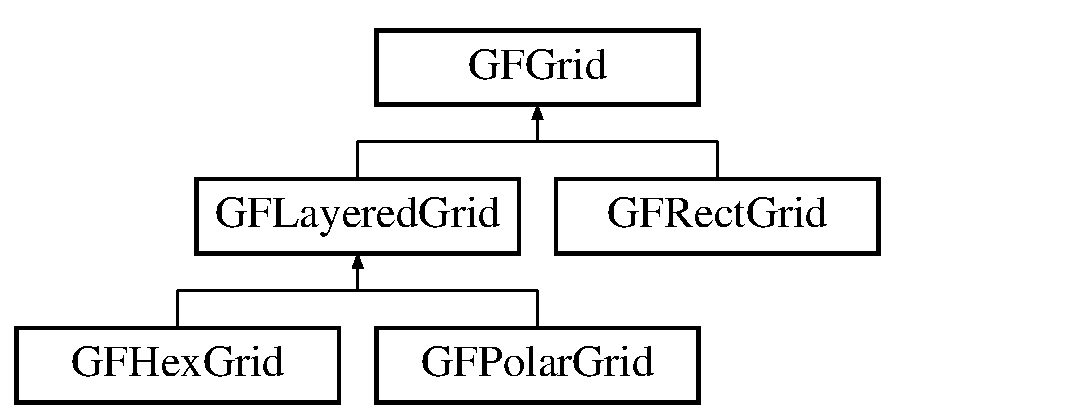
\includegraphics[height=3.000000cm]{class_g_f_grid}
\end{center}
\end{figure}
\subsection*{Public Member Functions}
\begin{DoxyCompactItemize}
\item 
delegate void \hyperlink{class_g_f_grid_a1b011f573c51561fbd9e411f821ba820_a1b011f573c51561fbd9e411f821ba820}{Grid\+Changed\+Delegate} (\hyperlink{class_g_f_grid}{G\+F\+Grid} grid)
\begin{DoxyCompactList}\small\item\em A delegate for handling events when the grid has been changed in such a way that it requires a redraw\end{DoxyCompactList}\item 
abstract Vector3 \hyperlink{class_g_f_grid_a3c424ac71404a8c87a958b5b5952eb0f_a3c424ac71404a8c87a958b5b5952eb0f}{World\+To\+Grid} (Vector3 world\+Point)
\begin{DoxyCompactList}\small\item\em Converts world coordinates to grid coordinates.\end{DoxyCompactList}\item 
abstract Vector3 \hyperlink{class_g_f_grid_af32d7bfcecb5da3fdc47b972b551e33e_af32d7bfcecb5da3fdc47b972b551e33e}{Grid\+To\+World} (Vector3 grid\+Point)
\begin{DoxyCompactList}\small\item\em Converts grid coordinates to world coordinates.\end{DoxyCompactList}\item 
abstract Vector3 \hyperlink{class_g_f_grid_a5865880fa767bf5562301bca419b8bb9_a5865880fa767bf5562301bca419b8bb9}{Nearest\+Vertex\+W} (Vector3 world\+Point, bool do\+Debug)
\begin{DoxyCompactList}\small\item\em Returns the world position of the nearest vertex.\end{DoxyCompactList}\item 
Vector3 \hyperlink{class_g_f_grid_a5a5a2c1544b8f1665cd2ad64e68ad85a_a5a5a2c1544b8f1665cd2ad64e68ad85a}{Nearest\+Vertex\+W} (Vector3 world\+Point)
\item 
abstract Vector3 \hyperlink{class_g_f_grid_ae8711b08c90871f6e88800a30ff5077f_ae8711b08c90871f6e88800a30ff5077f}{Nearest\+Face\+W} (Vector3 world\+Point, \hyperlink{namespace_grid_framework_aa55de93079e09bd55c4cb660025820d5_aa55de93079e09bd55c4cb660025820d5}{Grid\+Plane} plane, bool do\+Debug)
\begin{DoxyCompactList}\small\item\em Returns the world position of the nearest face.\end{DoxyCompactList}\item 
Vector3 \hyperlink{class_g_f_grid_a1f2eb3cedcd2d4f82e23d222136f7743_a1f2eb3cedcd2d4f82e23d222136f7743}{Nearest\+Face\+W} (Vector3 world\+Point, \hyperlink{namespace_grid_framework_aa55de93079e09bd55c4cb660025820d5_aa55de93079e09bd55c4cb660025820d5}{Grid\+Plane} plane)
\item 
abstract Vector3 \hyperlink{class_g_f_grid_a02fcf02269ca5a2064acccecde9819eb_a02fcf02269ca5a2064acccecde9819eb}{Nearest\+Box\+W} (Vector3 world\+Point, bool do\+Debug)
\begin{DoxyCompactList}\small\item\em Returns the world position of the nearest box.\end{DoxyCompactList}\item 
Vector3 \hyperlink{class_g_f_grid_aec31996a483acd023c775658a78d5435_aec31996a483acd023c775658a78d5435}{Nearest\+Box\+W} (Vector3 world\+Point)
\item 
abstract Vector3 \hyperlink{class_g_f_grid_a7eaa2821cf118bb4821bd2cbf40029da_a7eaa2821cf118bb4821bd2cbf40029da}{Nearest\+Vertex\+G} (Vector3 world\+Point)
\begin{DoxyCompactList}\small\item\em Returns the grid position of the nearest vertex.\end{DoxyCompactList}\item 
abstract Vector3 \hyperlink{class_g_f_grid_aac129f3df1da5cdbc31143ecc7db35d2_aac129f3df1da5cdbc31143ecc7db35d2}{Nearest\+Face\+G} (Vector3 world\+Point, \hyperlink{namespace_grid_framework_aa55de93079e09bd55c4cb660025820d5_aa55de93079e09bd55c4cb660025820d5}{Grid\+Plane} plane)
\begin{DoxyCompactList}\small\item\em Returns the grid position of the nearest Face.\end{DoxyCompactList}\item 
abstract Vector3 \hyperlink{class_g_f_grid_adb7c70449b2449c1e82132e6300cc1a5_adb7c70449b2449c1e82132e6300cc1a5}{Nearest\+Box\+G} (Vector3 world\+Point)
\begin{DoxyCompactList}\small\item\em Returns the grid position of the nearest box.\end{DoxyCompactList}\item 
abstract Vector3 \hyperlink{class_g_f_grid_a18b3e57431dc0db8f651479e4fb04a8f_a18b3e57431dc0db8f651479e4fb04a8f}{Align\+Vector3} (Vector3 pos, Vector3 scale, \hyperlink{class_grid_framework_1_1_vectors_1_1_bool_vector3}{Bool\+Vector3} ignore\+Axis)
\begin{DoxyCompactList}\small\item\em Fits a position vector into the grid.\end{DoxyCompactList}\item 
Vector3 \hyperlink{class_g_f_grid_a2c87287a14b02923c9c28aa9d7478eb5_a2c87287a14b02923c9c28aa9d7478eb5}{Align\+Vector3} (Vector3 pos)
\item 
Vector3 \hyperlink{class_g_f_grid_a60adb854cc78a01495dea15affdd158c_a60adb854cc78a01495dea15affdd158c}{Align\+Vector3} (Vector3 pos, \hyperlink{class_grid_framework_1_1_vectors_1_1_bool_vector3}{Bool\+Vector3} lock\+Axis)
\item 
Vector3 \hyperlink{class_g_f_grid_ac08b9392f196d7c87133e343cee64824_ac08b9392f196d7c87133e343cee64824}{Align\+Vector3} (Vector3 pos, Vector3 scale)
\item 
void \hyperlink{class_g_f_grid_ae1005d6635174bc14e02deb4784a8d09_ae1005d6635174bc14e02deb4784a8d09}{Align\+Transform} (Transform the\+Transform, bool rotate, \hyperlink{class_grid_framework_1_1_vectors_1_1_bool_vector3}{Bool\+Vector3} ignore\+Axis)
\begin{DoxyCompactList}\small\item\em Fits a Transform inside the grid (without scaling it).\end{DoxyCompactList}\item 
void \hyperlink{class_g_f_grid_a66b4191eeae96aa23f0ced78f4cc7e14_a66b4191eeae96aa23f0ced78f4cc7e14}{Align\+Transform} (Transform the\+Transform)
\item 
void \hyperlink{class_g_f_grid_a575acf49adeedb3e1cb59108b3c89262_a575acf49adeedb3e1cb59108b3c89262}{Align\+Transform} (Transform the\+Transform, \hyperlink{class_grid_framework_1_1_vectors_1_1_bool_vector3}{Bool\+Vector3} lock\+Axis)
\item 
void \hyperlink{class_g_f_grid_a05a7ee949a05d384656ea1b0befbe485_a05a7ee949a05d384656ea1b0befbe485}{Align\+Transform} (Transform the\+Transform, bool rotate)
\item 
abstract Vector3 \hyperlink{class_g_f_grid_a02b3cf14a1529355c51e0d3ea646b4f8_a02b3cf14a1529355c51e0d3ea646b4f8}{Scale\+Vector3} (Vector3 scl, \hyperlink{class_grid_framework_1_1_vectors_1_1_bool_vector3}{Bool\+Vector3} ignore\+Axis)
\begin{DoxyCompactList}\small\item\em Scales a size vector to fit inside a grid.\end{DoxyCompactList}\item 
Vector3 \hyperlink{class_g_f_grid_a79275b32044dd28cbc80174717390edb_a79275b32044dd28cbc80174717390edb}{Scale\+Vector3} (Vector3 scl)
\item 
void \hyperlink{class_g_f_grid_a20dfd543d80edf6215e7e601cb578ccf_a20dfd543d80edf6215e7e601cb578ccf}{Scale\+Transform} (Transform the\+Transform, \hyperlink{class_grid_framework_1_1_vectors_1_1_bool_vector3}{Bool\+Vector3} ignore\+Axis)
\begin{DoxyCompactList}\small\item\em Scales a Transform to fit the grid (without moving it).\end{DoxyCompactList}\item 
void \hyperlink{class_g_f_grid_a9ad5045b098fde4cea93afeadc1c419d_a9ad5045b098fde4cea93afeadc1c419d}{Scale\+Transform} (Transform the\+Transform)
\item 
void \hyperlink{class_g_f_grid_afe4760ba702ce1e54996f5750501f01f_afe4760ba702ce1e54996f5750501f01f}{Render\+Grid} (Vector3 from, Vector3 to, \hyperlink{class_grid_framework_1_1_vectors_1_1_color_vector3}{Color\+Vector3} colors, int width=0, Camera cam=null, Transform cam\+Transform=null)
\begin{DoxyCompactList}\small\item\em Renders the grid at runtime\end{DoxyCompactList}\item 
virtual void \hyperlink{class_g_f_grid_a24008f73b2c2ce9d6a699d25df998055_a24008f73b2c2ce9d6a699d25df998055}{Render\+Grid} (int width=0, Camera cam=null, Transform cam\+Transform=null)
\item 
void \hyperlink{class_g_f_grid_af700a9a1f9e9f312b1eb55eb8752253c_af700a9a1f9e9f312b1eb55eb8752253c}{Render\+Grid} (Vector3 from, Vector3 to, int width=0, Camera cam=null, Transform cam\+Transform=null)
\item 
void \hyperlink{class_g_f_grid_a150a203272b059999baa0eb3b8a74b09_a150a203272b059999baa0eb3b8a74b09}{Draw\+Grid} (Vector3 from, Vector3 to)
\begin{DoxyCompactList}\small\item\em Draws the grid using gizmos.\end{DoxyCompactList}\item 
void \hyperlink{class_g_f_grid_ae151fe7e54efa0fedaa5e67da1077682_ae151fe7e54efa0fedaa5e67da1077682}{Draw\+Grid} ()
\item 
Vector3\mbox{[}$\,$\mbox{]} \hyperlink{class_g_f_grid_a21a5ed4cfa330e04e6ce8c951744b839_a21a5ed4cfa330e04e6ce8c951744b839}{Get\+Vectrosity\+Points} (Vector3 from, Vector3 to)
\begin{DoxyCompactList}\small\item\em Returns an array of Vector3 points ready for use with Vectrosity.\end{DoxyCompactList}\item 
Vector3\mbox{[}$\,$\mbox{]} \hyperlink{class_g_f_grid_a8ee183793ee692d671e39aaa93f4928e_a8ee183793ee692d671e39aaa93f4928e}{Get\+Vectrosity\+Points} ()
\item 
Vector3\mbox{[}$\,$\mbox{]}\mbox{[}$\,$\mbox{]} \hyperlink{class_g_f_grid_a53cd898dc26179856ac298b5213e6dfb_a53cd898dc26179856ac298b5213e6dfb}{Get\+Vectrosity\+Points\+Separate} (Vector3 from, Vector3 to)
\begin{DoxyCompactList}\small\item\em Returns an array of arrays of Vector3 points ready for use with Vectrosity.\end{DoxyCompactList}\item 
Vector3\mbox{[}$\,$\mbox{]}\mbox{[}$\,$\mbox{]} \hyperlink{class_g_f_grid_a9c0d4962f326ba00115a40a2b82d0aa7_a9c0d4962f326ba00115a40a2b82d0aa7}{Get\+Vectrosity\+Points\+Separate} ()
\end{DoxyCompactItemize}
\subsection*{Public Attributes}
\begin{DoxyCompactItemize}
\item 
\hyperlink{class_grid_framework_1_1_vectors_1_1_color_vector3}{Color\+Vector3} \hyperlink{class_g_f_grid_aa0dc7222dee5910e8df47e133f719309_aa0dc7222dee5910e8df47e133f719309}{axis\+Colors} = new \hyperlink{class_grid_framework_1_1_vectors_1_1_color_vector3}{Color\+Vector3}()
\begin{DoxyCompactList}\small\item\em Colours of the axes when drawing and rendering.\end{DoxyCompactList}\item 
bool \hyperlink{class_g_f_grid_aeb78dcbc2890d20556958c994b95b000_aeb78dcbc2890d20556958c994b95b000}{use\+Separate\+Render\+Color} = false
\begin{DoxyCompactList}\small\item\em Whether to use the same colours for rendering as for drawing.\end{DoxyCompactList}\item 
\hyperlink{class_grid_framework_1_1_vectors_1_1_color_vector3}{Color\+Vector3} \hyperlink{class_g_f_grid_a8a822dbae0fa74657a7beed9761a0e89_a8a822dbae0fa74657a7beed9761a0e89}{render\+Axis\+Colors} = new \hyperlink{class_grid_framework_1_1_vectors_1_1_color_vector3}{Color\+Vector3}(Color.\+gray)
\begin{DoxyCompactList}\small\item\em Separate colours of the axes when rendering.\end{DoxyCompactList}\item 
bool \hyperlink{class_g_f_grid_afa8a9e01aac581a365606ac8c1b4af64_afa8a9e01aac581a365606ac8c1b4af64}{hide\+Grid} = false
\begin{DoxyCompactList}\small\item\em Whether to hide the grid completely.\end{DoxyCompactList}\item 
bool \hyperlink{class_g_f_grid_a9a57a01347c8ab0a6401aa210f875ab0_a9a57a01347c8ab0a6401aa210f875ab0}{hide\+On\+Play} = false
\begin{DoxyCompactList}\small\item\em Whether to hide the grid in play mode.\end{DoxyCompactList}\item 
\hyperlink{class_grid_framework_1_1_vectors_1_1_bool_vector3}{Bool\+Vector3} \hyperlink{class_g_f_grid_ac902d0ffe9b552908a929fda497a39b5_ac902d0ffe9b552908a929fda497a39b5}{hide\+Axis} = new \hyperlink{class_grid_framework_1_1_vectors_1_1_bool_vector3}{Bool\+Vector3}()
\begin{DoxyCompactList}\small\item\em Whether to hide just individual axes.\end{DoxyCompactList}\item 
bool \hyperlink{class_g_f_grid_a030e49e310751d9b1c7d08b57ca93358_a030e49e310751d9b1c7d08b57ca93358}{draw\+Origin} = false
\begin{DoxyCompactList}\small\item\em Whether to draw a little sphere at the origin of the grid.\end{DoxyCompactList}\item 
bool \hyperlink{class_g_f_grid_a8b33c2e0823730157804456f4ffb51ed_a8b33c2e0823730157804456f4ffb51ed}{render\+Grid} = true
\begin{DoxyCompactList}\small\item\em Whether to render the grid at runtime.\end{DoxyCompactList}\item 
Material \hyperlink{class_g_f_grid_a5a840197e72fa8b32fb905cc2a9a4d4a_a5a840197e72fa8b32fb905cc2a9a4d4a}{render\+Material} = null
\begin{DoxyCompactList}\small\item\em The material for rendering, if none is given it uses a default material.\end{DoxyCompactList}\end{DoxyCompactItemize}
\subsection*{Properties}
\begin{DoxyCompactItemize}
\item 
bool \hyperlink{class_g_f_grid_a65d207e3957240c935645db01a199419_a65d207e3957240c935645db01a199419}{relative\+Size}\hspace{0.3cm}{\ttfamily  \mbox{[}get, set\mbox{]}}
\begin{DoxyCompactList}\small\item\em Whether the drawing/rendering will scale with spacing.\end{DoxyCompactList}\item 
virtual Vector3 \hyperlink{class_g_f_grid_a336f54e5b5f677871876dc3d90cc611d_a336f54e5b5f677871876dc3d90cc611d}{size}\hspace{0.3cm}{\ttfamily  \mbox{[}get, set\mbox{]}}
\begin{DoxyCompactList}\small\item\em The size of the visual representation of the grid.\end{DoxyCompactList}\item 
virtual Vector3 \hyperlink{class_g_f_grid_a4556eac3905975b9024addb169c629d8_a4556eac3905975b9024addb169c629d8}{render\+From}\hspace{0.3cm}{\ttfamily  \mbox{[}get, set\mbox{]}}
\begin{DoxyCompactList}\small\item\em Custom lower limit for drawing and rendering.\end{DoxyCompactList}\item 
virtual Vector3 \hyperlink{class_g_f_grid_af9ec4b040505718f58a7841087d9b72a_af9ec4b040505718f58a7841087d9b72a}{render\+To}\hspace{0.3cm}{\ttfamily  \mbox{[}get, set\mbox{]}}
\begin{DoxyCompactList}\small\item\em Custom upper limit for drawing and rendering.\end{DoxyCompactList}\item 
Vector3 \hyperlink{class_g_f_grid_a6fb374bcb7d726ff28e3f14817260d6c_a6fb374bcb7d726ff28e3f14817260d6c}{origin\+Offset}\hspace{0.3cm}{\ttfamily  \mbox{[}get, set\mbox{]}}
\begin{DoxyCompactList}\small\item\em Offset to add to the origin\end{DoxyCompactList}\item 
bool \hyperlink{class_g_f_grid_acb950aa31097c85e153cd9a642900a31_acb950aa31097c85e153cd9a642900a31}{use\+Custom\+Render\+Range}\hspace{0.3cm}{\ttfamily  \mbox{[}get, set\mbox{]}}
\begin{DoxyCompactList}\small\item\em Use your own values for the range of the rendering.\end{DoxyCompactList}\item 
int \hyperlink{class_g_f_grid_a6712a2e6fec379ea55a0a53ca5867216_a6712a2e6fec379ea55a0a53ca5867216}{render\+Line\+Width}\hspace{0.3cm}{\ttfamily  \mbox{[}get, set\mbox{]}}
\begin{DoxyCompactList}\small\item\em The width of the lines used when rendering the grid.\end{DoxyCompactList}\end{DoxyCompactItemize}
\subsection*{Events}
\begin{DoxyCompactItemize}
\item 
\hyperlink{class_g_f_grid_a1b011f573c51561fbd9e411f821ba820_a1b011f573c51561fbd9e411f821ba820}{Grid\+Changed\+Delegate} \hyperlink{class_g_f_grid_af3bfbed41ba24f963e871921c663f1f8_af3bfbed41ba24f963e871921c663f1f8}{Grid\+Changed\+Event}
\begin{DoxyCompactList}\small\item\em An even that gets fired \end{DoxyCompactList}\end{DoxyCompactItemize}


\subsection{Detailed Description}
This is the standard class all grids are based on. Aside from providing a common set of variables and a template for what methods to use, this class has no practical meaning for end users. Use this as reference for what can be done without having to specify which type of grid you are using. For anything more specific you have to look at the child classes. 

\subsection{Member Function Documentation}
\hypertarget{class_g_f_grid_ae1005d6635174bc14e02deb4784a8d09_ae1005d6635174bc14e02deb4784a8d09}{\index{G\+F\+Grid@{G\+F\+Grid}!Align\+Transform@{Align\+Transform}}
\index{Align\+Transform@{Align\+Transform}!G\+F\+Grid@{G\+F\+Grid}}
\subsubsection[{Align\+Transform}]{\setlength{\rightskip}{0pt plus 5cm}void G\+F\+Grid.\+Align\+Transform (
\begin{DoxyParamCaption}
\item[{Transform}]{the\+Transform, }
\item[{bool}]{rotate, }
\item[{{\bf Bool\+Vector3}}]{ignore\+Axis}
\end{DoxyParamCaption}
)}}\label{class_g_f_grid_ae1005d6635174bc14e02deb4784a8d09_ae1005d6635174bc14e02deb4784a8d09}

\begin{DoxyParams}{Parameters}
{\em the\+Transform} & The Transform to align.\\
\hline
{\em rotate} & Whether to rotate to the grid.\\
\hline
{\em ignore\+Axis} & Which axes should be ignored.\\
\hline
\end{DoxyParams}


Fits an object inside the grid by using the object’s Transform. Setting {\ttfamily do\+Rotate} makes the object take on the grid’s rotation. The parameter {\ttfamily lock\+Axis} makes the function not touch the corresponding coordinate.

The resulting position depends on {\itshape Align\+Vector3} , so please look up how that method works. \hypertarget{class_g_f_grid_a66b4191eeae96aa23f0ced78f4cc7e14_a66b4191eeae96aa23f0ced78f4cc7e14}{\index{G\+F\+Grid@{G\+F\+Grid}!Align\+Transform@{Align\+Transform}}
\index{Align\+Transform@{Align\+Transform}!G\+F\+Grid@{G\+F\+Grid}}
\subsubsection[{Align\+Transform}]{\setlength{\rightskip}{0pt plus 5cm}void G\+F\+Grid.\+Align\+Transform (
\begin{DoxyParamCaption}
\item[{Transform}]{the\+Transform}
\end{DoxyParamCaption}
)}}\label{class_g_f_grid_a66b4191eeae96aa23f0ced78f4cc7e14_a66b4191eeae96aa23f0ced78f4cc7e14}
This is an overloaded member function, provided for convenience. It differs from the above function only in what argument(s) it accepts. It aligns and rotates the Transform while respecting all axes, it is equal to {\ttfamily Align\+Transform(the\+Transform, true, new Bool\+Vector3(false));} \hypertarget{class_g_f_grid_a575acf49adeedb3e1cb59108b3c89262_a575acf49adeedb3e1cb59108b3c89262}{\index{G\+F\+Grid@{G\+F\+Grid}!Align\+Transform@{Align\+Transform}}
\index{Align\+Transform@{Align\+Transform}!G\+F\+Grid@{G\+F\+Grid}}
\subsubsection[{Align\+Transform}]{\setlength{\rightskip}{0pt plus 5cm}void G\+F\+Grid.\+Align\+Transform (
\begin{DoxyParamCaption}
\item[{Transform}]{the\+Transform, }
\item[{{\bf Bool\+Vector3}}]{lock\+Axis}
\end{DoxyParamCaption}
)}}\label{class_g_f_grid_a575acf49adeedb3e1cb59108b3c89262_a575acf49adeedb3e1cb59108b3c89262}
This is an overloaded member function, provided for convenience. It differs from the above function only in what argument(s) it accepts. It aligns and rotates the Transform but leaves the axes to the user, it is equal to {\ttfamily Align\+Transform(the\+Transform, true, lock\+Axis);} \hypertarget{class_g_f_grid_a05a7ee949a05d384656ea1b0befbe485_a05a7ee949a05d384656ea1b0befbe485}{\index{G\+F\+Grid@{G\+F\+Grid}!Align\+Transform@{Align\+Transform}}
\index{Align\+Transform@{Align\+Transform}!G\+F\+Grid@{G\+F\+Grid}}
\subsubsection[{Align\+Transform}]{\setlength{\rightskip}{0pt plus 5cm}void G\+F\+Grid.\+Align\+Transform (
\begin{DoxyParamCaption}
\item[{Transform}]{the\+Transform, }
\item[{bool}]{rotate}
\end{DoxyParamCaption}
)}}\label{class_g_f_grid_a05a7ee949a05d384656ea1b0befbe485_a05a7ee949a05d384656ea1b0befbe485}
This is an overloaded member function, provided for convenience. It differs from the above function only in what argument(s) it accepts. It aligns and respects all axes to the user, but leaves the decision of rotation to the user, it is equal to {\ttfamily Align\+Transform(the\+Transform, rotate, new Bool\+Vector3(false));} \hypertarget{class_g_f_grid_a18b3e57431dc0db8f651479e4fb04a8f_a18b3e57431dc0db8f651479e4fb04a8f}{\index{G\+F\+Grid@{G\+F\+Grid}!Align\+Vector3@{Align\+Vector3}}
\index{Align\+Vector3@{Align\+Vector3}!G\+F\+Grid@{G\+F\+Grid}}
\subsubsection[{Align\+Vector3}]{\setlength{\rightskip}{0pt plus 5cm}abstract Vector3 G\+F\+Grid.\+Align\+Vector3 (
\begin{DoxyParamCaption}
\item[{Vector3}]{pos, }
\item[{Vector3}]{scale, }
\item[{{\bf Bool\+Vector3}}]{ignore\+Axis}
\end{DoxyParamCaption}
)\hspace{0.3cm}{\ttfamily [pure virtual]}}}\label{class_g_f_grid_a18b3e57431dc0db8f651479e4fb04a8f_a18b3e57431dc0db8f651479e4fb04a8f}
\begin{DoxyReturn}{Returns}
Aligned position vector.
\end{DoxyReturn}

\begin{DoxyParams}{Parameters}
{\em pos} & The position to align.\\
\hline
{\em scale} & A simulated scale to decide how exactly to fit the poistion into the grid.\\
\hline
{\em ignore\+Axis} & Which axes should be ignored.\\
\hline
\end{DoxyParams}


Fits a position inside the grid by using the object’s transform. The exact position depends on whether the components of {\itshape scale}  are even or odd and the exact implementation can be found in the subclasses. The parameter {\itshape ignore\+Axis}  makes the function not touch the corresponding coordinate. 

Implemented in \hyperlink{class_g_f_hex_grid_a2d51f41dc859b4957bb67a518c252632_a2d51f41dc859b4957bb67a518c252632}{G\+F\+Hex\+Grid}, \hyperlink{class_g_f_polar_grid_a5faa2b607e1ffc4ad2d3d5e7d62bf611_a5faa2b607e1ffc4ad2d3d5e7d62bf611}{G\+F\+Polar\+Grid}, and \hyperlink{class_g_f_rect_grid_a26011b42493622436cd9a86516b82687_a26011b42493622436cd9a86516b82687}{G\+F\+Rect\+Grid}.

\hypertarget{class_g_f_grid_a2c87287a14b02923c9c28aa9d7478eb5_a2c87287a14b02923c9c28aa9d7478eb5}{\index{G\+F\+Grid@{G\+F\+Grid}!Align\+Vector3@{Align\+Vector3}}
\index{Align\+Vector3@{Align\+Vector3}!G\+F\+Grid@{G\+F\+Grid}}
\subsubsection[{Align\+Vector3}]{\setlength{\rightskip}{0pt plus 5cm}Vector3 G\+F\+Grid.\+Align\+Vector3 (
\begin{DoxyParamCaption}
\item[{Vector3}]{pos}
\end{DoxyParamCaption}
)}}\label{class_g_f_grid_a2c87287a14b02923c9c28aa9d7478eb5_a2c87287a14b02923c9c28aa9d7478eb5}
This is an overloaded member function, provided for convenience. It differs from the above function only in what argument(s) it accepts. It aligns the position while respecting all axes and uses a default size of 1 x 1 x 1, it is equal to {\ttfamily Align\+Vector3(pos, Vector3.\+one, new Bool\+Vector3(false));} \hypertarget{class_g_f_grid_a60adb854cc78a01495dea15affdd158c_a60adb854cc78a01495dea15affdd158c}{\index{G\+F\+Grid@{G\+F\+Grid}!Align\+Vector3@{Align\+Vector3}}
\index{Align\+Vector3@{Align\+Vector3}!G\+F\+Grid@{G\+F\+Grid}}
\subsubsection[{Align\+Vector3}]{\setlength{\rightskip}{0pt plus 5cm}Vector3 G\+F\+Grid.\+Align\+Vector3 (
\begin{DoxyParamCaption}
\item[{Vector3}]{pos, }
\item[{{\bf Bool\+Vector3}}]{lock\+Axis}
\end{DoxyParamCaption}
)}}\label{class_g_f_grid_a60adb854cc78a01495dea15affdd158c_a60adb854cc78a01495dea15affdd158c}
This is an overloaded member function, provided for convenience. It differs from the above function only in what argument(s) it accepts. It aligns the position and uses a default size of 1 x 1 x 1 while leaving the axes to the user, it is equal to {\ttfamily Align\+Vector3(pos, Vector3.\+one, lock\+Axis);} \hypertarget{class_g_f_grid_ac08b9392f196d7c87133e343cee64824_ac08b9392f196d7c87133e343cee64824}{\index{G\+F\+Grid@{G\+F\+Grid}!Align\+Vector3@{Align\+Vector3}}
\index{Align\+Vector3@{Align\+Vector3}!G\+F\+Grid@{G\+F\+Grid}}
\subsubsection[{Align\+Vector3}]{\setlength{\rightskip}{0pt plus 5cm}Vector3 G\+F\+Grid.\+Align\+Vector3 (
\begin{DoxyParamCaption}
\item[{Vector3}]{pos, }
\item[{Vector3}]{scale}
\end{DoxyParamCaption}
)}}\label{class_g_f_grid_ac08b9392f196d7c87133e343cee64824_ac08b9392f196d7c87133e343cee64824}
This is an overloaded member function, provided for convenience. It differs from the above function only in what argument(s) it accepts. It aligns the position and respects the axes while using a default size of 1 x 1 x 1, it is equal to {\ttfamily Align\+Vector3(pos, scale, new Bool\+Vector3(false));} \hypertarget{class_g_f_grid_a150a203272b059999baa0eb3b8a74b09_a150a203272b059999baa0eb3b8a74b09}{\index{G\+F\+Grid@{G\+F\+Grid}!Draw\+Grid@{Draw\+Grid}}
\index{Draw\+Grid@{Draw\+Grid}!G\+F\+Grid@{G\+F\+Grid}}
\subsubsection[{Draw\+Grid}]{\setlength{\rightskip}{0pt plus 5cm}void G\+F\+Grid.\+Draw\+Grid (
\begin{DoxyParamCaption}
\item[{Vector3}]{from, }
\item[{Vector3}]{to}
\end{DoxyParamCaption}
)}}\label{class_g_f_grid_a150a203272b059999baa0eb3b8a74b09_a150a203272b059999baa0eb3b8a74b09}

\begin{DoxyParams}{Parameters}
{\em from} & Lower limit of the drawing.\\
\hline
{\em to} & Upper limit s drawing.\\
\hline
\end{DoxyParams}


This method draws the grid in the editor using gizmos. There is usually no reason to call this method manually, you should instead set the drawing flags of the grid itself. However, if you must, call this method from inside {\ttfamily \href{http://docs.unity3d.com/Documentation/ScriptReference/MonoBehaviour.OnDrawGizmos.html}{\tt On\+Draw\+Gizmos}}. \hypertarget{class_g_f_grid_ae151fe7e54efa0fedaa5e67da1077682_ae151fe7e54efa0fedaa5e67da1077682}{\index{G\+F\+Grid@{G\+F\+Grid}!Draw\+Grid@{Draw\+Grid}}
\index{Draw\+Grid@{Draw\+Grid}!G\+F\+Grid@{G\+F\+Grid}}
\subsubsection[{Draw\+Grid}]{\setlength{\rightskip}{0pt plus 5cm}void G\+F\+Grid.\+Draw\+Grid (
\begin{DoxyParamCaption}
{}
\end{DoxyParamCaption}
)}}\label{class_g_f_grid_ae151fe7e54efa0fedaa5e67da1077682_ae151fe7e54efa0fedaa5e67da1077682}
This is an overloaded member function, provided for convenience. It differs from the above function only in what argument(s) it accepts. Uses the size as limits, it is equivalent to {\ttfamily Draw\+Grid(-\/size, size);} \hypertarget{class_g_f_grid_a21a5ed4cfa330e04e6ce8c951744b839_a21a5ed4cfa330e04e6ce8c951744b839}{\index{G\+F\+Grid@{G\+F\+Grid}!Get\+Vectrosity\+Points@{Get\+Vectrosity\+Points}}
\index{Get\+Vectrosity\+Points@{Get\+Vectrosity\+Points}!G\+F\+Grid@{G\+F\+Grid}}
\subsubsection[{Get\+Vectrosity\+Points}]{\setlength{\rightskip}{0pt plus 5cm}Vector3 \mbox{[}$\,$\mbox{]} G\+F\+Grid.\+Get\+Vectrosity\+Points (
\begin{DoxyParamCaption}
\item[{Vector3}]{from, }
\item[{Vector3}]{to}
\end{DoxyParamCaption}
)}}\label{class_g_f_grid_a21a5ed4cfa330e04e6ce8c951744b839_a21a5ed4cfa330e04e6ce8c951744b839}
\begin{DoxyReturn}{Returns}
Array of points in local space.
\end{DoxyReturn}

\begin{DoxyParams}{Parameters}
{\em from} & Lower limit for the points.\\
\hline
{\em to} & Upper limit for the points.\\
\hline
\end{DoxyParams}


Returns an array of Vector3 containing the points for a discrete vector line in Vectrosity. One entry is the starting point, the next entry is the end point, the next entry is the starting point of the next line and so on. \hypertarget{class_g_f_grid_a8ee183793ee692d671e39aaa93f4928e_a8ee183793ee692d671e39aaa93f4928e}{\index{G\+F\+Grid@{G\+F\+Grid}!Get\+Vectrosity\+Points@{Get\+Vectrosity\+Points}}
\index{Get\+Vectrosity\+Points@{Get\+Vectrosity\+Points}!G\+F\+Grid@{G\+F\+Grid}}
\subsubsection[{Get\+Vectrosity\+Points}]{\setlength{\rightskip}{0pt plus 5cm}Vector3 \mbox{[}$\,$\mbox{]} G\+F\+Grid.\+Get\+Vectrosity\+Points (
\begin{DoxyParamCaption}
{}
\end{DoxyParamCaption}
)}}\label{class_g_f_grid_a8ee183793ee692d671e39aaa93f4928e_a8ee183793ee692d671e39aaa93f4928e}
This is an overloaded member function, provided for convenience. It differs from the above function only in what argument(s) it accepts. Uses the grid's {\ttfamily \hyperlink{class_g_f_grid_a336f54e5b5f677871876dc3d90cc611d_a336f54e5b5f677871876dc3d90cc611d}{size}} or {\ttfamily \hyperlink{class_g_f_grid_a4556eac3905975b9024addb169c629d8_a4556eac3905975b9024addb169c629d8}{render\+From}} and {\ttfamily \hyperlink{class_g_f_grid_af9ec4b040505718f58a7841087d9b72a_af9ec4b040505718f58a7841087d9b72a}{render\+To}} as limits, equal to {\ttfamily use\+Custom\+Render\+Range ? Get\+Vectrosity\+Points(render\+From, render\+To) \+: Get\+Vectrosity\+Points(-\/size, size);} \hypertarget{class_g_f_grid_a53cd898dc26179856ac298b5213e6dfb_a53cd898dc26179856ac298b5213e6dfb}{\index{G\+F\+Grid@{G\+F\+Grid}!Get\+Vectrosity\+Points\+Separate@{Get\+Vectrosity\+Points\+Separate}}
\index{Get\+Vectrosity\+Points\+Separate@{Get\+Vectrosity\+Points\+Separate}!G\+F\+Grid@{G\+F\+Grid}}
\subsubsection[{Get\+Vectrosity\+Points\+Separate}]{\setlength{\rightskip}{0pt plus 5cm}Vector3 \mbox{[}$\,$\mbox{]}\mbox{[}$\,$\mbox{]} G\+F\+Grid.\+Get\+Vectrosity\+Points\+Separate (
\begin{DoxyParamCaption}
\item[{Vector3}]{from, }
\item[{Vector3}]{to}
\end{DoxyParamCaption}
)}}\label{class_g_f_grid_a53cd898dc26179856ac298b5213e6dfb_a53cd898dc26179856ac298b5213e6dfb}
\begin{DoxyReturn}{Returns}
Jagged array of three arrays, each containing the points of a single axis.
\end{DoxyReturn}

\begin{DoxyParams}{Parameters}
{\em from} & Lower limit for the points.\\
\hline
{\em to} & Upper limit for the points.\\
\hline
\end{DoxyParams}


This method is very similar to {\ttfamily \hyperlink{class_g_f_grid_a21a5ed4cfa330e04e6ce8c951744b839_a21a5ed4cfa330e04e6ce8c951744b839}{Get\+Vectrosity\+Points}}, except that the points are in separate arrays for each axis. This is useful if you want to treat the lines of each axis differently, like having different colours. \hypertarget{class_g_f_grid_a9c0d4962f326ba00115a40a2b82d0aa7_a9c0d4962f326ba00115a40a2b82d0aa7}{\index{G\+F\+Grid@{G\+F\+Grid}!Get\+Vectrosity\+Points\+Separate@{Get\+Vectrosity\+Points\+Separate}}
\index{Get\+Vectrosity\+Points\+Separate@{Get\+Vectrosity\+Points\+Separate}!G\+F\+Grid@{G\+F\+Grid}}
\subsubsection[{Get\+Vectrosity\+Points\+Separate}]{\setlength{\rightskip}{0pt plus 5cm}Vector3 \mbox{[}$\,$\mbox{]}\mbox{[}$\,$\mbox{]} G\+F\+Grid.\+Get\+Vectrosity\+Points\+Separate (
\begin{DoxyParamCaption}
{}
\end{DoxyParamCaption}
)}}\label{class_g_f_grid_a9c0d4962f326ba00115a40a2b82d0aa7_a9c0d4962f326ba00115a40a2b82d0aa7}
This is an overloaded member function, provided for convenience. It differs from the above function only in what argument(s) it accepts. Uses the grid's {\ttfamily \hyperlink{class_g_f_grid_a336f54e5b5f677871876dc3d90cc611d_a336f54e5b5f677871876dc3d90cc611d}{size}} or {\ttfamily \hyperlink{class_g_f_grid_a4556eac3905975b9024addb169c629d8_a4556eac3905975b9024addb169c629d8}{render\+From}} and {\ttfamily \hyperlink{class_g_f_grid_af9ec4b040505718f58a7841087d9b72a_af9ec4b040505718f58a7841087d9b72a}{render\+To}} as limits, equal to {\ttfamily use\+Custom\+Render\+Range ? Get\+Vectrosity\+Points\+Separate(render\+From, render\+To) \+: Get\+Vectrosity\+Points\+Separate(-\/size, size);} \hypertarget{class_g_f_grid_a1b011f573c51561fbd9e411f821ba820_a1b011f573c51561fbd9e411f821ba820}{\index{G\+F\+Grid@{G\+F\+Grid}!Grid\+Changed\+Delegate@{Grid\+Changed\+Delegate}}
\index{Grid\+Changed\+Delegate@{Grid\+Changed\+Delegate}!G\+F\+Grid@{G\+F\+Grid}}
\subsubsection[{Grid\+Changed\+Delegate}]{\setlength{\rightskip}{0pt plus 5cm}delegate void G\+F\+Grid.\+Grid\+Changed\+Delegate (
\begin{DoxyParamCaption}
\item[{{\bf G\+F\+Grid}}]{grid}
\end{DoxyParamCaption}
)}}\label{class_g_f_grid_a1b011f573c51561fbd9e411f821ba820_a1b011f573c51561fbd9e411f821ba820}

\begin{DoxyParams}{Parameters}
{\em grid} & The grid that calls the delegate\\
\hline
\end{DoxyParams}


This is the delegate type for methods to be called when changes to the grid occur. It is best used together with the \hyperlink{class_g_f_grid_af3bfbed41ba24f963e871921c663f1f8_af3bfbed41ba24f963e871921c663f1f8}{Grid\+Changed\+Event} event. \hypertarget{class_g_f_grid_af32d7bfcecb5da3fdc47b972b551e33e_af32d7bfcecb5da3fdc47b972b551e33e}{\index{G\+F\+Grid@{G\+F\+Grid}!Grid\+To\+World@{Grid\+To\+World}}
\index{Grid\+To\+World@{Grid\+To\+World}!G\+F\+Grid@{G\+F\+Grid}}
\subsubsection[{Grid\+To\+World}]{\setlength{\rightskip}{0pt plus 5cm}abstract Vector3 G\+F\+Grid.\+Grid\+To\+World (
\begin{DoxyParamCaption}
\item[{Vector3}]{grid\+Point}
\end{DoxyParamCaption}
)\hspace{0.3cm}{\ttfamily [pure virtual]}}}\label{class_g_f_grid_af32d7bfcecb5da3fdc47b972b551e33e_af32d7bfcecb5da3fdc47b972b551e33e}
\begin{DoxyReturn}{Returns}
World coordinates of the grid point.
\end{DoxyReturn}

\begin{DoxyParams}{Parameters}
{\em grid\+Point} & Point in grid space.\\
\hline
\end{DoxyParams}


Takes in a point in grid space and converts it to world space. Some grids have several coordinate system, so look into the specific class for conversion methods from other coordinate systems. 

Implemented in \hyperlink{class_g_f_hex_grid_abac4ca6dba9e7ee8ed87f70cf4a7afc7_abac4ca6dba9e7ee8ed87f70cf4a7afc7}{G\+F\+Hex\+Grid}, \hyperlink{class_g_f_polar_grid_a80a4698250b08f212f3681abadbc5012_a80a4698250b08f212f3681abadbc5012}{G\+F\+Polar\+Grid}, and \hyperlink{class_g_f_rect_grid_acdc111b97728b0fef0c32e2d96d59f90_acdc111b97728b0fef0c32e2d96d59f90}{G\+F\+Rect\+Grid}.

\hypertarget{class_g_f_grid_adb7c70449b2449c1e82132e6300cc1a5_adb7c70449b2449c1e82132e6300cc1a5}{\index{G\+F\+Grid@{G\+F\+Grid}!Nearest\+Box\+G@{Nearest\+Box\+G}}
\index{Nearest\+Box\+G@{Nearest\+Box\+G}!G\+F\+Grid@{G\+F\+Grid}}
\subsubsection[{Nearest\+Box\+G}]{\setlength{\rightskip}{0pt plus 5cm}abstract Vector3 G\+F\+Grid.\+Nearest\+Box\+G (
\begin{DoxyParamCaption}
\item[{Vector3}]{world\+Point}
\end{DoxyParamCaption}
)\hspace{0.3cm}{\ttfamily [pure virtual]}}}\label{class_g_f_grid_adb7c70449b2449c1e82132e6300cc1a5_adb7c70449b2449c1e82132e6300cc1a5}
\begin{DoxyReturn}{Returns}
Grid position of the nearest box.
\end{DoxyReturn}

\begin{DoxyParams}{Parameters}
{\em world\+Point} & Point in world space.\\
\hline
\end{DoxyParams}


Similar to \hyperlink{class_g_f_grid_a7eaa2821cf118bb4821bd2cbf40029da_a7eaa2821cf118bb4821bd2cbf40029da}{Nearest\+Vertex\+G}, it returns the grid coordinates of a box in the grid. Since the box is enclosed by several vertices, the returned value is the point in between all of the vertices.

This is just an abstract template for the method, look into the specific class for exact implementation. 

Implemented in \hyperlink{class_g_f_hex_grid_ab038b99bc1bedfcdee8a0736c4ed1a1e_ab038b99bc1bedfcdee8a0736c4ed1a1e}{G\+F\+Hex\+Grid}, \hyperlink{class_g_f_polar_grid_abdc5c38b32d8fe3d6610127b54b89093_abdc5c38b32d8fe3d6610127b54b89093}{G\+F\+Polar\+Grid}, and \hyperlink{class_g_f_rect_grid_a97bcb6df6296fac0bcf92c9d8908df00_a97bcb6df6296fac0bcf92c9d8908df00}{G\+F\+Rect\+Grid}.

\hypertarget{class_g_f_grid_a02fcf02269ca5a2064acccecde9819eb_a02fcf02269ca5a2064acccecde9819eb}{\index{G\+F\+Grid@{G\+F\+Grid}!Nearest\+Box\+W@{Nearest\+Box\+W}}
\index{Nearest\+Box\+W@{Nearest\+Box\+W}!G\+F\+Grid@{G\+F\+Grid}}
\subsubsection[{Nearest\+Box\+W}]{\setlength{\rightskip}{0pt plus 5cm}abstract Vector3 G\+F\+Grid.\+Nearest\+Box\+W (
\begin{DoxyParamCaption}
\item[{Vector3}]{world\+Point, }
\item[{bool}]{do\+Debug}
\end{DoxyParamCaption}
)\hspace{0.3cm}{\ttfamily [pure virtual]}}}\label{class_g_f_grid_a02fcf02269ca5a2064acccecde9819eb_a02fcf02269ca5a2064acccecde9819eb}
\begin{DoxyReturn}{Returns}
World position of the nearest box.
\end{DoxyReturn}

\begin{DoxyParams}{Parameters}
{\em world\+Point} & Point in world space.\\
\hline
{\em do\+Debug} & If set to {\ttfamily true} draw a sphere at the destination.\\
\hline
\end{DoxyParams}


Similar to \hyperlink{class_g_f_grid_a5865880fa767bf5562301bca419b8bb9_a5865880fa767bf5562301bca419b8bb9}{Nearest\+Vertex\+W}, it returns the world coordinates of a box in the grid. Since the box is enclosed by several vertices, the returned value is the point in between all of the vertices. If {\itshape do\+Debug}  is set a small gizmo box will drawn there.

This is just an abstract template for the method, look into the specific class for exact implementation. 

Implemented in \hyperlink{class_g_f_hex_grid_a58ce4a0c91753d5457c4df0ebaac90a9_a58ce4a0c91753d5457c4df0ebaac90a9}{G\+F\+Hex\+Grid}, \hyperlink{class_g_f_polar_grid_aa8d60db8cd64b7dbe083d380110ab9d9_aa8d60db8cd64b7dbe083d380110ab9d9}{G\+F\+Polar\+Grid}, and \hyperlink{class_g_f_rect_grid_a36755945173349f1d24c3a41092bc6f4_a36755945173349f1d24c3a41092bc6f4}{G\+F\+Rect\+Grid}.

\hypertarget{class_g_f_grid_aec31996a483acd023c775658a78d5435_aec31996a483acd023c775658a78d5435}{\index{G\+F\+Grid@{G\+F\+Grid}!Nearest\+Box\+W@{Nearest\+Box\+W}}
\index{Nearest\+Box\+W@{Nearest\+Box\+W}!G\+F\+Grid@{G\+F\+Grid}}
\subsubsection[{Nearest\+Box\+W}]{\setlength{\rightskip}{0pt plus 5cm}Vector3 G\+F\+Grid.\+Nearest\+Box\+W (
\begin{DoxyParamCaption}
\item[{Vector3}]{world\+Point}
\end{DoxyParamCaption}
)}}\label{class_g_f_grid_aec31996a483acd023c775658a78d5435_aec31996a483acd023c775658a78d5435}
This is an overloaded member function, provided for convenience. It differs from the above function only in what argument(s) it accepts. \hypertarget{class_g_f_grid_aac129f3df1da5cdbc31143ecc7db35d2_aac129f3df1da5cdbc31143ecc7db35d2}{\index{G\+F\+Grid@{G\+F\+Grid}!Nearest\+Face\+G@{Nearest\+Face\+G}}
\index{Nearest\+Face\+G@{Nearest\+Face\+G}!G\+F\+Grid@{G\+F\+Grid}}
\subsubsection[{Nearest\+Face\+G}]{\setlength{\rightskip}{0pt plus 5cm}abstract Vector3 G\+F\+Grid.\+Nearest\+Face\+G (
\begin{DoxyParamCaption}
\item[{Vector3}]{world\+Point, }
\item[{{\bf Grid\+Plane}}]{plane}
\end{DoxyParamCaption}
)\hspace{0.3cm}{\ttfamily [pure virtual]}}}\label{class_g_f_grid_aac129f3df1da5cdbc31143ecc7db35d2_aac129f3df1da5cdbc31143ecc7db35d2}
\begin{DoxyReturn}{Returns}
Grid position of the nearest face.
\end{DoxyReturn}

\begin{DoxyParams}{Parameters}
{\em world\+Point} & Point in world space.\\
\hline
{\em plane} & Plane on which the face lies.\\
\hline
\end{DoxyParams}


Similar to \hyperlink{class_g_f_grid_a7eaa2821cf118bb4821bd2cbf40029da_a7eaa2821cf118bb4821bd2cbf40029da}{Nearest\+Vertex\+G}, it returns the grid coordinates of a face on the grid. Since the face is enclosed by several vertices, the returned value is the point in between all of the vertices. You also need to specify on which plane the face lies (optional for hex-\/ and polar grids).

This is just an abstract template for the method, look into the specific class for exact implementation. 

Implemented in \hyperlink{class_g_f_rect_grid_aeda4f7e218bf92e1cc1361913569fabb_aeda4f7e218bf92e1cc1361913569fabb}{G\+F\+Rect\+Grid}, and \hyperlink{class_g_f_layered_grid_a5af848e6ee44af68a8c4748716925468_a5af848e6ee44af68a8c4748716925468}{G\+F\+Layered\+Grid}.

\hypertarget{class_g_f_grid_ae8711b08c90871f6e88800a30ff5077f_ae8711b08c90871f6e88800a30ff5077f}{\index{G\+F\+Grid@{G\+F\+Grid}!Nearest\+Face\+W@{Nearest\+Face\+W}}
\index{Nearest\+Face\+W@{Nearest\+Face\+W}!G\+F\+Grid@{G\+F\+Grid}}
\subsubsection[{Nearest\+Face\+W}]{\setlength{\rightskip}{0pt plus 5cm}abstract Vector3 G\+F\+Grid.\+Nearest\+Face\+W (
\begin{DoxyParamCaption}
\item[{Vector3}]{world\+Point, }
\item[{{\bf Grid\+Plane}}]{plane, }
\item[{bool}]{do\+Debug}
\end{DoxyParamCaption}
)\hspace{0.3cm}{\ttfamily [pure virtual]}}}\label{class_g_f_grid_ae8711b08c90871f6e88800a30ff5077f_ae8711b08c90871f6e88800a30ff5077f}
\begin{DoxyReturn}{Returns}
World position of the nearest face.
\end{DoxyReturn}

\begin{DoxyParams}{Parameters}
{\em world\+Point} & Point in world space.\\
\hline
{\em plane} & Plane on which the face lies.\\
\hline
{\em do\+Debug} & If set to {\ttfamily true} draw a sphere at the destination.\\
\hline
\end{DoxyParams}


Similar to \hyperlink{class_g_f_grid_a5865880fa767bf5562301bca419b8bb9_a5865880fa767bf5562301bca419b8bb9}{Nearest\+Vertex\+W}, it returns the world coordinates of a face on the grid. Since the face is enclosed by several vertices, the returned value is the point in between all of the vertices. You also need to specify on which plane the face lies (optional for hex-\/ and polar grids). If {\itshape do\+Debug}  is set a small gizmo face will drawn there.

This is just an abstract template for the method, look into the specific class for exact implementation. 

Implemented in \hyperlink{class_g_f_rect_grid_a8a81dba8cdb3224a5e3952f903c80d31_a8a81dba8cdb3224a5e3952f903c80d31}{G\+F\+Rect\+Grid}, and \hyperlink{class_g_f_layered_grid_a0fad538e6ffb56209e76da00c357a3c9_a0fad538e6ffb56209e76da00c357a3c9}{G\+F\+Layered\+Grid}.

\hypertarget{class_g_f_grid_a1f2eb3cedcd2d4f82e23d222136f7743_a1f2eb3cedcd2d4f82e23d222136f7743}{\index{G\+F\+Grid@{G\+F\+Grid}!Nearest\+Face\+W@{Nearest\+Face\+W}}
\index{Nearest\+Face\+W@{Nearest\+Face\+W}!G\+F\+Grid@{G\+F\+Grid}}
\subsubsection[{Nearest\+Face\+W}]{\setlength{\rightskip}{0pt plus 5cm}Vector3 G\+F\+Grid.\+Nearest\+Face\+W (
\begin{DoxyParamCaption}
\item[{Vector3}]{world\+Point, }
\item[{{\bf Grid\+Plane}}]{plane}
\end{DoxyParamCaption}
)}}\label{class_g_f_grid_a1f2eb3cedcd2d4f82e23d222136f7743_a1f2eb3cedcd2d4f82e23d222136f7743}
This is an overloaded member function, provided for convenience. It differs from the above function only in what argument(s) it accepts. \hypertarget{class_g_f_grid_a7eaa2821cf118bb4821bd2cbf40029da_a7eaa2821cf118bb4821bd2cbf40029da}{\index{G\+F\+Grid@{G\+F\+Grid}!Nearest\+Vertex\+G@{Nearest\+Vertex\+G}}
\index{Nearest\+Vertex\+G@{Nearest\+Vertex\+G}!G\+F\+Grid@{G\+F\+Grid}}
\subsubsection[{Nearest\+Vertex\+G}]{\setlength{\rightskip}{0pt plus 5cm}abstract Vector3 G\+F\+Grid.\+Nearest\+Vertex\+G (
\begin{DoxyParamCaption}
\item[{Vector3}]{world\+Point}
\end{DoxyParamCaption}
)\hspace{0.3cm}{\ttfamily [pure virtual]}}}\label{class_g_f_grid_a7eaa2821cf118bb4821bd2cbf40029da_a7eaa2821cf118bb4821bd2cbf40029da}
\begin{DoxyReturn}{Returns}
Grid position of the nearest vertex.
\end{DoxyReturn}

\begin{DoxyParams}{Parameters}
{\em world\+Point} & Point in world space.\\
\hline
\end{DoxyParams}


Returns the position of the nerest vertex in grid coordinates from a given point in world space.

This is just an abstract template for the method, look into the specific class for exact implementation. 

Implemented in \hyperlink{class_g_f_hex_grid_ae335a549959829d91dcede4847d7168f_ae335a549959829d91dcede4847d7168f}{G\+F\+Hex\+Grid}, \hyperlink{class_g_f_polar_grid_aa119074284b649c45ee9b1bb80153d4d_aa119074284b649c45ee9b1bb80153d4d}{G\+F\+Polar\+Grid}, and \hyperlink{class_g_f_rect_grid_a9077b997603860bf0544ceed66325109_a9077b997603860bf0544ceed66325109}{G\+F\+Rect\+Grid}.

\hypertarget{class_g_f_grid_a5865880fa767bf5562301bca419b8bb9_a5865880fa767bf5562301bca419b8bb9}{\index{G\+F\+Grid@{G\+F\+Grid}!Nearest\+Vertex\+W@{Nearest\+Vertex\+W}}
\index{Nearest\+Vertex\+W@{Nearest\+Vertex\+W}!G\+F\+Grid@{G\+F\+Grid}}
\subsubsection[{Nearest\+Vertex\+W}]{\setlength{\rightskip}{0pt plus 5cm}abstract Vector3 G\+F\+Grid.\+Nearest\+Vertex\+W (
\begin{DoxyParamCaption}
\item[{Vector3}]{world\+Point, }
\item[{bool}]{do\+Debug}
\end{DoxyParamCaption}
)\hspace{0.3cm}{\ttfamily [pure virtual]}}}\label{class_g_f_grid_a5865880fa767bf5562301bca419b8bb9_a5865880fa767bf5562301bca419b8bb9}
\begin{DoxyReturn}{Returns}
World position of the nearest vertex.
\end{DoxyReturn}

\begin{DoxyParams}{Parameters}
{\em world\+Point} & Point in world space.\\
\hline
{\em do\+Debug} & If set to {\ttfamily true} draw a sphere at the destination.\\
\hline
\end{DoxyParams}


Returns the world position of the nearest vertex from a given point in world space. If {\itshape do\+Debug}  is set a small gizmo sphere will be drawn at that position. This is just an abstract template for the method, look into the specific class for exact implementation.

This is just an abstract template for the method, look into the specific class for exact implementation. 

Implemented in \hyperlink{class_g_f_hex_grid_aa3e803a3567facf12848c80698ae72ae_aa3e803a3567facf12848c80698ae72ae}{G\+F\+Hex\+Grid}, \hyperlink{class_g_f_polar_grid_ab0fd04140a3de44e0b407629dcf0e124_ab0fd04140a3de44e0b407629dcf0e124}{G\+F\+Polar\+Grid}, and \hyperlink{class_g_f_rect_grid_a5c6ed872be90dad1f7868576d513fa05_a5c6ed872be90dad1f7868576d513fa05}{G\+F\+Rect\+Grid}.

\hypertarget{class_g_f_grid_a5a5a2c1544b8f1665cd2ad64e68ad85a_a5a5a2c1544b8f1665cd2ad64e68ad85a}{\index{G\+F\+Grid@{G\+F\+Grid}!Nearest\+Vertex\+W@{Nearest\+Vertex\+W}}
\index{Nearest\+Vertex\+W@{Nearest\+Vertex\+W}!G\+F\+Grid@{G\+F\+Grid}}
\subsubsection[{Nearest\+Vertex\+W}]{\setlength{\rightskip}{0pt plus 5cm}Vector3 G\+F\+Grid.\+Nearest\+Vertex\+W (
\begin{DoxyParamCaption}
\item[{Vector3}]{world\+Point}
\end{DoxyParamCaption}
)}}\label{class_g_f_grid_a5a5a2c1544b8f1665cd2ad64e68ad85a_a5a5a2c1544b8f1665cd2ad64e68ad85a}
This is an overloaded member function, provided for convenience. It differs from the above function only in what argument(s) it accepts. \hypertarget{class_g_f_grid_afe4760ba702ce1e54996f5750501f01f_afe4760ba702ce1e54996f5750501f01f}{\index{G\+F\+Grid@{G\+F\+Grid}!Render\+Grid@{Render\+Grid}}
\index{Render\+Grid@{Render\+Grid}!G\+F\+Grid@{G\+F\+Grid}}
\subsubsection[{Render\+Grid}]{\setlength{\rightskip}{0pt plus 5cm}void G\+F\+Grid.\+Render\+Grid (
\begin{DoxyParamCaption}
\item[{Vector3}]{from, }
\item[{Vector3}]{to, }
\item[{{\bf Color\+Vector3}}]{colors, }
\item[{int}]{width = {\ttfamily 0}, }
\item[{Camera}]{cam = {\ttfamily null}, }
\item[{Transform}]{cam\+Transform = {\ttfamily null}}
\end{DoxyParamCaption}
)}}\label{class_g_f_grid_afe4760ba702ce1e54996f5750501f01f_afe4760ba702ce1e54996f5750501f01f}

\begin{DoxyParams}{Parameters}
{\em from} & Lower limit\\
\hline
{\em to} & Upper limit\\
\hline
{\em colors} & Colors for rendering\\
\hline
{\em width} & Width of the line\\
\hline
{\em cam} & Camera for rendering\\
\hline
{\em cam\+Transform} & Transform of the camera\\
\hline
\end{DoxyParams}


Renders the grid with lower and upper limit, a given line width and individual colours for the three axes. If the lines have line width 1 they will be exactly one pixel wide, and if they have a larger with they will be rendered as billboards (always facing the camera). If there is no camera and camera Transform passed this won't be possible and the lines will default back to one pixel width.

It is not necessary to call this method manually, rather you should just set the {\ttfamily \hyperlink{class_g_f_grid_a8b33c2e0823730157804456f4ffb51ed_a8b33c2e0823730157804456f4ffb51ed}{render\+Grid}} flag to {\ttfamily true} and let Grid Framework take care of it. However, if you want total control use this method, usually from within an {\ttfamily \href{http://docs.unity3d.com/Documentation/ScriptReference/MonoBehaviour.OnPostRender.html}{\tt On\+Post\+Render}} method. \hypertarget{class_g_f_grid_a24008f73b2c2ce9d6a699d25df998055_a24008f73b2c2ce9d6a699d25df998055}{\index{G\+F\+Grid@{G\+F\+Grid}!Render\+Grid@{Render\+Grid}}
\index{Render\+Grid@{Render\+Grid}!G\+F\+Grid@{G\+F\+Grid}}
\subsubsection[{Render\+Grid}]{\setlength{\rightskip}{0pt plus 5cm}virtual void G\+F\+Grid.\+Render\+Grid (
\begin{DoxyParamCaption}
\item[{int}]{width = {\ttfamily 0}, }
\item[{Camera}]{cam = {\ttfamily null}, }
\item[{Transform}]{cam\+Transform = {\ttfamily null}}
\end{DoxyParamCaption}
)\hspace{0.3cm}{\ttfamily [virtual]}}}\label{class_g_f_grid_a24008f73b2c2ce9d6a699d25df998055_a24008f73b2c2ce9d6a699d25df998055}
This is an overloaded member function, provided for convenience. It differs from the above function only in what argument(s) it accepts. Renders the grid using {\ttfamily \hyperlink{class_g_f_grid_a336f54e5b5f677871876dc3d90cc611d_a336f54e5b5f677871876dc3d90cc611d}{size}} for lower and upper limits, equal to {\ttfamily Render\+Grid(-\/size, size, use\+Separate\+Render\+Color ? render\+Axis\+Colors \+: axis\+Colors, width, cam, cam\+Transform);} 

Reimplemented in \hyperlink{class_g_f_polar_grid_a5c3dd0e599e358379dc7c83f31e1dc5f_a5c3dd0e599e358379dc7c83f31e1dc5f}{G\+F\+Polar\+Grid}.

\hypertarget{class_g_f_grid_af700a9a1f9e9f312b1eb55eb8752253c_af700a9a1f9e9f312b1eb55eb8752253c}{\index{G\+F\+Grid@{G\+F\+Grid}!Render\+Grid@{Render\+Grid}}
\index{Render\+Grid@{Render\+Grid}!G\+F\+Grid@{G\+F\+Grid}}
\subsubsection[{Render\+Grid}]{\setlength{\rightskip}{0pt plus 5cm}void G\+F\+Grid.\+Render\+Grid (
\begin{DoxyParamCaption}
\item[{Vector3}]{from, }
\item[{Vector3}]{to, }
\item[{int}]{width = {\ttfamily 0}, }
\item[{Camera}]{cam = {\ttfamily null}, }
\item[{Transform}]{cam\+Transform = {\ttfamily null}}
\end{DoxyParamCaption}
)}}\label{class_g_f_grid_af700a9a1f9e9f312b1eb55eb8752253c_af700a9a1f9e9f312b1eb55eb8752253c}
This is an overloaded member function, provided for convenience. It differs from the above function only in what argument(s) it accepts. Renders the grid using {\ttfamily \hyperlink{class_g_f_grid_aa0dc7222dee5910e8df47e133f719309_aa0dc7222dee5910e8df47e133f719309}{axis\+Colors}} (or {\ttfamily \hyperlink{class_g_f_grid_a8a822dbae0fa74657a7beed9761a0e89_a8a822dbae0fa74657a7beed9761a0e89}{render\+Axis\+Colors}} if {\ttfamily \hyperlink{class_g_f_grid_aeb78dcbc2890d20556958c994b95b000_aeb78dcbc2890d20556958c994b95b000}{use\+Separate\+Render\+Color}} is {\ttfamily true}) as colours, equal to {\ttfamily Render\+Grid(from, to, use\+Separate\+Render\+Color ? render\+Axis\+Colors \+: axis\+Colors, width, cam, cam\+Transform);} \hypertarget{class_g_f_grid_a20dfd543d80edf6215e7e601cb578ccf_a20dfd543d80edf6215e7e601cb578ccf}{\index{G\+F\+Grid@{G\+F\+Grid}!Scale\+Transform@{Scale\+Transform}}
\index{Scale\+Transform@{Scale\+Transform}!G\+F\+Grid@{G\+F\+Grid}}
\subsubsection[{Scale\+Transform}]{\setlength{\rightskip}{0pt plus 5cm}void G\+F\+Grid.\+Scale\+Transform (
\begin{DoxyParamCaption}
\item[{Transform}]{the\+Transform, }
\item[{{\bf Bool\+Vector3}}]{ignore\+Axis}
\end{DoxyParamCaption}
)}}\label{class_g_f_grid_a20dfd543d80edf6215e7e601cb578ccf_a20dfd543d80edf6215e7e601cb578ccf}

\begin{DoxyParams}{Parameters}
{\em the\+Transform} & The Transform to scale.\\
\hline
{\em ignore\+Axis} & The axes to ignore.\\
\hline
\end{DoxyParams}


Scales a Transform to fit inside a grid. The parameter {\itshape ignore\+Axis} makes the function not touch the corresponding coordinate.

The resulting position depends on \hyperlink{class_g_f_grid_a02b3cf14a1529355c51e0d3ea646b4f8_a02b3cf14a1529355c51e0d3ea646b4f8}{Scale\+Vector3}, so please look up how that method works. \hypertarget{class_g_f_grid_a9ad5045b098fde4cea93afeadc1c419d_a9ad5045b098fde4cea93afeadc1c419d}{\index{G\+F\+Grid@{G\+F\+Grid}!Scale\+Transform@{Scale\+Transform}}
\index{Scale\+Transform@{Scale\+Transform}!G\+F\+Grid@{G\+F\+Grid}}
\subsubsection[{Scale\+Transform}]{\setlength{\rightskip}{0pt plus 5cm}void G\+F\+Grid.\+Scale\+Transform (
\begin{DoxyParamCaption}
\item[{Transform}]{the\+Transform}
\end{DoxyParamCaption}
)}}\label{class_g_f_grid_a9ad5045b098fde4cea93afeadc1c419d_a9ad5045b098fde4cea93afeadc1c419d}
This is an overloaded member function, provided for convenience. It differs from the above function only in what argument(s) it accepts. It scales the Transform while respecting all axes, it is equal to {\ttfamily Scale\+Transform(the\+Transform, new Bool\+Vector3(false));} \hypertarget{class_g_f_grid_a02b3cf14a1529355c51e0d3ea646b4f8_a02b3cf14a1529355c51e0d3ea646b4f8}{\index{G\+F\+Grid@{G\+F\+Grid}!Scale\+Vector3@{Scale\+Vector3}}
\index{Scale\+Vector3@{Scale\+Vector3}!G\+F\+Grid@{G\+F\+Grid}}
\subsubsection[{Scale\+Vector3}]{\setlength{\rightskip}{0pt plus 5cm}abstract Vector3 G\+F\+Grid.\+Scale\+Vector3 (
\begin{DoxyParamCaption}
\item[{Vector3}]{scl, }
\item[{{\bf Bool\+Vector3}}]{ignore\+Axis}
\end{DoxyParamCaption}
)\hspace{0.3cm}{\ttfamily [pure virtual]}}}\label{class_g_f_grid_a02b3cf14a1529355c51e0d3ea646b4f8_a02b3cf14a1529355c51e0d3ea646b4f8}
\begin{DoxyReturn}{Returns}
The re-\/scaled vector.
\end{DoxyReturn}

\begin{DoxyParams}{Parameters}
{\em scl} & The vector to scale.\\
\hline
{\em ignore\+Axis} & The axes to ignore.\\
\hline
\end{DoxyParams}


This method takes in a vector representing a size and fits it inside the grid. The {\itshape ignore\+Axis} parameter lets you ignore individual axes. 

Implemented in \hyperlink{class_g_f_hex_grid_a534e73e65f65a117ebb6f4e1122f097d_a534e73e65f65a117ebb6f4e1122f097d}{G\+F\+Hex\+Grid}, \hyperlink{class_g_f_polar_grid_aa7d26ab4a4cfbe914001c7f635ee2ace_aa7d26ab4a4cfbe914001c7f635ee2ace}{G\+F\+Polar\+Grid}, and \hyperlink{class_g_f_rect_grid_a31346980b7fc37aea46e750958c67963_a31346980b7fc37aea46e750958c67963}{G\+F\+Rect\+Grid}.

\hypertarget{class_g_f_grid_a79275b32044dd28cbc80174717390edb_a79275b32044dd28cbc80174717390edb}{\index{G\+F\+Grid@{G\+F\+Grid}!Scale\+Vector3@{Scale\+Vector3}}
\index{Scale\+Vector3@{Scale\+Vector3}!G\+F\+Grid@{G\+F\+Grid}}
\subsubsection[{Scale\+Vector3}]{\setlength{\rightskip}{0pt plus 5cm}Vector3 G\+F\+Grid.\+Scale\+Vector3 (
\begin{DoxyParamCaption}
\item[{Vector3}]{scl}
\end{DoxyParamCaption}
)}}\label{class_g_f_grid_a79275b32044dd28cbc80174717390edb_a79275b32044dd28cbc80174717390edb}
This is an overloaded member function, provided for convenience. It differs from the above function only in what argument(s) it accepts. It scales the size while respecting all axes, it is equal to {\ttfamily Scale\+Vector3(scl, new Bool\+Vector3(false));} \hypertarget{class_g_f_grid_a3c424ac71404a8c87a958b5b5952eb0f_a3c424ac71404a8c87a958b5b5952eb0f}{\index{G\+F\+Grid@{G\+F\+Grid}!World\+To\+Grid@{World\+To\+Grid}}
\index{World\+To\+Grid@{World\+To\+Grid}!G\+F\+Grid@{G\+F\+Grid}}
\subsubsection[{World\+To\+Grid}]{\setlength{\rightskip}{0pt plus 5cm}abstract Vector3 G\+F\+Grid.\+World\+To\+Grid (
\begin{DoxyParamCaption}
\item[{Vector3}]{world\+Point}
\end{DoxyParamCaption}
)\hspace{0.3cm}{\ttfamily [pure virtual]}}}\label{class_g_f_grid_a3c424ac71404a8c87a958b5b5952eb0f_a3c424ac71404a8c87a958b5b5952eb0f}
\begin{DoxyReturn}{Returns}
Grid coordinates of the world point.
\end{DoxyReturn}

\begin{DoxyParams}{Parameters}
{\em world\+Point} & Point in world space.\\
\hline
\end{DoxyParams}


Takes in a point in world space and converts it to grid space. Some grids have several coordinate system, so look into the specific class for conversion methods to other coordinate systems. 

Implemented in \hyperlink{class_g_f_hex_grid_a476548c7582c1529de47f31ce891f4fd_a476548c7582c1529de47f31ce891f4fd}{G\+F\+Hex\+Grid}, \hyperlink{class_g_f_polar_grid_a925bc4556e0c7422f476409b4f48067e_a925bc4556e0c7422f476409b4f48067e}{G\+F\+Polar\+Grid}, and \hyperlink{class_g_f_rect_grid_ac668541585726a76ba85d1e15ca45753_ac668541585726a76ba85d1e15ca45753}{G\+F\+Rect\+Grid}.



\subsection{Member Data Documentation}
\hypertarget{class_g_f_grid_aa0dc7222dee5910e8df47e133f719309_aa0dc7222dee5910e8df47e133f719309}{\index{G\+F\+Grid@{G\+F\+Grid}!axis\+Colors@{axis\+Colors}}
\index{axis\+Colors@{axis\+Colors}!G\+F\+Grid@{G\+F\+Grid}}
\subsubsection[{axis\+Colors}]{\setlength{\rightskip}{0pt plus 5cm}{\bf Color\+Vector3} G\+F\+Grid.\+axis\+Colors = new {\bf Color\+Vector3}()}}\label{class_g_f_grid_aa0dc7222dee5910e8df47e133f719309_aa0dc7222dee5910e8df47e133f719309}
The colours are stored as three separte entries, corresponding to the three separate axes. They will be used for both drawing an rendering, unless \hyperlink{class_g_f_grid_aeb78dcbc2890d20556958c994b95b000_aeb78dcbc2890d20556958c994b95b000}{use\+Separate\+Render\+Color} is set to {\ttfamily true}. \hypertarget{class_g_f_grid_a030e49e310751d9b1c7d08b57ca93358_a030e49e310751d9b1c7d08b57ca93358}{\index{G\+F\+Grid@{G\+F\+Grid}!draw\+Origin@{draw\+Origin}}
\index{draw\+Origin@{draw\+Origin}!G\+F\+Grid@{G\+F\+Grid}}
\subsubsection[{draw\+Origin}]{\setlength{\rightskip}{0pt plus 5cm}bool G\+F\+Grid.\+draw\+Origin = false}}\label{class_g_f_grid_a030e49e310751d9b1c7d08b57ca93358_a030e49e310751d9b1c7d08b57ca93358}
If set to {\ttfamily true} a small gizmo sphere will be drawn at the origin of the grid. This is not a rendering, so it wil not appear in the game, it is intended to make selecting the grid in the editor easier. \hypertarget{class_g_f_grid_ac902d0ffe9b552908a929fda497a39b5_ac902d0ffe9b552908a929fda497a39b5}{\index{G\+F\+Grid@{G\+F\+Grid}!hide\+Axis@{hide\+Axis}}
\index{hide\+Axis@{hide\+Axis}!G\+F\+Grid@{G\+F\+Grid}}
\subsubsection[{hide\+Axis}]{\setlength{\rightskip}{0pt plus 5cm}{\bf Bool\+Vector3} G\+F\+Grid.\+hide\+Axis = new {\bf Bool\+Vector3}()}}\label{class_g_f_grid_ac902d0ffe9b552908a929fda497a39b5_ac902d0ffe9b552908a929fda497a39b5}
This hides the individual axes rather than the whole grid. \hypertarget{class_g_f_grid_afa8a9e01aac581a365606ac8c1b4af64_afa8a9e01aac581a365606ac8c1b4af64}{\index{G\+F\+Grid@{G\+F\+Grid}!hide\+Grid@{hide\+Grid}}
\index{hide\+Grid@{hide\+Grid}!G\+F\+Grid@{G\+F\+Grid}}
\subsubsection[{hide\+Grid}]{\setlength{\rightskip}{0pt plus 5cm}bool G\+F\+Grid.\+hide\+Grid = false}}\label{class_g_f_grid_afa8a9e01aac581a365606ac8c1b4af64_afa8a9e01aac581a365606ac8c1b4af64}
If set to {\ttfamily true} the grid will be neither drawn nor rendered at all, it then takes precedence over all the other flags.\hypertarget{class_g_f_grid_a9a57a01347c8ab0a6401aa210f875ab0_a9a57a01347c8ab0a6401aa210f875ab0}{\index{G\+F\+Grid@{G\+F\+Grid}!hide\+On\+Play@{hide\+On\+Play}}
\index{hide\+On\+Play@{hide\+On\+Play}!G\+F\+Grid@{G\+F\+Grid}}
\subsubsection[{hide\+On\+Play}]{\setlength{\rightskip}{0pt plus 5cm}bool G\+F\+Grid.\+hide\+On\+Play = false}}\label{class_g_f_grid_a9a57a01347c8ab0a6401aa210f875ab0_a9a57a01347c8ab0a6401aa210f875ab0}
This is similar to \hyperlink{class_g_f_grid_afa8a9e01aac581a365606ac8c1b4af64_afa8a9e01aac581a365606ac8c1b4af64}{hide\+Grid}, but only active while in play mode. \hypertarget{class_g_f_grid_a8a822dbae0fa74657a7beed9761a0e89_a8a822dbae0fa74657a7beed9761a0e89}{\index{G\+F\+Grid@{G\+F\+Grid}!render\+Axis\+Colors@{render\+Axis\+Colors}}
\index{render\+Axis\+Colors@{render\+Axis\+Colors}!G\+F\+Grid@{G\+F\+Grid}}
\subsubsection[{render\+Axis\+Colors}]{\setlength{\rightskip}{0pt plus 5cm}{\bf Color\+Vector3} G\+F\+Grid.\+render\+Axis\+Colors = new {\bf Color\+Vector3}(Color.\+gray)}}\label{class_g_f_grid_a8a822dbae0fa74657a7beed9761a0e89_a8a822dbae0fa74657a7beed9761a0e89}
By default the colours of \hyperlink{class_g_f_grid_aa0dc7222dee5910e8df47e133f719309_aa0dc7222dee5910e8df47e133f719309}{axis\+Colors} are used for rendering, however if you set \hyperlink{class_g_f_grid_aeb78dcbc2890d20556958c994b95b000_aeb78dcbc2890d20556958c994b95b000}{use\+Separate\+Render\+Color} to {\ttfamily true} these colours will be used instead. Otherwise this does nothing. \hypertarget{class_g_f_grid_a8b33c2e0823730157804456f4ffb51ed_a8b33c2e0823730157804456f4ffb51ed}{\index{G\+F\+Grid@{G\+F\+Grid}!render\+Grid@{render\+Grid}}
\index{render\+Grid@{render\+Grid}!G\+F\+Grid@{G\+F\+Grid}}
\subsubsection[{render\+Grid}]{\setlength{\rightskip}{0pt plus 5cm}bool G\+F\+Grid.\+render\+Grid = true}}\label{class_g_f_grid_a8b33c2e0823730157804456f4ffb51ed_a8b33c2e0823730157804456f4ffb51ed}
The grid will only be rendered if this flag is set to {\ttfamily true}, otherwise you won't be able to see the grid in the game. \hypertarget{class_g_f_grid_a5a840197e72fa8b32fb905cc2a9a4d4a_a5a840197e72fa8b32fb905cc2a9a4d4a}{\index{G\+F\+Grid@{G\+F\+Grid}!render\+Material@{render\+Material}}
\index{render\+Material@{render\+Material}!G\+F\+Grid@{G\+F\+Grid}}
\subsubsection[{render\+Material}]{\setlength{\rightskip}{0pt plus 5cm}Material G\+F\+Grid.\+render\+Material = null}}\label{class_g_f_grid_a5a840197e72fa8b32fb905cc2a9a4d4a_a5a840197e72fa8b32fb905cc2a9a4d4a}
You can use you own material if you want control over the shader used, otherwise this default material will be used\+: {\ttfamily  new Material(\char`\"{}\+Shader \textbackslash{}\char`\"{}Lines/\+Colored Blended" \{\char`\"{} +
    \char`\"{}Sub\+Shader \{ Pass \{ \char`\"{} +
    \char`\"{} Blend Src\+Alpha One\+Minus\+Src\+Alpha \char`\"{} +
    \char`\"{} Z\+Write Off Cull Off Fog \{ Mode Off \} \char`\"{} +
    \char`\"{} Bind\+Channels \{\char`\"{} +
    \char`\"{} Bind "vertex", vertex Bind "color", color \}\char`\"{} +
    \char`\"{}\} \} \}" ) } \hypertarget{class_g_f_grid_aeb78dcbc2890d20556958c994b95b000_aeb78dcbc2890d20556958c994b95b000}{\index{G\+F\+Grid@{G\+F\+Grid}!use\+Separate\+Render\+Color@{use\+Separate\+Render\+Color}}
\index{use\+Separate\+Render\+Color@{use\+Separate\+Render\+Color}!G\+F\+Grid@{G\+F\+Grid}}
\subsubsection[{use\+Separate\+Render\+Color}]{\setlength{\rightskip}{0pt plus 5cm}bool G\+F\+Grid.\+use\+Separate\+Render\+Color = false}}\label{class_g_f_grid_aeb78dcbc2890d20556958c994b95b000_aeb78dcbc2890d20556958c994b95b000}
If you set this flag to {\ttfamily true} the rendering will use the colours of \hyperlink{class_g_f_grid_a8a822dbae0fa74657a7beed9761a0e89_a8a822dbae0fa74657a7beed9761a0e89}{render\+Axis\+Colors}, otherwise it will default to \hyperlink{class_g_f_grid_aa0dc7222dee5910e8df47e133f719309_aa0dc7222dee5910e8df47e133f719309}{axis\+Colors}. This is useful if you want to have different colours for rendering and drawing. For example, you could have a clearly visible grid in the editor to work with and a barely visible grid in the game while playing. 

\subsection{Property Documentation}
\hypertarget{class_g_f_grid_a6fb374bcb7d726ff28e3f14817260d6c_a6fb374bcb7d726ff28e3f14817260d6c}{\index{G\+F\+Grid@{G\+F\+Grid}!origin\+Offset@{origin\+Offset}}
\index{origin\+Offset@{origin\+Offset}!G\+F\+Grid@{G\+F\+Grid}}
\subsubsection[{origin\+Offset}]{\setlength{\rightskip}{0pt plus 5cm}Vector3 G\+F\+Grid.\+origin\+Offset\hspace{0.3cm}{\ttfamily [get]}, {\ttfamily [set]}}}\label{class_g_f_grid_a6fb374bcb7d726ff28e3f14817260d6c_a6fb374bcb7d726ff28e3f14817260d6c}
By default the origin of grids is at the world position of their game\+Object (the position of the Transform), this offset allows you to move the grid's pivot point by adding a value to it. Keep in mind how this will affect the various grid coordinate systems, they are still relative to the grid's origin, not the Transform.

In other words, if a point at grid position (1, 2, 0) is at world position (4, 5, 0) and you add an offset of (1, 1, 0), then point's grid position will still be (1, 2, 0), but its world position will be (5, 6, 0). Here is an example\+: 
\begin{DoxyCode}
\hyperlink{class_g_f_grid}{GFGrid} myGrid;
Vector3 gPos = \textcolor{keyword}{new} Vector3 (1, 2, 3);
Vector3 wPos = myGrid.GridToWorld (gPos); 
Debug.Log (wPos); \textcolor{comment}{// prints (4, 5, 0)}

myGrid.pivotOffset = \textcolor{keyword}{new} Vector3 (1, 1, 0);
wPos = myGrid.GridToWorld (gPos); 
Debug.Log (wPos); \textcolor{comment}{// prints (5, 6, 0)}
\end{DoxyCode}
 \hypertarget{class_g_f_grid_a65d207e3957240c935645db01a199419_a65d207e3957240c935645db01a199419}{\index{G\+F\+Grid@{G\+F\+Grid}!relative\+Size@{relative\+Size}}
\index{relative\+Size@{relative\+Size}!G\+F\+Grid@{G\+F\+Grid}}
\subsubsection[{relative\+Size}]{\setlength{\rightskip}{0pt plus 5cm}bool G\+F\+Grid.\+relative\+Size\hspace{0.3cm}{\ttfamily [get]}, {\ttfamily [set]}}}\label{class_g_f_grid_a65d207e3957240c935645db01a199419_a65d207e3957240c935645db01a199419}
{\ttfamily true} if the grid's size is in grid coordinates; {\ttfamily false} if it's in world coordinates.

Set this to {\ttfamily true} if you want the drawing to have relative size, i.\+e. to scale with the spacing/radius or whatever the specific grid uses. Otherwise set it to {\ttfamily false}.

See also\+: \hyperlink{class_g_f_grid_a336f54e5b5f677871876dc3d90cc611d_a336f54e5b5f677871876dc3d90cc611d}{size}, \hyperlink{class_g_f_grid_a4556eac3905975b9024addb169c629d8_a4556eac3905975b9024addb169c629d8}{render\+From}, \hyperlink{class_g_f_grid_af9ec4b040505718f58a7841087d9b72a_af9ec4b040505718f58a7841087d9b72a}{render\+To} \hypertarget{class_g_f_grid_a4556eac3905975b9024addb169c629d8_a4556eac3905975b9024addb169c629d8}{\index{G\+F\+Grid@{G\+F\+Grid}!render\+From@{render\+From}}
\index{render\+From@{render\+From}!G\+F\+Grid@{G\+F\+Grid}}
\subsubsection[{render\+From}]{\setlength{\rightskip}{0pt plus 5cm}virtual Vector3 G\+F\+Grid.\+render\+From\hspace{0.3cm}{\ttfamily [get]}, {\ttfamily [set]}}}\label{class_g_f_grid_a4556eac3905975b9024addb169c629d8_a4556eac3905975b9024addb169c629d8}
Custom lower limit for drawing and rendering.

When using a custom rendering range this is the lower left backward limit of the rendering and drawing.

See also\+: \hyperlink{class_g_f_grid_a65d207e3957240c935645db01a199419_a65d207e3957240c935645db01a199419}{relative\+Size}, \hyperlink{class_g_f_grid_acb950aa31097c85e153cd9a642900a31_acb950aa31097c85e153cd9a642900a31}{use\+Custom\+Render\+Range}, \hyperlink{class_g_f_grid_af9ec4b040505718f58a7841087d9b72a_af9ec4b040505718f58a7841087d9b72a}{render\+To} \hypertarget{class_g_f_grid_a6712a2e6fec379ea55a0a53ca5867216_a6712a2e6fec379ea55a0a53ca5867216}{\index{G\+F\+Grid@{G\+F\+Grid}!render\+Line\+Width@{render\+Line\+Width}}
\index{render\+Line\+Width@{render\+Line\+Width}!G\+F\+Grid@{G\+F\+Grid}}
\subsubsection[{render\+Line\+Width}]{\setlength{\rightskip}{0pt plus 5cm}int G\+F\+Grid.\+render\+Line\+Width\hspace{0.3cm}{\ttfamily [get]}, {\ttfamily [set]}}}\label{class_g_f_grid_a6712a2e6fec379ea55a0a53ca5867216_a6712a2e6fec379ea55a0a53ca5867216}
The width of the render line.

The width of the rendered lines, if it is set to 1 all lines will be one pixel wide, otherwise they will have the specified width in world units. \hypertarget{class_g_f_grid_af9ec4b040505718f58a7841087d9b72a_af9ec4b040505718f58a7841087d9b72a}{\index{G\+F\+Grid@{G\+F\+Grid}!render\+To@{render\+To}}
\index{render\+To@{render\+To}!G\+F\+Grid@{G\+F\+Grid}}
\subsubsection[{render\+To}]{\setlength{\rightskip}{0pt plus 5cm}virtual Vector3 G\+F\+Grid.\+render\+To\hspace{0.3cm}{\ttfamily [get]}, {\ttfamily [set]}}}\label{class_g_f_grid_af9ec4b040505718f58a7841087d9b72a_af9ec4b040505718f58a7841087d9b72a}
Custom upper limit for drawing and rendering.

When using a custom rendering range this is the upper right forward limit of the rendering and drawing.

See also\+: \hyperlink{class_g_f_grid_a65d207e3957240c935645db01a199419_a65d207e3957240c935645db01a199419}{relative\+Size}, \hyperlink{class_g_f_grid_acb950aa31097c85e153cd9a642900a31_acb950aa31097c85e153cd9a642900a31}{use\+Custom\+Render\+Range}, \hyperlink{class_g_f_grid_a4556eac3905975b9024addb169c629d8_a4556eac3905975b9024addb169c629d8}{render\+From} \hypertarget{class_g_f_grid_a336f54e5b5f677871876dc3d90cc611d_a336f54e5b5f677871876dc3d90cc611d}{\index{G\+F\+Grid@{G\+F\+Grid}!size@{size}}
\index{size@{size}!G\+F\+Grid@{G\+F\+Grid}}
\subsubsection[{size}]{\setlength{\rightskip}{0pt plus 5cm}virtual Vector3 G\+F\+Grid.\+size\hspace{0.3cm}{\ttfamily [get]}, {\ttfamily [set]}}}\label{class_g_f_grid_a336f54e5b5f677871876dc3d90cc611d_a336f54e5b5f677871876dc3d90cc611d}
The size of the grid's visual representation.

Defines the size of the drawing and rendering of the grid. Keep in mind that the grid is infinitely large, the drawing is just a visual representation, stretching on all three directions from the origin. The size is either absolute or relative to the grid's other parameters, depending on the value of \hyperlink{class_g_f_grid_a65d207e3957240c935645db01a199419_a65d207e3957240c935645db01a199419}{relative\+Size}.

If you set \hyperlink{class_g_f_grid_acb950aa31097c85e153cd9a642900a31_acb950aa31097c85e153cd9a642900a31}{use\+Custom\+Render\+Range} to {\ttfamily true} that range will override this member. The size is either absolute or relative to the grid's other parameters, depending on the value of \hyperlink{class_g_f_grid_a65d207e3957240c935645db01a199419_a65d207e3957240c935645db01a199419}{relative\+Size}.

See also\+: \hyperlink{class_g_f_grid_a65d207e3957240c935645db01a199419_a65d207e3957240c935645db01a199419}{relative\+Size}, \hyperlink{class_g_f_grid_acb950aa31097c85e153cd9a642900a31_acb950aa31097c85e153cd9a642900a31}{use\+Custom\+Render\+Range} \hypertarget{class_g_f_grid_acb950aa31097c85e153cd9a642900a31_acb950aa31097c85e153cd9a642900a31}{\index{G\+F\+Grid@{G\+F\+Grid}!use\+Custom\+Render\+Range@{use\+Custom\+Render\+Range}}
\index{use\+Custom\+Render\+Range@{use\+Custom\+Render\+Range}!G\+F\+Grid@{G\+F\+Grid}}
\subsubsection[{use\+Custom\+Render\+Range}]{\setlength{\rightskip}{0pt plus 5cm}bool G\+F\+Grid.\+use\+Custom\+Render\+Range\hspace{0.3cm}{\ttfamily [get]}, {\ttfamily [set]}}}\label{class_g_f_grid_acb950aa31097c85e153cd9a642900a31_acb950aa31097c85e153cd9a642900a31}
{\ttfamily true} if using a custom range for rendering and drawing; otherwise, {\ttfamily false}.

If this flag is set to {\ttfamily true} the grid rendering and drawing will use the values of \hyperlink{class_g_f_grid_a4556eac3905975b9024addb169c629d8_a4556eac3905975b9024addb169c629d8}{render\+From} and \hyperlink{class_g_f_grid_af9ec4b040505718f58a7841087d9b72a_af9ec4b040505718f58a7841087d9b72a}{render\+To} as limits. Otherwise it will use the \hyperlink{class_g_f_grid_a336f54e5b5f677871876dc3d90cc611d_a336f54e5b5f677871876dc3d90cc611d}{size} instead. 

\subsection{Event Documentation}
\hypertarget{class_g_f_grid_af3bfbed41ba24f963e871921c663f1f8_af3bfbed41ba24f963e871921c663f1f8}{\index{G\+F\+Grid@{G\+F\+Grid}!Grid\+Changed\+Event@{Grid\+Changed\+Event}}
\index{Grid\+Changed\+Event@{Grid\+Changed\+Event}!G\+F\+Grid@{G\+F\+Grid}}
\subsubsection[{Grid\+Changed\+Event}]{\setlength{\rightskip}{0pt plus 5cm}{\bf Grid\+Changed\+Delegate} G\+F\+Grid.\+Grid\+Changed\+Event}}\label{class_g_f_grid_af3bfbed41ba24f963e871921c663f1f8_af3bfbed41ba24f963e871921c663f1f8}
This is the event that gets fired when one of the grid's properties is changed. If the Transform (position or rotation) is changed this event will only be fired if there is a camera trying to render the grid or some other method tries to draw the gird (like drawing in the editor or calling \hyperlink{class_g_f_grid_a21a5ed4cfa330e04e6ce8c951744b839_a21a5ed4cfa330e04e6ce8c951744b839}{Get\+Vectrosity\+Points}). You can learn more about events ont he \hyperlink{events}{Events} page of the user manual. 

The documentation for this class was generated from the following file\+:\begin{DoxyCompactItemize}
\item 
G\+F\+Grid.\+cs\end{DoxyCompactItemize}

\hypertarget{class_g_f_hex_grid}{\section{G\+F\+Hex\+Grid Class Reference}
\label{class_g_f_hex_grid}\index{G\+F\+Hex\+Grid@{G\+F\+Hex\+Grid}}
}


A grid consting of flat hexagonal grids stacked on top of each other 


Inheritance diagram for G\+F\+Hex\+Grid\+:\begin{figure}[H]
\begin{center}
\leavevmode
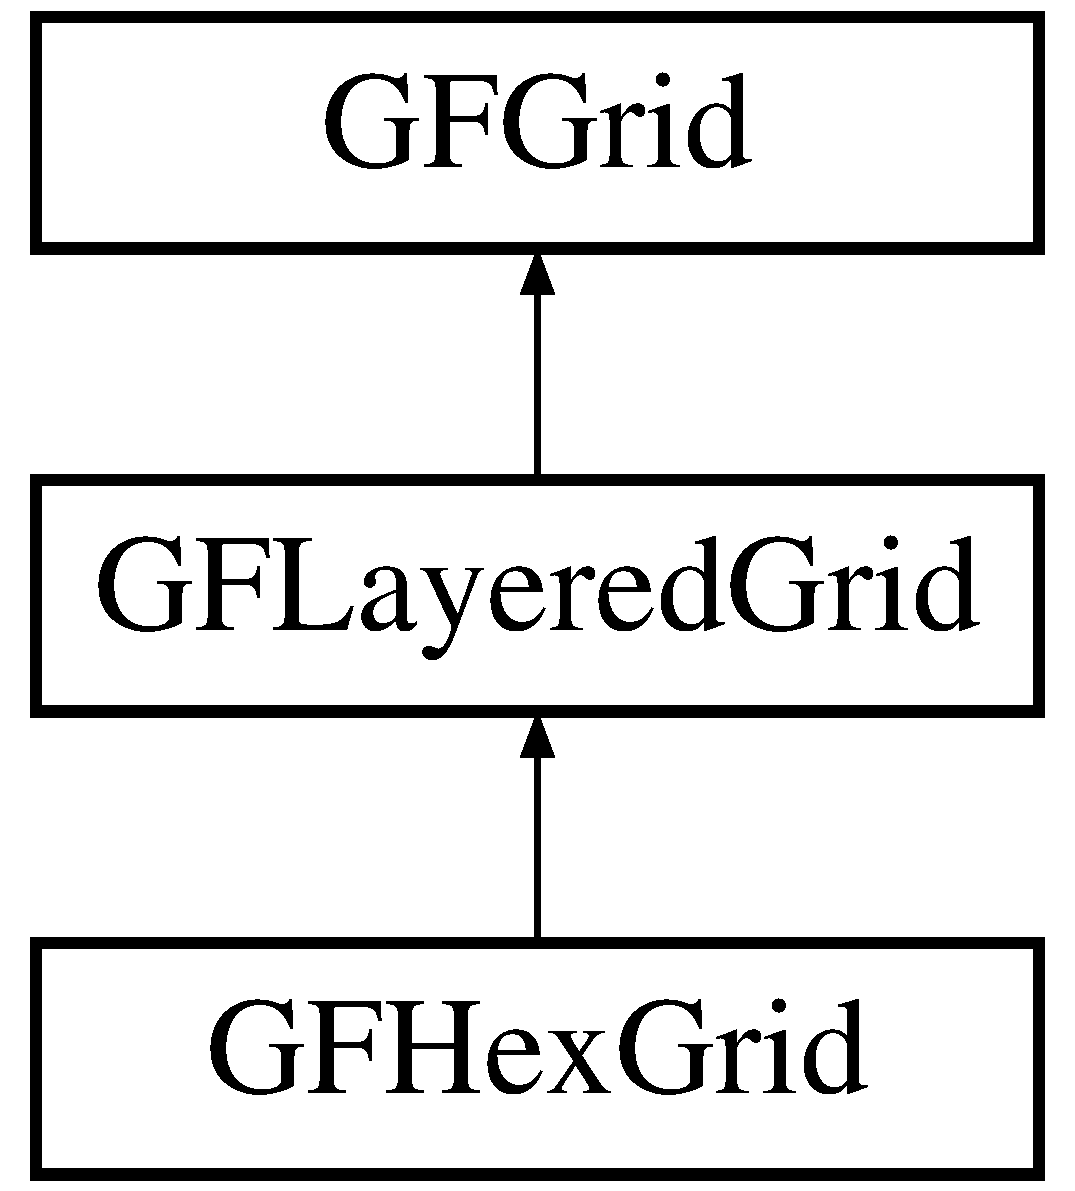
\includegraphics[height=3.000000cm]{class_g_f_hex_grid}
\end{center}
\end{figure}
\subsection*{Public Types}
\begin{DoxyCompactItemize}
\item 
enum \hyperlink{class_g_f_hex_grid_af3503ff5abb4dc3569875daa37dfd6e6_af3503ff5abb4dc3569875daa37dfd6e6}{Hex\+Orientation} \{ \hyperlink{class_g_f_hex_grid_af3503ff5abb4dc3569875daa37dfd6e6_af3503ff5abb4dc3569875daa37dfd6e6ae072b74647674927337f70f1f6af0666}{Hex\+Orientation.\+Pointy\+Sides}, 
\hyperlink{class_g_f_hex_grid_af3503ff5abb4dc3569875daa37dfd6e6_af3503ff5abb4dc3569875daa37dfd6e6a94a6b60f9e84da01af0db39053695834}{Hex\+Orientation.\+Flat\+Sides}
 \}
\begin{DoxyCompactList}\small\item\em orientation of hexes, pointy or flat sides.\end{DoxyCompactList}\item 
enum \hyperlink{class_g_f_hex_grid_aa82586fdc2de52a215609e48abcc265a_aa82586fdc2de52a215609e48abcc265a}{Hex\+Top\+Orientation} \{ \hyperlink{class_g_f_hex_grid_aa82586fdc2de52a215609e48abcc265a_aa82586fdc2de52a215609e48abcc265aa6474d6b6b7acbea9c60c3d0b941758ee}{Hex\+Top\+Orientation.\+Flat\+Tops}, 
\hyperlink{class_g_f_hex_grid_aa82586fdc2de52a215609e48abcc265a_aa82586fdc2de52a215609e48abcc265aaa2350be1698837b593a283f2eaf13c36}{Hex\+Top\+Orientation.\+Pointy\+Tops}
 \}
\begin{DoxyCompactList}\small\item\em orientation of hexes, flat or pointy tops.\end{DoxyCompactList}\item 
enum \hyperlink{class_g_f_hex_grid_a6394c0f75370f3b02e437f28e52127d7_a6394c0f75370f3b02e437f28e52127d7}{Hex\+Grid\+Shape} \{ \\*
\hyperlink{class_g_f_hex_grid_a6394c0f75370f3b02e437f28e52127d7_a6394c0f75370f3b02e437f28e52127d7ace9291906a4c3b042650b70d7f3b152e}{Hex\+Grid\+Shape.\+Rectangle}, 
\hyperlink{class_g_f_hex_grid_a6394c0f75370f3b02e437f28e52127d7_a6394c0f75370f3b02e437f28e52127d7aced30051e070abc63cbc6d897b26c5e2}{Hex\+Grid\+Shape.\+Compact\+Rectangle}, 
\hyperlink{class_g_f_hex_grid_a6394c0f75370f3b02e437f28e52127d7_a6394c0f75370f3b02e437f28e52127d7a37fe777298b67f1b38eb7a718952df65}{Hex\+Grid\+Shape.\+Rectangle\+Down}, 
\hyperlink{class_g_f_hex_grid_a6394c0f75370f3b02e437f28e52127d7_a6394c0f75370f3b02e437f28e52127d7ad62e74b4f4bdc571fb184229772ea930}{Hex\+Grid\+Shape.\+Rhombus}, 
\\*
\hyperlink{class_g_f_hex_grid_a6394c0f75370f3b02e437f28e52127d7_a6394c0f75370f3b02e437f28e52127d7af2ae57405fde1821d059aaf78fedcb84}{Hex\+Grid\+Shape.\+Rhombus\+Down}, 
\hyperlink{class_g_f_hex_grid_a6394c0f75370f3b02e437f28e52127d7_a6394c0f75370f3b02e437f28e52127d7a766ba0e1e70b9f2fc1204ef785859e19}{Hex\+Grid\+Shape.\+Herringbone\+Up}, 
\hyperlink{class_g_f_hex_grid_a6394c0f75370f3b02e437f28e52127d7_a6394c0f75370f3b02e437f28e52127d7a9a6695df59ef6afb4c18995c44b97875}{Hex\+Grid\+Shape.\+Herringbone\+Down}
 \}
\item 
enum \hyperlink{class_g_f_hex_grid_a4591076c54ef7c3b01f61f47ceb6439f_a4591076c54ef7c3b01f61f47ceb6439f}{Hex\+Direction} \{ \\*
\hyperlink{class_g_f_hex_grid_a4591076c54ef7c3b01f61f47ceb6439f_a4591076c54ef7c3b01f61f47ceb6439fa8d9c307cb7f3c4a32822a51922d1ceaa}{Hex\+Direction.\+N}, 
\hyperlink{class_g_f_hex_grid_a4591076c54ef7c3b01f61f47ceb6439f_a4591076c54ef7c3b01f61f47ceb6439fadc33066c3993e0d50896e533fd692ce0}{Hex\+Direction.\+N\+E}, 
\hyperlink{class_g_f_hex_grid_a4591076c54ef7c3b01f61f47ceb6439f_a4591076c54ef7c3b01f61f47ceb6439fa3a3ea00cfc35332cedf6e5e9a32e94da}{Hex\+Direction.\+E}, 
\hyperlink{class_g_f_hex_grid_a4591076c54ef7c3b01f61f47ceb6439f_a4591076c54ef7c3b01f61f47ceb6439faf003c44deab679aa2edfaff864c77402}{Hex\+Direction.\+S\+E}, 
\\*
\hyperlink{class_g_f_hex_grid_a4591076c54ef7c3b01f61f47ceb6439f_a4591076c54ef7c3b01f61f47ceb6439fa5dbc98dcc983a70728bd082d1a47546e}{Hex\+Direction.\+S}, 
\hyperlink{class_g_f_hex_grid_a4591076c54ef7c3b01f61f47ceb6439f_a4591076c54ef7c3b01f61f47ceb6439fa6f56aa4e2561eb66f17f6d8de8070a77}{Hex\+Direction.\+S\+W}, 
\hyperlink{class_g_f_hex_grid_a4591076c54ef7c3b01f61f47ceb6439f_a4591076c54ef7c3b01f61f47ceb6439fa61e9c06ea9a85a5088a499df6458d276}{Hex\+Direction.\+W}, 
\hyperlink{class_g_f_hex_grid_a4591076c54ef7c3b01f61f47ceb6439f_a4591076c54ef7c3b01f61f47ceb6439fa7f39ac71e81132daad44925b3bdfde5a}{Hex\+Direction.\+N\+W}
 \}
\begin{DoxyCompactList}\small\item\em Cardinal direction of a vertex.\end{DoxyCompactList}\end{DoxyCompactItemize}
\subsection*{Public Member Functions}
\begin{DoxyCompactItemize}
\item 
override Vector3 \hyperlink{class_g_f_hex_grid_a476548c7582c1529de47f31ce891f4fd_a476548c7582c1529de47f31ce891f4fd}{World\+To\+Grid} (Vector3 world\+Point)
\begin{DoxyCompactList}\small\item\em Converts world coordinates to grid coordinates.\end{DoxyCompactList}\item 
override Vector3 \hyperlink{class_g_f_hex_grid_abac4ca6dba9e7ee8ed87f70cf4a7afc7_abac4ca6dba9e7ee8ed87f70cf4a7afc7}{Grid\+To\+World} (Vector3 grid\+Point)
\begin{DoxyCompactList}\small\item\em Converts grid coordinates to world coordinates\end{DoxyCompactList}\item 
Vector3 \hyperlink{class_g_f_hex_grid_aa824605cf4179ec0c45eb030496ec3fb_aa824605cf4179ec0c45eb030496ec3fb}{World\+To\+Herring\+U} (Vector3 world)
\begin{DoxyCompactList}\small\item\em Returns the upwards herringbone coordinates of a point in world space.\end{DoxyCompactList}\item 
Vector3 \hyperlink{class_g_f_hex_grid_a40d8289d887c12c1fd95b3ec818ed22a_a40d8289d887c12c1fd95b3ec818ed22a}{World\+To\+Herring\+D} (Vector3 world)
\begin{DoxyCompactList}\small\item\em Returns the downwards herringbone coordinates of a point in world space.\end{DoxyCompactList}\item 
Vector3 \hyperlink{class_g_f_hex_grid_a1669b77f20e1406b7d7554d45635945e_a1669b77f20e1406b7d7554d45635945e}{World\+To\+Rhombic} (Vector3 world)
\begin{DoxyCompactList}\small\item\em Returns the rhombic coordinates of a point in world space.\end{DoxyCompactList}\item 
Vector3 \hyperlink{class_g_f_hex_grid_a72549876d8ef493279002dc04ecc2332_a72549876d8ef493279002dc04ecc2332}{World\+To\+Rhombic\+D} (Vector3 world)
\begin{DoxyCompactList}\small\item\em Returns the downwards rhombic coordinates of a point in world space.\end{DoxyCompactList}\item 
Vector4 \hyperlink{class_g_f_hex_grid_a77f39b12ba07df6135bd28941e30d9ff_a77f39b12ba07df6135bd28941e30d9ff}{World\+To\+Cubic} (Vector3 world)
\begin{DoxyCompactList}\small\item\em Returns the cubic coordinates of a point in world space.\end{DoxyCompactList}\item 
Vector3 \hyperlink{class_g_f_hex_grid_a376663e9575f6e1f3937c7f768070a5c_a376663e9575f6e1f3937c7f768070a5c}{Herring\+U\+To\+World} (Vector3 herring)
\begin{DoxyCompactList}\small\item\em Returns the world coordinates of a point in upwards herringbone coordinates.\end{DoxyCompactList}\item 
Vector3 \hyperlink{class_g_f_hex_grid_a261551484b05ea71dcc5b442dbf2e0f0_a261551484b05ea71dcc5b442dbf2e0f0}{Herring\+U\+To\+Herring\+D} (Vector3 herring)
\begin{DoxyCompactList}\small\item\em Returns the downwards herringbone coordinates of a point in upwards-\/ coordinates.\end{DoxyCompactList}\item 
Vector3 \hyperlink{class_g_f_hex_grid_a5352c5998878b421c1d117958ca2591d_a5352c5998878b421c1d117958ca2591d}{Herring\+U\+To\+Rhombic} (Vector3 herring)
\begin{DoxyCompactList}\small\item\em Returns the rhombic coordinates of a point in upwards herringbone coordinates.\end{DoxyCompactList}\item 
Vector3 \hyperlink{class_g_f_hex_grid_aff4d8a69e8a6dca3c4364338e5fef855_aff4d8a69e8a6dca3c4364338e5fef855}{Herring\+U\+To\+Rhombic\+D} (Vector3 herring)
\begin{DoxyCompactList}\small\item\em Returns the downwards rhombic coordinates of a point in upwards herringbone coordinates.\end{DoxyCompactList}\item 
Vector4 \hyperlink{class_g_f_hex_grid_af755aa27158a1b137c1f45b65a780d03_af755aa27158a1b137c1f45b65a780d03}{Herring\+U\+To\+Cubic} (Vector3 herring)
\begin{DoxyCompactList}\small\item\em Returns the cubic coordinates of a point in upwards herringbone coordinates.\end{DoxyCompactList}\item 
Vector3 \hyperlink{class_g_f_hex_grid_a23e68e317c4004a146e2cbafb6bc56c0_a23e68e317c4004a146e2cbafb6bc56c0}{Herring\+D\+To\+World} (Vector3 herring)
\begin{DoxyCompactList}\small\item\em Returns the world coordinates of a point in downwards herringbone coordinates.\end{DoxyCompactList}\item 
Vector3 \hyperlink{class_g_f_hex_grid_ab68b4ecc340f6014bba1ac6851921c34_ab68b4ecc340f6014bba1ac6851921c34}{Herring\+D\+To\+Herring\+U} (Vector3 herring)
\begin{DoxyCompactList}\small\item\em Returns the upwards herringbone coordinates of a point in downwards-\/ coordinates.\end{DoxyCompactList}\item 
Vector3 \hyperlink{class_g_f_hex_grid_a9113159acea48cf847a3e8e50828bbf7_a9113159acea48cf847a3e8e50828bbf7}{Herring\+D\+To\+Rhombic} (Vector3 herring)
\begin{DoxyCompactList}\small\item\em Returns the rhombic coordinates of a point in downwards herringbone coordinates.\end{DoxyCompactList}\item 
Vector3 \hyperlink{class_g_f_hex_grid_a8ee594b22885339e63dfcefc9efe90b5_a8ee594b22885339e63dfcefc9efe90b5}{Herring\+D\+To\+Rhombic\+D} (Vector3 herring)
\begin{DoxyCompactList}\small\item\em Returns the downwards rhombic coordinates of a point in downwards herringbone coordinates.\end{DoxyCompactList}\item 
Vector4 \hyperlink{class_g_f_hex_grid_a0105d03d663f6e3086d0a6a0cde650f5_a0105d03d663f6e3086d0a6a0cde650f5}{Herring\+D\+To\+Cubic} (Vector3 herring)
\begin{DoxyCompactList}\small\item\em Returns the cubic coordinates of a point in downwards herringbone coordinates.\end{DoxyCompactList}\item 
Vector3 \hyperlink{class_g_f_hex_grid_af8215888f6f22eccc2da17f0984fb5c1_af8215888f6f22eccc2da17f0984fb5c1}{Rhombic\+To\+World} (Vector3 rhombic)
\begin{DoxyCompactList}\small\item\em Returns the world coordinates of a point in rhombic coordinates.\end{DoxyCompactList}\item 
Vector3 \hyperlink{class_g_f_hex_grid_a95e3f6b72b073af645cd7ebe301a133c_a95e3f6b72b073af645cd7ebe301a133c}{Rhombic\+To\+Herring\+U} (Vector3 rhombic)
\begin{DoxyCompactList}\small\item\em Returns the upwards herringbone coordinates of a point in rhombic coordinates.\end{DoxyCompactList}\item 
Vector3 \hyperlink{class_g_f_hex_grid_ad7bf26ea21e55594a011899d72a1a305_ad7bf26ea21e55594a011899d72a1a305}{Rhombic\+To\+Rhombic\+D} (Vector3 rhombic)
\begin{DoxyCompactList}\small\item\em Returns the downwards rhombic coordinates of a point in rhombic coordinates.\end{DoxyCompactList}\item 
Vector3 \hyperlink{class_g_f_hex_grid_a3d2722a9ce23d0769ae92812ecdecb34_a3d2722a9ce23d0769ae92812ecdecb34}{Rhombic\+To\+Herring\+D} (Vector3 rhombic)
\begin{DoxyCompactList}\small\item\em Returns the downwards herringbone coordinates of a point in rhombic coordinates.\end{DoxyCompactList}\item 
Vector4 \hyperlink{class_g_f_hex_grid_a1ff9f3d11d707bc0d434d07a2df92549_a1ff9f3d11d707bc0d434d07a2df92549}{Rhombic\+To\+Cubic} (Vector3 rhombic)
\begin{DoxyCompactList}\small\item\em Returns the cubic coordinates of a point in rhombic coordinates.\end{DoxyCompactList}\item 
Vector3 \hyperlink{class_g_f_hex_grid_aae1b996c067ade686279c48f6588cf08_aae1b996c067ade686279c48f6588cf08}{Rhombic\+D\+To\+World} (Vector3 rhombic)
\begin{DoxyCompactList}\small\item\em Returns the world coordinates of a point in downwards rhombic coordinates.\end{DoxyCompactList}\item 
Vector3 \hyperlink{class_g_f_hex_grid_a0f748078789813bf09541328e0aaae53_a0f748078789813bf09541328e0aaae53}{Rhombic\+D\+To\+Herring\+U} (Vector3 rhombic)
\begin{DoxyCompactList}\small\item\em Returns the upwards herringbone coordinates of a point in downwards rhombic coordinates.\end{DoxyCompactList}\item 
Vector3 \hyperlink{class_g_f_hex_grid_a17af97050751d292ba61ac0629243da0_a17af97050751d292ba61ac0629243da0}{Rhombic\+D\+To\+Herring\+D} (Vector3 rhombic)
\begin{DoxyCompactList}\small\item\em Returns the downwards herringbone coordinates of a point in downwards rhombic coordinates.\end{DoxyCompactList}\item 
Vector3 \hyperlink{class_g_f_hex_grid_a92465d198faca2652e51c726acb94efe_a92465d198faca2652e51c726acb94efe}{Rhombic\+D\+To\+Rhombic} (Vector3 rhombic)
\begin{DoxyCompactList}\small\item\em Returns the downwards herringbone coordinates of a point in downwards rhombic coordinates.\end{DoxyCompactList}\item 
Vector4 \hyperlink{class_g_f_hex_grid_a5e48d303cdd36b6621c572152123183b_a5e48d303cdd36b6621c572152123183b}{Rhombic\+D\+To\+Cubic} (Vector3 rhombic)
\begin{DoxyCompactList}\small\item\em Returns the cubic coordinates of a point in downwards rhombic coordinates.\end{DoxyCompactList}\item 
Vector3 \hyperlink{class_g_f_hex_grid_a7a59e6279ccbb14fbae1a053395b14ae_a7a59e6279ccbb14fbae1a053395b14ae}{Cubic\+To\+World} (Vector4 cubic)
\begin{DoxyCompactList}\small\item\em Returns the world coordinates of a point in cubic coordinates.\end{DoxyCompactList}\item 
Vector3 \hyperlink{class_g_f_hex_grid_a72c80c9cc6baa0183cc023d069049370_a72c80c9cc6baa0183cc023d069049370}{Cubic\+To\+Herring\+U} (Vector4 cubic)
\begin{DoxyCompactList}\small\item\em Returns the upwards herring coordinates of a point in cubic coordinates.\end{DoxyCompactList}\item 
Vector3 \hyperlink{class_g_f_hex_grid_a397fa739ccb7cd8fd68c82203bc2838a_a397fa739ccb7cd8fd68c82203bc2838a}{Cubic\+To\+Rhombic} (Vector4 cubic)
\begin{DoxyCompactList}\small\item\em Returns the rhombic coordinates of a point in cubic coordinates.\end{DoxyCompactList}\item 
Vector3 \hyperlink{class_g_f_hex_grid_a9f918153c4d8b1092bb5b32c91e88ee5_a9f918153c4d8b1092bb5b32c91e88ee5}{Cubic\+To\+Rhombic\+D} (Vector4 cubic)
\begin{DoxyCompactList}\small\item\em Returns the downwards rhombic coordinates of a point in cubic coordinates.\end{DoxyCompactList}\item 
override Vector3 \hyperlink{class_g_f_hex_grid_aa3e803a3567facf12848c80698ae72ae_aa3e803a3567facf12848c80698ae72ae}{Nearest\+Vertex\+W} (Vector3 world, bool do\+Debug=false)
\begin{DoxyCompactList}\small\item\em Returns the world coordinates of the nearest vertex.\end{DoxyCompactList}\item 
override Vector3 \hyperlink{class_g_f_hex_grid_ad8c205a56bc277236e0c3d1c6cb44845_ad8c205a56bc277236e0c3d1c6cb44845}{Nearest\+Face\+W} (Vector3 world, bool do\+Debug)
\begin{DoxyCompactList}\small\item\em Returns the world coordinates of the nearest face.\end{DoxyCompactList}\item 
override Vector3 \hyperlink{class_g_f_hex_grid_a58ce4a0c91753d5457c4df0ebaac90a9_a58ce4a0c91753d5457c4df0ebaac90a9}{Nearest\+Box\+W} (Vector3 from\+Point, bool do\+Debug)
\begin{DoxyCompactList}\small\item\em Returns the world coordinates of the nearest box.\end{DoxyCompactList}\item 
override Vector3 \hyperlink{class_g_f_hex_grid_ae335a549959829d91dcede4847d7168f_ae335a549959829d91dcede4847d7168f}{Nearest\+Vertex\+G} (Vector3 world)
\begin{DoxyCompactList}\small\item\em Returns the grid position of the nearest vertex.\end{DoxyCompactList}\item 
override Vector3 \hyperlink{class_g_f_hex_grid_abd6193db6b434b5a2ce3512c45faa0b1_abd6193db6b434b5a2ce3512c45faa0b1}{Nearest\+Face\+G} (Vector3 world)
\begin{DoxyCompactList}\small\item\em Returns the grid position of the nearest face.\end{DoxyCompactList}\item 
override Vector3 \hyperlink{class_g_f_hex_grid_ab038b99bc1bedfcdee8a0736c4ed1a1e_ab038b99bc1bedfcdee8a0736c4ed1a1e}{Nearest\+Box\+G} (Vector3 world)
\begin{DoxyCompactList}\small\item\em Returns the grid position of the nearest box.\end{DoxyCompactList}\item 
Vector3 \hyperlink{class_g_f_hex_grid_a62d5c4c11737bc2bb81275e7b601773c_a62d5c4c11737bc2bb81275e7b601773c}{Nearest\+Vertex\+H\+O} (Vector3 world)
\begin{DoxyCompactList}\small\item\em Returns the upwards herring position of the nearest vertex.\end{DoxyCompactList}\item 
Vector3 \hyperlink{class_g_f_hex_grid_a23a792a9788102c3af99a5de5b61a982_a23a792a9788102c3af99a5de5b61a982}{Nearest\+Face\+H\+O} (Vector3 world)
\begin{DoxyCompactList}\small\item\em Returns the upwards herring position of the nearest face.\end{DoxyCompactList}\item 
Vector3 \hyperlink{class_g_f_hex_grid_a37ab0165e6b0dba047a7493e5862912d_a37ab0165e6b0dba047a7493e5862912d}{Nearest\+Box\+H\+O} (Vector3 world)
\begin{DoxyCompactList}\small\item\em Returns the grid position of the nearest box.\end{DoxyCompactList}\item 
Vector3 \hyperlink{class_g_f_hex_grid_a1a6a188b62d970eb084eb0907ad5d16e_a1a6a188b62d970eb084eb0907ad5d16e}{Nearest\+Vertex\+R} (Vector3 world)
\begin{DoxyCompactList}\small\item\em Returns the rhombic position of the nearest vertex.\end{DoxyCompactList}\item 
Vector3 \hyperlink{class_g_f_hex_grid_a2cf1f2642ac2dea0058fee159ea7e78b_a2cf1f2642ac2dea0058fee159ea7e78b}{Nearest\+Face\+R} (Vector3 world)
\begin{DoxyCompactList}\small\item\em Returns the rhombic position of the nearest face.\end{DoxyCompactList}\item 
Vector3 \hyperlink{class_g_f_hex_grid_aa6a007fdbe6772fe4df1c906b2cdb47f_aa6a007fdbe6772fe4df1c906b2cdb47f}{Nearest\+Box\+R} (Vector3 world)
\begin{DoxyCompactList}\small\item\em Returns the rhombic position of the nearest box.\end{DoxyCompactList}\item 
Vector4 \hyperlink{class_g_f_hex_grid_aa5d236ca39c81d71f7f088dda68c9aa5_aa5d236ca39c81d71f7f088dda68c9aa5}{Nearest\+Vertex\+C} (Vector3 world)
\begin{DoxyCompactList}\small\item\em Returns the cubic position of the nearest vertex.\end{DoxyCompactList}\item 
Vector4 \hyperlink{class_g_f_hex_grid_ac70e0c7e710fbc3ed4748911eded9bf0_ac70e0c7e710fbc3ed4748911eded9bf0}{Nearest\+Face\+C} (Vector3 world)
\begin{DoxyCompactList}\small\item\em Returns the cubic position of the nearest face.\end{DoxyCompactList}\item 
Vector4 \hyperlink{class_g_f_hex_grid_a8901857400ef5fb8673a2b6ca5aaa52d_a8901857400ef5fb8673a2b6ca5aaa52d}{Nearest\+Box\+C} (Vector3 world)
\begin{DoxyCompactList}\small\item\em Returns the cubic position of the nearest box.\end{DoxyCompactList}\item 
override Vector3 \hyperlink{class_g_f_hex_grid_a2d51f41dc859b4957bb67a518c252632_a2d51f41dc859b4957bb67a518c252632}{Align\+Vector3} (Vector3 pos, Vector3 scale, \hyperlink{class_grid_framework_1_1_vectors_1_1_bool_vector3}{Bool\+Vector3} lock\+Axis)
\begin{DoxyCompactList}\small\item\em Fits a position vector into the grid.\end{DoxyCompactList}\item 
override Vector3 \hyperlink{class_g_f_hex_grid_a534e73e65f65a117ebb6f4e1122f097d_a534e73e65f65a117ebb6f4e1122f097d}{Scale\+Vector3} (Vector3 scl, \hyperlink{class_grid_framework_1_1_vectors_1_1_bool_vector3}{Bool\+Vector3} lock\+Axis)
\begin{DoxyCompactList}\small\item\em Scales a size vector to fit inside a grid.\end{DoxyCompactList}\end{DoxyCompactItemize}
\subsection*{Properties}
\begin{DoxyCompactItemize}
\item 
float \hyperlink{class_g_f_hex_grid_a99701e2998e2b7305bb1bbe0c1ef9506_a99701e2998e2b7305bb1bbe0c1ef9506}{radius}\hspace{0.3cm}{\ttfamily  \mbox{[}get, set\mbox{]}}
\begin{DoxyCompactList}\small\item\em Distance from the centre of a hex to a vertex.\end{DoxyCompactList}\item 
\hyperlink{class_g_f_hex_grid_af3503ff5abb4dc3569875daa37dfd6e6_af3503ff5abb4dc3569875daa37dfd6e6}{Hex\+Orientation} \hyperlink{class_g_f_hex_grid_a1c7aee0c19fe71879a1056d1c04be420_a1c7aee0c19fe71879a1056d1c04be420}{hex\+Side\+Mode}\hspace{0.3cm}{\ttfamily  \mbox{[}get, set\mbox{]}}
\begin{DoxyCompactList}\small\item\em Pointy sides or flat sides.\end{DoxyCompactList}\item 
\hyperlink{class_g_f_hex_grid_aa82586fdc2de52a215609e48abcc265a_aa82586fdc2de52a215609e48abcc265a}{Hex\+Top\+Orientation} \hyperlink{class_g_f_hex_grid_a651e7fbf9e12e4d8fd31f21503aeb120_a651e7fbf9e12e4d8fd31f21503aeb120}{hex\+Top\+Mode}\hspace{0.3cm}{\ttfamily  \mbox{[}get, set\mbox{]}}
\begin{DoxyCompactList}\small\item\em Flat tops or pointy tops.\end{DoxyCompactList}\item 
\hyperlink{class_g_f_hex_grid_a6394c0f75370f3b02e437f28e52127d7_a6394c0f75370f3b02e437f28e52127d7}{Hex\+Grid\+Shape} \hyperlink{class_g_f_hex_grid_aa655390c4d3e1872978c50b964107dff_aa655390c4d3e1872978c50b964107dff}{grid\+Style}\hspace{0.3cm}{\ttfamily  \mbox{[}get, set\mbox{]}}
\begin{DoxyCompactList}\small\item\em The shape of the overall grid, affects only drawing and rendering, not the calculations.\end{DoxyCompactList}\item 
float \hyperlink{class_g_f_hex_grid_a09ba217a58d06021fe82fed119c96969_a09ba217a58d06021fe82fed119c96969}{side}\hspace{0.3cm}{\ttfamily  \mbox{[}get\mbox{]}}
\begin{DoxyCompactList}\small\item\em 1.\+5 times the radius.\end{DoxyCompactList}\item 
float \hyperlink{class_g_f_hex_grid_adef19e30b8a5c7e243d1f8239e270630_adef19e30b8a5c7e243d1f8239e270630}{height}\hspace{0.3cm}{\ttfamily  \mbox{[}get\mbox{]}}
\begin{DoxyCompactList}\small\item\em Full width of the hex.\end{DoxyCompactList}\item 
float \hyperlink{class_g_f_hex_grid_a6d9ef76fc36e9b3709feb605219672a7_a6d9ef76fc36e9b3709feb605219672a7}{width}\hspace{0.3cm}{\ttfamily  \mbox{[}get\mbox{]}}
\begin{DoxyCompactList}\small\item\em Distance between vertices on opposite sides.\end{DoxyCompactList}\end{DoxyCompactItemize}
\subsection*{Additional Inherited Members}


\subsection{Detailed Description}
A regular hexagonal grid that forms a honeycomb pattern. It is characterized by the {\ttfamily radius} (distance from the centre of a hexagon to one of its vertices) and the {\ttfamily depth} (distance between two honeycomb layers). Hex grids use a herringbone pattern for their coordinate system, please refer to the user manual for information about how that coordinate system works. 

\subsection{Member Enumeration Documentation}
\hypertarget{class_g_f_hex_grid_a4591076c54ef7c3b01f61f47ceb6439f_a4591076c54ef7c3b01f61f47ceb6439f}{\index{G\+F\+Hex\+Grid@{G\+F\+Hex\+Grid}!Hex\+Direction@{Hex\+Direction}}
\index{Hex\+Direction@{Hex\+Direction}!G\+F\+Hex\+Grid@{G\+F\+Hex\+Grid}}
\subsubsection[{Hex\+Direction}]{\setlength{\rightskip}{0pt plus 5cm}enum {\bf G\+F\+Hex\+Grid.\+Hex\+Direction}}}\label{class_g_f_hex_grid_a4591076c54ef7c3b01f61f47ceb6439f_a4591076c54ef7c3b01f61f47ceb6439f}
The cardinal position of a vertex relative to the centre of a given hex. Note that using N and S for pointy sides, as well as E and W for flat sides does not make sense, but it is still possible. \begin{Desc}
\item[Enumerator]\par
\begin{description}
\index{N@{N}!G\+F\+Hex\+Grid@{G\+F\+Hex\+Grid}}\index{G\+F\+Hex\+Grid@{G\+F\+Hex\+Grid}!N@{N}}\item[{\em 
\hypertarget{class_g_f_hex_grid_a4591076c54ef7c3b01f61f47ceb6439f_a4591076c54ef7c3b01f61f47ceb6439fa8d9c307cb7f3c4a32822a51922d1ceaa}{N}\label{class_g_f_hex_grid_a4591076c54ef7c3b01f61f47ceb6439f_a4591076c54ef7c3b01f61f47ceb6439fa8d9c307cb7f3c4a32822a51922d1ceaa}
}]North. \index{N\+E@{N\+E}!G\+F\+Hex\+Grid@{G\+F\+Hex\+Grid}}\index{G\+F\+Hex\+Grid@{G\+F\+Hex\+Grid}!N\+E@{N\+E}}\item[{\em 
\hypertarget{class_g_f_hex_grid_a4591076c54ef7c3b01f61f47ceb6439f_a4591076c54ef7c3b01f61f47ceb6439fadc33066c3993e0d50896e533fd692ce0}{N\+E}\label{class_g_f_hex_grid_a4591076c54ef7c3b01f61f47ceb6439f_a4591076c54ef7c3b01f61f47ceb6439fadc33066c3993e0d50896e533fd692ce0}
}]South. \index{E@{E}!G\+F\+Hex\+Grid@{G\+F\+Hex\+Grid}}\index{G\+F\+Hex\+Grid@{G\+F\+Hex\+Grid}!E@{E}}\item[{\em 
\hypertarget{class_g_f_hex_grid_a4591076c54ef7c3b01f61f47ceb6439f_a4591076c54ef7c3b01f61f47ceb6439fa3a3ea00cfc35332cedf6e5e9a32e94da}{E}\label{class_g_f_hex_grid_a4591076c54ef7c3b01f61f47ceb6439f_a4591076c54ef7c3b01f61f47ceb6439fa3a3ea00cfc35332cedf6e5e9a32e94da}
}]East. \index{S\+E@{S\+E}!G\+F\+Hex\+Grid@{G\+F\+Hex\+Grid}}\index{G\+F\+Hex\+Grid@{G\+F\+Hex\+Grid}!S\+E@{S\+E}}\item[{\em 
\hypertarget{class_g_f_hex_grid_a4591076c54ef7c3b01f61f47ceb6439f_a4591076c54ef7c3b01f61f47ceb6439faf003c44deab679aa2edfaff864c77402}{S\+E}\label{class_g_f_hex_grid_a4591076c54ef7c3b01f61f47ceb6439f_a4591076c54ef7c3b01f61f47ceb6439faf003c44deab679aa2edfaff864c77402}
}]South-\/\+East. \index{S@{S}!G\+F\+Hex\+Grid@{G\+F\+Hex\+Grid}}\index{G\+F\+Hex\+Grid@{G\+F\+Hex\+Grid}!S@{S}}\item[{\em 
\hypertarget{class_g_f_hex_grid_a4591076c54ef7c3b01f61f47ceb6439f_a4591076c54ef7c3b01f61f47ceb6439fa5dbc98dcc983a70728bd082d1a47546e}{S}\label{class_g_f_hex_grid_a4591076c54ef7c3b01f61f47ceb6439f_a4591076c54ef7c3b01f61f47ceb6439fa5dbc98dcc983a70728bd082d1a47546e}
}]South. \index{S\+W@{S\+W}!G\+F\+Hex\+Grid@{G\+F\+Hex\+Grid}}\index{G\+F\+Hex\+Grid@{G\+F\+Hex\+Grid}!S\+W@{S\+W}}\item[{\em 
\hypertarget{class_g_f_hex_grid_a4591076c54ef7c3b01f61f47ceb6439f_a4591076c54ef7c3b01f61f47ceb6439fa6f56aa4e2561eb66f17f6d8de8070a77}{S\+W}\label{class_g_f_hex_grid_a4591076c54ef7c3b01f61f47ceb6439f_a4591076c54ef7c3b01f61f47ceb6439fa6f56aa4e2561eb66f17f6d8de8070a77}
}]South-\/\+West. \index{W@{W}!G\+F\+Hex\+Grid@{G\+F\+Hex\+Grid}}\index{G\+F\+Hex\+Grid@{G\+F\+Hex\+Grid}!W@{W}}\item[{\em 
\hypertarget{class_g_f_hex_grid_a4591076c54ef7c3b01f61f47ceb6439f_a4591076c54ef7c3b01f61f47ceb6439fa61e9c06ea9a85a5088a499df6458d276}{W}\label{class_g_f_hex_grid_a4591076c54ef7c3b01f61f47ceb6439f_a4591076c54ef7c3b01f61f47ceb6439fa61e9c06ea9a85a5088a499df6458d276}
}]West. \index{N\+W@{N\+W}!G\+F\+Hex\+Grid@{G\+F\+Hex\+Grid}}\index{G\+F\+Hex\+Grid@{G\+F\+Hex\+Grid}!N\+W@{N\+W}}\item[{\em 
\hypertarget{class_g_f_hex_grid_a4591076c54ef7c3b01f61f47ceb6439f_a4591076c54ef7c3b01f61f47ceb6439fa7f39ac71e81132daad44925b3bdfde5a}{N\+W}\label{class_g_f_hex_grid_a4591076c54ef7c3b01f61f47ceb6439f_a4591076c54ef7c3b01f61f47ceb6439fa7f39ac71e81132daad44925b3bdfde5a}
}]North-\/\+West. \end{description}
\end{Desc}
\hypertarget{class_g_f_hex_grid_a6394c0f75370f3b02e437f28e52127d7_a6394c0f75370f3b02e437f28e52127d7}{\index{G\+F\+Hex\+Grid@{G\+F\+Hex\+Grid}!Hex\+Grid\+Shape@{Hex\+Grid\+Shape}}
\index{Hex\+Grid\+Shape@{Hex\+Grid\+Shape}!G\+F\+Hex\+Grid@{G\+F\+Hex\+Grid}}
\subsubsection[{Hex\+Grid\+Shape}]{\setlength{\rightskip}{0pt plus 5cm}enum {\bf G\+F\+Hex\+Grid.\+Hex\+Grid\+Shape}}}\label{class_g_f_hex_grid_a6394c0f75370f3b02e437f28e52127d7_a6394c0f75370f3b02e437f28e52127d7}
summary$>$Shape of the drawing and rendering.

Different shapes of hexagonal grids\+: {\ttfamily Rectangle} looks like a rectangle with every odd-\/numbered column offset, {\ttfamily Compact\+Rectangle} is similar with the odd-\/numbered colums one hex shorter. \begin{Desc}
\item[Enumerator]\par
\begin{description}
\index{Rectangle@{Rectangle}!G\+F\+Hex\+Grid@{G\+F\+Hex\+Grid}}\index{G\+F\+Hex\+Grid@{G\+F\+Hex\+Grid}!Rectangle@{Rectangle}}\item[{\em 
\hypertarget{class_g_f_hex_grid_a6394c0f75370f3b02e437f28e52127d7_a6394c0f75370f3b02e437f28e52127d7ace9291906a4c3b042650b70d7f3b152e}{Rectangle}\label{class_g_f_hex_grid_a6394c0f75370f3b02e437f28e52127d7_a6394c0f75370f3b02e437f28e52127d7ace9291906a4c3b042650b70d7f3b152e}
}]Rectangular upwards herringbone pattern. \index{Compact\+Rectangle@{Compact\+Rectangle}!G\+F\+Hex\+Grid@{G\+F\+Hex\+Grid}}\index{G\+F\+Hex\+Grid@{G\+F\+Hex\+Grid}!Compact\+Rectangle@{Compact\+Rectangle}}\item[{\em 
\hypertarget{class_g_f_hex_grid_a6394c0f75370f3b02e437f28e52127d7_a6394c0f75370f3b02e437f28e52127d7aced30051e070abc63cbc6d897b26c5e2}{Compact\+Rectangle}\label{class_g_f_hex_grid_a6394c0f75370f3b02e437f28e52127d7_a6394c0f75370f3b02e437f28e52127d7aced30051e070abc63cbc6d897b26c5e2}
}]Rectangular upwards herringbone pattern with the top of every odd column clipped. \index{Rectangle\+Down@{Rectangle\+Down}!G\+F\+Hex\+Grid@{G\+F\+Hex\+Grid}}\index{G\+F\+Hex\+Grid@{G\+F\+Hex\+Grid}!Rectangle\+Down@{Rectangle\+Down}}\item[{\em 
\hypertarget{class_g_f_hex_grid_a6394c0f75370f3b02e437f28e52127d7_a6394c0f75370f3b02e437f28e52127d7a37fe777298b67f1b38eb7a718952df65}{Rectangle\+Down}\label{class_g_f_hex_grid_a6394c0f75370f3b02e437f28e52127d7_a6394c0f75370f3b02e437f28e52127d7a37fe777298b67f1b38eb7a718952df65}
}]Rectangular downwards herringbone pattern. \index{Rhombus@{Rhombus}!G\+F\+Hex\+Grid@{G\+F\+Hex\+Grid}}\index{G\+F\+Hex\+Grid@{G\+F\+Hex\+Grid}!Rhombus@{Rhombus}}\item[{\em 
\hypertarget{class_g_f_hex_grid_a6394c0f75370f3b02e437f28e52127d7_a6394c0f75370f3b02e437f28e52127d7ad62e74b4f4bdc571fb184229772ea930}{Rhombus}\label{class_g_f_hex_grid_a6394c0f75370f3b02e437f28e52127d7_a6394c0f75370f3b02e437f28e52127d7ad62e74b4f4bdc571fb184229772ea930}
}]Rhobus-\/like upwards pattern. \index{Rhombus\+Down@{Rhombus\+Down}!G\+F\+Hex\+Grid@{G\+F\+Hex\+Grid}}\index{G\+F\+Hex\+Grid@{G\+F\+Hex\+Grid}!Rhombus\+Down@{Rhombus\+Down}}\item[{\em 
\hypertarget{class_g_f_hex_grid_a6394c0f75370f3b02e437f28e52127d7_a6394c0f75370f3b02e437f28e52127d7af2ae57405fde1821d059aaf78fedcb84}{Rhombus\+Down}\label{class_g_f_hex_grid_a6394c0f75370f3b02e437f28e52127d7_a6394c0f75370f3b02e437f28e52127d7af2ae57405fde1821d059aaf78fedcb84}
}]Rhobus-\/like downwards pattern. \index{Herringbone\+Up@{Herringbone\+Up}!G\+F\+Hex\+Grid@{G\+F\+Hex\+Grid}}\index{G\+F\+Hex\+Grid@{G\+F\+Hex\+Grid}!Herringbone\+Up@{Herringbone\+Up}}\item[{\em 
\hypertarget{class_g_f_hex_grid_a6394c0f75370f3b02e437f28e52127d7_a6394c0f75370f3b02e437f28e52127d7a766ba0e1e70b9f2fc1204ef785859e19}{Herringbone\+Up}\label{class_g_f_hex_grid_a6394c0f75370f3b02e437f28e52127d7_a6394c0f75370f3b02e437f28e52127d7a766ba0e1e70b9f2fc1204ef785859e19}
}]Upwards herringbone pattern. \index{Herringbone\+Down@{Herringbone\+Down}!G\+F\+Hex\+Grid@{G\+F\+Hex\+Grid}}\index{G\+F\+Hex\+Grid@{G\+F\+Hex\+Grid}!Herringbone\+Down@{Herringbone\+Down}}\item[{\em 
\hypertarget{class_g_f_hex_grid_a6394c0f75370f3b02e437f28e52127d7_a6394c0f75370f3b02e437f28e52127d7a9a6695df59ef6afb4c18995c44b97875}{Herringbone\+Down}\label{class_g_f_hex_grid_a6394c0f75370f3b02e437f28e52127d7_a6394c0f75370f3b02e437f28e52127d7a9a6695df59ef6afb4c18995c44b97875}
}]Downwards herringbone pattern. \end{description}
\end{Desc}
\hypertarget{class_g_f_hex_grid_af3503ff5abb4dc3569875daa37dfd6e6_af3503ff5abb4dc3569875daa37dfd6e6}{\index{G\+F\+Hex\+Grid@{G\+F\+Hex\+Grid}!Hex\+Orientation@{Hex\+Orientation}}
\index{Hex\+Orientation@{Hex\+Orientation}!G\+F\+Hex\+Grid@{G\+F\+Hex\+Grid}}
\subsubsection[{Hex\+Orientation}]{\setlength{\rightskip}{0pt plus 5cm}enum {\bf G\+F\+Hex\+Grid.\+Hex\+Orientation}}}\label{class_g_f_hex_grid_af3503ff5abb4dc3569875daa37dfd6e6_af3503ff5abb4dc3569875daa37dfd6e6}
There are two ways a hexagon can be rotated\+: {\ttfamily Pointy\+Sides} has flat tops, parallel to the grid's X-\/axis, and {\ttfamily Flat\+Sides} has pointy tops, parallel to the grid's Y-\/axis. \begin{Desc}
\item[Enumerator]\par
\begin{description}
\index{Pointy\+Sides@{Pointy\+Sides}!G\+F\+Hex\+Grid@{G\+F\+Hex\+Grid}}\index{G\+F\+Hex\+Grid@{G\+F\+Hex\+Grid}!Pointy\+Sides@{Pointy\+Sides}}\item[{\em 
\hypertarget{class_g_f_hex_grid_af3503ff5abb4dc3569875daa37dfd6e6_af3503ff5abb4dc3569875daa37dfd6e6ae072b74647674927337f70f1f6af0666}{Pointy\+Sides}\label{class_g_f_hex_grid_af3503ff5abb4dc3569875daa37dfd6e6_af3503ff5abb4dc3569875daa37dfd6e6ae072b74647674927337f70f1f6af0666}
}]Pointy east and west, flat north and south, equal to {\ttfamily Hex\+Top\+Orientation.\+Flat\+Tops}. \index{Flat\+Sides@{Flat\+Sides}!G\+F\+Hex\+Grid@{G\+F\+Hex\+Grid}}\index{G\+F\+Hex\+Grid@{G\+F\+Hex\+Grid}!Flat\+Sides@{Flat\+Sides}}\item[{\em 
\hypertarget{class_g_f_hex_grid_af3503ff5abb4dc3569875daa37dfd6e6_af3503ff5abb4dc3569875daa37dfd6e6a94a6b60f9e84da01af0db39053695834}{Flat\+Sides}\label{class_g_f_hex_grid_af3503ff5abb4dc3569875daa37dfd6e6_af3503ff5abb4dc3569875daa37dfd6e6a94a6b60f9e84da01af0db39053695834}
}]Flat east and west, pointy north and south, equal to {\ttfamily Hex\+Top\+Orientation.\+Pointy\+Tops}. \end{description}
\end{Desc}
\hypertarget{class_g_f_hex_grid_aa82586fdc2de52a215609e48abcc265a_aa82586fdc2de52a215609e48abcc265a}{\index{G\+F\+Hex\+Grid@{G\+F\+Hex\+Grid}!Hex\+Top\+Orientation@{Hex\+Top\+Orientation}}
\index{Hex\+Top\+Orientation@{Hex\+Top\+Orientation}!G\+F\+Hex\+Grid@{G\+F\+Hex\+Grid}}
\subsubsection[{Hex\+Top\+Orientation}]{\setlength{\rightskip}{0pt plus 5cm}enum {\bf G\+F\+Hex\+Grid.\+Hex\+Top\+Orientation}}}\label{class_g_f_hex_grid_aa82586fdc2de52a215609e48abcc265a_aa82586fdc2de52a215609e48abcc265a}
There are two ways a hexagon can be rotated\+: {\ttfamily Flat\+Tops} has flat tops, parallel to the grid's X-\/axis, and {\ttfamily Pointy\+Tops} has pointy tops, parallel to the grid's Y-\/axis. This enum is best used to complement {\ttfamily Hex\+Orientation}. \begin{Desc}
\item[Enumerator]\par
\begin{description}
\index{Flat\+Tops@{Flat\+Tops}!G\+F\+Hex\+Grid@{G\+F\+Hex\+Grid}}\index{G\+F\+Hex\+Grid@{G\+F\+Hex\+Grid}!Flat\+Tops@{Flat\+Tops}}\item[{\em 
\hypertarget{class_g_f_hex_grid_aa82586fdc2de52a215609e48abcc265a_aa82586fdc2de52a215609e48abcc265aa6474d6b6b7acbea9c60c3d0b941758ee}{Flat\+Tops}\label{class_g_f_hex_grid_aa82586fdc2de52a215609e48abcc265a_aa82586fdc2de52a215609e48abcc265aa6474d6b6b7acbea9c60c3d0b941758ee}
}]Flat north and south, pointy east and west, equal to {\ttfamily Hex\+Orientation.\+Pointy\+Sides}. \index{Pointy\+Tops@{Pointy\+Tops}!G\+F\+Hex\+Grid@{G\+F\+Hex\+Grid}}\index{G\+F\+Hex\+Grid@{G\+F\+Hex\+Grid}!Pointy\+Tops@{Pointy\+Tops}}\item[{\em 
\hypertarget{class_g_f_hex_grid_aa82586fdc2de52a215609e48abcc265a_aa82586fdc2de52a215609e48abcc265aaa2350be1698837b593a283f2eaf13c36}{Pointy\+Tops}\label{class_g_f_hex_grid_aa82586fdc2de52a215609e48abcc265a_aa82586fdc2de52a215609e48abcc265aaa2350be1698837b593a283f2eaf13c36}
}]Pointy north and south, flat east and west, equal to {\ttfamily Hex\+Orientation.\+Flat\+Sides}. \end{description}
\end{Desc}


\subsection{Member Function Documentation}
\hypertarget{class_g_f_hex_grid_a2d51f41dc859b4957bb67a518c252632_a2d51f41dc859b4957bb67a518c252632}{\index{G\+F\+Hex\+Grid@{G\+F\+Hex\+Grid}!Align\+Vector3@{Align\+Vector3}}
\index{Align\+Vector3@{Align\+Vector3}!G\+F\+Hex\+Grid@{G\+F\+Hex\+Grid}}
\subsubsection[{Align\+Vector3}]{\setlength{\rightskip}{0pt plus 5cm}override Vector3 G\+F\+Hex\+Grid.\+Align\+Vector3 (
\begin{DoxyParamCaption}
\item[{Vector3}]{pos, }
\item[{Vector3}]{scale, }
\item[{{\bf Bool\+Vector3}}]{lock\+Axis}
\end{DoxyParamCaption}
)\hspace{0.3cm}{\ttfamily [virtual]}}}\label{class_g_f_hex_grid_a2d51f41dc859b4957bb67a518c252632_a2d51f41dc859b4957bb67a518c252632}

\begin{DoxyParams}{Parameters}
{\em pos} & The position to align.\\
\hline
{\em scale} & A simulated scale to decide how exactly to fit the position into the grid.\\
\hline
{\em lock\+Axis} & Which axes should be ignored.\\
\hline
\end{DoxyParams}
\begin{DoxyReturn}{Returns}
The vector3.
\end{DoxyReturn}


Aligns a poistion vector to the grid by positioning it on the centre of the nearest face. Please refer to the user manual for more information. The parameter lock\+Axis makes the function not touch the corresponding coordinate. 

Implements \hyperlink{class_g_f_grid_a18b3e57431dc0db8f651479e4fb04a8f_a18b3e57431dc0db8f651479e4fb04a8f}{G\+F\+Grid}.

\hypertarget{class_g_f_hex_grid_a72c80c9cc6baa0183cc023d069049370_a72c80c9cc6baa0183cc023d069049370}{\index{G\+F\+Hex\+Grid@{G\+F\+Hex\+Grid}!Cubic\+To\+Herring\+U@{Cubic\+To\+Herring\+U}}
\index{Cubic\+To\+Herring\+U@{Cubic\+To\+Herring\+U}!G\+F\+Hex\+Grid@{G\+F\+Hex\+Grid}}
\subsubsection[{Cubic\+To\+Herring\+U}]{\setlength{\rightskip}{0pt plus 5cm}Vector3 G\+F\+Hex\+Grid.\+Cubic\+To\+Herring\+U (
\begin{DoxyParamCaption}
\item[{Vector4}]{cubic}
\end{DoxyParamCaption}
)}}\label{class_g_f_hex_grid_a72c80c9cc6baa0183cc023d069049370_a72c80c9cc6baa0183cc023d069049370}

\begin{DoxyParams}{Parameters}
{\em cubic} & Point in cubic coordinates.\\
\hline
\end{DoxyParams}
\begin{DoxyReturn}{Returns}
Point in upwards herring coordinates.
\end{DoxyReturn}
Takes a point in cubic coordinates and returns its upwards herring position. \hypertarget{class_g_f_hex_grid_a397fa739ccb7cd8fd68c82203bc2838a_a397fa739ccb7cd8fd68c82203bc2838a}{\index{G\+F\+Hex\+Grid@{G\+F\+Hex\+Grid}!Cubic\+To\+Rhombic@{Cubic\+To\+Rhombic}}
\index{Cubic\+To\+Rhombic@{Cubic\+To\+Rhombic}!G\+F\+Hex\+Grid@{G\+F\+Hex\+Grid}}
\subsubsection[{Cubic\+To\+Rhombic}]{\setlength{\rightskip}{0pt plus 5cm}Vector3 G\+F\+Hex\+Grid.\+Cubic\+To\+Rhombic (
\begin{DoxyParamCaption}
\item[{Vector4}]{cubic}
\end{DoxyParamCaption}
)}}\label{class_g_f_hex_grid_a397fa739ccb7cd8fd68c82203bc2838a_a397fa739ccb7cd8fd68c82203bc2838a}

\begin{DoxyParams}{Parameters}
{\em cubic} & Point in cubic coordinates.\\
\hline
\end{DoxyParams}
\begin{DoxyReturn}{Returns}
Point in rhombic coordinates.
\end{DoxyReturn}


Takes a point in cubic coordinates and returns its rhombic position. \hypertarget{class_g_f_hex_grid_a9f918153c4d8b1092bb5b32c91e88ee5_a9f918153c4d8b1092bb5b32c91e88ee5}{\index{G\+F\+Hex\+Grid@{G\+F\+Hex\+Grid}!Cubic\+To\+Rhombic\+D@{Cubic\+To\+Rhombic\+D}}
\index{Cubic\+To\+Rhombic\+D@{Cubic\+To\+Rhombic\+D}!G\+F\+Hex\+Grid@{G\+F\+Hex\+Grid}}
\subsubsection[{Cubic\+To\+Rhombic\+D}]{\setlength{\rightskip}{0pt plus 5cm}Vector3 G\+F\+Hex\+Grid.\+Cubic\+To\+Rhombic\+D (
\begin{DoxyParamCaption}
\item[{Vector4}]{cubic}
\end{DoxyParamCaption}
)}}\label{class_g_f_hex_grid_a9f918153c4d8b1092bb5b32c91e88ee5_a9f918153c4d8b1092bb5b32c91e88ee5}

\begin{DoxyParams}{Parameters}
{\em cubic} & Point in cubic coordinates.\\
\hline
\end{DoxyParams}
\begin{DoxyReturn}{Returns}
Point in downwards rhombic coordinates.
\end{DoxyReturn}


Takes a point in cubic coordinates and returns its rhombic position. \hypertarget{class_g_f_hex_grid_a7a59e6279ccbb14fbae1a053395b14ae_a7a59e6279ccbb14fbae1a053395b14ae}{\index{G\+F\+Hex\+Grid@{G\+F\+Hex\+Grid}!Cubic\+To\+World@{Cubic\+To\+World}}
\index{Cubic\+To\+World@{Cubic\+To\+World}!G\+F\+Hex\+Grid@{G\+F\+Hex\+Grid}}
\subsubsection[{Cubic\+To\+World}]{\setlength{\rightskip}{0pt plus 5cm}Vector3 G\+F\+Hex\+Grid.\+Cubic\+To\+World (
\begin{DoxyParamCaption}
\item[{Vector4}]{cubic}
\end{DoxyParamCaption}
)}}\label{class_g_f_hex_grid_a7a59e6279ccbb14fbae1a053395b14ae_a7a59e6279ccbb14fbae1a053395b14ae}

\begin{DoxyParams}{Parameters}
{\em cubic} & Point in cubic coordinates.\\
\hline
\end{DoxyParams}
\begin{DoxyReturn}{Returns}
Point in world coordinates.
\end{DoxyReturn}
Takes a point in cubic coordinates and returns its world position. \hypertarget{class_g_f_hex_grid_abac4ca6dba9e7ee8ed87f70cf4a7afc7_abac4ca6dba9e7ee8ed87f70cf4a7afc7}{\index{G\+F\+Hex\+Grid@{G\+F\+Hex\+Grid}!Grid\+To\+World@{Grid\+To\+World}}
\index{Grid\+To\+World@{Grid\+To\+World}!G\+F\+Hex\+Grid@{G\+F\+Hex\+Grid}}
\subsubsection[{Grid\+To\+World}]{\setlength{\rightskip}{0pt plus 5cm}override Vector3 G\+F\+Hex\+Grid.\+Grid\+To\+World (
\begin{DoxyParamCaption}
\item[{Vector3}]{grid\+Point}
\end{DoxyParamCaption}
)\hspace{0.3cm}{\ttfamily [virtual]}}}\label{class_g_f_hex_grid_abac4ca6dba9e7ee8ed87f70cf4a7afc7_abac4ca6dba9e7ee8ed87f70cf4a7afc7}

\begin{DoxyParams}{Parameters}
{\em grid\+Point} & Point in grid space (upwards herringbone coordinate system).\\
\hline
\end{DoxyParams}
\begin{DoxyReturn}{Returns}
World coordinates of the grid point.
\end{DoxyReturn}


This is the same as calling {\ttfamily \hyperlink{class_g_f_hex_grid_a376663e9575f6e1f3937c7f768070a5c_a376663e9575f6e1f3937c7f768070a5c}{Herring\+U\+To\+World}}, because upwards herringbone is the default grid coordinate system. 

Implements \hyperlink{class_g_f_grid_af32d7bfcecb5da3fdc47b972b551e33e_af32d7bfcecb5da3fdc47b972b551e33e}{G\+F\+Grid}.

\hypertarget{class_g_f_hex_grid_a0105d03d663f6e3086d0a6a0cde650f5_a0105d03d663f6e3086d0a6a0cde650f5}{\index{G\+F\+Hex\+Grid@{G\+F\+Hex\+Grid}!Herring\+D\+To\+Cubic@{Herring\+D\+To\+Cubic}}
\index{Herring\+D\+To\+Cubic@{Herring\+D\+To\+Cubic}!G\+F\+Hex\+Grid@{G\+F\+Hex\+Grid}}
\subsubsection[{Herring\+D\+To\+Cubic}]{\setlength{\rightskip}{0pt plus 5cm}Vector4 G\+F\+Hex\+Grid.\+Herring\+D\+To\+Cubic (
\begin{DoxyParamCaption}
\item[{Vector3}]{herring}
\end{DoxyParamCaption}
)}}\label{class_g_f_hex_grid_a0105d03d663f6e3086d0a6a0cde650f5_a0105d03d663f6e3086d0a6a0cde650f5}

\begin{DoxyParams}{Parameters}
{\em herring} & Point in downwards herringbone coordinates.\\
\hline
\end{DoxyParams}
\begin{DoxyReturn}{Returns}
Point in cubic coordinates.
\end{DoxyReturn}


Takes a point in downwards herringbone coordinates and returns its cubic position. \hypertarget{class_g_f_hex_grid_ab68b4ecc340f6014bba1ac6851921c34_ab68b4ecc340f6014bba1ac6851921c34}{\index{G\+F\+Hex\+Grid@{G\+F\+Hex\+Grid}!Herring\+D\+To\+Herring\+U@{Herring\+D\+To\+Herring\+U}}
\index{Herring\+D\+To\+Herring\+U@{Herring\+D\+To\+Herring\+U}!G\+F\+Hex\+Grid@{G\+F\+Hex\+Grid}}
\subsubsection[{Herring\+D\+To\+Herring\+U}]{\setlength{\rightskip}{0pt plus 5cm}Vector3 G\+F\+Hex\+Grid.\+Herring\+D\+To\+Herring\+U (
\begin{DoxyParamCaption}
\item[{Vector3}]{herring}
\end{DoxyParamCaption}
)}}\label{class_g_f_hex_grid_ab68b4ecc340f6014bba1ac6851921c34_ab68b4ecc340f6014bba1ac6851921c34}

\begin{DoxyParams}{Parameters}
{\em herring} & Point in downwards herringbone coordinates.\\
\hline
\end{DoxyParams}
\begin{DoxyReturn}{Returns}
Point in upwards herringbone coordinates.
\end{DoxyReturn}


Takes a point in downwards herringbone coordinates and returns its upwards herringbone position. \hypertarget{class_g_f_hex_grid_a9113159acea48cf847a3e8e50828bbf7_a9113159acea48cf847a3e8e50828bbf7}{\index{G\+F\+Hex\+Grid@{G\+F\+Hex\+Grid}!Herring\+D\+To\+Rhombic@{Herring\+D\+To\+Rhombic}}
\index{Herring\+D\+To\+Rhombic@{Herring\+D\+To\+Rhombic}!G\+F\+Hex\+Grid@{G\+F\+Hex\+Grid}}
\subsubsection[{Herring\+D\+To\+Rhombic}]{\setlength{\rightskip}{0pt plus 5cm}Vector3 G\+F\+Hex\+Grid.\+Herring\+D\+To\+Rhombic (
\begin{DoxyParamCaption}
\item[{Vector3}]{herring}
\end{DoxyParamCaption}
)}}\label{class_g_f_hex_grid_a9113159acea48cf847a3e8e50828bbf7_a9113159acea48cf847a3e8e50828bbf7}

\begin{DoxyParams}{Parameters}
{\em herring} & Point in downwards herringbone coordinates.\\
\hline
\end{DoxyParams}
\begin{DoxyReturn}{Returns}
Point in rhombic coordinates.
\end{DoxyReturn}


Takes a point in downwards herringbone coordinates and returns its rhombic position. \hypertarget{class_g_f_hex_grid_a8ee594b22885339e63dfcefc9efe90b5_a8ee594b22885339e63dfcefc9efe90b5}{\index{G\+F\+Hex\+Grid@{G\+F\+Hex\+Grid}!Herring\+D\+To\+Rhombic\+D@{Herring\+D\+To\+Rhombic\+D}}
\index{Herring\+D\+To\+Rhombic\+D@{Herring\+D\+To\+Rhombic\+D}!G\+F\+Hex\+Grid@{G\+F\+Hex\+Grid}}
\subsubsection[{Herring\+D\+To\+Rhombic\+D}]{\setlength{\rightskip}{0pt plus 5cm}Vector3 G\+F\+Hex\+Grid.\+Herring\+D\+To\+Rhombic\+D (
\begin{DoxyParamCaption}
\item[{Vector3}]{herring}
\end{DoxyParamCaption}
)}}\label{class_g_f_hex_grid_a8ee594b22885339e63dfcefc9efe90b5_a8ee594b22885339e63dfcefc9efe90b5}

\begin{DoxyParams}{Parameters}
{\em herring} & Point in downwards herringbone coordinates.\\
\hline
\end{DoxyParams}
\begin{DoxyReturn}{Returns}
Point in downwards rhombic coordinates.
\end{DoxyReturn}


Takes a point in downwards herringbone coordinates and returns its downwards rhombic position. \hypertarget{class_g_f_hex_grid_a23e68e317c4004a146e2cbafb6bc56c0_a23e68e317c4004a146e2cbafb6bc56c0}{\index{G\+F\+Hex\+Grid@{G\+F\+Hex\+Grid}!Herring\+D\+To\+World@{Herring\+D\+To\+World}}
\index{Herring\+D\+To\+World@{Herring\+D\+To\+World}!G\+F\+Hex\+Grid@{G\+F\+Hex\+Grid}}
\subsubsection[{Herring\+D\+To\+World}]{\setlength{\rightskip}{0pt plus 5cm}Vector3 G\+F\+Hex\+Grid.\+Herring\+D\+To\+World (
\begin{DoxyParamCaption}
\item[{Vector3}]{herring}
\end{DoxyParamCaption}
)}}\label{class_g_f_hex_grid_a23e68e317c4004a146e2cbafb6bc56c0_a23e68e317c4004a146e2cbafb6bc56c0}

\begin{DoxyParams}{Parameters}
{\em herring} & Point in downwards herringbone coordinates.\\
\hline
\end{DoxyParams}
\begin{DoxyReturn}{Returns}
Point in world coordinates.
\end{DoxyReturn}


Takes a point in downwards herringbone coordinates and returns its world position. \hypertarget{class_g_f_hex_grid_af755aa27158a1b137c1f45b65a780d03_af755aa27158a1b137c1f45b65a780d03}{\index{G\+F\+Hex\+Grid@{G\+F\+Hex\+Grid}!Herring\+U\+To\+Cubic@{Herring\+U\+To\+Cubic}}
\index{Herring\+U\+To\+Cubic@{Herring\+U\+To\+Cubic}!G\+F\+Hex\+Grid@{G\+F\+Hex\+Grid}}
\subsubsection[{Herring\+U\+To\+Cubic}]{\setlength{\rightskip}{0pt plus 5cm}Vector4 G\+F\+Hex\+Grid.\+Herring\+U\+To\+Cubic (
\begin{DoxyParamCaption}
\item[{Vector3}]{herring}
\end{DoxyParamCaption}
)}}\label{class_g_f_hex_grid_af755aa27158a1b137c1f45b65a780d03_af755aa27158a1b137c1f45b65a780d03}

\begin{DoxyParams}{Parameters}
{\em herring} & Point in upwards herringbone coordinates.\\
\hline
\end{DoxyParams}
\begin{DoxyReturn}{Returns}
Point in cubic coordinates.
\end{DoxyReturn}


Takes a point in upwards herringbone coordinates and returns its cubic position. \hypertarget{class_g_f_hex_grid_a261551484b05ea71dcc5b442dbf2e0f0_a261551484b05ea71dcc5b442dbf2e0f0}{\index{G\+F\+Hex\+Grid@{G\+F\+Hex\+Grid}!Herring\+U\+To\+Herring\+D@{Herring\+U\+To\+Herring\+D}}
\index{Herring\+U\+To\+Herring\+D@{Herring\+U\+To\+Herring\+D}!G\+F\+Hex\+Grid@{G\+F\+Hex\+Grid}}
\subsubsection[{Herring\+U\+To\+Herring\+D}]{\setlength{\rightskip}{0pt plus 5cm}Vector3 G\+F\+Hex\+Grid.\+Herring\+U\+To\+Herring\+D (
\begin{DoxyParamCaption}
\item[{Vector3}]{herring}
\end{DoxyParamCaption}
)}}\label{class_g_f_hex_grid_a261551484b05ea71dcc5b442dbf2e0f0_a261551484b05ea71dcc5b442dbf2e0f0}

\begin{DoxyParams}{Parameters}
{\em herring} & Point in upwards herringbone coordinates.\\
\hline
\end{DoxyParams}
\begin{DoxyReturn}{Returns}
Point in downwards herringbone coordinates.
\end{DoxyReturn}


Takes a point in upwards herringbone coordinates and returns its downwards herringbone position. \hypertarget{class_g_f_hex_grid_a5352c5998878b421c1d117958ca2591d_a5352c5998878b421c1d117958ca2591d}{\index{G\+F\+Hex\+Grid@{G\+F\+Hex\+Grid}!Herring\+U\+To\+Rhombic@{Herring\+U\+To\+Rhombic}}
\index{Herring\+U\+To\+Rhombic@{Herring\+U\+To\+Rhombic}!G\+F\+Hex\+Grid@{G\+F\+Hex\+Grid}}
\subsubsection[{Herring\+U\+To\+Rhombic}]{\setlength{\rightskip}{0pt plus 5cm}Vector3 G\+F\+Hex\+Grid.\+Herring\+U\+To\+Rhombic (
\begin{DoxyParamCaption}
\item[{Vector3}]{herring}
\end{DoxyParamCaption}
)}}\label{class_g_f_hex_grid_a5352c5998878b421c1d117958ca2591d_a5352c5998878b421c1d117958ca2591d}

\begin{DoxyParams}{Parameters}
{\em herring} & Point in upwards herringbone coordinates.\\
\hline
\end{DoxyParams}
\begin{DoxyReturn}{Returns}
Point in rhombic coordinates.
\end{DoxyReturn}


Takes a point in upwards herringbone coordinates and returns its rhombic position. \hypertarget{class_g_f_hex_grid_aff4d8a69e8a6dca3c4364338e5fef855_aff4d8a69e8a6dca3c4364338e5fef855}{\index{G\+F\+Hex\+Grid@{G\+F\+Hex\+Grid}!Herring\+U\+To\+Rhombic\+D@{Herring\+U\+To\+Rhombic\+D}}
\index{Herring\+U\+To\+Rhombic\+D@{Herring\+U\+To\+Rhombic\+D}!G\+F\+Hex\+Grid@{G\+F\+Hex\+Grid}}
\subsubsection[{Herring\+U\+To\+Rhombic\+D}]{\setlength{\rightskip}{0pt plus 5cm}Vector3 G\+F\+Hex\+Grid.\+Herring\+U\+To\+Rhombic\+D (
\begin{DoxyParamCaption}
\item[{Vector3}]{herring}
\end{DoxyParamCaption}
)}}\label{class_g_f_hex_grid_aff4d8a69e8a6dca3c4364338e5fef855_aff4d8a69e8a6dca3c4364338e5fef855}

\begin{DoxyParams}{Parameters}
{\em herring} & Point in upwards herringbone coordinates.\\
\hline
\end{DoxyParams}
\begin{DoxyReturn}{Returns}
Point in downwards rhombic coordinates.
\end{DoxyReturn}


Takes a point in upwards herringbone coordinates and returns its downwards rhombic position. \hypertarget{class_g_f_hex_grid_a376663e9575f6e1f3937c7f768070a5c_a376663e9575f6e1f3937c7f768070a5c}{\index{G\+F\+Hex\+Grid@{G\+F\+Hex\+Grid}!Herring\+U\+To\+World@{Herring\+U\+To\+World}}
\index{Herring\+U\+To\+World@{Herring\+U\+To\+World}!G\+F\+Hex\+Grid@{G\+F\+Hex\+Grid}}
\subsubsection[{Herring\+U\+To\+World}]{\setlength{\rightskip}{0pt plus 5cm}Vector3 G\+F\+Hex\+Grid.\+Herring\+U\+To\+World (
\begin{DoxyParamCaption}
\item[{Vector3}]{herring}
\end{DoxyParamCaption}
)}}\label{class_g_f_hex_grid_a376663e9575f6e1f3937c7f768070a5c_a376663e9575f6e1f3937c7f768070a5c}

\begin{DoxyParams}{Parameters}
{\em herring} & Point in upwards herringbone coordinates.\\
\hline
\end{DoxyParams}
\begin{DoxyReturn}{Returns}
Point in world coordinates.
\end{DoxyReturn}


Takes a point in upwards herringbone coordinates and returns its world position. \hypertarget{class_g_f_hex_grid_a8901857400ef5fb8673a2b6ca5aaa52d_a8901857400ef5fb8673a2b6ca5aaa52d}{\index{G\+F\+Hex\+Grid@{G\+F\+Hex\+Grid}!Nearest\+Box\+C@{Nearest\+Box\+C}}
\index{Nearest\+Box\+C@{Nearest\+Box\+C}!G\+F\+Hex\+Grid@{G\+F\+Hex\+Grid}}
\subsubsection[{Nearest\+Box\+C}]{\setlength{\rightskip}{0pt plus 5cm}Vector4 G\+F\+Hex\+Grid.\+Nearest\+Box\+C (
\begin{DoxyParamCaption}
\item[{Vector3}]{world}
\end{DoxyParamCaption}
)}}\label{class_g_f_hex_grid_a8901857400ef5fb8673a2b6ca5aaa52d_a8901857400ef5fb8673a2b6ca5aaa52d}

\begin{DoxyParams}{Parameters}
{\em world} & Point in world space.\\
\hline
\end{DoxyParams}
\begin{DoxyReturn}{Returns}
Cubic position of the nearest box.
\end{DoxyReturn}


Returns the cubic position of the nearest box from a given point in upwards herring coordinates. \hypertarget{class_g_f_hex_grid_ab038b99bc1bedfcdee8a0736c4ed1a1e_ab038b99bc1bedfcdee8a0736c4ed1a1e}{\index{G\+F\+Hex\+Grid@{G\+F\+Hex\+Grid}!Nearest\+Box\+G@{Nearest\+Box\+G}}
\index{Nearest\+Box\+G@{Nearest\+Box\+G}!G\+F\+Hex\+Grid@{G\+F\+Hex\+Grid}}
\subsubsection[{Nearest\+Box\+G}]{\setlength{\rightskip}{0pt plus 5cm}override Vector3 G\+F\+Hex\+Grid.\+Nearest\+Box\+G (
\begin{DoxyParamCaption}
\item[{Vector3}]{world}
\end{DoxyParamCaption}
)\hspace{0.3cm}{\ttfamily [virtual]}}}\label{class_g_f_hex_grid_ab038b99bc1bedfcdee8a0736c4ed1a1e_ab038b99bc1bedfcdee8a0736c4ed1a1e}

\begin{DoxyParams}{Parameters}
{\em world} & Point in world space.\\
\hline
\end{DoxyParams}
\begin{DoxyReturn}{Returns}
Grid position of the nearest box.
\end{DoxyReturn}


This is just a shortcut for {\ttfamily \hyperlink{class_g_f_hex_grid_a37ab0165e6b0dba047a7493e5862912d_a37ab0165e6b0dba047a7493e5862912d}{Nearest\+Box\+H\+O}}. 

Implements \hyperlink{class_g_f_grid_adb7c70449b2449c1e82132e6300cc1a5_adb7c70449b2449c1e82132e6300cc1a5}{G\+F\+Grid}.

\hypertarget{class_g_f_hex_grid_a37ab0165e6b0dba047a7493e5862912d_a37ab0165e6b0dba047a7493e5862912d}{\index{G\+F\+Hex\+Grid@{G\+F\+Hex\+Grid}!Nearest\+Box\+H\+O@{Nearest\+Box\+H\+O}}
\index{Nearest\+Box\+H\+O@{Nearest\+Box\+H\+O}!G\+F\+Hex\+Grid@{G\+F\+Hex\+Grid}}
\subsubsection[{Nearest\+Box\+H\+O}]{\setlength{\rightskip}{0pt plus 5cm}Vector3 G\+F\+Hex\+Grid.\+Nearest\+Box\+H\+O (
\begin{DoxyParamCaption}
\item[{Vector3}]{world}
\end{DoxyParamCaption}
)}}\label{class_g_f_hex_grid_a37ab0165e6b0dba047a7493e5862912d_a37ab0165e6b0dba047a7493e5862912d}

\begin{DoxyParams}{Parameters}
{\em world} & Point in world space.\\
\hline
\end{DoxyParams}
\begin{DoxyReturn}{Returns}
Grid position of the nearest box.
\end{DoxyReturn}


Returns the world position of the nearest box from a given point in upwards herring coordinates. \hypertarget{class_g_f_hex_grid_aa6a007fdbe6772fe4df1c906b2cdb47f_aa6a007fdbe6772fe4df1c906b2cdb47f}{\index{G\+F\+Hex\+Grid@{G\+F\+Hex\+Grid}!Nearest\+Box\+R@{Nearest\+Box\+R}}
\index{Nearest\+Box\+R@{Nearest\+Box\+R}!G\+F\+Hex\+Grid@{G\+F\+Hex\+Grid}}
\subsubsection[{Nearest\+Box\+R}]{\setlength{\rightskip}{0pt plus 5cm}Vector3 G\+F\+Hex\+Grid.\+Nearest\+Box\+R (
\begin{DoxyParamCaption}
\item[{Vector3}]{world}
\end{DoxyParamCaption}
)}}\label{class_g_f_hex_grid_aa6a007fdbe6772fe4df1c906b2cdb47f_aa6a007fdbe6772fe4df1c906b2cdb47f}

\begin{DoxyParams}{Parameters}
{\em world} & Point in world space.\\
\hline
\end{DoxyParams}
\begin{DoxyReturn}{Returns}
Rhombic position of the nearest box.
\end{DoxyReturn}


Returns the rhombic position of the nearest box from a given point in upwards herring coordinates. \hypertarget{class_g_f_hex_grid_a58ce4a0c91753d5457c4df0ebaac90a9_a58ce4a0c91753d5457c4df0ebaac90a9}{\index{G\+F\+Hex\+Grid@{G\+F\+Hex\+Grid}!Nearest\+Box\+W@{Nearest\+Box\+W}}
\index{Nearest\+Box\+W@{Nearest\+Box\+W}!G\+F\+Hex\+Grid@{G\+F\+Hex\+Grid}}
\subsubsection[{Nearest\+Box\+W}]{\setlength{\rightskip}{0pt plus 5cm}override Vector3 G\+F\+Hex\+Grid.\+Nearest\+Box\+W (
\begin{DoxyParamCaption}
\item[{Vector3}]{from\+Point, }
\item[{bool}]{do\+Debug}
\end{DoxyParamCaption}
)\hspace{0.3cm}{\ttfamily [virtual]}}}\label{class_g_f_hex_grid_a58ce4a0c91753d5457c4df0ebaac90a9_a58ce4a0c91753d5457c4df0ebaac90a9}

\begin{DoxyParams}{Parameters}
{\em from\+Point} & Point in world space.\\
\hline
{\em do\+Debug} & If set to {\ttfamily true} draw a sphere at the destination.\\
\hline
\end{DoxyParams}
\begin{DoxyReturn}{Returns}
World position of the nearest box.
\end{DoxyReturn}


Returns the world position of the nearest box from a given point in world space. Since the box is enclosed by several vertices, the returned value is the point in between all of the vertices. If {\ttfamily do\+Debug} is set a gizmo sphere will be drawn at that position. 

Implements \hyperlink{class_g_f_grid_a02fcf02269ca5a2064acccecde9819eb_a02fcf02269ca5a2064acccecde9819eb}{G\+F\+Grid}.

\hypertarget{class_g_f_hex_grid_ac70e0c7e710fbc3ed4748911eded9bf0_ac70e0c7e710fbc3ed4748911eded9bf0}{\index{G\+F\+Hex\+Grid@{G\+F\+Hex\+Grid}!Nearest\+Face\+C@{Nearest\+Face\+C}}
\index{Nearest\+Face\+C@{Nearest\+Face\+C}!G\+F\+Hex\+Grid@{G\+F\+Hex\+Grid}}
\subsubsection[{Nearest\+Face\+C}]{\setlength{\rightskip}{0pt plus 5cm}Vector4 G\+F\+Hex\+Grid.\+Nearest\+Face\+C (
\begin{DoxyParamCaption}
\item[{Vector3}]{world}
\end{DoxyParamCaption}
)}}\label{class_g_f_hex_grid_ac70e0c7e710fbc3ed4748911eded9bf0_ac70e0c7e710fbc3ed4748911eded9bf0}

\begin{DoxyParams}{Parameters}
{\em world} & Point in world space.\\
\hline
\end{DoxyParams}
\begin{DoxyReturn}{Returns}
Cubic position of the nearest face.
\end{DoxyReturn}


This method takes in a point in world space and returns the cubic coordinates of the nearest face. \hypertarget{class_g_f_hex_grid_abd6193db6b434b5a2ce3512c45faa0b1_abd6193db6b434b5a2ce3512c45faa0b1}{\index{G\+F\+Hex\+Grid@{G\+F\+Hex\+Grid}!Nearest\+Face\+G@{Nearest\+Face\+G}}
\index{Nearest\+Face\+G@{Nearest\+Face\+G}!G\+F\+Hex\+Grid@{G\+F\+Hex\+Grid}}
\subsubsection[{Nearest\+Face\+G}]{\setlength{\rightskip}{0pt plus 5cm}override Vector3 G\+F\+Hex\+Grid.\+Nearest\+Face\+G (
\begin{DoxyParamCaption}
\item[{Vector3}]{world}
\end{DoxyParamCaption}
)\hspace{0.3cm}{\ttfamily [virtual]}}}\label{class_g_f_hex_grid_abd6193db6b434b5a2ce3512c45faa0b1_abd6193db6b434b5a2ce3512c45faa0b1}

\begin{DoxyParams}{Parameters}
{\em world} & Point in world space.\\
\hline
\end{DoxyParams}
\begin{DoxyReturn}{Returns}
Grid position of the nearest face.
\end{DoxyReturn}


This is just a shortcut for {\ttfamily \hyperlink{class_g_f_hex_grid_a23a792a9788102c3af99a5de5b61a982_a23a792a9788102c3af99a5de5b61a982}{Nearest\+Face\+H\+O}}. 

Implements \hyperlink{class_g_f_layered_grid}{G\+F\+Layered\+Grid}.

\hypertarget{class_g_f_hex_grid_a23a792a9788102c3af99a5de5b61a982_a23a792a9788102c3af99a5de5b61a982}{\index{G\+F\+Hex\+Grid@{G\+F\+Hex\+Grid}!Nearest\+Face\+H\+O@{Nearest\+Face\+H\+O}}
\index{Nearest\+Face\+H\+O@{Nearest\+Face\+H\+O}!G\+F\+Hex\+Grid@{G\+F\+Hex\+Grid}}
\subsubsection[{Nearest\+Face\+H\+O}]{\setlength{\rightskip}{0pt plus 5cm}Vector3 G\+F\+Hex\+Grid.\+Nearest\+Face\+H\+O (
\begin{DoxyParamCaption}
\item[{Vector3}]{world}
\end{DoxyParamCaption}
)}}\label{class_g_f_hex_grid_a23a792a9788102c3af99a5de5b61a982_a23a792a9788102c3af99a5de5b61a982}

\begin{DoxyParams}{Parameters}
{\em world} & Point in world space.\\
\hline
\end{DoxyParams}
\begin{DoxyReturn}{Returns}
Grid position of the nearest face.
\end{DoxyReturn}


This method takes in a point in world space and returns the upwards herring coordinates of the nearest face. \hypertarget{class_g_f_hex_grid_a2cf1f2642ac2dea0058fee159ea7e78b_a2cf1f2642ac2dea0058fee159ea7e78b}{\index{G\+F\+Hex\+Grid@{G\+F\+Hex\+Grid}!Nearest\+Face\+R@{Nearest\+Face\+R}}
\index{Nearest\+Face\+R@{Nearest\+Face\+R}!G\+F\+Hex\+Grid@{G\+F\+Hex\+Grid}}
\subsubsection[{Nearest\+Face\+R}]{\setlength{\rightskip}{0pt plus 5cm}Vector3 G\+F\+Hex\+Grid.\+Nearest\+Face\+R (
\begin{DoxyParamCaption}
\item[{Vector3}]{world}
\end{DoxyParamCaption}
)}}\label{class_g_f_hex_grid_a2cf1f2642ac2dea0058fee159ea7e78b_a2cf1f2642ac2dea0058fee159ea7e78b}

\begin{DoxyParams}{Parameters}
{\em world} & Point in world space.\\
\hline
\end{DoxyParams}
\begin{DoxyReturn}{Returns}
Rhombic position of the nearest face.
\end{DoxyReturn}


This method takes in a point in world space and returns the rhombic coordinates of the nearest face. \hypertarget{class_g_f_hex_grid_ad8c205a56bc277236e0c3d1c6cb44845_ad8c205a56bc277236e0c3d1c6cb44845}{\index{G\+F\+Hex\+Grid@{G\+F\+Hex\+Grid}!Nearest\+Face\+W@{Nearest\+Face\+W}}
\index{Nearest\+Face\+W@{Nearest\+Face\+W}!G\+F\+Hex\+Grid@{G\+F\+Hex\+Grid}}
\subsubsection[{Nearest\+Face\+W}]{\setlength{\rightskip}{0pt plus 5cm}override Vector3 G\+F\+Hex\+Grid.\+Nearest\+Face\+W (
\begin{DoxyParamCaption}
\item[{Vector3}]{world, }
\item[{bool}]{do\+Debug}
\end{DoxyParamCaption}
)\hspace{0.3cm}{\ttfamily [virtual]}}}\label{class_g_f_hex_grid_ad8c205a56bc277236e0c3d1c6cb44845_ad8c205a56bc277236e0c3d1c6cb44845}

\begin{DoxyParams}{Parameters}
{\em world} & Point in world space.\\
\hline
{\em do\+Debug} & If set to {\ttfamily true} draw a sphere at the destination.\\
\hline
\end{DoxyParams}
\begin{DoxyReturn}{Returns}
World position of the nearest vertex.
\end{DoxyReturn}


Returns the world position of the nearest vertex from a given point in world space. If {\ttfamily do\+Debug} is set a small gizmo sphere will be drawn at that position. 

Implements \hyperlink{class_g_f_layered_grid}{G\+F\+Layered\+Grid}.

\hypertarget{class_g_f_hex_grid_aa5d236ca39c81d71f7f088dda68c9aa5_aa5d236ca39c81d71f7f088dda68c9aa5}{\index{G\+F\+Hex\+Grid@{G\+F\+Hex\+Grid}!Nearest\+Vertex\+C@{Nearest\+Vertex\+C}}
\index{Nearest\+Vertex\+C@{Nearest\+Vertex\+C}!G\+F\+Hex\+Grid@{G\+F\+Hex\+Grid}}
\subsubsection[{Nearest\+Vertex\+C}]{\setlength{\rightskip}{0pt plus 5cm}Vector4 G\+F\+Hex\+Grid.\+Nearest\+Vertex\+C (
\begin{DoxyParamCaption}
\item[{Vector3}]{world}
\end{DoxyParamCaption}
)}}\label{class_g_f_hex_grid_aa5d236ca39c81d71f7f088dda68c9aa5_aa5d236ca39c81d71f7f088dda68c9aa5}

\begin{DoxyParams}{Parameters}
{\em world} & Point in world space.\\
\hline
\end{DoxyParams}
\begin{DoxyReturn}{Returns}
Cubic position of the nearest vertex.
\end{DoxyReturn}


This method takes in a point in world space and returns the cubic coordinates of the nearest vertex. \hypertarget{class_g_f_hex_grid_ae335a549959829d91dcede4847d7168f_ae335a549959829d91dcede4847d7168f}{\index{G\+F\+Hex\+Grid@{G\+F\+Hex\+Grid}!Nearest\+Vertex\+G@{Nearest\+Vertex\+G}}
\index{Nearest\+Vertex\+G@{Nearest\+Vertex\+G}!G\+F\+Hex\+Grid@{G\+F\+Hex\+Grid}}
\subsubsection[{Nearest\+Vertex\+G}]{\setlength{\rightskip}{0pt plus 5cm}override Vector3 G\+F\+Hex\+Grid.\+Nearest\+Vertex\+G (
\begin{DoxyParamCaption}
\item[{Vector3}]{world}
\end{DoxyParamCaption}
)\hspace{0.3cm}{\ttfamily [virtual]}}}\label{class_g_f_hex_grid_ae335a549959829d91dcede4847d7168f_ae335a549959829d91dcede4847d7168f}

\begin{DoxyParams}{Parameters}
{\em world} & Point in world space.\\
\hline
\end{DoxyParams}
\begin{DoxyReturn}{Returns}
Grid position of the nearest vertex.
\end{DoxyReturn}


This is just a shortcut for {\ttfamily \hyperlink{class_g_f_hex_grid_a62d5c4c11737bc2bb81275e7b601773c_a62d5c4c11737bc2bb81275e7b601773c}{Nearest\+Vertex\+H\+O}}. 

Implements \hyperlink{class_g_f_grid_a7eaa2821cf118bb4821bd2cbf40029da_a7eaa2821cf118bb4821bd2cbf40029da}{G\+F\+Grid}.

\hypertarget{class_g_f_hex_grid_a62d5c4c11737bc2bb81275e7b601773c_a62d5c4c11737bc2bb81275e7b601773c}{\index{G\+F\+Hex\+Grid@{G\+F\+Hex\+Grid}!Nearest\+Vertex\+H\+O@{Nearest\+Vertex\+H\+O}}
\index{Nearest\+Vertex\+H\+O@{Nearest\+Vertex\+H\+O}!G\+F\+Hex\+Grid@{G\+F\+Hex\+Grid}}
\subsubsection[{Nearest\+Vertex\+H\+O}]{\setlength{\rightskip}{0pt plus 5cm}Vector3 G\+F\+Hex\+Grid.\+Nearest\+Vertex\+H\+O (
\begin{DoxyParamCaption}
\item[{Vector3}]{world}
\end{DoxyParamCaption}
)}}\label{class_g_f_hex_grid_a62d5c4c11737bc2bb81275e7b601773c_a62d5c4c11737bc2bb81275e7b601773c}

\begin{DoxyParams}{Parameters}
{\em world} & Point in world space.\\
\hline
\end{DoxyParams}
\begin{DoxyReturn}{Returns}
Grid position of the nearest vertex.
\end{DoxyReturn}


This method takes in a point in world space and returns the upwards herring coordinates of the nearest vertex. \hypertarget{class_g_f_hex_grid_a1a6a188b62d970eb084eb0907ad5d16e_a1a6a188b62d970eb084eb0907ad5d16e}{\index{G\+F\+Hex\+Grid@{G\+F\+Hex\+Grid}!Nearest\+Vertex\+R@{Nearest\+Vertex\+R}}
\index{Nearest\+Vertex\+R@{Nearest\+Vertex\+R}!G\+F\+Hex\+Grid@{G\+F\+Hex\+Grid}}
\subsubsection[{Nearest\+Vertex\+R}]{\setlength{\rightskip}{0pt plus 5cm}Vector3 G\+F\+Hex\+Grid.\+Nearest\+Vertex\+R (
\begin{DoxyParamCaption}
\item[{Vector3}]{world}
\end{DoxyParamCaption}
)}}\label{class_g_f_hex_grid_a1a6a188b62d970eb084eb0907ad5d16e_a1a6a188b62d970eb084eb0907ad5d16e}

\begin{DoxyParams}{Parameters}
{\em world} & Point in world space.\\
\hline
\end{DoxyParams}
\begin{DoxyReturn}{Returns}
Rhombic position of the nearest vertex.
\end{DoxyReturn}


This method takes in a point in world space and returns the rhombic coordinates of the nearest vertex. \hypertarget{class_g_f_hex_grid_aa3e803a3567facf12848c80698ae72ae_aa3e803a3567facf12848c80698ae72ae}{\index{G\+F\+Hex\+Grid@{G\+F\+Hex\+Grid}!Nearest\+Vertex\+W@{Nearest\+Vertex\+W}}
\index{Nearest\+Vertex\+W@{Nearest\+Vertex\+W}!G\+F\+Hex\+Grid@{G\+F\+Hex\+Grid}}
\subsubsection[{Nearest\+Vertex\+W}]{\setlength{\rightskip}{0pt plus 5cm}override Vector3 G\+F\+Hex\+Grid.\+Nearest\+Vertex\+W (
\begin{DoxyParamCaption}
\item[{Vector3}]{world, }
\item[{bool}]{do\+Debug = {\ttfamily false}}
\end{DoxyParamCaption}
)\hspace{0.3cm}{\ttfamily [virtual]}}}\label{class_g_f_hex_grid_aa3e803a3567facf12848c80698ae72ae_aa3e803a3567facf12848c80698ae72ae}

\begin{DoxyParams}{Parameters}
{\em world} & Point in world space.\\
\hline
{\em do\+Debug} & If set to {\ttfamily true} draw a sphere at the destination.\\
\hline
\end{DoxyParams}
\begin{DoxyReturn}{Returns}
World position of the nearest vertex.
\end{DoxyReturn}
Returns the world position of the nearest vertex from a given point in world space. If {\ttfamily do\+Debug} is set a small gizmo sphere will be drawn at that position. 

Implements \hyperlink{class_g_f_grid_a5865880fa767bf5562301bca419b8bb9_a5865880fa767bf5562301bca419b8bb9}{G\+F\+Grid}.

\hypertarget{class_g_f_hex_grid_a5e48d303cdd36b6621c572152123183b_a5e48d303cdd36b6621c572152123183b}{\index{G\+F\+Hex\+Grid@{G\+F\+Hex\+Grid}!Rhombic\+D\+To\+Cubic@{Rhombic\+D\+To\+Cubic}}
\index{Rhombic\+D\+To\+Cubic@{Rhombic\+D\+To\+Cubic}!G\+F\+Hex\+Grid@{G\+F\+Hex\+Grid}}
\subsubsection[{Rhombic\+D\+To\+Cubic}]{\setlength{\rightskip}{0pt plus 5cm}Vector4 G\+F\+Hex\+Grid.\+Rhombic\+D\+To\+Cubic (
\begin{DoxyParamCaption}
\item[{Vector3}]{rhombic}
\end{DoxyParamCaption}
)}}\label{class_g_f_hex_grid_a5e48d303cdd36b6621c572152123183b_a5e48d303cdd36b6621c572152123183b}

\begin{DoxyParams}{Parameters}
{\em rhombic} & Point in downwards rhombic coordinates.\\
\hline
\end{DoxyParams}
\begin{DoxyReturn}{Returns}
Point in cubic coordinates.
\end{DoxyReturn}


Takes a point in downwards rhombic coordinates and returns its cubic position. \hypertarget{class_g_f_hex_grid_a17af97050751d292ba61ac0629243da0_a17af97050751d292ba61ac0629243da0}{\index{G\+F\+Hex\+Grid@{G\+F\+Hex\+Grid}!Rhombic\+D\+To\+Herring\+D@{Rhombic\+D\+To\+Herring\+D}}
\index{Rhombic\+D\+To\+Herring\+D@{Rhombic\+D\+To\+Herring\+D}!G\+F\+Hex\+Grid@{G\+F\+Hex\+Grid}}
\subsubsection[{Rhombic\+D\+To\+Herring\+D}]{\setlength{\rightskip}{0pt plus 5cm}Vector3 G\+F\+Hex\+Grid.\+Rhombic\+D\+To\+Herring\+D (
\begin{DoxyParamCaption}
\item[{Vector3}]{rhombic}
\end{DoxyParamCaption}
)}}\label{class_g_f_hex_grid_a17af97050751d292ba61ac0629243da0_a17af97050751d292ba61ac0629243da0}

\begin{DoxyParams}{Parameters}
{\em rhombic} & Point in downwards rhombic coordinates.\\
\hline
\end{DoxyParams}
\begin{DoxyReturn}{Returns}
Point in downwards herring coordinates.
\end{DoxyReturn}


Takes a point in downwards rhombic coordinates and returns its downwards herring position. \hypertarget{class_g_f_hex_grid_a0f748078789813bf09541328e0aaae53_a0f748078789813bf09541328e0aaae53}{\index{G\+F\+Hex\+Grid@{G\+F\+Hex\+Grid}!Rhombic\+D\+To\+Herring\+U@{Rhombic\+D\+To\+Herring\+U}}
\index{Rhombic\+D\+To\+Herring\+U@{Rhombic\+D\+To\+Herring\+U}!G\+F\+Hex\+Grid@{G\+F\+Hex\+Grid}}
\subsubsection[{Rhombic\+D\+To\+Herring\+U}]{\setlength{\rightskip}{0pt plus 5cm}Vector3 G\+F\+Hex\+Grid.\+Rhombic\+D\+To\+Herring\+U (
\begin{DoxyParamCaption}
\item[{Vector3}]{rhombic}
\end{DoxyParamCaption}
)}}\label{class_g_f_hex_grid_a0f748078789813bf09541328e0aaae53_a0f748078789813bf09541328e0aaae53}

\begin{DoxyParams}{Parameters}
{\em rhombic} & Point in downwards rhombic coordinates.\\
\hline
\end{DoxyParams}
\begin{DoxyReturn}{Returns}
Point in upwards herring coordinates.
\end{DoxyReturn}


Takes a point in downwards rhombic coordinates and returns its upwards herring position. \hypertarget{class_g_f_hex_grid_a92465d198faca2652e51c726acb94efe_a92465d198faca2652e51c726acb94efe}{\index{G\+F\+Hex\+Grid@{G\+F\+Hex\+Grid}!Rhombic\+D\+To\+Rhombic@{Rhombic\+D\+To\+Rhombic}}
\index{Rhombic\+D\+To\+Rhombic@{Rhombic\+D\+To\+Rhombic}!G\+F\+Hex\+Grid@{G\+F\+Hex\+Grid}}
\subsubsection[{Rhombic\+D\+To\+Rhombic}]{\setlength{\rightskip}{0pt plus 5cm}Vector3 G\+F\+Hex\+Grid.\+Rhombic\+D\+To\+Rhombic (
\begin{DoxyParamCaption}
\item[{Vector3}]{rhombic}
\end{DoxyParamCaption}
)}}\label{class_g_f_hex_grid_a92465d198faca2652e51c726acb94efe_a92465d198faca2652e51c726acb94efe}

\begin{DoxyParams}{Parameters}
{\em rhombic} & Point in downwards rhombic coordinates.\\
\hline
\end{DoxyParams}
\begin{DoxyReturn}{Returns}
Point in downwards herring coordinates.
\end{DoxyReturn}


Takes a point in downwards rhombic coordinates and returns its downwards herring position. \hypertarget{class_g_f_hex_grid_aae1b996c067ade686279c48f6588cf08_aae1b996c067ade686279c48f6588cf08}{\index{G\+F\+Hex\+Grid@{G\+F\+Hex\+Grid}!Rhombic\+D\+To\+World@{Rhombic\+D\+To\+World}}
\index{Rhombic\+D\+To\+World@{Rhombic\+D\+To\+World}!G\+F\+Hex\+Grid@{G\+F\+Hex\+Grid}}
\subsubsection[{Rhombic\+D\+To\+World}]{\setlength{\rightskip}{0pt plus 5cm}Vector3 G\+F\+Hex\+Grid.\+Rhombic\+D\+To\+World (
\begin{DoxyParamCaption}
\item[{Vector3}]{rhombic}
\end{DoxyParamCaption}
)}}\label{class_g_f_hex_grid_aae1b996c067ade686279c48f6588cf08_aae1b996c067ade686279c48f6588cf08}

\begin{DoxyParams}{Parameters}
{\em rhombic} & Point in downwards rhombic coordinates.\\
\hline
\end{DoxyParams}
\begin{DoxyReturn}{Returns}
Point in world coordinates.
\end{DoxyReturn}


Takes a point in downwards rhombic coordinates and returns its world position. \hypertarget{class_g_f_hex_grid_a1ff9f3d11d707bc0d434d07a2df92549_a1ff9f3d11d707bc0d434d07a2df92549}{\index{G\+F\+Hex\+Grid@{G\+F\+Hex\+Grid}!Rhombic\+To\+Cubic@{Rhombic\+To\+Cubic}}
\index{Rhombic\+To\+Cubic@{Rhombic\+To\+Cubic}!G\+F\+Hex\+Grid@{G\+F\+Hex\+Grid}}
\subsubsection[{Rhombic\+To\+Cubic}]{\setlength{\rightskip}{0pt plus 5cm}Vector4 G\+F\+Hex\+Grid.\+Rhombic\+To\+Cubic (
\begin{DoxyParamCaption}
\item[{Vector3}]{rhombic}
\end{DoxyParamCaption}
)}}\label{class_g_f_hex_grid_a1ff9f3d11d707bc0d434d07a2df92549_a1ff9f3d11d707bc0d434d07a2df92549}

\begin{DoxyParams}{Parameters}
{\em rhombic} & Point in rhombic coordinates.\\
\hline
\end{DoxyParams}
\begin{DoxyReturn}{Returns}
Point in cubic coordinates.
\end{DoxyReturn}


Takes a point in rhombic coordinates and returns its cubic position. \hypertarget{class_g_f_hex_grid_a3d2722a9ce23d0769ae92812ecdecb34_a3d2722a9ce23d0769ae92812ecdecb34}{\index{G\+F\+Hex\+Grid@{G\+F\+Hex\+Grid}!Rhombic\+To\+Herring\+D@{Rhombic\+To\+Herring\+D}}
\index{Rhombic\+To\+Herring\+D@{Rhombic\+To\+Herring\+D}!G\+F\+Hex\+Grid@{G\+F\+Hex\+Grid}}
\subsubsection[{Rhombic\+To\+Herring\+D}]{\setlength{\rightskip}{0pt plus 5cm}Vector3 G\+F\+Hex\+Grid.\+Rhombic\+To\+Herring\+D (
\begin{DoxyParamCaption}
\item[{Vector3}]{rhombic}
\end{DoxyParamCaption}
)}}\label{class_g_f_hex_grid_a3d2722a9ce23d0769ae92812ecdecb34_a3d2722a9ce23d0769ae92812ecdecb34}

\begin{DoxyParams}{Parameters}
{\em rhombic} & Point in rhombic coordinates.\\
\hline
\end{DoxyParams}
\begin{DoxyReturn}{Returns}
Point in downwards herring coordinates.
\end{DoxyReturn}


Takes a point in rhombic coordinates and returns its downwards herring position. \hypertarget{class_g_f_hex_grid_a95e3f6b72b073af645cd7ebe301a133c_a95e3f6b72b073af645cd7ebe301a133c}{\index{G\+F\+Hex\+Grid@{G\+F\+Hex\+Grid}!Rhombic\+To\+Herring\+U@{Rhombic\+To\+Herring\+U}}
\index{Rhombic\+To\+Herring\+U@{Rhombic\+To\+Herring\+U}!G\+F\+Hex\+Grid@{G\+F\+Hex\+Grid}}
\subsubsection[{Rhombic\+To\+Herring\+U}]{\setlength{\rightskip}{0pt plus 5cm}Vector3 G\+F\+Hex\+Grid.\+Rhombic\+To\+Herring\+U (
\begin{DoxyParamCaption}
\item[{Vector3}]{rhombic}
\end{DoxyParamCaption}
)}}\label{class_g_f_hex_grid_a95e3f6b72b073af645cd7ebe301a133c_a95e3f6b72b073af645cd7ebe301a133c}

\begin{DoxyParams}{Parameters}
{\em rhombic} & Point in rhombic coordinates.\\
\hline
\end{DoxyParams}
\begin{DoxyReturn}{Returns}
Point in upwards herring coordinates.
\end{DoxyReturn}


Takes a point in rhombic coordinates and returns its upwards herring position. \hypertarget{class_g_f_hex_grid_ad7bf26ea21e55594a011899d72a1a305_ad7bf26ea21e55594a011899d72a1a305}{\index{G\+F\+Hex\+Grid@{G\+F\+Hex\+Grid}!Rhombic\+To\+Rhombic\+D@{Rhombic\+To\+Rhombic\+D}}
\index{Rhombic\+To\+Rhombic\+D@{Rhombic\+To\+Rhombic\+D}!G\+F\+Hex\+Grid@{G\+F\+Hex\+Grid}}
\subsubsection[{Rhombic\+To\+Rhombic\+D}]{\setlength{\rightskip}{0pt plus 5cm}Vector3 G\+F\+Hex\+Grid.\+Rhombic\+To\+Rhombic\+D (
\begin{DoxyParamCaption}
\item[{Vector3}]{rhombic}
\end{DoxyParamCaption}
)}}\label{class_g_f_hex_grid_ad7bf26ea21e55594a011899d72a1a305_ad7bf26ea21e55594a011899d72a1a305}

\begin{DoxyParams}{Parameters}
{\em rhombic} & Point in rhombic coordinates.\\
\hline
\end{DoxyParams}
\begin{DoxyReturn}{Returns}
Point in downwards rhombic coordinates.
\end{DoxyReturn}


Takes a point in rhombic coordinates and returns its downwards rhombic position. \hypertarget{class_g_f_hex_grid_af8215888f6f22eccc2da17f0984fb5c1_af8215888f6f22eccc2da17f0984fb5c1}{\index{G\+F\+Hex\+Grid@{G\+F\+Hex\+Grid}!Rhombic\+To\+World@{Rhombic\+To\+World}}
\index{Rhombic\+To\+World@{Rhombic\+To\+World}!G\+F\+Hex\+Grid@{G\+F\+Hex\+Grid}}
\subsubsection[{Rhombic\+To\+World}]{\setlength{\rightskip}{0pt plus 5cm}Vector3 G\+F\+Hex\+Grid.\+Rhombic\+To\+World (
\begin{DoxyParamCaption}
\item[{Vector3}]{rhombic}
\end{DoxyParamCaption}
)}}\label{class_g_f_hex_grid_af8215888f6f22eccc2da17f0984fb5c1_af8215888f6f22eccc2da17f0984fb5c1}

\begin{DoxyParams}{Parameters}
{\em rhombic} & Point in rhombic coordinates.\\
\hline
\end{DoxyParams}
\begin{DoxyReturn}{Returns}
Point in world coordinates.
\end{DoxyReturn}


Takes a point in rhombic coordinates and returns its world position. \hypertarget{class_g_f_hex_grid_a534e73e65f65a117ebb6f4e1122f097d_a534e73e65f65a117ebb6f4e1122f097d}{\index{G\+F\+Hex\+Grid@{G\+F\+Hex\+Grid}!Scale\+Vector3@{Scale\+Vector3}}
\index{Scale\+Vector3@{Scale\+Vector3}!G\+F\+Hex\+Grid@{G\+F\+Hex\+Grid}}
\subsubsection[{Scale\+Vector3}]{\setlength{\rightskip}{0pt plus 5cm}override Vector3 G\+F\+Hex\+Grid.\+Scale\+Vector3 (
\begin{DoxyParamCaption}
\item[{Vector3}]{scl, }
\item[{{\bf Bool\+Vector3}}]{lock\+Axis}
\end{DoxyParamCaption}
)\hspace{0.3cm}{\ttfamily [virtual]}}}\label{class_g_f_hex_grid_a534e73e65f65a117ebb6f4e1122f097d_a534e73e65f65a117ebb6f4e1122f097d}
\begin{DoxyReturn}{Returns}
The re-\/scaled vector.
\end{DoxyReturn}

\begin{DoxyParams}{Parameters}
{\em scl} & The vector to scale.\\
\hline
{\em lock\+Axis} & The axes to ignore.\\
\hline
\end{DoxyParams}


This method takes in a vector representing a size and scales it to the nearest multiple of the grid’s radius and depth. The {\ttfamily lock\+Axis} parameter lets you ignore individual axes. 

Implements \hyperlink{class_g_f_grid_a02b3cf14a1529355c51e0d3ea646b4f8_a02b3cf14a1529355c51e0d3ea646b4f8}{G\+F\+Grid}.

\hypertarget{class_g_f_hex_grid_a77f39b12ba07df6135bd28941e30d9ff_a77f39b12ba07df6135bd28941e30d9ff}{\index{G\+F\+Hex\+Grid@{G\+F\+Hex\+Grid}!World\+To\+Cubic@{World\+To\+Cubic}}
\index{World\+To\+Cubic@{World\+To\+Cubic}!G\+F\+Hex\+Grid@{G\+F\+Hex\+Grid}}
\subsubsection[{World\+To\+Cubic}]{\setlength{\rightskip}{0pt plus 5cm}Vector4 G\+F\+Hex\+Grid.\+World\+To\+Cubic (
\begin{DoxyParamCaption}
\item[{Vector3}]{world}
\end{DoxyParamCaption}
)}}\label{class_g_f_hex_grid_a77f39b12ba07df6135bd28941e30d9ff_a77f39b12ba07df6135bd28941e30d9ff}

\begin{DoxyParams}{Parameters}
{\em world} & Point in world coordinates.\\
\hline
\end{DoxyParams}
\begin{DoxyReturn}{Returns}
Point in cubic coordinates.
\end{DoxyReturn}


This method takes a point in world space and returns the corresponding rhombic coordinates. The cubic coordinate system uses four axes; X, Y and Z are used to fix the point on the layer while W is which layer of the grid the point is on, relative to the grid's central layer. The central hex has coordinates (0, 0, 0, 0) and the sum of the first three coordinates is always 0. \hypertarget{class_g_f_hex_grid_a476548c7582c1529de47f31ce891f4fd_a476548c7582c1529de47f31ce891f4fd}{\index{G\+F\+Hex\+Grid@{G\+F\+Hex\+Grid}!World\+To\+Grid@{World\+To\+Grid}}
\index{World\+To\+Grid@{World\+To\+Grid}!G\+F\+Hex\+Grid@{G\+F\+Hex\+Grid}}
\subsubsection[{World\+To\+Grid}]{\setlength{\rightskip}{0pt plus 5cm}override Vector3 G\+F\+Hex\+Grid.\+World\+To\+Grid (
\begin{DoxyParamCaption}
\item[{Vector3}]{world\+Point}
\end{DoxyParamCaption}
)\hspace{0.3cm}{\ttfamily [virtual]}}}\label{class_g_f_hex_grid_a476548c7582c1529de47f31ce891f4fd_a476548c7582c1529de47f31ce891f4fd}

\begin{DoxyParams}{Parameters}
{\em world\+Point} & Point in world space.\\
\hline
\end{DoxyParams}
\begin{DoxyReturn}{Returns}
Grid coordinates of the world point (upwards herringbone coordinate system).
\end{DoxyReturn}


This is the same as calling {\ttfamily \hyperlink{class_g_f_hex_grid_aa824605cf4179ec0c45eb030496ec3fb_aa824605cf4179ec0c45eb030496ec3fb}{World\+To\+Herring\+U}}, because upwards herringbone is the default grid coordinate system. 

Implements \hyperlink{class_g_f_grid_a3c424ac71404a8c87a958b5b5952eb0f_a3c424ac71404a8c87a958b5b5952eb0f}{G\+F\+Grid}.

\hypertarget{class_g_f_hex_grid_a40d8289d887c12c1fd95b3ec818ed22a_a40d8289d887c12c1fd95b3ec818ed22a}{\index{G\+F\+Hex\+Grid@{G\+F\+Hex\+Grid}!World\+To\+Herring\+D@{World\+To\+Herring\+D}}
\index{World\+To\+Herring\+D@{World\+To\+Herring\+D}!G\+F\+Hex\+Grid@{G\+F\+Hex\+Grid}}
\subsubsection[{World\+To\+Herring\+D}]{\setlength{\rightskip}{0pt plus 5cm}Vector3 G\+F\+Hex\+Grid.\+World\+To\+Herring\+D (
\begin{DoxyParamCaption}
\item[{Vector3}]{world}
\end{DoxyParamCaption}
)}}\label{class_g_f_hex_grid_a40d8289d887c12c1fd95b3ec818ed22a_a40d8289d887c12c1fd95b3ec818ed22a}

\begin{DoxyParams}{Parameters}
{\em world} & Point in world coordinates.\\
\hline
\end{DoxyParams}
\begin{DoxyReturn}{Returns}
Point in downwards herringbone coordinates.
\end{DoxyReturn}


This method takes a point in world space and returns the corresponding downwards herringbone coordinates. Every odd numbered column is offset downwards, giving this coordinate system the herringbone pattern. This means that the Y coordinate directly depends on the X coordinate. The Z coordinaate is simply which layer of the grid is on, relative to the grid's central layer. \hypertarget{class_g_f_hex_grid_aa824605cf4179ec0c45eb030496ec3fb_aa824605cf4179ec0c45eb030496ec3fb}{\index{G\+F\+Hex\+Grid@{G\+F\+Hex\+Grid}!World\+To\+Herring\+U@{World\+To\+Herring\+U}}
\index{World\+To\+Herring\+U@{World\+To\+Herring\+U}!G\+F\+Hex\+Grid@{G\+F\+Hex\+Grid}}
\subsubsection[{World\+To\+Herring\+U}]{\setlength{\rightskip}{0pt plus 5cm}Vector3 G\+F\+Hex\+Grid.\+World\+To\+Herring\+U (
\begin{DoxyParamCaption}
\item[{Vector3}]{world}
\end{DoxyParamCaption}
)}}\label{class_g_f_hex_grid_aa824605cf4179ec0c45eb030496ec3fb_aa824605cf4179ec0c45eb030496ec3fb}

\begin{DoxyParams}{Parameters}
{\em world} & Point in world coordinates.\\
\hline
\end{DoxyParams}
\begin{DoxyReturn}{Returns}
Point in upwards herringbone coordinates.
\end{DoxyReturn}


This method takes a point in world space and returns the corresponding upwards herringbone coordinates. Every odd numbered column is offset upwards, giving this coordinate system the herringbone pattern. This means that the Y coordinate directly depends on the X coordinate. The Z coordinaate is simply which layer of the grid is on, relative to the grid's central layer. \hypertarget{class_g_f_hex_grid_a1669b77f20e1406b7d7554d45635945e_a1669b77f20e1406b7d7554d45635945e}{\index{G\+F\+Hex\+Grid@{G\+F\+Hex\+Grid}!World\+To\+Rhombic@{World\+To\+Rhombic}}
\index{World\+To\+Rhombic@{World\+To\+Rhombic}!G\+F\+Hex\+Grid@{G\+F\+Hex\+Grid}}
\subsubsection[{World\+To\+Rhombic}]{\setlength{\rightskip}{0pt plus 5cm}Vector3 G\+F\+Hex\+Grid.\+World\+To\+Rhombic (
\begin{DoxyParamCaption}
\item[{Vector3}]{world}
\end{DoxyParamCaption}
)}}\label{class_g_f_hex_grid_a1669b77f20e1406b7d7554d45635945e_a1669b77f20e1406b7d7554d45635945e}

\begin{DoxyParams}{Parameters}
{\em world} & Point in world coordinates.\\
\hline
\end{DoxyParams}
\begin{DoxyReturn}{Returns}
Point in rhombic coordinates.
\end{DoxyReturn}


This method takes a point in world space and returns the corresponding rhombic coordinates. The rhombic coordinate system uses three axes; the X-\/axis rotated 30° counter-\/clockwise, the regular Y-\/axis, and the Z coordinate is which layer of the grid the point is on, relative to the grid's central layer. \hypertarget{class_g_f_hex_grid_a72549876d8ef493279002dc04ecc2332_a72549876d8ef493279002dc04ecc2332}{\index{G\+F\+Hex\+Grid@{G\+F\+Hex\+Grid}!World\+To\+Rhombic\+D@{World\+To\+Rhombic\+D}}
\index{World\+To\+Rhombic\+D@{World\+To\+Rhombic\+D}!G\+F\+Hex\+Grid@{G\+F\+Hex\+Grid}}
\subsubsection[{World\+To\+Rhombic\+D}]{\setlength{\rightskip}{0pt plus 5cm}Vector3 G\+F\+Hex\+Grid.\+World\+To\+Rhombic\+D (
\begin{DoxyParamCaption}
\item[{Vector3}]{world}
\end{DoxyParamCaption}
)}}\label{class_g_f_hex_grid_a72549876d8ef493279002dc04ecc2332_a72549876d8ef493279002dc04ecc2332}

\begin{DoxyParams}{Parameters}
{\em world} & Point in world coordinates.\\
\hline
\end{DoxyParams}
\begin{DoxyReturn}{Returns}
Point in downwards rhombic coordinates.
\end{DoxyReturn}


This method takes a point in world space and returns the corresponding downwards rhombic coordinates. The downwards rhombic coordinate system uses three axes; the X-\/axis rotated 300° counter-\/clockwise, the regular Y-\/axis, and the Z coordinate is which layer of the grid the point is on, relative to the grid's central layer. 

\subsection{Property Documentation}
\hypertarget{class_g_f_hex_grid_aa655390c4d3e1872978c50b964107dff_aa655390c4d3e1872978c50b964107dff}{\index{G\+F\+Hex\+Grid@{G\+F\+Hex\+Grid}!grid\+Style@{grid\+Style}}
\index{grid\+Style@{grid\+Style}!G\+F\+Hex\+Grid@{G\+F\+Hex\+Grid}}
\subsubsection[{grid\+Style}]{\setlength{\rightskip}{0pt plus 5cm}{\bf Hex\+Grid\+Shape} G\+F\+Hex\+Grid.\+grid\+Style\hspace{0.3cm}{\ttfamily [get]}, {\ttfamily [set]}}}\label{class_g_f_hex_grid_aa655390c4d3e1872978c50b964107dff_aa655390c4d3e1872978c50b964107dff}
The shape when drawing or rendering the grid. This only affects the grid’s appearance, but not how it works.\hypertarget{class_g_f_hex_grid_adef19e30b8a5c7e243d1f8239e270630_adef19e30b8a5c7e243d1f8239e270630}{\index{G\+F\+Hex\+Grid@{G\+F\+Hex\+Grid}!height@{height}}
\index{height@{height}!G\+F\+Hex\+Grid@{G\+F\+Hex\+Grid}}
\subsubsection[{height}]{\setlength{\rightskip}{0pt plus 5cm}float G\+F\+Hex\+Grid.\+height\hspace{0.3cm}{\ttfamily [get]}}}\label{class_g_f_hex_grid_adef19e30b8a5c7e243d1f8239e270630_adef19e30b8a5c7e243d1f8239e270630}
This is the full vertical height of a hex. For pointy side hexes this is the distance from one edge to its opposite ({\ttfamily sqrt(3) $\ast$ radius}) and for flat side hexes it is the distance between two opposite vertixes ({\ttfamily 2 $\ast$ radius}). \hypertarget{class_g_f_hex_grid_a1c7aee0c19fe71879a1056d1c04be420_a1c7aee0c19fe71879a1056d1c04be420}{\index{G\+F\+Hex\+Grid@{G\+F\+Hex\+Grid}!hex\+Side\+Mode@{hex\+Side\+Mode}}
\index{hex\+Side\+Mode@{hex\+Side\+Mode}!G\+F\+Hex\+Grid@{G\+F\+Hex\+Grid}}
\subsubsection[{hex\+Side\+Mode}]{\setlength{\rightskip}{0pt plus 5cm}{\bf Hex\+Orientation} G\+F\+Hex\+Grid.\+hex\+Side\+Mode\hspace{0.3cm}{\ttfamily [get]}, {\ttfamily [set]}}}\label{class_g_f_hex_grid_a1c7aee0c19fe71879a1056d1c04be420_a1c7aee0c19fe71879a1056d1c04be420}
Whether the grid has pointy sides or flat sides. This affects both the drawing and the calculations.\hypertarget{class_g_f_hex_grid_a651e7fbf9e12e4d8fd31f21503aeb120_a651e7fbf9e12e4d8fd31f21503aeb120}{\index{G\+F\+Hex\+Grid@{G\+F\+Hex\+Grid}!hex\+Top\+Mode@{hex\+Top\+Mode}}
\index{hex\+Top\+Mode@{hex\+Top\+Mode}!G\+F\+Hex\+Grid@{G\+F\+Hex\+Grid}}
\subsubsection[{hex\+Top\+Mode}]{\setlength{\rightskip}{0pt plus 5cm}{\bf Hex\+Top\+Orientation} G\+F\+Hex\+Grid.\+hex\+Top\+Mode\hspace{0.3cm}{\ttfamily [get]}, {\ttfamily [set]}}}\label{class_g_f_hex_grid_a651e7fbf9e12e4d8fd31f21503aeb120_a651e7fbf9e12e4d8fd31f21503aeb120}
Whether the grid has flat tops or pointy tops. This is directly connected to {\ttfamily hex\+Side\+Mode}, in fact this is just an accessor that gets and sets the appropriate value for it. \hypertarget{class_g_f_hex_grid_a99701e2998e2b7305bb1bbe0c1ef9506_a99701e2998e2b7305bb1bbe0c1ef9506}{\index{G\+F\+Hex\+Grid@{G\+F\+Hex\+Grid}!radius@{radius}}
\index{radius@{radius}!G\+F\+Hex\+Grid@{G\+F\+Hex\+Grid}}
\subsubsection[{radius}]{\setlength{\rightskip}{0pt plus 5cm}float G\+F\+Hex\+Grid.\+radius\hspace{0.3cm}{\ttfamily [get]}, {\ttfamily [set]}}}\label{class_g_f_hex_grid_a99701e2998e2b7305bb1bbe0c1ef9506_a99701e2998e2b7305bb1bbe0c1ef9506}
This refers to the distance between the centre of a hexagon and one of its vertices. Since the hexagon is regular all vertices have the same distance from the centre. In other words, imagine a circumscribed circle around the hexagon, its radius is the radius of the hexagon. The value may not be less than 0.\+1 (please contact me if you really need lower values). \hypertarget{class_g_f_hex_grid_a09ba217a58d06021fe82fed119c96969_a09ba217a58d06021fe82fed119c96969}{\index{G\+F\+Hex\+Grid@{G\+F\+Hex\+Grid}!side@{side}}
\index{side@{side}!G\+F\+Hex\+Grid@{G\+F\+Hex\+Grid}}
\subsubsection[{side}]{\setlength{\rightskip}{0pt plus 5cm}float G\+F\+Hex\+Grid.\+side\hspace{0.3cm}{\ttfamily [get]}}}\label{class_g_f_hex_grid_a09ba217a58d06021fe82fed119c96969_a09ba217a58d06021fe82fed119c96969}
Shorthand writing for {\ttfamily 1.\+5f $\ast$ \hyperlink{class_g_f_hex_grid_a99701e2998e2b7305bb1bbe0c1ef9506_a99701e2998e2b7305bb1bbe0c1ef9506}{radius}} (read-\/only).\hypertarget{class_g_f_hex_grid_a6d9ef76fc36e9b3709feb605219672a7_a6d9ef76fc36e9b3709feb605219672a7}{\index{G\+F\+Hex\+Grid@{G\+F\+Hex\+Grid}!width@{width}}
\index{width@{width}!G\+F\+Hex\+Grid@{G\+F\+Hex\+Grid}}
\subsubsection[{width}]{\setlength{\rightskip}{0pt plus 5cm}float G\+F\+Hex\+Grid.\+width\hspace{0.3cm}{\ttfamily [get]}}}\label{class_g_f_hex_grid_a6d9ef76fc36e9b3709feb605219672a7_a6d9ef76fc36e9b3709feb605219672a7}
This is the full horizontal width of a hex. For pointy side hexes this is the distance from one vertex to its opposite ({\ttfamily 2 $\ast$ radius}) and for flat side hexes it is the distance between to opposite edges ({\ttfamily sqrt(3) $\ast$ radius}). 

The documentation for this class was generated from the following file\+:\begin{DoxyCompactItemize}
\item 
G\+F\+Hex\+Grid.\+cs\end{DoxyCompactItemize}

\hypertarget{class_g_f_layered_grid}{\section{G\+F\+Layered\+Grid Class Reference}
\label{class_g_f_layered_grid}\index{G\+F\+Layered\+Grid@{G\+F\+Layered\+Grid}}
}


The parent class for all layered grids. 


Inheritance diagram for G\+F\+Layered\+Grid\+:\begin{figure}[H]
\begin{center}
\leavevmode
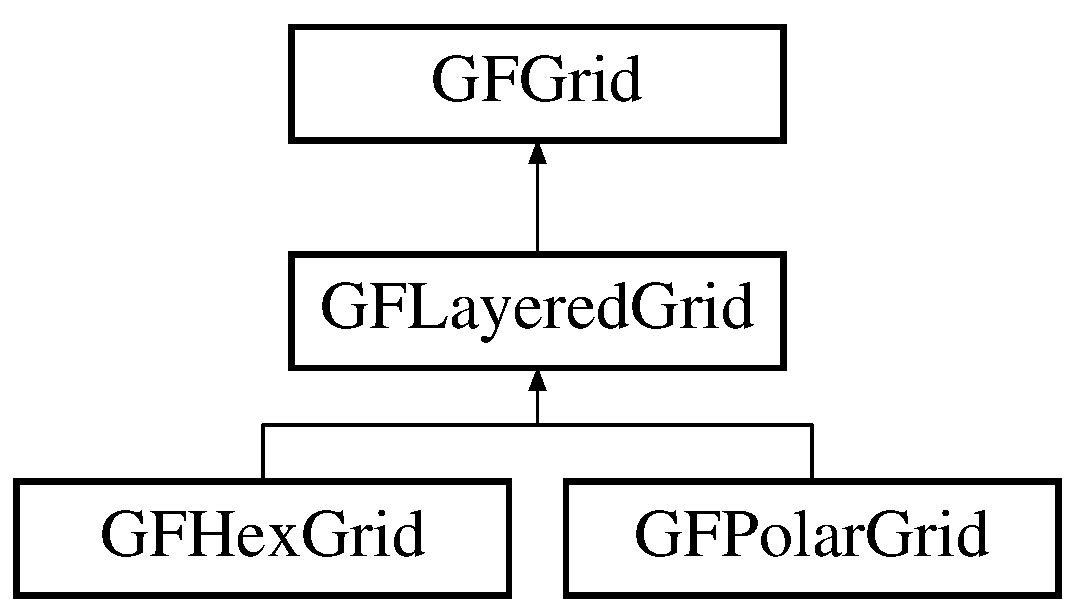
\includegraphics[height=3.000000cm]{class_g_f_layered_grid}
\end{center}
\end{figure}
\subsection*{Public Member Functions}
\begin{DoxyCompactItemize}
\item 
override Vector3 \hyperlink{class_g_f_layered_grid_a0fad538e6ffb56209e76da00c357a3c9_a0fad538e6ffb56209e76da00c357a3c9}{Nearest\+Face\+W} (Vector3 world\+Point, \hyperlink{namespace_grid_framework_aa55de93079e09bd55c4cb660025820d5_aa55de93079e09bd55c4cb660025820d5}{Grid\+Plane} plane, bool do\+Debug)
\begin{DoxyCompactList}\small\item\em Returns the world position of the nearest face.\end{DoxyCompactList}\item 
override Vector3 \hyperlink{class_g_f_layered_grid_a5af848e6ee44af68a8c4748716925468_a5af848e6ee44af68a8c4748716925468}{Nearest\+Face\+G} (Vector3 world\+Point, \hyperlink{namespace_grid_framework_aa55de93079e09bd55c4cb660025820d5_aa55de93079e09bd55c4cb660025820d5}{Grid\+Plane} plane)
\begin{DoxyCompactList}\small\item\em Returns the grid position of the nearest Face.\end{DoxyCompactList}\end{DoxyCompactItemize}
\subsection*{Properties}
\begin{DoxyCompactItemize}
\item 
float \hyperlink{class_g_f_layered_grid_a3ff168354ca75d04aae2340c48c7070c_a3ff168354ca75d04aae2340c48c7070c}{depth}\hspace{0.3cm}{\ttfamily  \mbox{[}get, set\mbox{]}}
\begin{DoxyCompactList}\small\item\em How far apart layers of the grid are.\end{DoxyCompactList}\item 
\hyperlink{namespace_grid_framework_aa55de93079e09bd55c4cb660025820d5_aa55de93079e09bd55c4cb660025820d5}{Grid\+Plane} \hyperlink{class_g_f_layered_grid_aeda8ad1af2b0d4ed12481de40ddb3f55_aeda8ad1af2b0d4ed12481de40ddb3f55}{grid\+Plane}\hspace{0.3cm}{\ttfamily  \mbox{[}get, set\mbox{]}}
\begin{DoxyCompactList}\small\item\em What plane the layers are on.\end{DoxyCompactList}\end{DoxyCompactItemize}
\subsection*{Additional Inherited Members}


\subsection{Detailed Description}
This class serves as a parent for all grids composed out of two-\/dimensional grids stacked on top of each other (currently only hex-\/ and polar grids). These grids have a plane (orientation) and a \char`\"{}depth\char`\"{} (how densely stacked they are). Other than keeping common values and internal methods in one place, this class has not much practical use. I recommend yu ignore it, it is documented just for the sake of completion. 

\subsection{Member Function Documentation}
\hypertarget{class_g_f_layered_grid_a5af848e6ee44af68a8c4748716925468_a5af848e6ee44af68a8c4748716925468}{\index{G\+F\+Layered\+Grid@{G\+F\+Layered\+Grid}!Nearest\+Face\+G@{Nearest\+Face\+G}}
\index{Nearest\+Face\+G@{Nearest\+Face\+G}!G\+F\+Layered\+Grid@{G\+F\+Layered\+Grid}}
\subsubsection[{Nearest\+Face\+G}]{\setlength{\rightskip}{0pt plus 5cm}override Vector3 G\+F\+Layered\+Grid.\+Nearest\+Face\+G (
\begin{DoxyParamCaption}
\item[{Vector3}]{world\+Point, }
\item[{{\bf Grid\+Plane}}]{plane}
\end{DoxyParamCaption}
)\hspace{0.3cm}{\ttfamily [virtual]}}}\label{class_g_f_layered_grid_a5af848e6ee44af68a8c4748716925468_a5af848e6ee44af68a8c4748716925468}
\begin{DoxyReturn}{Returns}
Grid position of the nearest face.
\end{DoxyReturn}

\begin{DoxyParams}{Parameters}
{\em world\+Point} & Point in world space.\\
\hline
{\em plane} & Plane on which the face lies.\\
\hline
\end{DoxyParams}


Similar to \hyperlink{class_g_f_grid_a7eaa2821cf118bb4821bd2cbf40029da_a7eaa2821cf118bb4821bd2cbf40029da}{Nearest\+Vertex\+G}, it returns the grid coordinates of a face on the grid. Since the face is enclosed by several vertices, the returned value is the point in between all of the vertices. You also need to specify on which plane the face lies (optional for hex-\/ and polar grids).

This is just an abstract template for the method, look into the specific class for exact implementation. 

Implements \hyperlink{class_g_f_grid_aac129f3df1da5cdbc31143ecc7db35d2_aac129f3df1da5cdbc31143ecc7db35d2}{G\+F\+Grid}.

\hypertarget{class_g_f_layered_grid_a0fad538e6ffb56209e76da00c357a3c9_a0fad538e6ffb56209e76da00c357a3c9}{\index{G\+F\+Layered\+Grid@{G\+F\+Layered\+Grid}!Nearest\+Face\+W@{Nearest\+Face\+W}}
\index{Nearest\+Face\+W@{Nearest\+Face\+W}!G\+F\+Layered\+Grid@{G\+F\+Layered\+Grid}}
\subsubsection[{Nearest\+Face\+W}]{\setlength{\rightskip}{0pt plus 5cm}override Vector3 G\+F\+Layered\+Grid.\+Nearest\+Face\+W (
\begin{DoxyParamCaption}
\item[{Vector3}]{world\+Point, }
\item[{{\bf Grid\+Plane}}]{plane, }
\item[{bool}]{do\+Debug}
\end{DoxyParamCaption}
)\hspace{0.3cm}{\ttfamily [virtual]}}}\label{class_g_f_layered_grid_a0fad538e6ffb56209e76da00c357a3c9_a0fad538e6ffb56209e76da00c357a3c9}
\begin{DoxyReturn}{Returns}
World position of the nearest face.
\end{DoxyReturn}

\begin{DoxyParams}{Parameters}
{\em world\+Point} & Point in world space.\\
\hline
{\em plane} & Plane on which the face lies.\\
\hline
{\em do\+Debug} & If set to {\ttfamily true} draw a sphere at the destination.\\
\hline
\end{DoxyParams}


Similar to \hyperlink{class_g_f_grid_a5865880fa767bf5562301bca419b8bb9_a5865880fa767bf5562301bca419b8bb9}{Nearest\+Vertex\+W}, it returns the world coordinates of a face on the grid. Since the face is enclosed by several vertices, the returned value is the point in between all of the vertices. You also need to specify on which plane the face lies (optional for hex-\/ and polar grids). If {\itshape do\+Debug}  is set a small gizmo face will drawn there.

This is just an abstract template for the method, look into the specific class for exact implementation. 

Implements \hyperlink{class_g_f_grid_ae8711b08c90871f6e88800a30ff5077f_ae8711b08c90871f6e88800a30ff5077f}{G\+F\+Grid}.



\subsection{Property Documentation}
\hypertarget{class_g_f_layered_grid_a3ff168354ca75d04aae2340c48c7070c_a3ff168354ca75d04aae2340c48c7070c}{\index{G\+F\+Layered\+Grid@{G\+F\+Layered\+Grid}!depth@{depth}}
\index{depth@{depth}!G\+F\+Layered\+Grid@{G\+F\+Layered\+Grid}}
\subsubsection[{depth}]{\setlength{\rightskip}{0pt plus 5cm}float G\+F\+Layered\+Grid.\+depth\hspace{0.3cm}{\ttfamily [get]}, {\ttfamily [set]}}}\label{class_g_f_layered_grid_a3ff168354ca75d04aae2340c48c7070c_a3ff168354ca75d04aae2340c48c7070c}
Depth of grid layers.

Layered grids are made of an infinite number of two-\/dimensional grids stacked on top of each other. This determines how far apart those layers are. The value cannot be lower than 0.\+1 in order to prevent contradictory values. \hypertarget{class_g_f_layered_grid_aeda8ad1af2b0d4ed12481de40ddb3f55_aeda8ad1af2b0d4ed12481de40ddb3f55}{\index{G\+F\+Layered\+Grid@{G\+F\+Layered\+Grid}!grid\+Plane@{grid\+Plane}}
\index{grid\+Plane@{grid\+Plane}!G\+F\+Layered\+Grid@{G\+F\+Layered\+Grid}}
\subsubsection[{grid\+Plane}]{\setlength{\rightskip}{0pt plus 5cm}{\bf Grid\+Plane} G\+F\+Layered\+Grid.\+grid\+Plane\hspace{0.3cm}{\ttfamily [get]}, {\ttfamily [set]}}}\label{class_g_f_layered_grid_aeda8ad1af2b0d4ed12481de40ddb3f55_aeda8ad1af2b0d4ed12481de40ddb3f55}
The plane on which the grid is aligned.

Layered grids are made of an infinite number of two-\/dimensional grids stacked on top of each other. This determines the orientation of these layers, i. e. if they are X\+Y-\/, X\+Z-\/ or Y\+Z-\/layers. 

The documentation for this class was generated from the following file\+:\begin{DoxyCompactItemize}
\item 
G\+F\+Layered\+Grid.\+cs\end{DoxyCompactItemize}

\hypertarget{class_g_f_polar_grid}{\section{G\+F\+Polar\+Grid Class Reference}
\label{class_g_f_polar_grid}\index{G\+F\+Polar\+Grid@{G\+F\+Polar\+Grid}}
}


A polar grid based on cylindrical coordinates. 


Inheritance diagram for G\+F\+Polar\+Grid\+:\begin{figure}[H]
\begin{center}
\leavevmode
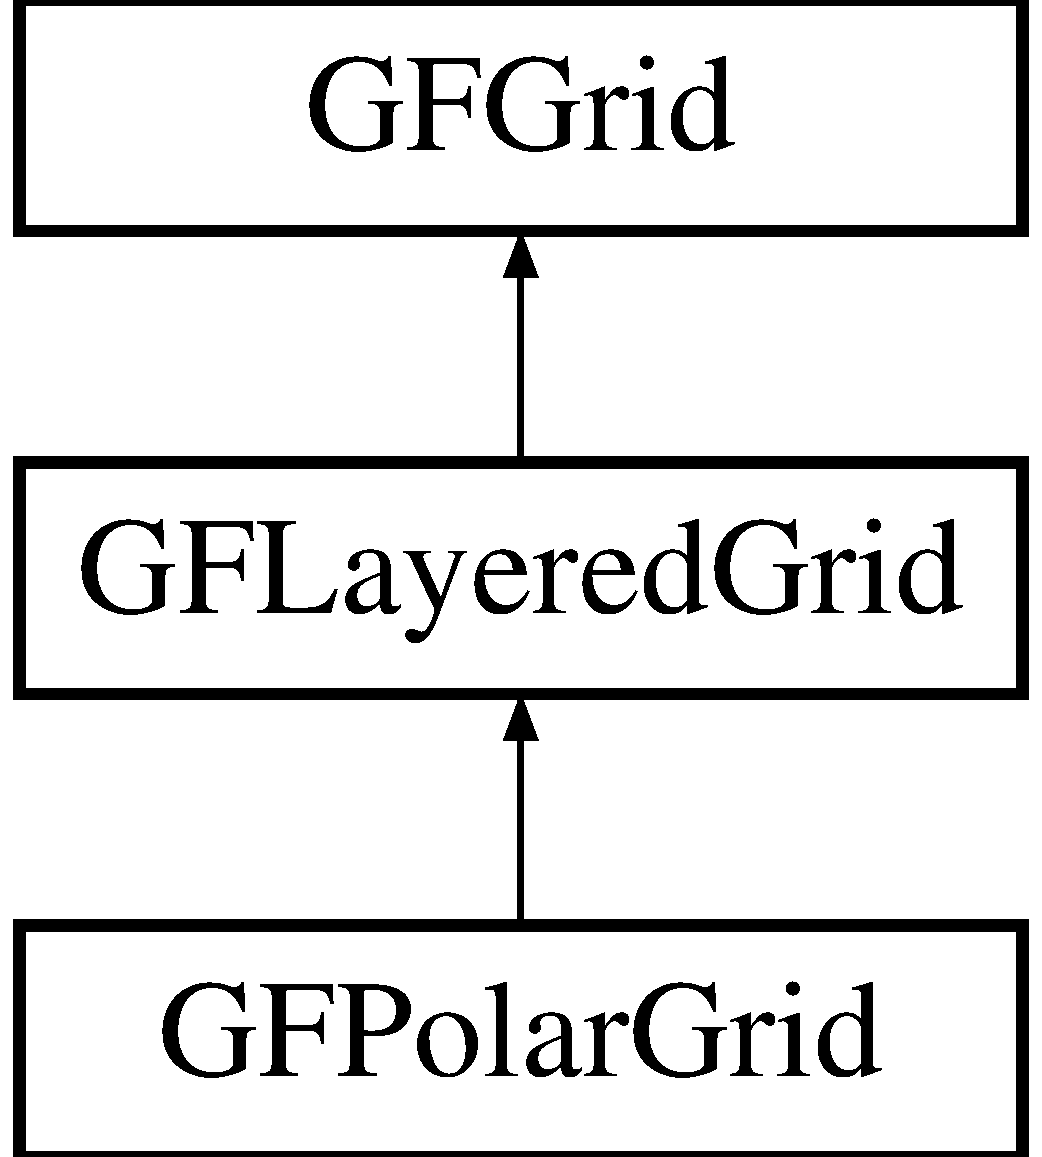
\includegraphics[height=3.000000cm]{class_g_f_polar_grid}
\end{center}
\end{figure}
\subsection*{Public Member Functions}
\begin{DoxyCompactItemize}
\item 
override Vector3 \hyperlink{class_g_f_polar_grid_a925bc4556e0c7422f476409b4f48067e_a925bc4556e0c7422f476409b4f48067e}{World\+To\+Grid} (Vector3 world\+Point)
\begin{DoxyCompactList}\small\item\em Converts from world to grid coordinates.\end{DoxyCompactList}\item 
override Vector3 \hyperlink{class_g_f_polar_grid_a80a4698250b08f212f3681abadbc5012_a80a4698250b08f212f3681abadbc5012}{Grid\+To\+World} (Vector3 grid\+Point)
\begin{DoxyCompactList}\small\item\em Converts from grid to world coordinates.\end{DoxyCompactList}\item 
Vector3 \hyperlink{class_g_f_polar_grid_a4fb1df768f7700590e23205e089dc58d_a4fb1df768f7700590e23205e089dc58d}{World\+To\+Polar} (Vector3 world\+Point)
\begin{DoxyCompactList}\small\item\em Converts from world to polar coordinates.\end{DoxyCompactList}\item 
Vector3 \hyperlink{class_g_f_polar_grid_a3dc57117173969cf60d3275e533a3ff8_a3dc57117173969cf60d3275e533a3ff8}{Polar\+To\+World} (Vector3 polar\+Point)
\begin{DoxyCompactList}\small\item\em Converts from polar to world coordinates.\end{DoxyCompactList}\item 
Vector3 \hyperlink{class_g_f_polar_grid_a2a571c5fc91475f86f7643f45fc1c265_a2a571c5fc91475f86f7643f45fc1c265}{Grid\+To\+Polar} (Vector3 grid\+Point)
\begin{DoxyCompactList}\small\item\em Converts a point from grid to polar space.\end{DoxyCompactList}\item 
Vector3 \hyperlink{class_g_f_polar_grid_a7e4ceb8cf00db2c36b74ef76ecaa2a15_a7e4ceb8cf00db2c36b74ef76ecaa2a15}{Polar\+To\+Grid} (Vector3 polar\+Point)
\begin{DoxyCompactList}\small\item\em Converts a point from polar to grid space.\end{DoxyCompactList}\item 
float \hyperlink{class_g_f_polar_grid_ab11007629046b75d7a788f65a952fdaf_ab11007629046b75d7a788f65a952fdaf}{Angle2\+Sector} (float \hyperlink{class_g_f_polar_grid_ad57e2dcf03806e576191953034dcd74c_ad57e2dcf03806e576191953034dcd74c}{angle}, \hyperlink{namespace_grid_framework_af11322a36c09698c9ad2fa65f85320a9_af11322a36c09698c9ad2fa65f85320a9}{Angle\+Mode} mode=Angle\+Mode.\+radians)
\begin{DoxyCompactList}\small\item\em Converts an angle (radians or degree) to the corresponding sector coordinate.\end{DoxyCompactList}\item 
float \hyperlink{class_g_f_polar_grid_a675288b8c01f479b18411bb31c8d05eb_a675288b8c01f479b18411bb31c8d05eb}{Sector2\+Angle} (float sector, \hyperlink{namespace_grid_framework_af11322a36c09698c9ad2fa65f85320a9_af11322a36c09698c9ad2fa65f85320a9}{Angle\+Mode} mode=Angle\+Mode.\+radians)
\begin{DoxyCompactList}\small\item\em Converts a sector to the corresponding angle coordinate (radians or degree).\end{DoxyCompactList}\item 
Quaternion \hyperlink{class_g_f_polar_grid_a36467502f91e0fc6ca2247f2ce72ddaa_a36467502f91e0fc6ca2247f2ce72ddaa}{Angle2\+Rotation} (float \hyperlink{class_g_f_polar_grid_ad57e2dcf03806e576191953034dcd74c_ad57e2dcf03806e576191953034dcd74c}{angle}, \hyperlink{namespace_grid_framework_af11322a36c09698c9ad2fa65f85320a9_af11322a36c09698c9ad2fa65f85320a9}{Angle\+Mode} mode=Angle\+Mode.\+radians)
\begin{DoxyCompactList}\small\item\em Converts an angle around the origin to a rotation.\end{DoxyCompactList}\item 
Quaternion \hyperlink{class_g_f_polar_grid_a7cf5d37fe48331dc630dfedaf585e2e0_a7cf5d37fe48331dc630dfedaf585e2e0}{Sector2\+Rotation} (float sector)
\begin{DoxyCompactList}\small\item\em Converts a sector around the origin to a rotation.\end{DoxyCompactList}\item 
Quaternion \hyperlink{class_g_f_polar_grid_a7d03e8c0b4ec132f58c587539e0027c7_a7d03e8c0b4ec132f58c587539e0027c7}{World2\+Rotation} (Vector3 world\+Point)
\begin{DoxyCompactList}\small\item\em Converts a world position to a rotation around the origin.\end{DoxyCompactList}\item 
float \hyperlink{class_g_f_polar_grid_a4ae9f55612e4c91a5d28b27c924c7432_a4ae9f55612e4c91a5d28b27c924c7432}{World2\+Angle} (Vector3 world\+Point, \hyperlink{namespace_grid_framework_af11322a36c09698c9ad2fa65f85320a9_af11322a36c09698c9ad2fa65f85320a9}{Angle\+Mode} mode=Angle\+Mode.\+radians)
\begin{DoxyCompactList}\small\item\em Converts a world position to an angle around the origin.\end{DoxyCompactList}\item 
float \hyperlink{class_g_f_polar_grid_aa03b782920133982d3ceec6169c2fa08_aa03b782920133982d3ceec6169c2fa08}{World2\+Sector} (Vector3 world\+Point)
\begin{DoxyCompactList}\small\item\em Converts a world position to the sector of the grid it is in.\end{DoxyCompactList}\item 
float \hyperlink{class_g_f_polar_grid_a0c865b865e3dd5a5377f7f24c59ef33d_a0c865b865e3dd5a5377f7f24c59ef33d}{World2\+Radius} (Vector3 world\+Point)
\begin{DoxyCompactList}\small\item\em Converts a world position to the radius from the origin.\end{DoxyCompactList}\item 
override Vector3 \hyperlink{class_g_f_polar_grid_ab0fd04140a3de44e0b407629dcf0e124_ab0fd04140a3de44e0b407629dcf0e124}{Nearest\+Vertex\+W} (Vector3 world\+Point, bool do\+Debug)
\begin{DoxyCompactList}\small\item\em Returns the world position of the nearest vertex.\end{DoxyCompactList}\item 
override Vector3 \hyperlink{class_g_f_polar_grid_a96c9b87b860cfb9099079f6ae1c415d5_a96c9b87b860cfb9099079f6ae1c415d5}{Nearest\+Face\+W} (Vector3 world, bool do\+Debug)
\begin{DoxyCompactList}\small\item\em Returns the world position of the nearest face.\end{DoxyCompactList}\item 
override Vector3 \hyperlink{class_g_f_polar_grid_aa8d60db8cd64b7dbe083d380110ab9d9_aa8d60db8cd64b7dbe083d380110ab9d9}{Nearest\+Box\+W} (Vector3 world\+Point, bool do\+Debug)
\begin{DoxyCompactList}\small\item\em Returns the world position of the nearest box.\end{DoxyCompactList}\item 
override Vector3 \hyperlink{class_g_f_polar_grid_aa119074284b649c45ee9b1bb80153d4d_aa119074284b649c45ee9b1bb80153d4d}{Nearest\+Vertex\+G} (Vector3 world\+Point)
\begin{DoxyCompactList}\small\item\em Returns the grid position of the nearest vertex.\end{DoxyCompactList}\item 
override Vector3 \hyperlink{class_g_f_polar_grid_a14f3e5fe0e7db4b49bae10a146a9e5f6_a14f3e5fe0e7db4b49bae10a146a9e5f6}{Nearest\+Face\+G} (Vector3 world)
\begin{DoxyCompactList}\small\item\em Returns the grid position of the nearest Face.\end{DoxyCompactList}\item 
override Vector3 \hyperlink{class_g_f_polar_grid_abdc5c38b32d8fe3d6610127b54b89093_abdc5c38b32d8fe3d6610127b54b89093}{Nearest\+Box\+G} (Vector3 world\+Point)
\begin{DoxyCompactList}\small\item\em Returns the grid position of the nearest box.\end{DoxyCompactList}\item 
Vector3 \hyperlink{class_g_f_polar_grid_a267e38d14acaffe3e98bac47c75eb52d_a267e38d14acaffe3e98bac47c75eb52d}{Nearest\+Vertex\+P} (Vector3 world\+Point)
\begin{DoxyCompactList}\small\item\em Returns the grid position of the nearest vertex.\end{DoxyCompactList}\item 
Vector3 \hyperlink{class_g_f_polar_grid_a2d1331fb80b8029fe7c06c72c4a16077_a2d1331fb80b8029fe7c06c72c4a16077}{Nearest\+Face\+P} (Vector3 world\+Point)
\begin{DoxyCompactList}\small\item\em Returns the polar position of the nearest Face.\end{DoxyCompactList}\item 
Vector3 \hyperlink{class_g_f_polar_grid_a06654388a9f53f5e56971f7c8b7f40ad_a06654388a9f53f5e56971f7c8b7f40ad}{Nearest\+Box\+P} (Vector3 world\+Point)
\begin{DoxyCompactList}\small\item\em Returns the polar position of the nearest box.\end{DoxyCompactList}\item 
void \hyperlink{class_g_f_polar_grid_a14f45c2312bfe475e588d128dc108b0c_a14f45c2312bfe475e588d128dc108b0c}{Align\+Rotate\+Transform} (Transform transform, \hyperlink{class_grid_framework_1_1_vectors_1_1_bool_vector3}{Bool\+Vector3} lock\+Axis)
\begin{DoxyCompactList}\small\item\em Aligns and rotates a Transform.\end{DoxyCompactList}\item 
void \hyperlink{class_g_f_polar_grid_ad8054ff4516cc6929b110de4c2b0c77c_ad8054ff4516cc6929b110de4c2b0c77c}{Align\+Rotate\+Transform} (Transform the\+Transform)
\item 
override Vector3 \hyperlink{class_g_f_polar_grid_a5faa2b607e1ffc4ad2d3d5e7d62bf611_a5faa2b607e1ffc4ad2d3d5e7d62bf611}{Align\+Vector3} (Vector3 pos, Vector3 scale, \hyperlink{class_grid_framework_1_1_vectors_1_1_bool_vector3}{Bool\+Vector3} ignore\+Axis)
\begin{DoxyCompactList}\small\item\em Fits a position vector into the grid.\end{DoxyCompactList}\item 
override Vector3 \hyperlink{class_g_f_polar_grid_aa7d26ab4a4cfbe914001c7f635ee2ace_aa7d26ab4a4cfbe914001c7f635ee2ace}{Scale\+Vector3} (Vector3 scl, \hyperlink{class_grid_framework_1_1_vectors_1_1_bool_vector3}{Bool\+Vector3} ignore\+Axis)
\begin{DoxyCompactList}\small\item\em Scales a size vector to fit inside a grid.\end{DoxyCompactList}\item 
override void \hyperlink{class_g_f_polar_grid_a5c3dd0e599e358379dc7c83f31e1dc5f_a5c3dd0e599e358379dc7c83f31e1dc5f}{Render\+Grid} (int width=0, Camera cam=null, Transform cam\+Transform=null)
\end{DoxyCompactItemize}
\subsection*{Properties}
\begin{DoxyCompactItemize}
\item 
override Vector3 \hyperlink{class_g_f_polar_grid_a851ff16bfbf1204a1ab0b1b4de3ceb35_a851ff16bfbf1204a1ab0b1b4de3ceb35}{size}\hspace{0.3cm}{\ttfamily  \mbox{[}get, set\mbox{]}}
\begin{DoxyCompactList}\small\item\em Overrides the size of \hyperlink{class_g_f_grid}{G\+F\+Grid} to make sure the angular coordinate is clamped appropriately between 0 and 2π (360°) or 0 and \hyperlink{class_g_f_polar_grid_a10ed1b65007dca14afb8fb6d22d36de0_a10ed1b65007dca14afb8fb6d22d36de0}{sectors}.\end{DoxyCompactList}\item 
override Vector3 \hyperlink{class_g_f_polar_grid_a9f4b9bcd687f29d56f4aafa74655e27b_a9f4b9bcd687f29d56f4aafa74655e27b}{render\+From}\hspace{0.3cm}{\ttfamily  \mbox{[}get, set\mbox{]}}
\begin{DoxyCompactList}\small\item\em Overrides the property of \hyperlink{class_g_f_grid}{G\+F\+Grid} to make sure that the radial value is positive and the angular value is wrapped around properly.\end{DoxyCompactList}\item 
override Vector3 \hyperlink{class_g_f_polar_grid_a81cc21991e689a1e74821d1f2870852e_a81cc21991e689a1e74821d1f2870852e}{render\+To}\hspace{0.3cm}{\ttfamily  \mbox{[}get, set\mbox{]}}
\begin{DoxyCompactList}\small\item\em Overrides the property of \hyperlink{class_g_f_grid}{G\+F\+Grid} to make sure that the angular value is wrapped around properly.\end{DoxyCompactList}\item 
float \hyperlink{class_g_f_polar_grid_a71bf429c8c2630684969db7f7483416a_a71bf429c8c2630684969db7f7483416a}{radius}\hspace{0.3cm}{\ttfamily  \mbox{[}get, set\mbox{]}}
\begin{DoxyCompactList}\small\item\em The radius of the inner-\/most circle of the grid.\end{DoxyCompactList}\item 
int \hyperlink{class_g_f_polar_grid_a10ed1b65007dca14afb8fb6d22d36de0_a10ed1b65007dca14afb8fb6d22d36de0}{sectors}\hspace{0.3cm}{\ttfamily  \mbox{[}get, set\mbox{]}}
\begin{DoxyCompactList}\small\item\em The amount of sectors per circle.\end{DoxyCompactList}\item 
int \hyperlink{class_g_f_polar_grid_a734237fa4e6ad811a84f36d6532ba9f9_a734237fa4e6ad811a84f36d6532ba9f9}{smoothness}\hspace{0.3cm}{\ttfamily  \mbox{[}get, set\mbox{]}}
\begin{DoxyCompactList}\small\item\em Divides the sectors to create a smoother look.\end{DoxyCompactList}\item 
float \hyperlink{class_g_f_polar_grid_ad57e2dcf03806e576191953034dcd74c_ad57e2dcf03806e576191953034dcd74c}{angle}\hspace{0.3cm}{\ttfamily  \mbox{[}get\mbox{]}}
\begin{DoxyCompactList}\small\item\em The angle of a sector in radians.\end{DoxyCompactList}\item 
float \hyperlink{class_g_f_polar_grid_a5c0e2072d09f3add6e4012b89ce8d21e_a5c0e2072d09f3add6e4012b89ce8d21e}{angle\+Deg}\hspace{0.3cm}{\ttfamily  \mbox{[}get\mbox{]}}
\begin{DoxyCompactList}\small\item\em The angle of a sector in degrees.\end{DoxyCompactList}\end{DoxyCompactItemize}
\subsection*{Additional Inherited Members}


\subsection{Detailed Description}
A grid based on cylindrical coordinates. The caracterizing values are \hyperlink{class_g_f_polar_grid_a71bf429c8c2630684969db7f7483416a_a71bf429c8c2630684969db7f7483416a}{radius}, \hyperlink{class_g_f_polar_grid_a10ed1b65007dca14afb8fb6d22d36de0_a10ed1b65007dca14afb8fb6d22d36de0}{sectors} and \hyperlink{class_g_f_layered_grid_a3ff168354ca75d04aae2340c48c7070c_a3ff168354ca75d04aae2340c48c7070c}{depth}. The angle values are derived from \hyperlink{class_g_f_polar_grid_a10ed1b65007dca14afb8fb6d22d36de0_a10ed1b65007dca14afb8fb6d22d36de0}{sectors} and we use radians internally. The coordinate systems used are either a grid-\/based coordinate system based on the defining values or a regular cylindrical coordinate system. If you want polar coordinates just ignore the height component of the cylindrical coordinates.

It is important to note that the components of polar and grid coordinates represent the radius, radian angle and height. Which component represents what depends on the grid\+Plane. The user manual has a handy table for that purpose.

The members \hyperlink{class_g_f_polar_grid_a851ff16bfbf1204a1ab0b1b4de3ceb35_a851ff16bfbf1204a1ab0b1b4de3ceb35}{size}, \hyperlink{class_g_f_polar_grid_a9f4b9bcd687f29d56f4aafa74655e27b_a9f4b9bcd687f29d56f4aafa74655e27b}{render\+From} and \hyperlink{class_g_f_polar_grid_a81cc21991e689a1e74821d1f2870852e_a81cc21991e689a1e74821d1f2870852e}{render\+To} are inherited from \hyperlink{class_g_f_grid}{G\+F\+Grid}, but slightly different. The first component of all three cannot be lower than 0 and in the case of \hyperlink{class_g_f_polar_grid_a9f4b9bcd687f29d56f4aafa74655e27b_a9f4b9bcd687f29d56f4aafa74655e27b}{render\+From} it cannot be larger than the first component of {\ttfamily \hyperlink{class_g_f_polar_grid_a81cc21991e689a1e74821d1f2870852e_a81cc21991e689a1e74821d1f2870852e}{render\+To}}, and vice-\/versa. The second component is an angle in radians and wraps around as described in the user manual, no other restrictions. The third component is the height, it’s bounded from below by 0.\+01 and in the case of \hyperlink{class_g_f_polar_grid_a9f4b9bcd687f29d56f4aafa74655e27b_a9f4b9bcd687f29d56f4aafa74655e27b}{render\+From} it cannot be larger than \hyperlink{class_g_f_polar_grid_a81cc21991e689a1e74821d1f2870852e_a81cc21991e689a1e74821d1f2870852e}{render\+To} and vice-\/versa. 

\subsection{Member Function Documentation}
\hypertarget{class_g_f_polar_grid_a14f45c2312bfe475e588d128dc108b0c_a14f45c2312bfe475e588d128dc108b0c}{\index{G\+F\+Polar\+Grid@{G\+F\+Polar\+Grid}!Align\+Rotate\+Transform@{Align\+Rotate\+Transform}}
\index{Align\+Rotate\+Transform@{Align\+Rotate\+Transform}!G\+F\+Polar\+Grid@{G\+F\+Polar\+Grid}}
\subsubsection[{Align\+Rotate\+Transform}]{\setlength{\rightskip}{0pt plus 5cm}void G\+F\+Polar\+Grid.\+Align\+Rotate\+Transform (
\begin{DoxyParamCaption}
\item[{Transform}]{transform, }
\item[{{\bf Bool\+Vector3}}]{lock\+Axis}
\end{DoxyParamCaption}
)}}\label{class_g_f_polar_grid_a14f45c2312bfe475e588d128dc108b0c_a14f45c2312bfe475e588d128dc108b0c}

\begin{DoxyParams}{Parameters}
{\em transform} & The Transform to align.\\
\hline
{\em lock\+Axis} & Axis to ignore.\\
\hline
\end{DoxyParams}


Aligns a Transform and the rotates it depending on its position inside the grid. This method cobines two steps in one call for convenience. \hypertarget{class_g_f_polar_grid_ad8054ff4516cc6929b110de4c2b0c77c_ad8054ff4516cc6929b110de4c2b0c77c}{\index{G\+F\+Polar\+Grid@{G\+F\+Polar\+Grid}!Align\+Rotate\+Transform@{Align\+Rotate\+Transform}}
\index{Align\+Rotate\+Transform@{Align\+Rotate\+Transform}!G\+F\+Polar\+Grid@{G\+F\+Polar\+Grid}}
\subsubsection[{Align\+Rotate\+Transform}]{\setlength{\rightskip}{0pt plus 5cm}void G\+F\+Polar\+Grid.\+Align\+Rotate\+Transform (
\begin{DoxyParamCaption}
\item[{Transform}]{the\+Transform}
\end{DoxyParamCaption}
)}}\label{class_g_f_polar_grid_ad8054ff4516cc6929b110de4c2b0c77c_ad8054ff4516cc6929b110de4c2b0c77c}
This is an overloaded member function, provided for convenience. It differs from the above function only in what argument(s) it accepts. Use this overload when you want to appy the alignment on all axis, then you don't have to specity them. \hypertarget{class_g_f_polar_grid_a5faa2b607e1ffc4ad2d3d5e7d62bf611_a5faa2b607e1ffc4ad2d3d5e7d62bf611}{\index{G\+F\+Polar\+Grid@{G\+F\+Polar\+Grid}!Align\+Vector3@{Align\+Vector3}}
\index{Align\+Vector3@{Align\+Vector3}!G\+F\+Polar\+Grid@{G\+F\+Polar\+Grid}}
\subsubsection[{Align\+Vector3}]{\setlength{\rightskip}{0pt plus 5cm}override Vector3 G\+F\+Polar\+Grid.\+Align\+Vector3 (
\begin{DoxyParamCaption}
\item[{Vector3}]{pos, }
\item[{Vector3}]{scale, }
\item[{{\bf Bool\+Vector3}}]{ignore\+Axis}
\end{DoxyParamCaption}
)\hspace{0.3cm}{\ttfamily [virtual]}}}\label{class_g_f_polar_grid_a5faa2b607e1ffc4ad2d3d5e7d62bf611_a5faa2b607e1ffc4ad2d3d5e7d62bf611}

\begin{DoxyParams}{Parameters}
{\em pos} & The position to align.\\
\hline
{\em scale} & A simulated scale to decide how exactly to fit the poistion into the grid.\\
\hline
{\em ignore\+Axis} & Which axes should be ignored.\\
\hline
\end{DoxyParams}
\begin{DoxyReturn}{Returns}
Aligned position vector.
\end{DoxyReturn}


Fits a position inside the grid by using the object’s transform. Currently the object will snap either on edges or between, depending on which is closer, ignoring the {\itshape scale}  passed, but I might add an optionfor this in the future. 

Implements \hyperlink{class_g_f_grid_a18b3e57431dc0db8f651479e4fb04a8f_a18b3e57431dc0db8f651479e4fb04a8f}{G\+F\+Grid}.

\hypertarget{class_g_f_polar_grid_a36467502f91e0fc6ca2247f2ce72ddaa_a36467502f91e0fc6ca2247f2ce72ddaa}{\index{G\+F\+Polar\+Grid@{G\+F\+Polar\+Grid}!Angle2\+Rotation@{Angle2\+Rotation}}
\index{Angle2\+Rotation@{Angle2\+Rotation}!G\+F\+Polar\+Grid@{G\+F\+Polar\+Grid}}
\subsubsection[{Angle2\+Rotation}]{\setlength{\rightskip}{0pt plus 5cm}Quaternion G\+F\+Polar\+Grid.\+Angle2\+Rotation (
\begin{DoxyParamCaption}
\item[{float}]{angle, }
\item[{{\bf Angle\+Mode}}]{mode = {\ttfamily AngleMode.radians}}
\end{DoxyParamCaption}
)}}\label{class_g_f_polar_grid_a36467502f91e0fc6ca2247f2ce72ddaa_a36467502f91e0fc6ca2247f2ce72ddaa}
\begin{DoxyReturn}{Returns}
Rotation quaterion which rotates arround the origin by {\itshape angle} .
\end{DoxyReturn}

\begin{DoxyParams}{Parameters}
{\em angle} & Angle in either radians or degrees.\\
\hline
{\em mode} & The mode of the angle, defaults to radians.\\
\hline
\end{DoxyParams}


This method returns a quaternion which represents a rotation within the grid. The result is a combination of the grid's own rotation and the rotation from the angle. Since we use an angle, this method is more suitable for polar coordinates than grid coordinates. See \hyperlink{class_g_f_polar_grid_a7cf5d37fe48331dc630dfedaf585e2e0_a7cf5d37fe48331dc630dfedaf585e2e0}{Sector2\+Rotation} for a similar method that uses sectors. \hypertarget{class_g_f_polar_grid_ab11007629046b75d7a788f65a952fdaf_ab11007629046b75d7a788f65a952fdaf}{\index{G\+F\+Polar\+Grid@{G\+F\+Polar\+Grid}!Angle2\+Sector@{Angle2\+Sector}}
\index{Angle2\+Sector@{Angle2\+Sector}!G\+F\+Polar\+Grid@{G\+F\+Polar\+Grid}}
\subsubsection[{Angle2\+Sector}]{\setlength{\rightskip}{0pt plus 5cm}float G\+F\+Polar\+Grid.\+Angle2\+Sector (
\begin{DoxyParamCaption}
\item[{float}]{angle, }
\item[{{\bf Angle\+Mode}}]{mode = {\ttfamily AngleMode.radians}}
\end{DoxyParamCaption}
)}}\label{class_g_f_polar_grid_ab11007629046b75d7a788f65a952fdaf_ab11007629046b75d7a788f65a952fdaf}
\begin{DoxyReturn}{Returns}
Sector value of the angle.
\end{DoxyReturn}

\begin{DoxyParams}{Parameters}
{\em angle} & Angle in either radians or degress.\\
\hline
{\em mode} & The mode of the angle, defaults to radians.\\
\hline
\end{DoxyParams}


This method takes in an angle and returns in which sector the angle lies. If the angle exceeds 2π or 360° it wraps around, nagetive angles are automatically subtracted from 2π or 360°.

Let's take a grid with six sectors for example, then one sector has an agle of 360° / 6 = 60°, so a 135° angle corresponds to a sector value of 130° / 60° = 2.\+25.\hypertarget{class_g_f_polar_grid_a2a571c5fc91475f86f7643f45fc1c265_a2a571c5fc91475f86f7643f45fc1c265}{\index{G\+F\+Polar\+Grid@{G\+F\+Polar\+Grid}!Grid\+To\+Polar@{Grid\+To\+Polar}}
\index{Grid\+To\+Polar@{Grid\+To\+Polar}!G\+F\+Polar\+Grid@{G\+F\+Polar\+Grid}}
\subsubsection[{Grid\+To\+Polar}]{\setlength{\rightskip}{0pt plus 5cm}Vector3 G\+F\+Polar\+Grid.\+Grid\+To\+Polar (
\begin{DoxyParamCaption}
\item[{Vector3}]{grid\+Point}
\end{DoxyParamCaption}
)}}\label{class_g_f_polar_grid_a2a571c5fc91475f86f7643f45fc1c265_a2a571c5fc91475f86f7643f45fc1c265}
\begin{DoxyReturn}{Returns}
Point in polar space.
\end{DoxyReturn}

\begin{DoxyParams}{Parameters}
{\em grid\+Point} & Point in grid space.\\
\hline
\end{DoxyParams}


Converts a point from grid to polar space. The main difference is that grid coordinates are dependent on the grid's parameters, while polar coordinates are not. \hypertarget{class_g_f_polar_grid_a80a4698250b08f212f3681abadbc5012_a80a4698250b08f212f3681abadbc5012}{\index{G\+F\+Polar\+Grid@{G\+F\+Polar\+Grid}!Grid\+To\+World@{Grid\+To\+World}}
\index{Grid\+To\+World@{Grid\+To\+World}!G\+F\+Polar\+Grid@{G\+F\+Polar\+Grid}}
\subsubsection[{Grid\+To\+World}]{\setlength{\rightskip}{0pt plus 5cm}override Vector3 G\+F\+Polar\+Grid.\+Grid\+To\+World (
\begin{DoxyParamCaption}
\item[{Vector3}]{grid\+Point}
\end{DoxyParamCaption}
)\hspace{0.3cm}{\ttfamily [virtual]}}}\label{class_g_f_polar_grid_a80a4698250b08f212f3681abadbc5012_a80a4698250b08f212f3681abadbc5012}
\begin{DoxyReturn}{Returns}
World coordinates of the grid point.
\end{DoxyReturn}

\begin{DoxyParams}{Parameters}
{\em grid\+Point} & Point in grid space.\\
\hline
\end{DoxyParams}


Converts a point from grid space to world space. 

Implements \hyperlink{class_g_f_grid_af32d7bfcecb5da3fdc47b972b551e33e_af32d7bfcecb5da3fdc47b972b551e33e}{G\+F\+Grid}.

\hypertarget{class_g_f_polar_grid_abdc5c38b32d8fe3d6610127b54b89093_abdc5c38b32d8fe3d6610127b54b89093}{\index{G\+F\+Polar\+Grid@{G\+F\+Polar\+Grid}!Nearest\+Box\+G@{Nearest\+Box\+G}}
\index{Nearest\+Box\+G@{Nearest\+Box\+G}!G\+F\+Polar\+Grid@{G\+F\+Polar\+Grid}}
\subsubsection[{Nearest\+Box\+G}]{\setlength{\rightskip}{0pt plus 5cm}override Vector3 G\+F\+Polar\+Grid.\+Nearest\+Box\+G (
\begin{DoxyParamCaption}
\item[{Vector3}]{world\+Point}
\end{DoxyParamCaption}
)\hspace{0.3cm}{\ttfamily [virtual]}}}\label{class_g_f_polar_grid_abdc5c38b32d8fe3d6610127b54b89093_abdc5c38b32d8fe3d6610127b54b89093}
\begin{DoxyReturn}{Returns}
Grid position of the nearest box.
\end{DoxyReturn}

\begin{DoxyParams}{Parameters}
{\em world\+Point} & Point in world space.\\
\hline
\end{DoxyParams}


Similar to \hyperlink{class_g_f_polar_grid_aa119074284b649c45ee9b1bb80153d4d_aa119074284b649c45ee9b1bb80153d4d}{Nearest\+Vertex\+G}, it returns the grid coordinates of a box in the grid. Since the box is enclosed by several vertices, the returned value is the point in between all of the vertices. 

Implements \hyperlink{class_g_f_grid_adb7c70449b2449c1e82132e6300cc1a5_adb7c70449b2449c1e82132e6300cc1a5}{G\+F\+Grid}.

\hypertarget{class_g_f_polar_grid_a06654388a9f53f5e56971f7c8b7f40ad_a06654388a9f53f5e56971f7c8b7f40ad}{\index{G\+F\+Polar\+Grid@{G\+F\+Polar\+Grid}!Nearest\+Box\+P@{Nearest\+Box\+P}}
\index{Nearest\+Box\+P@{Nearest\+Box\+P}!G\+F\+Polar\+Grid@{G\+F\+Polar\+Grid}}
\subsubsection[{Nearest\+Box\+P}]{\setlength{\rightskip}{0pt plus 5cm}Vector3 G\+F\+Polar\+Grid.\+Nearest\+Box\+P (
\begin{DoxyParamCaption}
\item[{Vector3}]{world\+Point}
\end{DoxyParamCaption}
)}}\label{class_g_f_polar_grid_a06654388a9f53f5e56971f7c8b7f40ad_a06654388a9f53f5e56971f7c8b7f40ad}
\begin{DoxyReturn}{Returns}
Polar position of the nearest box.
\end{DoxyReturn}

\begin{DoxyParams}{Parameters}
{\em world\+Point} & Point in world space.\\
\hline
\end{DoxyParams}


Similar to \hyperlink{class_g_f_polar_grid_a267e38d14acaffe3e98bac47c75eb52d_a267e38d14acaffe3e98bac47c75eb52d}{Nearest\+Vertex\+P}, it returns the polar coordinates of a box in the grid. Since the box is enclosed by several vertices, the returned value is the point in between all of the vertices. \hypertarget{class_g_f_polar_grid_aa8d60db8cd64b7dbe083d380110ab9d9_aa8d60db8cd64b7dbe083d380110ab9d9}{\index{G\+F\+Polar\+Grid@{G\+F\+Polar\+Grid}!Nearest\+Box\+W@{Nearest\+Box\+W}}
\index{Nearest\+Box\+W@{Nearest\+Box\+W}!G\+F\+Polar\+Grid@{G\+F\+Polar\+Grid}}
\subsubsection[{Nearest\+Box\+W}]{\setlength{\rightskip}{0pt plus 5cm}override Vector3 G\+F\+Polar\+Grid.\+Nearest\+Box\+W (
\begin{DoxyParamCaption}
\item[{Vector3}]{world\+Point, }
\item[{bool}]{do\+Debug}
\end{DoxyParamCaption}
)\hspace{0.3cm}{\ttfamily [virtual]}}}\label{class_g_f_polar_grid_aa8d60db8cd64b7dbe083d380110ab9d9_aa8d60db8cd64b7dbe083d380110ab9d9}
\begin{DoxyReturn}{Returns}
World position of the nearest box.
\end{DoxyReturn}

\begin{DoxyParams}{Parameters}
{\em world\+Point} & Point in world space.\\
\hline
{\em do\+Debug} & If set to {\ttfamily true} draw a sphere at the destination.\\
\hline
\end{DoxyParams}


Similar to \hyperlink{class_g_f_polar_grid_ab0fd04140a3de44e0b407629dcf0e124_ab0fd04140a3de44e0b407629dcf0e124}{Nearest\+Vertex\+W}, it returns the world coordinates of a box in the grid. Since the box is enclosed by several vertices, the returned value is the point in between all of the vertices. If {\itshape do\+Debug}  is set a small gizmo box will drawn there. 

Implements \hyperlink{class_g_f_grid_a02fcf02269ca5a2064acccecde9819eb_a02fcf02269ca5a2064acccecde9819eb}{G\+F\+Grid}.

\hypertarget{class_g_f_polar_grid_a14f3e5fe0e7db4b49bae10a146a9e5f6_a14f3e5fe0e7db4b49bae10a146a9e5f6}{\index{G\+F\+Polar\+Grid@{G\+F\+Polar\+Grid}!Nearest\+Face\+G@{Nearest\+Face\+G}}
\index{Nearest\+Face\+G@{Nearest\+Face\+G}!G\+F\+Polar\+Grid@{G\+F\+Polar\+Grid}}
\subsubsection[{Nearest\+Face\+G}]{\setlength{\rightskip}{0pt plus 5cm}override Vector3 G\+F\+Polar\+Grid.\+Nearest\+Face\+G (
\begin{DoxyParamCaption}
\item[{Vector3}]{world}
\end{DoxyParamCaption}
)\hspace{0.3cm}{\ttfamily [virtual]}}}\label{class_g_f_polar_grid_a14f3e5fe0e7db4b49bae10a146a9e5f6_a14f3e5fe0e7db4b49bae10a146a9e5f6}
\begin{DoxyReturn}{Returns}
Grid position of the nearest face.
\end{DoxyReturn}

\begin{DoxyParams}{Parameters}
{\em world} & Point in world space.\\
\hline
\end{DoxyParams}


Similar to \hyperlink{class_g_f_polar_grid_aa119074284b649c45ee9b1bb80153d4d_aa119074284b649c45ee9b1bb80153d4d}{Nearest\+Vertex\+G}, it returns the grid coordinates of a face on the grid. Since the face is enclosed by several vertices, the returned value is the point in between all of the vertices. 

Implements \hyperlink{class_g_f_layered_grid}{G\+F\+Layered\+Grid}.

\hypertarget{class_g_f_polar_grid_a2d1331fb80b8029fe7c06c72c4a16077_a2d1331fb80b8029fe7c06c72c4a16077}{\index{G\+F\+Polar\+Grid@{G\+F\+Polar\+Grid}!Nearest\+Face\+P@{Nearest\+Face\+P}}
\index{Nearest\+Face\+P@{Nearest\+Face\+P}!G\+F\+Polar\+Grid@{G\+F\+Polar\+Grid}}
\subsubsection[{Nearest\+Face\+P}]{\setlength{\rightskip}{0pt plus 5cm}Vector3 G\+F\+Polar\+Grid.\+Nearest\+Face\+P (
\begin{DoxyParamCaption}
\item[{Vector3}]{world\+Point}
\end{DoxyParamCaption}
)}}\label{class_g_f_polar_grid_a2d1331fb80b8029fe7c06c72c4a16077_a2d1331fb80b8029fe7c06c72c4a16077}
\begin{DoxyReturn}{Returns}
Polar position of the nearest face.
\end{DoxyReturn}

\begin{DoxyParams}{Parameters}
{\em world\+Point} & Point in world space.\\
\hline
\end{DoxyParams}


Similar to \hyperlink{class_g_f_polar_grid_a267e38d14acaffe3e98bac47c75eb52d_a267e38d14acaffe3e98bac47c75eb52d}{Nearest\+Vertex\+P}, it returns the polar coordinates of a face on the grid. Since the face is enclosed by several vertices, the returned value is the point in between all of the vertices. \hypertarget{class_g_f_polar_grid_a96c9b87b860cfb9099079f6ae1c415d5_a96c9b87b860cfb9099079f6ae1c415d5}{\index{G\+F\+Polar\+Grid@{G\+F\+Polar\+Grid}!Nearest\+Face\+W@{Nearest\+Face\+W}}
\index{Nearest\+Face\+W@{Nearest\+Face\+W}!G\+F\+Polar\+Grid@{G\+F\+Polar\+Grid}}
\subsubsection[{Nearest\+Face\+W}]{\setlength{\rightskip}{0pt plus 5cm}override Vector3 G\+F\+Polar\+Grid.\+Nearest\+Face\+W (
\begin{DoxyParamCaption}
\item[{Vector3}]{world, }
\item[{bool}]{do\+Debug}
\end{DoxyParamCaption}
)\hspace{0.3cm}{\ttfamily [virtual]}}}\label{class_g_f_polar_grid_a96c9b87b860cfb9099079f6ae1c415d5_a96c9b87b860cfb9099079f6ae1c415d5}
\begin{DoxyReturn}{Returns}
World position of the nearest face.
\end{DoxyReturn}

\begin{DoxyParams}{Parameters}
{\em world} & Point in world space.\\
\hline
{\em do\+Debug} & If set to {\ttfamily true} draw a sphere at the destination.\\
\hline
\end{DoxyParams}


Similar to \hyperlink{class_g_f_polar_grid_ab0fd04140a3de44e0b407629dcf0e124_ab0fd04140a3de44e0b407629dcf0e124}{Nearest\+Vertex\+W}, it returns the world coordinates of a face on the grid. Since the face is enclosed by several vertices, the returned value is the point in between all of the vertices. If {\itshape do\+Debug}  is set a small gizmo face will drawn there. 

Implements \hyperlink{class_g_f_layered_grid}{G\+F\+Layered\+Grid}.

\hypertarget{class_g_f_polar_grid_aa119074284b649c45ee9b1bb80153d4d_aa119074284b649c45ee9b1bb80153d4d}{\index{G\+F\+Polar\+Grid@{G\+F\+Polar\+Grid}!Nearest\+Vertex\+G@{Nearest\+Vertex\+G}}
\index{Nearest\+Vertex\+G@{Nearest\+Vertex\+G}!G\+F\+Polar\+Grid@{G\+F\+Polar\+Grid}}
\subsubsection[{Nearest\+Vertex\+G}]{\setlength{\rightskip}{0pt plus 5cm}override Vector3 G\+F\+Polar\+Grid.\+Nearest\+Vertex\+G (
\begin{DoxyParamCaption}
\item[{Vector3}]{world\+Point}
\end{DoxyParamCaption}
)\hspace{0.3cm}{\ttfamily [virtual]}}}\label{class_g_f_polar_grid_aa119074284b649c45ee9b1bb80153d4d_aa119074284b649c45ee9b1bb80153d4d}
\begin{DoxyReturn}{Returns}
Grid position of the nearest vertex.
\end{DoxyReturn}

\begin{DoxyParams}{Parameters}
{\em world\+Point} & Point in world space.\\
\hline
\end{DoxyParams}


Returns the position of the nerest vertex in grid coordinates from a given point in world space. 

Implements \hyperlink{class_g_f_grid_a7eaa2821cf118bb4821bd2cbf40029da_a7eaa2821cf118bb4821bd2cbf40029da}{G\+F\+Grid}.

\hypertarget{class_g_f_polar_grid_a267e38d14acaffe3e98bac47c75eb52d_a267e38d14acaffe3e98bac47c75eb52d}{\index{G\+F\+Polar\+Grid@{G\+F\+Polar\+Grid}!Nearest\+Vertex\+P@{Nearest\+Vertex\+P}}
\index{Nearest\+Vertex\+P@{Nearest\+Vertex\+P}!G\+F\+Polar\+Grid@{G\+F\+Polar\+Grid}}
\subsubsection[{Nearest\+Vertex\+P}]{\setlength{\rightskip}{0pt plus 5cm}Vector3 G\+F\+Polar\+Grid.\+Nearest\+Vertex\+P (
\begin{DoxyParamCaption}
\item[{Vector3}]{world\+Point}
\end{DoxyParamCaption}
)}}\label{class_g_f_polar_grid_a267e38d14acaffe3e98bac47c75eb52d_a267e38d14acaffe3e98bac47c75eb52d}
\begin{DoxyReturn}{Returns}
Polar position of the nearest vertex.
\end{DoxyReturn}

\begin{DoxyParams}{Parameters}
{\em world\+Point} & Point in world space.\\
\hline
\end{DoxyParams}


Returns the position of the nerest vertex in polar coordinates from a given point in world space. \hypertarget{class_g_f_polar_grid_ab0fd04140a3de44e0b407629dcf0e124_ab0fd04140a3de44e0b407629dcf0e124}{\index{G\+F\+Polar\+Grid@{G\+F\+Polar\+Grid}!Nearest\+Vertex\+W@{Nearest\+Vertex\+W}}
\index{Nearest\+Vertex\+W@{Nearest\+Vertex\+W}!G\+F\+Polar\+Grid@{G\+F\+Polar\+Grid}}
\subsubsection[{Nearest\+Vertex\+W}]{\setlength{\rightskip}{0pt plus 5cm}override Vector3 G\+F\+Polar\+Grid.\+Nearest\+Vertex\+W (
\begin{DoxyParamCaption}
\item[{Vector3}]{world\+Point, }
\item[{bool}]{do\+Debug}
\end{DoxyParamCaption}
)\hspace{0.3cm}{\ttfamily [virtual]}}}\label{class_g_f_polar_grid_ab0fd04140a3de44e0b407629dcf0e124_ab0fd04140a3de44e0b407629dcf0e124}
\begin{DoxyReturn}{Returns}
World position of the nearest vertex.
\end{DoxyReturn}

\begin{DoxyParams}{Parameters}
{\em world\+Point} & Point in world space.\\
\hline
{\em do\+Debug} & If set to {\ttfamily true} do debug.\\
\hline
\end{DoxyParams}


Returns the world position of the nearest vertex from a given point in world space. If {\itshape do\+Debug}  is set a small gizmo sphere will be drawn at that position. 

Implements \hyperlink{class_g_f_grid_a5865880fa767bf5562301bca419b8bb9_a5865880fa767bf5562301bca419b8bb9}{G\+F\+Grid}.

\hypertarget{class_g_f_polar_grid_a7e4ceb8cf00db2c36b74ef76ecaa2a15_a7e4ceb8cf00db2c36b74ef76ecaa2a15}{\index{G\+F\+Polar\+Grid@{G\+F\+Polar\+Grid}!Polar\+To\+Grid@{Polar\+To\+Grid}}
\index{Polar\+To\+Grid@{Polar\+To\+Grid}!G\+F\+Polar\+Grid@{G\+F\+Polar\+Grid}}
\subsubsection[{Polar\+To\+Grid}]{\setlength{\rightskip}{0pt plus 5cm}Vector3 G\+F\+Polar\+Grid.\+Polar\+To\+Grid (
\begin{DoxyParamCaption}
\item[{Vector3}]{polar\+Point}
\end{DoxyParamCaption}
)}}\label{class_g_f_polar_grid_a7e4ceb8cf00db2c36b74ef76ecaa2a15_a7e4ceb8cf00db2c36b74ef76ecaa2a15}
\begin{DoxyReturn}{Returns}
Point in grid space.
\end{DoxyReturn}

\begin{DoxyParams}{Parameters}
{\em polar\+Point} & Point in polar space.\\
\hline
\end{DoxyParams}


Converts a point from polar to grid space. The main difference is that grid coordinates are dependent on the grid's parameters, while polar coordinates are not. \hypertarget{class_g_f_polar_grid_a3dc57117173969cf60d3275e533a3ff8_a3dc57117173969cf60d3275e533a3ff8}{\index{G\+F\+Polar\+Grid@{G\+F\+Polar\+Grid}!Polar\+To\+World@{Polar\+To\+World}}
\index{Polar\+To\+World@{Polar\+To\+World}!G\+F\+Polar\+Grid@{G\+F\+Polar\+Grid}}
\subsubsection[{Polar\+To\+World}]{\setlength{\rightskip}{0pt plus 5cm}Vector3 G\+F\+Polar\+Grid.\+Polar\+To\+World (
\begin{DoxyParamCaption}
\item[{Vector3}]{polar\+Point}
\end{DoxyParamCaption}
)}}\label{class_g_f_polar_grid_a3dc57117173969cf60d3275e533a3ff8_a3dc57117173969cf60d3275e533a3ff8}
\begin{DoxyReturn}{Returns}
Point in world space.
\end{DoxyReturn}

\begin{DoxyParams}{Parameters}
{\em polar\+Point} & Point in polar space.\\
\hline
\end{DoxyParams}


Converts a point from polar space to world space. \hypertarget{class_g_f_polar_grid_a5c3dd0e599e358379dc7c83f31e1dc5f_a5c3dd0e599e358379dc7c83f31e1dc5f}{\index{G\+F\+Polar\+Grid@{G\+F\+Polar\+Grid}!Render\+Grid@{Render\+Grid}}
\index{Render\+Grid@{Render\+Grid}!G\+F\+Polar\+Grid@{G\+F\+Polar\+Grid}}
\subsubsection[{Render\+Grid}]{\setlength{\rightskip}{0pt plus 5cm}override void G\+F\+Polar\+Grid.\+Render\+Grid (
\begin{DoxyParamCaption}
\item[{int}]{width = {\ttfamily 0}, }
\item[{Camera}]{cam = {\ttfamily null}, }
\item[{Transform}]{cam\+Transform = {\ttfamily null}}
\end{DoxyParamCaption}
)\hspace{0.3cm}{\ttfamily [virtual]}}}\label{class_g_f_polar_grid_a5c3dd0e599e358379dc7c83f31e1dc5f_a5c3dd0e599e358379dc7c83f31e1dc5f}
This is an overloaded member function, provided for convenience. It differs from the above function only in what argument(s) it accepts. Renders the grid using {\ttfamily \hyperlink{class_g_f_polar_grid_a851ff16bfbf1204a1ab0b1b4de3ceb35_a851ff16bfbf1204a1ab0b1b4de3ceb35}{size}} for lower and upper limits, equal to {\ttfamily Render\+Grid(-\/size, size, use\+Separate\+Render\+Color ? render\+Axis\+Colors \+: axis\+Colors, width, cam, cam\+Transform);} 

Reimplemented from \hyperlink{class_g_f_grid_a24008f73b2c2ce9d6a699d25df998055_a24008f73b2c2ce9d6a699d25df998055}{G\+F\+Grid}.

\hypertarget{class_g_f_polar_grid_aa7d26ab4a4cfbe914001c7f635ee2ace_aa7d26ab4a4cfbe914001c7f635ee2ace}{\index{G\+F\+Polar\+Grid@{G\+F\+Polar\+Grid}!Scale\+Vector3@{Scale\+Vector3}}
\index{Scale\+Vector3@{Scale\+Vector3}!G\+F\+Polar\+Grid@{G\+F\+Polar\+Grid}}
\subsubsection[{Scale\+Vector3}]{\setlength{\rightskip}{0pt plus 5cm}override Vector3 G\+F\+Polar\+Grid.\+Scale\+Vector3 (
\begin{DoxyParamCaption}
\item[{Vector3}]{scl, }
\item[{{\bf Bool\+Vector3}}]{ignore\+Axis}
\end{DoxyParamCaption}
)\hspace{0.3cm}{\ttfamily [virtual]}}}\label{class_g_f_polar_grid_aa7d26ab4a4cfbe914001c7f635ee2ace_aa7d26ab4a4cfbe914001c7f635ee2ace}

\begin{DoxyParams}{Parameters}
{\em scl} & The vector to scale.\\
\hline
{\em ignore\+Axis} & The axes to ignore.\\
\hline
\end{DoxyParams}
\begin{DoxyReturn}{Returns}
The re-\/scaled vector.
\end{DoxyReturn}


Scales a given scale vector to the nearest multiple of the grid’s radius and depth, but does not change its position. The parameter {\itshape ignore\+Axis}  makes the function not touch the corresponding coordinate. 

Implements \hyperlink{class_g_f_grid_a02b3cf14a1529355c51e0d3ea646b4f8_a02b3cf14a1529355c51e0d3ea646b4f8}{G\+F\+Grid}.

\hypertarget{class_g_f_polar_grid_a675288b8c01f479b18411bb31c8d05eb_a675288b8c01f479b18411bb31c8d05eb}{\index{G\+F\+Polar\+Grid@{G\+F\+Polar\+Grid}!Sector2\+Angle@{Sector2\+Angle}}
\index{Sector2\+Angle@{Sector2\+Angle}!G\+F\+Polar\+Grid@{G\+F\+Polar\+Grid}}
\subsubsection[{Sector2\+Angle}]{\setlength{\rightskip}{0pt plus 5cm}float G\+F\+Polar\+Grid.\+Sector2\+Angle (
\begin{DoxyParamCaption}
\item[{float}]{sector, }
\item[{{\bf Angle\+Mode}}]{mode = {\ttfamily AngleMode.radians}}
\end{DoxyParamCaption}
)}}\label{class_g_f_polar_grid_a675288b8c01f479b18411bb31c8d05eb_a675288b8c01f479b18411bb31c8d05eb}
\begin{DoxyReturn}{Returns}
Angle value of the sector.
\end{DoxyReturn}

\begin{DoxyParams}{Parameters}
{\em sector} & Sector number.\\
\hline
{\em mode} & The mode of the angle, defaults to radians.\\
\hline
\end{DoxyParams}


This method takes in a sector coordinate and returns the corresponding angle around the origin. If the sector exceeds the amount of sectors of the grid it wraps around, nagetive sctors are automatically subtracted from the maximum.

Let's take a grid with six sectors for example, then one sector has an agle of 360° / 6 = 60°, so a 2.\+25 sector corresponds to an angle of 2.\+25 $\ast$ 60° = 135°.\hypertarget{class_g_f_polar_grid_a7cf5d37fe48331dc630dfedaf585e2e0_a7cf5d37fe48331dc630dfedaf585e2e0}{\index{G\+F\+Polar\+Grid@{G\+F\+Polar\+Grid}!Sector2\+Rotation@{Sector2\+Rotation}}
\index{Sector2\+Rotation@{Sector2\+Rotation}!G\+F\+Polar\+Grid@{G\+F\+Polar\+Grid}}
\subsubsection[{Sector2\+Rotation}]{\setlength{\rightskip}{0pt plus 5cm}Quaternion G\+F\+Polar\+Grid.\+Sector2\+Rotation (
\begin{DoxyParamCaption}
\item[{float}]{sector}
\end{DoxyParamCaption}
)}}\label{class_g_f_polar_grid_a7cf5d37fe48331dc630dfedaf585e2e0_a7cf5d37fe48331dc630dfedaf585e2e0}
\begin{DoxyReturn}{Returns}
Rotation quaterion which rotates arround the origin.
\end{DoxyReturn}

\begin{DoxyParams}{Parameters}
{\em sector} & Sector coordinate inside the grid.\\
\hline
\end{DoxyParams}


This is basically the same as \hyperlink{class_g_f_polar_grid_a36467502f91e0fc6ca2247f2ce72ddaa_a36467502f91e0fc6ca2247f2ce72ddaa}{Angle2\+Rotation}, excpet with sectors, which makes this method more suitable for grid coordinates than polar coordinates. \hypertarget{class_g_f_polar_grid_a4ae9f55612e4c91a5d28b27c924c7432_a4ae9f55612e4c91a5d28b27c924c7432}{\index{G\+F\+Polar\+Grid@{G\+F\+Polar\+Grid}!World2\+Angle@{World2\+Angle}}
\index{World2\+Angle@{World2\+Angle}!G\+F\+Polar\+Grid@{G\+F\+Polar\+Grid}}
\subsubsection[{World2\+Angle}]{\setlength{\rightskip}{0pt plus 5cm}float G\+F\+Polar\+Grid.\+World2\+Angle (
\begin{DoxyParamCaption}
\item[{Vector3}]{world\+Point, }
\item[{{\bf Angle\+Mode}}]{mode = {\ttfamily AngleMode.radians}}
\end{DoxyParamCaption}
)}}\label{class_g_f_polar_grid_a4ae9f55612e4c91a5d28b27c924c7432_a4ae9f55612e4c91a5d28b27c924c7432}
\begin{DoxyReturn}{Returns}
Angle between the point and the grid's \char`\"{}right\char`\"{} axis.
\end{DoxyReturn}

\begin{DoxyParams}{Parameters}
{\em world\+Point} & Point in world space.\\
\hline
{\em mode} & The mode of the angle, defaults to radians.\\
\hline
\end{DoxyParams}


This method returns which angle around the grid a given point in world space has. \hypertarget{class_g_f_polar_grid_a0c865b865e3dd5a5377f7f24c59ef33d_a0c865b865e3dd5a5377f7f24c59ef33d}{\index{G\+F\+Polar\+Grid@{G\+F\+Polar\+Grid}!World2\+Radius@{World2\+Radius}}
\index{World2\+Radius@{World2\+Radius}!G\+F\+Polar\+Grid@{G\+F\+Polar\+Grid}}
\subsubsection[{World2\+Radius}]{\setlength{\rightskip}{0pt plus 5cm}float G\+F\+Polar\+Grid.\+World2\+Radius (
\begin{DoxyParamCaption}
\item[{Vector3}]{world\+Point}
\end{DoxyParamCaption}
)}}\label{class_g_f_polar_grid_a0c865b865e3dd5a5377f7f24c59ef33d_a0c865b865e3dd5a5377f7f24c59ef33d}
\begin{DoxyReturn}{Returns}
Radius of the point from the grid.
\end{DoxyReturn}

\begin{DoxyParams}{Parameters}
{\em world\+Point} & Point in world space.\\
\hline
\end{DoxyParams}


This method returns the distance of a world point from the grid's radial axis. This is not the same as the point's distance from the grid's origin, because it doesn't take \char`\"{}height\char`\"{} into account. Thus it is always less or equal than the distance from the origin. \hypertarget{class_g_f_polar_grid_a7d03e8c0b4ec132f58c587539e0027c7_a7d03e8c0b4ec132f58c587539e0027c7}{\index{G\+F\+Polar\+Grid@{G\+F\+Polar\+Grid}!World2\+Rotation@{World2\+Rotation}}
\index{World2\+Rotation@{World2\+Rotation}!G\+F\+Polar\+Grid@{G\+F\+Polar\+Grid}}
\subsubsection[{World2\+Rotation}]{\setlength{\rightskip}{0pt plus 5cm}Quaternion G\+F\+Polar\+Grid.\+World2\+Rotation (
\begin{DoxyParamCaption}
\item[{Vector3}]{world\+Point}
\end{DoxyParamCaption}
)}}\label{class_g_f_polar_grid_a7d03e8c0b4ec132f58c587539e0027c7_a7d03e8c0b4ec132f58c587539e0027c7}
\begin{DoxyReturn}{Returns}
The rotation.
\end{DoxyReturn}

\begin{DoxyParams}{Parameters}
{\em world\+Point} & Point in world space.\\
\hline
\end{DoxyParams}


This method compares the point's position in world space to the grid and then returns which rotation an object should have if it was at that position and rotated around the grid. \hypertarget{class_g_f_polar_grid_aa03b782920133982d3ceec6169c2fa08_aa03b782920133982d3ceec6169c2fa08}{\index{G\+F\+Polar\+Grid@{G\+F\+Polar\+Grid}!World2\+Sector@{World2\+Sector}}
\index{World2\+Sector@{World2\+Sector}!G\+F\+Polar\+Grid@{G\+F\+Polar\+Grid}}
\subsubsection[{World2\+Sector}]{\setlength{\rightskip}{0pt plus 5cm}float G\+F\+Polar\+Grid.\+World2\+Sector (
\begin{DoxyParamCaption}
\item[{Vector3}]{world\+Point}
\end{DoxyParamCaption}
)}}\label{class_g_f_polar_grid_aa03b782920133982d3ceec6169c2fa08_aa03b782920133982d3ceec6169c2fa08}
\begin{DoxyReturn}{Returns}
Sector the point is in.
\end{DoxyReturn}

\begin{DoxyParams}{Parameters}
{\em world\+Point} & Point in world space.\\
\hline
\end{DoxyParams}


This method returns which which sector a given point in world space is in. \hypertarget{class_g_f_polar_grid_a925bc4556e0c7422f476409b4f48067e_a925bc4556e0c7422f476409b4f48067e}{\index{G\+F\+Polar\+Grid@{G\+F\+Polar\+Grid}!World\+To\+Grid@{World\+To\+Grid}}
\index{World\+To\+Grid@{World\+To\+Grid}!G\+F\+Polar\+Grid@{G\+F\+Polar\+Grid}}
\subsubsection[{World\+To\+Grid}]{\setlength{\rightskip}{0pt plus 5cm}override Vector3 G\+F\+Polar\+Grid.\+World\+To\+Grid (
\begin{DoxyParamCaption}
\item[{Vector3}]{world\+Point}
\end{DoxyParamCaption}
)\hspace{0.3cm}{\ttfamily [virtual]}}}\label{class_g_f_polar_grid_a925bc4556e0c7422f476409b4f48067e_a925bc4556e0c7422f476409b4f48067e}
\begin{DoxyReturn}{Returns}
Grid coordinates of the world point.
\end{DoxyReturn}

\begin{DoxyParams}{Parameters}
{\em world\+Point} & Point in world space.\\
\hline
\end{DoxyParams}


Converts a point from world space to grid space. The first coordinate represents the distance from the radial axis as multiples of \hyperlink{class_g_f_polar_grid_a71bf429c8c2630684969db7f7483416a_a71bf429c8c2630684969db7f7483416a}{radius}, the second one the sector and the thrid one the distance from the main plane as multiples of \hyperlink{class_g_f_layered_grid_a3ff168354ca75d04aae2340c48c7070c_a3ff168354ca75d04aae2340c48c7070c}{depth}. This order applies to X\+Y-\/grids only, for the other two orientations please consult the manual. 

Implements \hyperlink{class_g_f_grid_a3c424ac71404a8c87a958b5b5952eb0f_a3c424ac71404a8c87a958b5b5952eb0f}{G\+F\+Grid}.

\hypertarget{class_g_f_polar_grid_a4fb1df768f7700590e23205e089dc58d_a4fb1df768f7700590e23205e089dc58d}{\index{G\+F\+Polar\+Grid@{G\+F\+Polar\+Grid}!World\+To\+Polar@{World\+To\+Polar}}
\index{World\+To\+Polar@{World\+To\+Polar}!G\+F\+Polar\+Grid@{G\+F\+Polar\+Grid}}
\subsubsection[{World\+To\+Polar}]{\setlength{\rightskip}{0pt plus 5cm}Vector3 G\+F\+Polar\+Grid.\+World\+To\+Polar (
\begin{DoxyParamCaption}
\item[{Vector3}]{world\+Point}
\end{DoxyParamCaption}
)}}\label{class_g_f_polar_grid_a4fb1df768f7700590e23205e089dc58d_a4fb1df768f7700590e23205e089dc58d}
\begin{DoxyReturn}{Returns}
Point in polar space.
\end{DoxyReturn}

\begin{DoxyParams}{Parameters}
{\em world\+Point} & Point in world space.\\
\hline
\end{DoxyParams}


Converts a point from world space to polar space. The first coordinate represents the distance from the radial axis, the second one the angle in radians and the thrid one the distance from the main plane. This order applies to X\+Y-\/grids only, for the other two orientations please consult the manual. 

\subsection{Property Documentation}
\hypertarget{class_g_f_polar_grid_ad57e2dcf03806e576191953034dcd74c_ad57e2dcf03806e576191953034dcd74c}{\index{G\+F\+Polar\+Grid@{G\+F\+Polar\+Grid}!angle@{angle}}
\index{angle@{angle}!G\+F\+Polar\+Grid@{G\+F\+Polar\+Grid}}
\subsubsection[{angle}]{\setlength{\rightskip}{0pt plus 5cm}float G\+F\+Polar\+Grid.\+angle\hspace{0.3cm}{\ttfamily [get]}}}\label{class_g_f_polar_grid_ad57e2dcf03806e576191953034dcd74c_ad57e2dcf03806e576191953034dcd74c}
This is a read-\/only value derived from {\ttfamily \hyperlink{class_g_f_polar_grid_a10ed1b65007dca14afb8fb6d22d36de0_a10ed1b65007dca14afb8fb6d22d36de0}{sectors}}. It gives you the angle within a sector in radians and it’s a shorthand writing for {\ttfamily (2.\+0f $\ast$ Mathf.\+P\+I) / sectors} \hypertarget{class_g_f_polar_grid_a5c0e2072d09f3add6e4012b89ce8d21e_a5c0e2072d09f3add6e4012b89ce8d21e}{\index{G\+F\+Polar\+Grid@{G\+F\+Polar\+Grid}!angle\+Deg@{angle\+Deg}}
\index{angle\+Deg@{angle\+Deg}!G\+F\+Polar\+Grid@{G\+F\+Polar\+Grid}}
\subsubsection[{angle\+Deg}]{\setlength{\rightskip}{0pt plus 5cm}float G\+F\+Polar\+Grid.\+angle\+Deg\hspace{0.3cm}{\ttfamily [get]}}}\label{class_g_f_polar_grid_a5c0e2072d09f3add6e4012b89ce8d21e_a5c0e2072d09f3add6e4012b89ce8d21e}
The same as {\ttfamily \hyperlink{class_g_f_polar_grid_ad57e2dcf03806e576191953034dcd74c_ad57e2dcf03806e576191953034dcd74c}{angle}} except in degrees, it’s a shorthand writing for {\ttfamily 360.\+0f / sectors} \hypertarget{class_g_f_polar_grid_a71bf429c8c2630684969db7f7483416a_a71bf429c8c2630684969db7f7483416a}{\index{G\+F\+Polar\+Grid@{G\+F\+Polar\+Grid}!radius@{radius}}
\index{radius@{radius}!G\+F\+Polar\+Grid@{G\+F\+Polar\+Grid}}
\subsubsection[{radius}]{\setlength{\rightskip}{0pt plus 5cm}float G\+F\+Polar\+Grid.\+radius\hspace{0.3cm}{\ttfamily [get]}, {\ttfamily [set]}}}\label{class_g_f_polar_grid_a71bf429c8c2630684969db7f7483416a_a71bf429c8c2630684969db7f7483416a}
The radius.

The radius of the innermost circle and how far apart the other circles are. The value cannot go below 0.\+01. \hypertarget{class_g_f_polar_grid_a9f4b9bcd687f29d56f4aafa74655e27b_a9f4b9bcd687f29d56f4aafa74655e27b}{\index{G\+F\+Polar\+Grid@{G\+F\+Polar\+Grid}!render\+From@{render\+From}}
\index{render\+From@{render\+From}!G\+F\+Polar\+Grid@{G\+F\+Polar\+Grid}}
\subsubsection[{render\+From}]{\setlength{\rightskip}{0pt plus 5cm}override Vector3 G\+F\+Polar\+Grid.\+render\+From\hspace{0.3cm}{\ttfamily [get]}, {\ttfamily [set]}}}\label{class_g_f_polar_grid_a9f4b9bcd687f29d56f4aafa74655e27b_a9f4b9bcd687f29d56f4aafa74655e27b}
Custom lower limit for drawing and rendering.

\hyperlink{class_g_f_grid_a65d207e3957240c935645db01a199419_a65d207e3957240c935645db01a199419}{relative\+Size} \hyperlink{class_g_f_grid_acb950aa31097c85e153cd9a642900a31_acb950aa31097c85e153cd9a642900a31}{use\+Custom\+Render\+Range} \hyperlink{class_g_f_polar_grid_a81cc21991e689a1e74821d1f2870852e_a81cc21991e689a1e74821d1f2870852e}{render\+To} Aside from the additional constraint for the radial and angular value the same rules apply as for the base class, meeaning the vector cannot be greater than \hyperlink{class_g_f_polar_grid_a81cc21991e689a1e74821d1f2870852e_a81cc21991e689a1e74821d1f2870852e}{render\+To}. \hypertarget{class_g_f_polar_grid_a81cc21991e689a1e74821d1f2870852e_a81cc21991e689a1e74821d1f2870852e}{\index{G\+F\+Polar\+Grid@{G\+F\+Polar\+Grid}!render\+To@{render\+To}}
\index{render\+To@{render\+To}!G\+F\+Polar\+Grid@{G\+F\+Polar\+Grid}}
\subsubsection[{render\+To}]{\setlength{\rightskip}{0pt plus 5cm}override Vector3 G\+F\+Polar\+Grid.\+render\+To\hspace{0.3cm}{\ttfamily [get]}, {\ttfamily [set]}}}\label{class_g_f_polar_grid_a81cc21991e689a1e74821d1f2870852e_a81cc21991e689a1e74821d1f2870852e}
Custom upper limit for drawing and rendering.

\hyperlink{class_g_f_grid_a65d207e3957240c935645db01a199419_a65d207e3957240c935645db01a199419}{relative\+Size} \hyperlink{class_g_f_grid_acb950aa31097c85e153cd9a642900a31_acb950aa31097c85e153cd9a642900a31}{use\+Custom\+Render\+Range} \hyperlink{class_g_f_polar_grid_a9f4b9bcd687f29d56f4aafa74655e27b_a9f4b9bcd687f29d56f4aafa74655e27b}{render\+From} Aside from the additional constraint for the angular value the same rules apply as for the base class, meeaning the vector cannot be lower than \hyperlink{class_g_f_polar_grid_a9f4b9bcd687f29d56f4aafa74655e27b_a9f4b9bcd687f29d56f4aafa74655e27b}{render\+From}. \hypertarget{class_g_f_polar_grid_a10ed1b65007dca14afb8fb6d22d36de0_a10ed1b65007dca14afb8fb6d22d36de0}{\index{G\+F\+Polar\+Grid@{G\+F\+Polar\+Grid}!sectors@{sectors}}
\index{sectors@{sectors}!G\+F\+Polar\+Grid@{G\+F\+Polar\+Grid}}
\subsubsection[{sectors}]{\setlength{\rightskip}{0pt plus 5cm}int G\+F\+Polar\+Grid.\+sectors\hspace{0.3cm}{\ttfamily [get]}, {\ttfamily [set]}}}\label{class_g_f_polar_grid_a10ed1b65007dca14afb8fb6d22d36de0_a10ed1b65007dca14afb8fb6d22d36de0}
Ampunt of sectors.

The amount of sectors the circles are divided into. The minimum values is 1, which means one full circle. \hypertarget{class_g_f_polar_grid_a851ff16bfbf1204a1ab0b1b4de3ceb35_a851ff16bfbf1204a1ab0b1b4de3ceb35}{\index{G\+F\+Polar\+Grid@{G\+F\+Polar\+Grid}!size@{size}}
\index{size@{size}!G\+F\+Polar\+Grid@{G\+F\+Polar\+Grid}}
\subsubsection[{size}]{\setlength{\rightskip}{0pt plus 5cm}override Vector3 G\+F\+Polar\+Grid.\+size\hspace{0.3cm}{\ttfamily [get]}, {\ttfamily [set]}}}\label{class_g_f_polar_grid_a851ff16bfbf1204a1ab0b1b4de3ceb35_a851ff16bfbf1204a1ab0b1b4de3ceb35}
The size of the grid's visual representation.

\hyperlink{class_g_f_grid_a65d207e3957240c935645db01a199419_a65d207e3957240c935645db01a199419}{relative\+Size} \hyperlink{class_g_f_grid_acb950aa31097c85e153cd9a642900a31_acb950aa31097c85e153cd9a642900a31}{use\+Custom\+Render\+Range} Aside from the additional constraint for the angular value the same rules apply as for the base class, meaning no component can be less than 0. \hypertarget{class_g_f_polar_grid_a734237fa4e6ad811a84f36d6532ba9f9_a734237fa4e6ad811a84f36d6532ba9f9}{\index{G\+F\+Polar\+Grid@{G\+F\+Polar\+Grid}!smoothness@{smoothness}}
\index{smoothness@{smoothness}!G\+F\+Polar\+Grid@{G\+F\+Polar\+Grid}}
\subsubsection[{smoothness}]{\setlength{\rightskip}{0pt plus 5cm}int G\+F\+Polar\+Grid.\+smoothness\hspace{0.3cm}{\ttfamily [get]}, {\ttfamily [set]}}}\label{class_g_f_polar_grid_a734237fa4e6ad811a84f36d6532ba9f9_a734237fa4e6ad811a84f36d6532ba9f9}
Smoothness of the grid segments.

Unity's G\+L class can only draw straight lines, so in order to get the sectors to look round this value breaks each sector into smaller sectors. The number of smoothness tells how many segments the circular line has been broken into. The amount of end points used is smoothness + 1, because we count both edges of the sector. 

The documentation for this class was generated from the following file\+:\begin{DoxyCompactItemize}
\item 
G\+F\+Polar\+Grid.\+cs\end{DoxyCompactItemize}

\hypertarget{class_g_f_rect_grid}{\section{G\+F\+Rect\+Grid Class Reference}
\label{class_g_f_rect_grid}\index{G\+F\+Rect\+Grid@{G\+F\+Rect\+Grid}}
}


A standard three-\/dimensional rectangular grid. 


Inheritance diagram for G\+F\+Rect\+Grid\+:\begin{figure}[H]
\begin{center}
\leavevmode
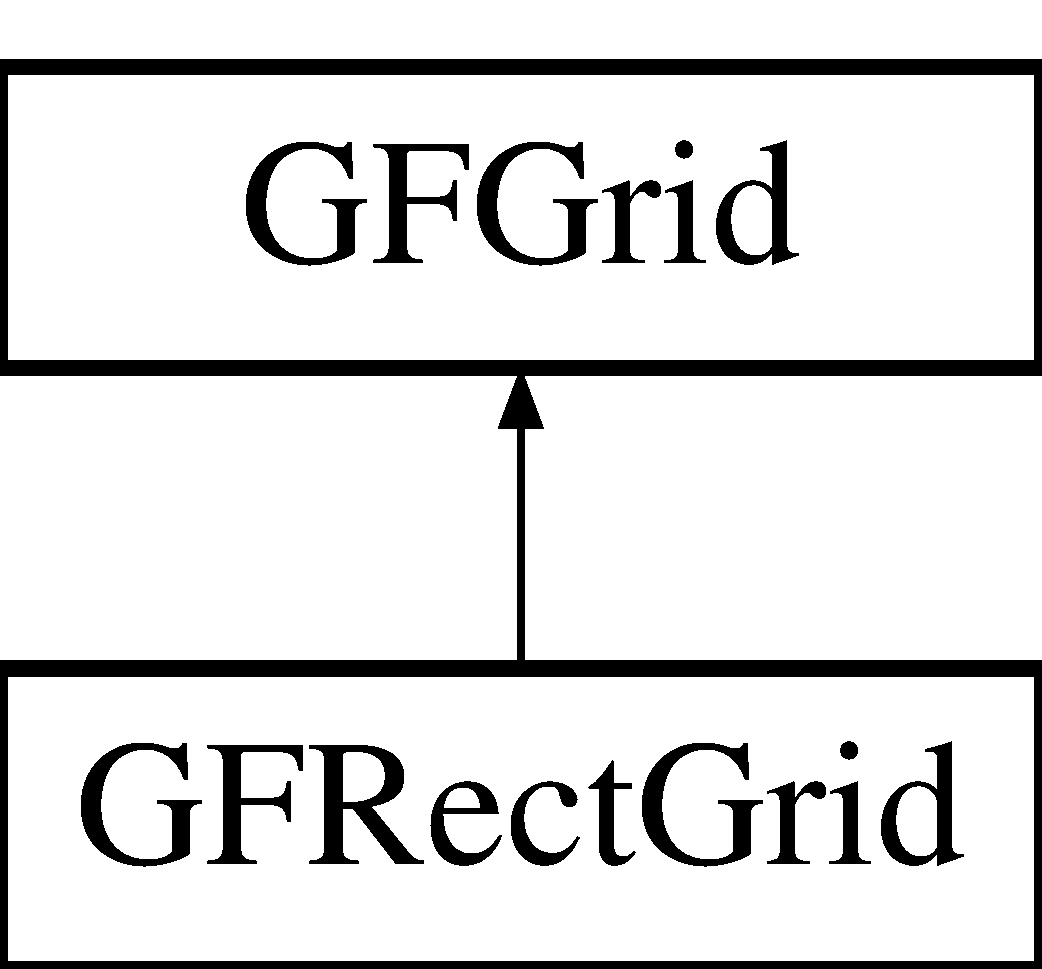
\includegraphics[height=2.000000cm]{class_g_f_rect_grid}
\end{center}
\end{figure}
\subsection*{Public Member Functions}
\begin{DoxyCompactItemize}
\item 
override Vector3 \hyperlink{class_g_f_rect_grid_ac668541585726a76ba85d1e15ca45753_ac668541585726a76ba85d1e15ca45753}{World\+To\+Grid} (Vector3 world\+Point)
\begin{DoxyCompactList}\small\item\em Converts world coordinates to grid coordinates.\end{DoxyCompactList}\item 
override Vector3 \hyperlink{class_g_f_rect_grid_acdc111b97728b0fef0c32e2d96d59f90_acdc111b97728b0fef0c32e2d96d59f90}{Grid\+To\+World} (Vector3 grid\+Point)
\begin{DoxyCompactList}\small\item\em Converts grid coordinates to world coordinates.\end{DoxyCompactList}\item 
override Vector3 \hyperlink{class_g_f_rect_grid_a5c6ed872be90dad1f7868576d513fa05_a5c6ed872be90dad1f7868576d513fa05}{Nearest\+Vertex\+W} (Vector3 world\+Point, bool do\+Debug)
\item 
override Vector3 \hyperlink{class_g_f_rect_grid_a8a81dba8cdb3224a5e3952f903c80d31_a8a81dba8cdb3224a5e3952f903c80d31}{Nearest\+Face\+W} (Vector3 world\+Point, \hyperlink{namespace_grid_framework_aa55de93079e09bd55c4cb660025820d5_aa55de93079e09bd55c4cb660025820d5}{Grid\+Plane} plane, bool do\+Debug)
\begin{DoxyCompactList}\small\item\em Returns the world position of the nearest face.\end{DoxyCompactList}\item 
override Vector3 \hyperlink{class_g_f_rect_grid_a36755945173349f1d24c3a41092bc6f4_a36755945173349f1d24c3a41092bc6f4}{Nearest\+Box\+W} (Vector3 world\+Point, bool do\+Debug)
\begin{DoxyCompactList}\small\item\em Returns the world position of the nearest box.\end{DoxyCompactList}\item 
override Vector3 \hyperlink{class_g_f_rect_grid_a9077b997603860bf0544ceed66325109_a9077b997603860bf0544ceed66325109}{Nearest\+Vertex\+G} (Vector3 world\+Point)
\begin{DoxyCompactList}\small\item\em Returns the grid position of the nearest vertex.\end{DoxyCompactList}\item 
override Vector3 \hyperlink{class_g_f_rect_grid_aeda4f7e218bf92e1cc1361913569fabb_aeda4f7e218bf92e1cc1361913569fabb}{Nearest\+Face\+G} (Vector3 world\+Point, \hyperlink{namespace_grid_framework_aa55de93079e09bd55c4cb660025820d5_aa55de93079e09bd55c4cb660025820d5}{Grid\+Plane} plane)
\begin{DoxyCompactList}\small\item\em Returns the grid position of the nearest face.\end{DoxyCompactList}\item 
override Vector3 \hyperlink{class_g_f_rect_grid_a97bcb6df6296fac0bcf92c9d8908df00_a97bcb6df6296fac0bcf92c9d8908df00}{Nearest\+Box\+G} (Vector3 world\+Point)
\begin{DoxyCompactList}\small\item\em Returns the grid position of the nearest box.\end{DoxyCompactList}\item 
override Vector3 \hyperlink{class_g_f_rect_grid_a26011b42493622436cd9a86516b82687_a26011b42493622436cd9a86516b82687}{Align\+Vector3} (Vector3 pos, Vector3 scale, \hyperlink{class_grid_framework_1_1_vectors_1_1_bool_vector3}{Bool\+Vector3} ignore\+Axis)
\begin{DoxyCompactList}\small\item\em Fits a position vector into the grid.\end{DoxyCompactList}\item 
override Vector3 \hyperlink{class_g_f_rect_grid_a31346980b7fc37aea46e750958c67963_a31346980b7fc37aea46e750958c67963}{Scale\+Vector3} (Vector3 scl, \hyperlink{class_grid_framework_1_1_vectors_1_1_bool_vector3}{Bool\+Vector3} ignore\+Axis)
\begin{DoxyCompactList}\small\item\em Scales a size to fit inside the grid.\end{DoxyCompactList}\end{DoxyCompactItemize}
\subsection*{Properties}
\begin{DoxyCompactItemize}
\item 
Vector3 \hyperlink{class_g_f_rect_grid_a149aa6bd8f08def54ce1b9dd843b6421_a149aa6bd8f08def54ce1b9dd843b6421}{spacing}\hspace{0.3cm}{\ttfamily  \mbox{[}get, set\mbox{]}}
\begin{DoxyCompactList}\small\item\em How large the grid boxes are.\end{DoxyCompactList}\item 
\hyperlink{class_grid_framework_1_1_vectors_1_1_vector6}{Vector6} \hyperlink{class_g_f_rect_grid_af0534ff36d0058a2b00ea898c9ceadf6_af0534ff36d0058a2b00ea898c9ceadf6}{shearing}\hspace{0.3cm}{\ttfamily  \mbox{[}get, set\mbox{]}}
\begin{DoxyCompactList}\small\item\em How the axes are sheared.\end{DoxyCompactList}\item 
Vector3 \hyperlink{class_g_f_rect_grid_acaaffd9ca33010bfb39b1b032b283d81_acaaffd9ca33010bfb39b1b032b283d81}{right}\hspace{0.3cm}{\ttfamily  \mbox{[}get\mbox{]}}
\begin{DoxyCompactList}\small\item\em Direction along the X-\/axis of the grid in world space.\end{DoxyCompactList}\item 
Vector3 \hyperlink{class_g_f_rect_grid_a4e395afadccb994ea1faff1bdf9d7416_a4e395afadccb994ea1faff1bdf9d7416}{up}\hspace{0.3cm}{\ttfamily  \mbox{[}get\mbox{]}}
\begin{DoxyCompactList}\small\item\em Direction along the Y-\/axis of the grid in world space.\end{DoxyCompactList}\item 
Vector3 \hyperlink{class_g_f_rect_grid_a64e371af00fca22f78362473730d4919_a64e371af00fca22f78362473730d4919}{forward}\hspace{0.3cm}{\ttfamily  \mbox{[}get\mbox{]}}
\begin{DoxyCompactList}\small\item\em Direction along the Z-\/axis of the grid in world space.\end{DoxyCompactList}\end{DoxyCompactItemize}
\subsection*{Additional Inherited Members}


\subsection{Detailed Description}
Your standard rectangular grid, the characterising values is its spacing, which can be set for each axis individually. 

\subsection{Member Function Documentation}
\hypertarget{class_g_f_rect_grid_a26011b42493622436cd9a86516b82687_a26011b42493622436cd9a86516b82687}{\index{G\+F\+Rect\+Grid@{G\+F\+Rect\+Grid}!Align\+Vector3@{Align\+Vector3}}
\index{Align\+Vector3@{Align\+Vector3}!G\+F\+Rect\+Grid@{G\+F\+Rect\+Grid}}
\subsubsection[{Align\+Vector3}]{\setlength{\rightskip}{0pt plus 5cm}override Vector3 G\+F\+Rect\+Grid.\+Align\+Vector3 (
\begin{DoxyParamCaption}
\item[{Vector3}]{pos, }
\item[{Vector3}]{scale, }
\item[{{\bf Bool\+Vector3}}]{ignore\+Axis}
\end{DoxyParamCaption}
)\hspace{0.3cm}{\ttfamily [virtual]}}}\label{class_g_f_rect_grid_a26011b42493622436cd9a86516b82687_a26011b42493622436cd9a86516b82687}
\begin{DoxyReturn}{Returns}
Aligned position vector.
\end{DoxyReturn}

\begin{DoxyParams}{Parameters}
{\em pos} & The position to align.\\
\hline
{\em scale} & A simulated scale to decide how exactly to fit the poistion into the grid.\\
\hline
{\em ignore\+Axis} & Which axes should be ignored.\\
\hline
\end{DoxyParams}


This method aligns a point to the grid. The {\itshape scale} parameter is needed to simulate the “size” of point, which influences the resulting position like the scale of a Transform would do above. By default it’s set to one on all axes, placing the point at the centre of a box. If a component of {\ttfamily scale} is odd that component of the vector will be placed between edges, otherwise it will be placed on the nearest edge. The {\ttfamily lock\+Axis} parameter lets you ignore individual axes. 

Implements \hyperlink{class_g_f_grid_a18b3e57431dc0db8f651479e4fb04a8f_a18b3e57431dc0db8f651479e4fb04a8f}{G\+F\+Grid}.

\hypertarget{class_g_f_rect_grid_acdc111b97728b0fef0c32e2d96d59f90_acdc111b97728b0fef0c32e2d96d59f90}{\index{G\+F\+Rect\+Grid@{G\+F\+Rect\+Grid}!Grid\+To\+World@{Grid\+To\+World}}
\index{Grid\+To\+World@{Grid\+To\+World}!G\+F\+Rect\+Grid@{G\+F\+Rect\+Grid}}
\subsubsection[{Grid\+To\+World}]{\setlength{\rightskip}{0pt plus 5cm}override Vector3 G\+F\+Rect\+Grid.\+Grid\+To\+World (
\begin{DoxyParamCaption}
\item[{Vector3}]{grid\+Point}
\end{DoxyParamCaption}
)\hspace{0.3cm}{\ttfamily [virtual]}}}\label{class_g_f_rect_grid_acdc111b97728b0fef0c32e2d96d59f90_acdc111b97728b0fef0c32e2d96d59f90}
\begin{DoxyReturn}{Returns}
World coordinates of the Grid point.
\end{DoxyReturn}

\begin{DoxyParams}{Parameters}
{\em grid\+Point} & Point in grid space.\\
\hline
\end{DoxyParams}


The opposite of \hyperlink{class_g_f_rect_grid_ac668541585726a76ba85d1e15ca45753_ac668541585726a76ba85d1e15ca45753}{World\+To\+Grid}, this returns the world position of a point in the grid. The origin of the grid is the world position of its Game\+Object and its axes lie on the corresponding axes of the Transform. Rotation is taken into account for this operation. 

Implements \hyperlink{class_g_f_grid_af32d7bfcecb5da3fdc47b972b551e33e_af32d7bfcecb5da3fdc47b972b551e33e}{G\+F\+Grid}.

\hypertarget{class_g_f_rect_grid_a97bcb6df6296fac0bcf92c9d8908df00_a97bcb6df6296fac0bcf92c9d8908df00}{\index{G\+F\+Rect\+Grid@{G\+F\+Rect\+Grid}!Nearest\+Box\+G@{Nearest\+Box\+G}}
\index{Nearest\+Box\+G@{Nearest\+Box\+G}!G\+F\+Rect\+Grid@{G\+F\+Rect\+Grid}}
\subsubsection[{Nearest\+Box\+G}]{\setlength{\rightskip}{0pt plus 5cm}override Vector3 G\+F\+Rect\+Grid.\+Nearest\+Box\+G (
\begin{DoxyParamCaption}
\item[{Vector3}]{world\+Point}
\end{DoxyParamCaption}
)\hspace{0.3cm}{\ttfamily [virtual]}}}\label{class_g_f_rect_grid_a97bcb6df6296fac0bcf92c9d8908df00_a97bcb6df6296fac0bcf92c9d8908df00}
\begin{DoxyReturn}{Returns}
Grid position of the nearest box.
\end{DoxyReturn}

\begin{DoxyParams}{Parameters}
{\em world\+Point} & Point in world space.\\
\hline
\end{DoxyParams}


Similar to {\ttfamily \hyperlink{class_g_f_rect_grid_a36755945173349f1d24c3a41092bc6f4_a36755945173349f1d24c3a41092bc6f4}{Nearest\+Box\+W}}, except you get grid coordinates instead of world coordinates. Since faces lie between vertices all three values will always have +0.5 compared to vertex coordinates.  Example\+: {\ttfamily  \hyperlink{class_g_f_rect_grid}{G\+F\+Rect\+Grid} my\+Grid; Vector3 world\+Point; Vector3 box = my\+Grid.\+Nearest\+Box\+G(world\+Point); // something like (2.\+5, -\/1.\+5, 3.\+5) } 

Implements \hyperlink{class_g_f_grid_adb7c70449b2449c1e82132e6300cc1a5_adb7c70449b2449c1e82132e6300cc1a5}{G\+F\+Grid}.

\hypertarget{class_g_f_rect_grid_a36755945173349f1d24c3a41092bc6f4_a36755945173349f1d24c3a41092bc6f4}{\index{G\+F\+Rect\+Grid@{G\+F\+Rect\+Grid}!Nearest\+Box\+W@{Nearest\+Box\+W}}
\index{Nearest\+Box\+W@{Nearest\+Box\+W}!G\+F\+Rect\+Grid@{G\+F\+Rect\+Grid}}
\subsubsection[{Nearest\+Box\+W}]{\setlength{\rightskip}{0pt plus 5cm}override Vector3 G\+F\+Rect\+Grid.\+Nearest\+Box\+W (
\begin{DoxyParamCaption}
\item[{Vector3}]{world\+Point, }
\item[{bool}]{do\+Debug}
\end{DoxyParamCaption}
)\hspace{0.3cm}{\ttfamily [virtual]}}}\label{class_g_f_rect_grid_a36755945173349f1d24c3a41092bc6f4_a36755945173349f1d24c3a41092bc6f4}
\begin{DoxyReturn}{Returns}
World position of the nearest box.
\end{DoxyReturn}

\begin{DoxyParams}{Parameters}
{\em world\+Point} & Point in world space.\\
\hline
{\em do\+Debug} & Whether to draw a small debug sphere at the box.\\
\hline
\end{DoxyParams}


Similar to \hyperlink{class_g_f_rect_grid_a5c6ed872be90dad1f7868576d513fa05_a5c6ed872be90dad1f7868576d513fa05}{Nearest\+Vertex\+W}, it returns the world coordinates of a box in the grid. Since the box is enclosed by eight vertices, the returned value is the point in between all eight of them. If {\ttfamily do\+Debug} is set a small gizmo box will drawn inside the box. 

Implements \hyperlink{class_g_f_grid_a02fcf02269ca5a2064acccecde9819eb_a02fcf02269ca5a2064acccecde9819eb}{G\+F\+Grid}.

\hypertarget{class_g_f_rect_grid_aeda4f7e218bf92e1cc1361913569fabb_aeda4f7e218bf92e1cc1361913569fabb}{\index{G\+F\+Rect\+Grid@{G\+F\+Rect\+Grid}!Nearest\+Face\+G@{Nearest\+Face\+G}}
\index{Nearest\+Face\+G@{Nearest\+Face\+G}!G\+F\+Rect\+Grid@{G\+F\+Rect\+Grid}}
\subsubsection[{Nearest\+Face\+G}]{\setlength{\rightskip}{0pt plus 5cm}override Vector3 G\+F\+Rect\+Grid.\+Nearest\+Face\+G (
\begin{DoxyParamCaption}
\item[{Vector3}]{world\+Point, }
\item[{{\bf Grid\+Plane}}]{plane}
\end{DoxyParamCaption}
)\hspace{0.3cm}{\ttfamily [virtual]}}}\label{class_g_f_rect_grid_aeda4f7e218bf92e1cc1361913569fabb_aeda4f7e218bf92e1cc1361913569fabb}
\begin{DoxyReturn}{Returns}
Grid position of the nearest face.
\end{DoxyReturn}

\begin{DoxyParams}{Parameters}
{\em world\+Point} & Point in world space.\\
\hline
{\em plane} & Plane on which the face lies.\\
\hline
\end{DoxyParams}


Similar to \hyperlink{class_g_f_rect_grid_a8a81dba8cdb3224a5e3952f903c80d31_a8a81dba8cdb3224a5e3952f903c80d31}{Nearest\+Face\+W}, except you get grid coordinates instead of world coordinates. Since faces lie between vertices two values will always have +0.5 compared to vertex coordinates, while the values that lies on the plane will have a round number.  Example\+: {\ttfamily  \hyperlink{class_g_f_rect_grid}{G\+F\+Rect\+Grid} my\+Grid; Vector3 world\+Point; Vector3 face = my\+Grid.\+Nearest\+Face\+G(world\+Point, G\+F\+Grid.\+Grid\+Plane.\+X\+Y); // something like (2.\+5, -\/1.\+5, 3) } 

Implements \hyperlink{class_g_f_grid_aac129f3df1da5cdbc31143ecc7db35d2_aac129f3df1da5cdbc31143ecc7db35d2}{G\+F\+Grid}.

\hypertarget{class_g_f_rect_grid_a8a81dba8cdb3224a5e3952f903c80d31_a8a81dba8cdb3224a5e3952f903c80d31}{\index{G\+F\+Rect\+Grid@{G\+F\+Rect\+Grid}!Nearest\+Face\+W@{Nearest\+Face\+W}}
\index{Nearest\+Face\+W@{Nearest\+Face\+W}!G\+F\+Rect\+Grid@{G\+F\+Rect\+Grid}}
\subsubsection[{Nearest\+Face\+W}]{\setlength{\rightskip}{0pt plus 5cm}override Vector3 G\+F\+Rect\+Grid.\+Nearest\+Face\+W (
\begin{DoxyParamCaption}
\item[{Vector3}]{world\+Point, }
\item[{{\bf Grid\+Plane}}]{plane, }
\item[{bool}]{do\+Debug}
\end{DoxyParamCaption}
)\hspace{0.3cm}{\ttfamily [virtual]}}}\label{class_g_f_rect_grid_a8a81dba8cdb3224a5e3952f903c80d31_a8a81dba8cdb3224a5e3952f903c80d31}
\begin{DoxyReturn}{Returns}
World position of the nearest face.
\end{DoxyReturn}

\begin{DoxyParams}{Parameters}
{\em world\+Point} & Point in world space.\\
\hline
{\em plane} & Plane on which the face lies.\\
\hline
{\em do\+Debug} & Whether to draw a small debug sphere at the vertex.\\
\hline
\end{DoxyParams}


Similar to \hyperlink{class_g_f_rect_grid_a5c6ed872be90dad1f7868576d513fa05_a5c6ed872be90dad1f7868576d513fa05}{Nearest\+Vertex\+W}, it returns the world coordinates of a face on the grid. Since the face is enclosed by four vertices, the returned value is the point in between all four of the vertices. You also need to specify on which plane the face lies. If {\ttfamily do\+Debug} is set a small gizmo face will drawn inside the face. 

Implements \hyperlink{class_g_f_grid_ae8711b08c90871f6e88800a30ff5077f_ae8711b08c90871f6e88800a30ff5077f}{G\+F\+Grid}.

\hypertarget{class_g_f_rect_grid_a9077b997603860bf0544ceed66325109_a9077b997603860bf0544ceed66325109}{\index{G\+F\+Rect\+Grid@{G\+F\+Rect\+Grid}!Nearest\+Vertex\+G@{Nearest\+Vertex\+G}}
\index{Nearest\+Vertex\+G@{Nearest\+Vertex\+G}!G\+F\+Rect\+Grid@{G\+F\+Rect\+Grid}}
\subsubsection[{Nearest\+Vertex\+G}]{\setlength{\rightskip}{0pt plus 5cm}override Vector3 G\+F\+Rect\+Grid.\+Nearest\+Vertex\+G (
\begin{DoxyParamCaption}
\item[{Vector3}]{world\+Point}
\end{DoxyParamCaption}
)\hspace{0.3cm}{\ttfamily [virtual]}}}\label{class_g_f_rect_grid_a9077b997603860bf0544ceed66325109_a9077b997603860bf0544ceed66325109}
\begin{DoxyReturn}{Returns}
Grid position of the nearest vertex.
\end{DoxyReturn}

\begin{DoxyParams}{Parameters}
{\em world\+Point} & Point in world space.\\
\hline
\end{DoxyParams}


Similar to {\ttfamily \hyperlink{class_g_f_rect_grid_a5c6ed872be90dad1f7868576d513fa05_a5c6ed872be90dad1f7868576d513fa05}{Nearest\+Vertex\+W}}, except you get grid coordinates instead of world coordinates. 

Implements \hyperlink{class_g_f_grid_a7eaa2821cf118bb4821bd2cbf40029da_a7eaa2821cf118bb4821bd2cbf40029da}{G\+F\+Grid}.

\hypertarget{class_g_f_rect_grid_a5c6ed872be90dad1f7868576d513fa05_a5c6ed872be90dad1f7868576d513fa05}{\index{G\+F\+Rect\+Grid@{G\+F\+Rect\+Grid}!Nearest\+Vertex\+W@{Nearest\+Vertex\+W}}
\index{Nearest\+Vertex\+W@{Nearest\+Vertex\+W}!G\+F\+Rect\+Grid@{G\+F\+Rect\+Grid}}
\subsubsection[{Nearest\+Vertex\+W}]{\setlength{\rightskip}{0pt plus 5cm}override Vector3 G\+F\+Rect\+Grid.\+Nearest\+Vertex\+W (
\begin{DoxyParamCaption}
\item[{Vector3}]{world\+Point, }
\item[{bool}]{do\+Debug}
\end{DoxyParamCaption}
)\hspace{0.3cm}{\ttfamily [virtual]}}}\label{class_g_f_rect_grid_a5c6ed872be90dad1f7868576d513fa05_a5c6ed872be90dad1f7868576d513fa05}
Returns the world position of the nearest vertex from a given point in world space. If {\ttfamily do\+Debug} is set a small gizmo sphere will be drawn at the vertex position. 

Implements \hyperlink{class_g_f_grid_a5865880fa767bf5562301bca419b8bb9_a5865880fa767bf5562301bca419b8bb9}{G\+F\+Grid}.

\hypertarget{class_g_f_rect_grid_a31346980b7fc37aea46e750958c67963_a31346980b7fc37aea46e750958c67963}{\index{G\+F\+Rect\+Grid@{G\+F\+Rect\+Grid}!Scale\+Vector3@{Scale\+Vector3}}
\index{Scale\+Vector3@{Scale\+Vector3}!G\+F\+Rect\+Grid@{G\+F\+Rect\+Grid}}
\subsubsection[{Scale\+Vector3}]{\setlength{\rightskip}{0pt plus 5cm}override Vector3 G\+F\+Rect\+Grid.\+Scale\+Vector3 (
\begin{DoxyParamCaption}
\item[{Vector3}]{scl, }
\item[{{\bf Bool\+Vector3}}]{ignore\+Axis}
\end{DoxyParamCaption}
)\hspace{0.3cm}{\ttfamily [virtual]}}}\label{class_g_f_rect_grid_a31346980b7fc37aea46e750958c67963_a31346980b7fc37aea46e750958c67963}
\begin{DoxyReturn}{Returns}
The re-\/scaled vector.
\end{DoxyReturn}

\begin{DoxyParams}{Parameters}
{\em scl} & The vector to scale.\\
\hline
{\em ignore\+Axis} & The axes to ignore.\\
\hline
\end{DoxyParams}


Scales a size to the nearest multiple of the grid’s spacing. The parameter {\itshape ignore\+Axis} makes the function not touch the corresponding coordinate. 

Implements \hyperlink{class_g_f_grid_a02b3cf14a1529355c51e0d3ea646b4f8_a02b3cf14a1529355c51e0d3ea646b4f8}{G\+F\+Grid}.

\hypertarget{class_g_f_rect_grid_ac668541585726a76ba85d1e15ca45753_ac668541585726a76ba85d1e15ca45753}{\index{G\+F\+Rect\+Grid@{G\+F\+Rect\+Grid}!World\+To\+Grid@{World\+To\+Grid}}
\index{World\+To\+Grid@{World\+To\+Grid}!G\+F\+Rect\+Grid@{G\+F\+Rect\+Grid}}
\subsubsection[{World\+To\+Grid}]{\setlength{\rightskip}{0pt plus 5cm}override Vector3 G\+F\+Rect\+Grid.\+World\+To\+Grid (
\begin{DoxyParamCaption}
\item[{Vector3}]{world\+Point}
\end{DoxyParamCaption}
)\hspace{0.3cm}{\ttfamily [virtual]}}}\label{class_g_f_rect_grid_ac668541585726a76ba85d1e15ca45753_ac668541585726a76ba85d1e15ca45753}
\begin{DoxyReturn}{Returns}
Grid coordinates of the world point.
\end{DoxyReturn}

\begin{DoxyParams}{Parameters}
{\em world\+Point} & Point in world space.\\
\hline
\end{DoxyParams}


Takes in a position in wold space and calculates where in the grid that position is. The origin of the grid is the world position of its Game\+Object and its axes lie on the corresponding axes of the Transform. Rotation is taken into account for this operation. 

Implements \hyperlink{class_g_f_grid_a3c424ac71404a8c87a958b5b5952eb0f_a3c424ac71404a8c87a958b5b5952eb0f}{G\+F\+Grid}.



\subsection{Property Documentation}
\hypertarget{class_g_f_rect_grid_a64e371af00fca22f78362473730d4919_a64e371af00fca22f78362473730d4919}{\index{G\+F\+Rect\+Grid@{G\+F\+Rect\+Grid}!forward@{forward}}
\index{forward@{forward}!G\+F\+Rect\+Grid@{G\+F\+Rect\+Grid}}
\subsubsection[{forward}]{\setlength{\rightskip}{0pt plus 5cm}Vector3 G\+F\+Rect\+Grid.\+forward\hspace{0.3cm}{\ttfamily [get]}}}\label{class_g_f_rect_grid_a64e371af00fca22f78362473730d4919_a64e371af00fca22f78362473730d4919}
Unit vector in grid scale along the grid's Z-\/axis.

The Z-\/axis of the grid in world space. This is a shorthand writing for {\ttfamily spacing.\+z $\ast$ transform.\+forward}. The value is read-\/only. \hypertarget{class_g_f_rect_grid_acaaffd9ca33010bfb39b1b032b283d81_acaaffd9ca33010bfb39b1b032b283d81}{\index{G\+F\+Rect\+Grid@{G\+F\+Rect\+Grid}!right@{right}}
\index{right@{right}!G\+F\+Rect\+Grid@{G\+F\+Rect\+Grid}}
\subsubsection[{right}]{\setlength{\rightskip}{0pt plus 5cm}Vector3 G\+F\+Rect\+Grid.\+right\hspace{0.3cm}{\ttfamily [get]}}}\label{class_g_f_rect_grid_acaaffd9ca33010bfb39b1b032b283d81_acaaffd9ca33010bfb39b1b032b283d81}
Unit vector in grid scale along the grid's X-\/axis.

The X-\/axis of the grid in world space. This is a shorthand writing for {\ttfamily spacing.\+x $\ast$ transform.\+right}. The value is read-\/only. \hypertarget{class_g_f_rect_grid_af0534ff36d0058a2b00ea898c9ceadf6_af0534ff36d0058a2b00ea898c9ceadf6}{\index{G\+F\+Rect\+Grid@{G\+F\+Rect\+Grid}!shearing@{shearing}}
\index{shearing@{shearing}!G\+F\+Rect\+Grid@{G\+F\+Rect\+Grid}}
\subsubsection[{shearing}]{\setlength{\rightskip}{0pt plus 5cm}{\bf Vector6} G\+F\+Rect\+Grid.\+shearing\hspace{0.3cm}{\ttfamily [get]}, {\ttfamily [set]}}}\label{class_g_f_rect_grid_af0534ff36d0058a2b00ea898c9ceadf6_af0534ff36d0058a2b00ea898c9ceadf6}
Shearing vector of the grid.

How much the individual axes of the grid are skewed towards each other. For instance, this means the if {\itshape X\+Y} is set to {\itshape 2}, then for each point with grid coordinates \+\_\+(x, y)\+\_\+ will be mapped to \+\_\+(x, y + 2x)\+\_\+, while the uninvolved {\itshape Z} coordinate remains the same. For more information refer to the manual. \hypertarget{class_g_f_rect_grid_a149aa6bd8f08def54ce1b9dd843b6421_a149aa6bd8f08def54ce1b9dd843b6421}{\index{G\+F\+Rect\+Grid@{G\+F\+Rect\+Grid}!spacing@{spacing}}
\index{spacing@{spacing}!G\+F\+Rect\+Grid@{G\+F\+Rect\+Grid}}
\subsubsection[{spacing}]{\setlength{\rightskip}{0pt plus 5cm}Vector3 G\+F\+Rect\+Grid.\+spacing\hspace{0.3cm}{\ttfamily [get]}, {\ttfamily [set]}}}\label{class_g_f_rect_grid_a149aa6bd8f08def54ce1b9dd843b6421_a149aa6bd8f08def54ce1b9dd843b6421}
The spacing of the grid.

How far apart the lines of the grid are. You can set each axis separately, but none may be less than 0.\+1, in order to prevent values that don't make any sense. \hypertarget{class_g_f_rect_grid_a4e395afadccb994ea1faff1bdf9d7416_a4e395afadccb994ea1faff1bdf9d7416}{\index{G\+F\+Rect\+Grid@{G\+F\+Rect\+Grid}!up@{up}}
\index{up@{up}!G\+F\+Rect\+Grid@{G\+F\+Rect\+Grid}}
\subsubsection[{up}]{\setlength{\rightskip}{0pt plus 5cm}Vector3 G\+F\+Rect\+Grid.\+up\hspace{0.3cm}{\ttfamily [get]}}}\label{class_g_f_rect_grid_a4e395afadccb994ea1faff1bdf9d7416_a4e395afadccb994ea1faff1bdf9d7416}
Unit vector in grid scale along the grid's Y-\/axis.

The Y-\/axis of the grid in world space. This is a shorthand writing for {\ttfamily spacing.\+y $\ast$ transform.\+up}. The value is read-\/only. 

The documentation for this class was generated from the following file\+:\begin{DoxyCompactItemize}
\item 
G\+F\+Rect\+Grid.\+cs\end{DoxyCompactItemize}

\hypertarget{class_grid_framework_1_1_vectors_1_1_vector6}{\section{Grid\+Framework.\+Vectors.\+Vector6 Class Reference}
\label{class_grid_framework_1_1_vectors_1_1_vector6}\index{Grid\+Framework.\+Vectors.\+Vector6@{Grid\+Framework.\+Vectors.\+Vector6}}
}


Class representing six adjacent float values for the shearing of a rectangular grid. 




Inherits I\+Equatable$<$ Vector6 $>$.

\subsection*{Public Member Functions}
\begin{DoxyCompactItemize}
\item 
\hyperlink{class_grid_framework_1_1_vectors_1_1_vector6_ab23b9c6788f639892c0d258f7ce9a3d8_ab23b9c6788f639892c0d258f7ce9a3d8}{Vector6} (float \hyperlink{class_grid_framework_1_1_vectors_1_1_vector6_a2ad5ebb8120ce653ef9201f60fa266b2_a2ad5ebb8120ce653ef9201f60fa266b2}{xy}, float \hyperlink{class_grid_framework_1_1_vectors_1_1_vector6_a3e756c556026961df6d0e0ae5172df16_a3e756c556026961df6d0e0ae5172df16}{xz}, float \hyperlink{class_grid_framework_1_1_vectors_1_1_vector6_a6a73271b83f35cdf32b17131eb4e2900_a6a73271b83f35cdf32b17131eb4e2900}{yx}, float \hyperlink{class_grid_framework_1_1_vectors_1_1_vector6_a4f22ae6f20adcd03c347f40c7f92ec1f_a4f22ae6f20adcd03c347f40c7f92ec1f}{yz}, float \hyperlink{class_grid_framework_1_1_vectors_1_1_vector6_ab27c48ff072b75aaf98fff8ef0a49824_ab27c48ff072b75aaf98fff8ef0a49824}{zx}, float \hyperlink{class_grid_framework_1_1_vectors_1_1_vector6_a5e2ba27db4f2995d97dba42905370e50_a5e2ba27db4f2995d97dba42905370e50}{zy})
\begin{DoxyCompactList}\small\item\em Creates a new vector with given values.\end{DoxyCompactList}\item 
\hyperlink{class_grid_framework_1_1_vectors_1_1_vector6_a6f72df5771b3696df8720da733c89397_a6f72df5771b3696df8720da733c89397}{Vector6} (float value)
\begin{DoxyCompactList}\small\item\em Creates a new vector with all values set to the same value.\end{DoxyCompactList}\item 
\hyperlink{class_grid_framework_1_1_vectors_1_1_vector6_a19e941a52546077675a2500b5e570b77_a19e941a52546077675a2500b5e570b77}{Vector6} (\hyperlink{class_grid_framework_1_1_vectors_1_1_vector6}{Vector6} original)
\begin{DoxyCompactList}\small\item\em Creates a new vector from an existing vector.\end{DoxyCompactList}\item 
\hyperlink{class_grid_framework_1_1_vectors_1_1_vector6_a6f5f6e1a150eaf2e2db49f368773b99c_a6f5f6e1a150eaf2e2db49f368773b99c}{Vector6} ()
\begin{DoxyCompactList}\small\item\em Creates a new vector with undefined, but allocated values.\end{DoxyCompactList}\item 
void \hyperlink{class_grid_framework_1_1_vectors_1_1_vector6_a5f5e7129e8362d153d5e6a4068b532c5_a5f5e7129e8362d153d5e6a4068b532c5}{Set} (float \hyperlink{class_grid_framework_1_1_vectors_1_1_vector6_a2ad5ebb8120ce653ef9201f60fa266b2_a2ad5ebb8120ce653ef9201f60fa266b2}{xy}, float \hyperlink{class_grid_framework_1_1_vectors_1_1_vector6_a3e756c556026961df6d0e0ae5172df16_a3e756c556026961df6d0e0ae5172df16}{xz}, float \hyperlink{class_grid_framework_1_1_vectors_1_1_vector6_a6a73271b83f35cdf32b17131eb4e2900_a6a73271b83f35cdf32b17131eb4e2900}{yx}, float \hyperlink{class_grid_framework_1_1_vectors_1_1_vector6_a4f22ae6f20adcd03c347f40c7f92ec1f_a4f22ae6f20adcd03c347f40c7f92ec1f}{yz}, float \hyperlink{class_grid_framework_1_1_vectors_1_1_vector6_ab27c48ff072b75aaf98fff8ef0a49824_ab27c48ff072b75aaf98fff8ef0a49824}{zx}, float \hyperlink{class_grid_framework_1_1_vectors_1_1_vector6_a5e2ba27db4f2995d97dba42905370e50_a5e2ba27db4f2995d97dba42905370e50}{zy})
\begin{DoxyCompactList}\small\item\em Set the values of the vector manually.\end{DoxyCompactList}\item 
void \hyperlink{class_grid_framework_1_1_vectors_1_1_vector6_ab237e85472bf99b09ed2ab1ba4e39991_ab237e85472bf99b09ed2ab1ba4e39991}{Set} (float value, int index)
\begin{DoxyCompactList}\small\item\em Set a value of the vector at a certain index.\end{DoxyCompactList}\item 
void \hyperlink{class_grid_framework_1_1_vectors_1_1_vector6_a181965c9505b6136a366744d28e1d0f9_a181965c9505b6136a366744d28e1d0f9}{Set} (float value, \hyperlink{namespace_grid_framework_1_1_vectors_ad130792047c0f851300f88c95d1b8280_ad130792047c0f851300f88c95d1b8280}{Axis2} component)
\begin{DoxyCompactList}\small\item\em Set a value of the vector at a certain component.\end{DoxyCompactList}\item 
void \hyperlink{class_grid_framework_1_1_vectors_1_1_vector6_ab38034d791230d456c188a556001e7f5_ab38034d791230d456c188a556001e7f5}{Set} (Vector2 values, int index)
\begin{DoxyCompactList}\small\item\em Set two values of the vector at a certain index.\end{DoxyCompactList}\item 
void \hyperlink{class_grid_framework_1_1_vectors_1_1_vector6_a12977d2e2d209c261711760c391195c8_a12977d2e2d209c261711760c391195c8}{Set} (Vector2 values, \hyperlink{namespace_grid_framework_1_1_vectors_ad4ae859bed7702114a43e9e1b1b99360_ad4ae859bed7702114a43e9e1b1b99360}{Axis} axis)
\begin{DoxyCompactList}\small\item\em Set two values of the vector at a certain axis.\end{DoxyCompactList}\item 
void \hyperlink{class_grid_framework_1_1_vectors_1_1_vector6_ad689ca1d68c0bf615aca29ded8dc794f_ad689ca1d68c0bf615aca29ded8dc794f}{Set} (\hyperlink{class_grid_framework_1_1_vectors_1_1_vector6}{Vector6} original)
\begin{DoxyCompactList}\small\item\em Copies the values of another vector.\end{DoxyCompactList}\item 
void \hyperlink{class_grid_framework_1_1_vectors_1_1_vector6_ad1c70516cb8ebd4bb3e7027e586fe9f9_ad1c70516cb8ebd4bb3e7027e586fe9f9}{Add} (\hyperlink{class_grid_framework_1_1_vectors_1_1_vector6}{Vector6} summand)
\begin{DoxyCompactList}\small\item\em Adds a vector to this vector.\end{DoxyCompactList}\item 
void \hyperlink{class_grid_framework_1_1_vectors_1_1_vector6_aff32cc229042cc6463e9332dd69f518a_aff32cc229042cc6463e9332dd69f518a}{Subtract} (\hyperlink{class_grid_framework_1_1_vectors_1_1_vector6}{Vector6} subtrahend)
\begin{DoxyCompactList}\small\item\em Subtracts a vector from this vector.\end{DoxyCompactList}\item 
void \hyperlink{class_grid_framework_1_1_vectors_1_1_vector6_ac4e8068cbeb4f8d87bca1ef2abd9f830_ac4e8068cbeb4f8d87bca1ef2abd9f830}{Negate} ()
\begin{DoxyCompactList}\small\item\em Negates a vector.\end{DoxyCompactList}\item 
void \hyperlink{class_grid_framework_1_1_vectors_1_1_vector6_a24874f448a40d22a72469defc2717ca0_a24874f448a40d22a72469defc2717ca0}{Scale} (\hyperlink{class_grid_framework_1_1_vectors_1_1_vector6}{Vector6} factor)
\begin{DoxyCompactList}\small\item\em Scales this vector component-\/wise with another vector.\end{DoxyCompactList}\item 
void \hyperlink{class_grid_framework_1_1_vectors_1_1_vector6_a7ec5913250e83dbc213856475df38970_a7ec5913250e83dbc213856475df38970}{Scale} (float factor)
\begin{DoxyCompactList}\small\item\em Scales this vector component-\/wise with a scalar factor.\end{DoxyCompactList}\item 
void \hyperlink{class_grid_framework_1_1_vectors_1_1_vector6_a4db5e65c63eee368eb69b61e7135f356_a4db5e65c63eee368eb69b61e7135f356}{Max} (\hyperlink{class_grid_framework_1_1_vectors_1_1_vector6}{Vector6} compared\+To)
\begin{DoxyCompactList}\small\item\em Component-\/wise maximum of this vector and another one.\end{DoxyCompactList}\item 
void \hyperlink{class_grid_framework_1_1_vectors_1_1_vector6_a8356582db024654c8694fd46cbfa86b3_a8356582db024654c8694fd46cbfa86b3}{Min} (\hyperlink{class_grid_framework_1_1_vectors_1_1_vector6}{Vector6} compared\+To)
\begin{DoxyCompactList}\small\item\em Component-\/wise minimum of this vector and another one.\end{DoxyCompactList}\item 
void \hyperlink{class_grid_framework_1_1_vectors_1_1_vector6_aae1062c3a23d64c883bd7890e67b9b48_aae1062c3a23d64c883bd7890e67b9b48}{Lerp} (\hyperlink{class_grid_framework_1_1_vectors_1_1_vector6}{Vector6} towards, float t)
\begin{DoxyCompactList}\small\item\em Linearly interpolates a vector with another one.\end{DoxyCompactList}\end{DoxyCompactItemize}
\subsection*{Static Public Member Functions}
\begin{DoxyCompactItemize}
\item 
static \hyperlink{class_grid_framework_1_1_vectors_1_1_vector6}{Vector6} \hyperlink{class_grid_framework_1_1_vectors_1_1_vector6_aead346fb7cdcb61ac670495fe547db35_aead346fb7cdcb61ac670495fe547db35}{Add} (\hyperlink{class_grid_framework_1_1_vectors_1_1_vector6}{Vector6} summand1, \hyperlink{class_grid_framework_1_1_vectors_1_1_vector6}{Vector6} summand2)
\begin{DoxyCompactList}\small\item\em Adds two vectors and returns the result as a new vector.\end{DoxyCompactList}\item 
static \hyperlink{class_grid_framework_1_1_vectors_1_1_vector6}{Vector6} \hyperlink{class_grid_framework_1_1_vectors_1_1_vector6_afdccc269b1d2cc05b601f13bec6cf6c3_afdccc269b1d2cc05b601f13bec6cf6c3}{Subtract} (\hyperlink{class_grid_framework_1_1_vectors_1_1_vector6}{Vector6} minuend, \hyperlink{class_grid_framework_1_1_vectors_1_1_vector6}{Vector6} subtrahend)
\begin{DoxyCompactList}\small\item\em Subtracts two vectors and returns the result as a new vector.\end{DoxyCompactList}\item 
static \hyperlink{class_grid_framework_1_1_vectors_1_1_vector6}{Vector6} \hyperlink{class_grid_framework_1_1_vectors_1_1_vector6_a9c64543e1963092f36376d07105a69cc_a9c64543e1963092f36376d07105a69cc}{Negate} (\hyperlink{class_grid_framework_1_1_vectors_1_1_vector6}{Vector6} value)
\begin{DoxyCompactList}\small\item\em Negates a vector and returns the result as a new vector.\end{DoxyCompactList}\item 
static \hyperlink{class_grid_framework_1_1_vectors_1_1_vector6}{Vector6} \hyperlink{class_grid_framework_1_1_vectors_1_1_vector6_aed5217185ac89f4ce93477ec9b5c752b_aed5217185ac89f4ce93477ec9b5c752b}{Scale} (\hyperlink{class_grid_framework_1_1_vectors_1_1_vector6}{Vector6} factor1, \hyperlink{class_grid_framework_1_1_vectors_1_1_vector6}{Vector6} factor2)
\begin{DoxyCompactList}\small\item\em Scales a vector component-\/wise with another vector and returns the result as a new vector.\end{DoxyCompactList}\item 
static \hyperlink{class_grid_framework_1_1_vectors_1_1_vector6}{Vector6} \hyperlink{class_grid_framework_1_1_vectors_1_1_vector6_af1b84072dea3102258eb7bd22a9e5d7c_af1b84072dea3102258eb7bd22a9e5d7c}{Scale} (\hyperlink{class_grid_framework_1_1_vectors_1_1_vector6}{Vector6} vector, float factor)
\begin{DoxyCompactList}\small\item\em Scales a vector component-\/wise with a scalar factor and returns the result as a new vector.\end{DoxyCompactList}\item 
static \hyperlink{class_grid_framework_1_1_vectors_1_1_vector6}{Vector6} \hyperlink{class_grid_framework_1_1_vectors_1_1_vector6_a6d79343eb75e1a4360dc320591908f13_a6d79343eb75e1a4360dc320591908f13}{Max} (\hyperlink{class_grid_framework_1_1_vectors_1_1_vector6}{Vector6} lhs, \hyperlink{class_grid_framework_1_1_vectors_1_1_vector6}{Vector6} rhs)
\begin{DoxyCompactList}\small\item\em Creates a new vector as the component-\/wise maximum of two vectors.\end{DoxyCompactList}\item 
static \hyperlink{class_grid_framework_1_1_vectors_1_1_vector6}{Vector6} \hyperlink{class_grid_framework_1_1_vectors_1_1_vector6_a849b7f01651b72bbaf876369303351c1_a849b7f01651b72bbaf876369303351c1}{Min} (\hyperlink{class_grid_framework_1_1_vectors_1_1_vector6}{Vector6} lhs, \hyperlink{class_grid_framework_1_1_vectors_1_1_vector6}{Vector6} rhs)
\begin{DoxyCompactList}\small\item\em Creates a new vector as the component-\/wise minimum of two vectors.\end{DoxyCompactList}\item 
static \hyperlink{class_grid_framework_1_1_vectors_1_1_vector6}{Vector6} \hyperlink{class_grid_framework_1_1_vectors_1_1_vector6_aa199e0b3ec5a239f4bbf11f49f082515_aa199e0b3ec5a239f4bbf11f49f082515}{Lerp} (\hyperlink{class_grid_framework_1_1_vectors_1_1_vector6}{Vector6} from, \hyperlink{class_grid_framework_1_1_vectors_1_1_vector6}{Vector6} to, float t)
\begin{DoxyCompactList}\small\item\em Linearly interpolates two vectors and returns the result as a new vector.\end{DoxyCompactList}\item 
static \hyperlink{class_grid_framework_1_1_vectors_1_1_vector6}{Vector6} \hyperlink{class_grid_framework_1_1_vectors_1_1_vector6_ac997ff251a71b75e69048b6e05aba8ec_ac997ff251a71b75e69048b6e05aba8ec}{operator+} (\hyperlink{class_grid_framework_1_1_vectors_1_1_vector6}{Vector6} lhs, \hyperlink{class_grid_framework_1_1_vectors_1_1_vector6}{Vector6} rhs)
\begin{DoxyCompactList}\small\item\em Creates a new vector as the sum of two vectors.\end{DoxyCompactList}\item 
static \hyperlink{class_grid_framework_1_1_vectors_1_1_vector6}{Vector6} \hyperlink{class_grid_framework_1_1_vectors_1_1_vector6_adea3b70326107a08d8e27f5ebe287efe_adea3b70326107a08d8e27f5ebe287efe}{operator-\/} (\hyperlink{class_grid_framework_1_1_vectors_1_1_vector6}{Vector6} lhs, \hyperlink{class_grid_framework_1_1_vectors_1_1_vector6}{Vector6} rhs)
\begin{DoxyCompactList}\small\item\em Creates a new vector as the difference of two vectors.\end{DoxyCompactList}\item 
static \hyperlink{class_grid_framework_1_1_vectors_1_1_vector6}{Vector6} \hyperlink{class_grid_framework_1_1_vectors_1_1_vector6_a2ff7010c55e18371374e038d2abdbdd0_a2ff7010c55e18371374e038d2abdbdd0}{operator-\/} (\hyperlink{class_grid_framework_1_1_vectors_1_1_vector6}{Vector6} value)
\begin{DoxyCompactList}\small\item\em Creates a new vector as the negationn of a vector.\end{DoxyCompactList}\item 
static \hyperlink{class_grid_framework_1_1_vectors_1_1_vector6}{Vector6} \hyperlink{class_grid_framework_1_1_vectors_1_1_vector6_ab205d2fcc39d2a59b26bed3af1a45a19_ab205d2fcc39d2a59b26bed3af1a45a19}{operator$\ast$} (\hyperlink{class_grid_framework_1_1_vectors_1_1_vector6}{Vector6} vector, float scalar)
\begin{DoxyCompactList}\small\item\em Creates a new vector as the component-\/wise product of two vectors.\end{DoxyCompactList}\item 
static \hyperlink{class_grid_framework_1_1_vectors_1_1_vector6}{Vector6} \hyperlink{class_grid_framework_1_1_vectors_1_1_vector6_a29fa5384c0099e3c7a430b6cc556f5b8_a29fa5384c0099e3c7a430b6cc556f5b8}{operator$\ast$} (float scalar, \hyperlink{class_grid_framework_1_1_vectors_1_1_vector6}{Vector6} vector)
\begin{DoxyCompactList}\small\item\em Creates a new vector as the component-\/wise product of a vector and a scalar.\end{DoxyCompactList}\item 
static \hyperlink{class_grid_framework_1_1_vectors_1_1_vector6}{Vector6} \hyperlink{class_grid_framework_1_1_vectors_1_1_vector6_a5d6c4a94bc5af2b7f998898fa43ee6e4_a5d6c4a94bc5af2b7f998898fa43ee6e4}{operator/} (\hyperlink{class_grid_framework_1_1_vectors_1_1_vector6}{Vector6} vector, float scalar)
\begin{DoxyCompactList}\small\item\em Creates a new vector as the component-\/wise quotient of two vectors.\end{DoxyCompactList}\end{DoxyCompactItemize}
\subsection*{Properties}
\begin{DoxyCompactItemize}
\item 
float \hyperlink{class_grid_framework_1_1_vectors_1_1_vector6_a2ad5ebb8120ce653ef9201f60fa266b2_a2ad5ebb8120ce653ef9201f60fa266b2}{xy}\hspace{0.3cm}{\ttfamily  \mbox{[}get, set\mbox{]}}
\begin{DoxyCompactList}\small\item\em Shearing of the {\itshape X} axis in {\itshape Y} direction.\end{DoxyCompactList}\item 
float \hyperlink{class_grid_framework_1_1_vectors_1_1_vector6_a3e756c556026961df6d0e0ae5172df16_a3e756c556026961df6d0e0ae5172df16}{xz}\hspace{0.3cm}{\ttfamily  \mbox{[}get, set\mbox{]}}
\begin{DoxyCompactList}\small\item\em Shearing of the {\itshape X} axis in {\itshape Z} direction.\end{DoxyCompactList}\item 
float \hyperlink{class_grid_framework_1_1_vectors_1_1_vector6_a6a73271b83f35cdf32b17131eb4e2900_a6a73271b83f35cdf32b17131eb4e2900}{yx}\hspace{0.3cm}{\ttfamily  \mbox{[}get, set\mbox{]}}
\begin{DoxyCompactList}\small\item\em Shearing of the {\itshape Y} axis in {\itshape X} direction.\end{DoxyCompactList}\item 
float \hyperlink{class_grid_framework_1_1_vectors_1_1_vector6_a4f22ae6f20adcd03c347f40c7f92ec1f_a4f22ae6f20adcd03c347f40c7f92ec1f}{yz}\hspace{0.3cm}{\ttfamily  \mbox{[}get, set\mbox{]}}
\begin{DoxyCompactList}\small\item\em Shearing of the {\itshape Y} axis in {\itshape Z} direction.\end{DoxyCompactList}\item 
float \hyperlink{class_grid_framework_1_1_vectors_1_1_vector6_ab27c48ff072b75aaf98fff8ef0a49824_ab27c48ff072b75aaf98fff8ef0a49824}{zx}\hspace{0.3cm}{\ttfamily  \mbox{[}get, set\mbox{]}}
\begin{DoxyCompactList}\small\item\em Shearing of the {\itshape Z} axis in {\itshape X} direction.\end{DoxyCompactList}\item 
float \hyperlink{class_grid_framework_1_1_vectors_1_1_vector6_a5e2ba27db4f2995d97dba42905370e50_a5e2ba27db4f2995d97dba42905370e50}{zy}\hspace{0.3cm}{\ttfamily  \mbox{[}get, set\mbox{]}}
\begin{DoxyCompactList}\small\item\em Shearing of the {\itshape Z} axis in {\itshape Y} direction.\end{DoxyCompactList}\item 
float \hyperlink{class_grid_framework_1_1_vectors_1_1_vector6_ab808fc4113f5b68951005797070d72c1_ab808fc4113f5b68951005797070d72c1}{this\mbox{[}int index\mbox{]}}\hspace{0.3cm}{\ttfamily  \mbox{[}get, set\mbox{]}}
\begin{DoxyCompactList}\small\item\em Shearing value at a specific index.\end{DoxyCompactList}\item 
static \hyperlink{class_grid_framework_1_1_vectors_1_1_vector6}{Vector6} \hyperlink{class_grid_framework_1_1_vectors_1_1_vector6_a3311412b06978ef40bba143664c3b534_a3311412b06978ef40bba143664c3b534}{zero}\hspace{0.3cm}{\ttfamily  \mbox{[}get\mbox{]}}
\begin{DoxyCompactList}\small\item\em Creates a new vector with all values set to zero.\end{DoxyCompactList}\item 
Vector2 \hyperlink{class_grid_framework_1_1_vectors_1_1_vector6_a77bc405a8c8619997deb7c0f73c1775d_a77bc405a8c8619997deb7c0f73c1775d}{x}\hspace{0.3cm}{\ttfamily  \mbox{[}get, set\mbox{]}}
\begin{DoxyCompactList}\small\item\em Accessor to the vector's {\itshape X\+Y} and {\itshape X\+Z} components.\end{DoxyCompactList}\item 
Vector2 \hyperlink{class_grid_framework_1_1_vectors_1_1_vector6_a0963b51adf39225727c205bb81234632_a0963b51adf39225727c205bb81234632}{y}\hspace{0.3cm}{\ttfamily  \mbox{[}get, set\mbox{]}}
\begin{DoxyCompactList}\small\item\em Accessor to the vector's {\itshape Y\+X} and {\itshape Y\+Z} components.\end{DoxyCompactList}\item 
Vector2 \hyperlink{class_grid_framework_1_1_vectors_1_1_vector6_abe7ad3b6b88696850d22d90f46415c58_abe7ad3b6b88696850d22d90f46415c58}{z}\hspace{0.3cm}{\ttfamily  \mbox{[}get, set\mbox{]}}
\begin{DoxyCompactList}\small\item\em Accessor to the vector's {\itshape Z\+X} and {\itshape Z\+Y} components.\end{DoxyCompactList}\end{DoxyCompactItemize}


\subsection{Detailed Description}
This class is based on Unity's own {\itshape Vector3} struct and can be used in a similar way. It resides in Grid Framework's own namespace to prevent collision with similar types from other plugins or a future official Unity {\itshape \hyperlink{class_grid_framework_1_1_vectors_1_1_vector6}{Vector6}} type.

The A\+P\+I is mostly the same as for {\itshape Vector3}, except in places where it wouldn't make sense. The individual components are named to reflect their shearing nature accorrding to the following pattern\+: \char`\"{}ab\char`\"{} where {\itshape a} is either {\itshape x}, {\itshape y} or {\itshape z} and {\itshape b} is another axis different from {\itshape a}. Two adjacent values belonging to the same axis can also be accessed as a {\itshape Vector2}, like for example {\itshape yx} and {\itshape yz}, but not {\itshape xz} and {\itshape yx}.

Note that {\itshape \hyperlink{class_grid_framework_1_1_vectors_1_1_vector6}{Vector6}} is a class, not a struct, unlike Unity's Vector3. This was done for technical reasons due to Unity. It is generally not an issue, but you should avoid throwing out {\itshape \hyperlink{class_grid_framework_1_1_vectors_1_1_vector6}{Vector6}} left and right like you can do with {\itshape Vector3}. Also, keep in mind that classes are always passed by reference, while structs are passed by value. If you need to assign new values use the {\ttfamily Set} methods instead of assigning a new instance to a variable. If you need arithmetic or comparison methods there are always two available\+: one that operates on an instance and mutates it rather than creating a new instance, and a static one that does return a new instance but does not mutate its arguments. Also note that the operators create new instances rather than mutating existing ones.

The individual components are indexed as follows\+: {\itshape xy}=0, {\itshape xz}=1, {\itshape yx}=2, {\itshape yz}=3, {\itshape zx}=4, {\itshape zy}=5. 

\subsection{Constructor \& Destructor Documentation}
\hypertarget{class_grid_framework_1_1_vectors_1_1_vector6_ab23b9c6788f639892c0d258f7ce9a3d8_ab23b9c6788f639892c0d258f7ce9a3d8}{\index{Grid\+Framework\+::\+Vectors\+::\+Vector6@{Grid\+Framework\+::\+Vectors\+::\+Vector6}!Vector6@{Vector6}}
\index{Vector6@{Vector6}!Grid\+Framework\+::\+Vectors\+::\+Vector6@{Grid\+Framework\+::\+Vectors\+::\+Vector6}}
\subsubsection[{Vector6}]{\setlength{\rightskip}{0pt plus 5cm}Grid\+Framework.\+Vectors.\+Vector6.\+Vector6 (
\begin{DoxyParamCaption}
\item[{float}]{xy, }
\item[{float}]{xz, }
\item[{float}]{yx, }
\item[{float}]{yz, }
\item[{float}]{zx, }
\item[{float}]{zy}
\end{DoxyParamCaption}
)}}\label{class_grid_framework_1_1_vectors_1_1_vector6_ab23b9c6788f639892c0d258f7ce9a3d8_ab23b9c6788f639892c0d258f7ce9a3d8}
\hypertarget{class_grid_framework_1_1_vectors_1_1_vector6_a6f72df5771b3696df8720da733c89397_a6f72df5771b3696df8720da733c89397}{\index{Grid\+Framework\+::\+Vectors\+::\+Vector6@{Grid\+Framework\+::\+Vectors\+::\+Vector6}!Vector6@{Vector6}}
\index{Vector6@{Vector6}!Grid\+Framework\+::\+Vectors\+::\+Vector6@{Grid\+Framework\+::\+Vectors\+::\+Vector6}}
\subsubsection[{Vector6}]{\setlength{\rightskip}{0pt plus 5cm}Grid\+Framework.\+Vectors.\+Vector6.\+Vector6 (
\begin{DoxyParamCaption}
\item[{float}]{value}
\end{DoxyParamCaption}
)}}\label{class_grid_framework_1_1_vectors_1_1_vector6_a6f72df5771b3696df8720da733c89397_a6f72df5771b3696df8720da733c89397}
\hypertarget{class_grid_framework_1_1_vectors_1_1_vector6_a19e941a52546077675a2500b5e570b77_a19e941a52546077675a2500b5e570b77}{\index{Grid\+Framework\+::\+Vectors\+::\+Vector6@{Grid\+Framework\+::\+Vectors\+::\+Vector6}!Vector6@{Vector6}}
\index{Vector6@{Vector6}!Grid\+Framework\+::\+Vectors\+::\+Vector6@{Grid\+Framework\+::\+Vectors\+::\+Vector6}}
\subsubsection[{Vector6}]{\setlength{\rightskip}{0pt plus 5cm}Grid\+Framework.\+Vectors.\+Vector6.\+Vector6 (
\begin{DoxyParamCaption}
\item[{{\bf Vector6}}]{original}
\end{DoxyParamCaption}
)}}\label{class_grid_framework_1_1_vectors_1_1_vector6_a19e941a52546077675a2500b5e570b77_a19e941a52546077675a2500b5e570b77}
\hypertarget{class_grid_framework_1_1_vectors_1_1_vector6_a6f5f6e1a150eaf2e2db49f368773b99c_a6f5f6e1a150eaf2e2db49f368773b99c}{\index{Grid\+Framework\+::\+Vectors\+::\+Vector6@{Grid\+Framework\+::\+Vectors\+::\+Vector6}!Vector6@{Vector6}}
\index{Vector6@{Vector6}!Grid\+Framework\+::\+Vectors\+::\+Vector6@{Grid\+Framework\+::\+Vectors\+::\+Vector6}}
\subsubsection[{Vector6}]{\setlength{\rightskip}{0pt plus 5cm}Grid\+Framework.\+Vectors.\+Vector6.\+Vector6 (
\begin{DoxyParamCaption}
{}
\end{DoxyParamCaption}
)}}\label{class_grid_framework_1_1_vectors_1_1_vector6_a6f5f6e1a150eaf2e2db49f368773b99c_a6f5f6e1a150eaf2e2db49f368773b99c}


\subsection{Member Function Documentation}
\hypertarget{class_grid_framework_1_1_vectors_1_1_vector6_ad1c70516cb8ebd4bb3e7027e586fe9f9_ad1c70516cb8ebd4bb3e7027e586fe9f9}{\index{Grid\+Framework\+::\+Vectors\+::\+Vector6@{Grid\+Framework\+::\+Vectors\+::\+Vector6}!Add@{Add}}
\index{Add@{Add}!Grid\+Framework\+::\+Vectors\+::\+Vector6@{Grid\+Framework\+::\+Vectors\+::\+Vector6}}
\subsubsection[{Add}]{\setlength{\rightskip}{0pt plus 5cm}void Grid\+Framework.\+Vectors.\+Vector6.\+Add (
\begin{DoxyParamCaption}
\item[{{\bf Vector6}}]{summand}
\end{DoxyParamCaption}
)}}\label{class_grid_framework_1_1_vectors_1_1_vector6_ad1c70516cb8ebd4bb3e7027e586fe9f9_ad1c70516cb8ebd4bb3e7027e586fe9f9}
\hypertarget{class_grid_framework_1_1_vectors_1_1_vector6_aead346fb7cdcb61ac670495fe547db35_aead346fb7cdcb61ac670495fe547db35}{\index{Grid\+Framework\+::\+Vectors\+::\+Vector6@{Grid\+Framework\+::\+Vectors\+::\+Vector6}!Add@{Add}}
\index{Add@{Add}!Grid\+Framework\+::\+Vectors\+::\+Vector6@{Grid\+Framework\+::\+Vectors\+::\+Vector6}}
\subsubsection[{Add}]{\setlength{\rightskip}{0pt plus 5cm}static {\bf Vector6} Grid\+Framework.\+Vectors.\+Vector6.\+Add (
\begin{DoxyParamCaption}
\item[{{\bf Vector6}}]{summand1, }
\item[{{\bf Vector6}}]{summand2}
\end{DoxyParamCaption}
)\hspace{0.3cm}{\ttfamily [static]}}}\label{class_grid_framework_1_1_vectors_1_1_vector6_aead346fb7cdcb61ac670495fe547db35_aead346fb7cdcb61ac670495fe547db35}
\hypertarget{class_grid_framework_1_1_vectors_1_1_vector6_aae1062c3a23d64c883bd7890e67b9b48_aae1062c3a23d64c883bd7890e67b9b48}{\index{Grid\+Framework\+::\+Vectors\+::\+Vector6@{Grid\+Framework\+::\+Vectors\+::\+Vector6}!Lerp@{Lerp}}
\index{Lerp@{Lerp}!Grid\+Framework\+::\+Vectors\+::\+Vector6@{Grid\+Framework\+::\+Vectors\+::\+Vector6}}
\subsubsection[{Lerp}]{\setlength{\rightskip}{0pt plus 5cm}void Grid\+Framework.\+Vectors.\+Vector6.\+Lerp (
\begin{DoxyParamCaption}
\item[{{\bf Vector6}}]{towards, }
\item[{float}]{t}
\end{DoxyParamCaption}
)}}\label{class_grid_framework_1_1_vectors_1_1_vector6_aae1062c3a23d64c883bd7890e67b9b48_aae1062c3a23d64c883bd7890e67b9b48}
\hypertarget{class_grid_framework_1_1_vectors_1_1_vector6_aa199e0b3ec5a239f4bbf11f49f082515_aa199e0b3ec5a239f4bbf11f49f082515}{\index{Grid\+Framework\+::\+Vectors\+::\+Vector6@{Grid\+Framework\+::\+Vectors\+::\+Vector6}!Lerp@{Lerp}}
\index{Lerp@{Lerp}!Grid\+Framework\+::\+Vectors\+::\+Vector6@{Grid\+Framework\+::\+Vectors\+::\+Vector6}}
\subsubsection[{Lerp}]{\setlength{\rightskip}{0pt plus 5cm}static {\bf Vector6} Grid\+Framework.\+Vectors.\+Vector6.\+Lerp (
\begin{DoxyParamCaption}
\item[{{\bf Vector6}}]{from, }
\item[{{\bf Vector6}}]{to, }
\item[{float}]{t}
\end{DoxyParamCaption}
)\hspace{0.3cm}{\ttfamily [static]}}}\label{class_grid_framework_1_1_vectors_1_1_vector6_aa199e0b3ec5a239f4bbf11f49f082515_aa199e0b3ec5a239f4bbf11f49f082515}
\hypertarget{class_grid_framework_1_1_vectors_1_1_vector6_a4db5e65c63eee368eb69b61e7135f356_a4db5e65c63eee368eb69b61e7135f356}{\index{Grid\+Framework\+::\+Vectors\+::\+Vector6@{Grid\+Framework\+::\+Vectors\+::\+Vector6}!Max@{Max}}
\index{Max@{Max}!Grid\+Framework\+::\+Vectors\+::\+Vector6@{Grid\+Framework\+::\+Vectors\+::\+Vector6}}
\subsubsection[{Max}]{\setlength{\rightskip}{0pt plus 5cm}void Grid\+Framework.\+Vectors.\+Vector6.\+Max (
\begin{DoxyParamCaption}
\item[{{\bf Vector6}}]{compared\+To}
\end{DoxyParamCaption}
)}}\label{class_grid_framework_1_1_vectors_1_1_vector6_a4db5e65c63eee368eb69b61e7135f356_a4db5e65c63eee368eb69b61e7135f356}
\hypertarget{class_grid_framework_1_1_vectors_1_1_vector6_a6d79343eb75e1a4360dc320591908f13_a6d79343eb75e1a4360dc320591908f13}{\index{Grid\+Framework\+::\+Vectors\+::\+Vector6@{Grid\+Framework\+::\+Vectors\+::\+Vector6}!Max@{Max}}
\index{Max@{Max}!Grid\+Framework\+::\+Vectors\+::\+Vector6@{Grid\+Framework\+::\+Vectors\+::\+Vector6}}
\subsubsection[{Max}]{\setlength{\rightskip}{0pt plus 5cm}static {\bf Vector6} Grid\+Framework.\+Vectors.\+Vector6.\+Max (
\begin{DoxyParamCaption}
\item[{{\bf Vector6}}]{lhs, }
\item[{{\bf Vector6}}]{rhs}
\end{DoxyParamCaption}
)\hspace{0.3cm}{\ttfamily [static]}}}\label{class_grid_framework_1_1_vectors_1_1_vector6_a6d79343eb75e1a4360dc320591908f13_a6d79343eb75e1a4360dc320591908f13}
\hypertarget{class_grid_framework_1_1_vectors_1_1_vector6_a8356582db024654c8694fd46cbfa86b3_a8356582db024654c8694fd46cbfa86b3}{\index{Grid\+Framework\+::\+Vectors\+::\+Vector6@{Grid\+Framework\+::\+Vectors\+::\+Vector6}!Min@{Min}}
\index{Min@{Min}!Grid\+Framework\+::\+Vectors\+::\+Vector6@{Grid\+Framework\+::\+Vectors\+::\+Vector6}}
\subsubsection[{Min}]{\setlength{\rightskip}{0pt plus 5cm}void Grid\+Framework.\+Vectors.\+Vector6.\+Min (
\begin{DoxyParamCaption}
\item[{{\bf Vector6}}]{compared\+To}
\end{DoxyParamCaption}
)}}\label{class_grid_framework_1_1_vectors_1_1_vector6_a8356582db024654c8694fd46cbfa86b3_a8356582db024654c8694fd46cbfa86b3}
\hypertarget{class_grid_framework_1_1_vectors_1_1_vector6_a849b7f01651b72bbaf876369303351c1_a849b7f01651b72bbaf876369303351c1}{\index{Grid\+Framework\+::\+Vectors\+::\+Vector6@{Grid\+Framework\+::\+Vectors\+::\+Vector6}!Min@{Min}}
\index{Min@{Min}!Grid\+Framework\+::\+Vectors\+::\+Vector6@{Grid\+Framework\+::\+Vectors\+::\+Vector6}}
\subsubsection[{Min}]{\setlength{\rightskip}{0pt plus 5cm}static {\bf Vector6} Grid\+Framework.\+Vectors.\+Vector6.\+Min (
\begin{DoxyParamCaption}
\item[{{\bf Vector6}}]{lhs, }
\item[{{\bf Vector6}}]{rhs}
\end{DoxyParamCaption}
)\hspace{0.3cm}{\ttfamily [static]}}}\label{class_grid_framework_1_1_vectors_1_1_vector6_a849b7f01651b72bbaf876369303351c1_a849b7f01651b72bbaf876369303351c1}
\hypertarget{class_grid_framework_1_1_vectors_1_1_vector6_ac4e8068cbeb4f8d87bca1ef2abd9f830_ac4e8068cbeb4f8d87bca1ef2abd9f830}{\index{Grid\+Framework\+::\+Vectors\+::\+Vector6@{Grid\+Framework\+::\+Vectors\+::\+Vector6}!Negate@{Negate}}
\index{Negate@{Negate}!Grid\+Framework\+::\+Vectors\+::\+Vector6@{Grid\+Framework\+::\+Vectors\+::\+Vector6}}
\subsubsection[{Negate}]{\setlength{\rightskip}{0pt plus 5cm}void Grid\+Framework.\+Vectors.\+Vector6.\+Negate (
\begin{DoxyParamCaption}
{}
\end{DoxyParamCaption}
)}}\label{class_grid_framework_1_1_vectors_1_1_vector6_ac4e8068cbeb4f8d87bca1ef2abd9f830_ac4e8068cbeb4f8d87bca1ef2abd9f830}
\hypertarget{class_grid_framework_1_1_vectors_1_1_vector6_a9c64543e1963092f36376d07105a69cc_a9c64543e1963092f36376d07105a69cc}{\index{Grid\+Framework\+::\+Vectors\+::\+Vector6@{Grid\+Framework\+::\+Vectors\+::\+Vector6}!Negate@{Negate}}
\index{Negate@{Negate}!Grid\+Framework\+::\+Vectors\+::\+Vector6@{Grid\+Framework\+::\+Vectors\+::\+Vector6}}
\subsubsection[{Negate}]{\setlength{\rightskip}{0pt plus 5cm}static {\bf Vector6} Grid\+Framework.\+Vectors.\+Vector6.\+Negate (
\begin{DoxyParamCaption}
\item[{{\bf Vector6}}]{value}
\end{DoxyParamCaption}
)\hspace{0.3cm}{\ttfamily [static]}}}\label{class_grid_framework_1_1_vectors_1_1_vector6_a9c64543e1963092f36376d07105a69cc_a9c64543e1963092f36376d07105a69cc}
\hypertarget{class_grid_framework_1_1_vectors_1_1_vector6_ab205d2fcc39d2a59b26bed3af1a45a19_ab205d2fcc39d2a59b26bed3af1a45a19}{\index{Grid\+Framework\+::\+Vectors\+::\+Vector6@{Grid\+Framework\+::\+Vectors\+::\+Vector6}!operator$\ast$@{operator$\ast$}}
\index{operator$\ast$@{operator$\ast$}!Grid\+Framework\+::\+Vectors\+::\+Vector6@{Grid\+Framework\+::\+Vectors\+::\+Vector6}}
\subsubsection[{operator$\ast$}]{\setlength{\rightskip}{0pt plus 5cm}static {\bf Vector6} Grid\+Framework.\+Vectors.\+Vector6.\+operator$\ast$ (
\begin{DoxyParamCaption}
\item[{{\bf Vector6}}]{vector, }
\item[{float}]{scalar}
\end{DoxyParamCaption}
)\hspace{0.3cm}{\ttfamily [static]}}}\label{class_grid_framework_1_1_vectors_1_1_vector6_ab205d2fcc39d2a59b26bed3af1a45a19_ab205d2fcc39d2a59b26bed3af1a45a19}
\hypertarget{class_grid_framework_1_1_vectors_1_1_vector6_a29fa5384c0099e3c7a430b6cc556f5b8_a29fa5384c0099e3c7a430b6cc556f5b8}{\index{Grid\+Framework\+::\+Vectors\+::\+Vector6@{Grid\+Framework\+::\+Vectors\+::\+Vector6}!operator$\ast$@{operator$\ast$}}
\index{operator$\ast$@{operator$\ast$}!Grid\+Framework\+::\+Vectors\+::\+Vector6@{Grid\+Framework\+::\+Vectors\+::\+Vector6}}
\subsubsection[{operator$\ast$}]{\setlength{\rightskip}{0pt plus 5cm}static {\bf Vector6} Grid\+Framework.\+Vectors.\+Vector6.\+operator$\ast$ (
\begin{DoxyParamCaption}
\item[{float}]{scalar, }
\item[{{\bf Vector6}}]{vector}
\end{DoxyParamCaption}
)\hspace{0.3cm}{\ttfamily [static]}}}\label{class_grid_framework_1_1_vectors_1_1_vector6_a29fa5384c0099e3c7a430b6cc556f5b8_a29fa5384c0099e3c7a430b6cc556f5b8}
\hypertarget{class_grid_framework_1_1_vectors_1_1_vector6_ac997ff251a71b75e69048b6e05aba8ec_ac997ff251a71b75e69048b6e05aba8ec}{\index{Grid\+Framework\+::\+Vectors\+::\+Vector6@{Grid\+Framework\+::\+Vectors\+::\+Vector6}!operator+@{operator+}}
\index{operator+@{operator+}!Grid\+Framework\+::\+Vectors\+::\+Vector6@{Grid\+Framework\+::\+Vectors\+::\+Vector6}}
\subsubsection[{operator+}]{\setlength{\rightskip}{0pt plus 5cm}static {\bf Vector6} Grid\+Framework.\+Vectors.\+Vector6.\+operator+ (
\begin{DoxyParamCaption}
\item[{{\bf Vector6}}]{lhs, }
\item[{{\bf Vector6}}]{rhs}
\end{DoxyParamCaption}
)\hspace{0.3cm}{\ttfamily [static]}}}\label{class_grid_framework_1_1_vectors_1_1_vector6_ac997ff251a71b75e69048b6e05aba8ec_ac997ff251a71b75e69048b6e05aba8ec}
\hypertarget{class_grid_framework_1_1_vectors_1_1_vector6_adea3b70326107a08d8e27f5ebe287efe_adea3b70326107a08d8e27f5ebe287efe}{\index{Grid\+Framework\+::\+Vectors\+::\+Vector6@{Grid\+Framework\+::\+Vectors\+::\+Vector6}!operator-\/@{operator-\/}}
\index{operator-\/@{operator-\/}!Grid\+Framework\+::\+Vectors\+::\+Vector6@{Grid\+Framework\+::\+Vectors\+::\+Vector6}}
\subsubsection[{operator-\/}]{\setlength{\rightskip}{0pt plus 5cm}static {\bf Vector6} Grid\+Framework.\+Vectors.\+Vector6.\+operator-\/ (
\begin{DoxyParamCaption}
\item[{{\bf Vector6}}]{lhs, }
\item[{{\bf Vector6}}]{rhs}
\end{DoxyParamCaption}
)\hspace{0.3cm}{\ttfamily [static]}}}\label{class_grid_framework_1_1_vectors_1_1_vector6_adea3b70326107a08d8e27f5ebe287efe_adea3b70326107a08d8e27f5ebe287efe}
\hypertarget{class_grid_framework_1_1_vectors_1_1_vector6_a2ff7010c55e18371374e038d2abdbdd0_a2ff7010c55e18371374e038d2abdbdd0}{\index{Grid\+Framework\+::\+Vectors\+::\+Vector6@{Grid\+Framework\+::\+Vectors\+::\+Vector6}!operator-\/@{operator-\/}}
\index{operator-\/@{operator-\/}!Grid\+Framework\+::\+Vectors\+::\+Vector6@{Grid\+Framework\+::\+Vectors\+::\+Vector6}}
\subsubsection[{operator-\/}]{\setlength{\rightskip}{0pt plus 5cm}static {\bf Vector6} Grid\+Framework.\+Vectors.\+Vector6.\+operator-\/ (
\begin{DoxyParamCaption}
\item[{{\bf Vector6}}]{value}
\end{DoxyParamCaption}
)\hspace{0.3cm}{\ttfamily [static]}}}\label{class_grid_framework_1_1_vectors_1_1_vector6_a2ff7010c55e18371374e038d2abdbdd0_a2ff7010c55e18371374e038d2abdbdd0}
\hypertarget{class_grid_framework_1_1_vectors_1_1_vector6_a5d6c4a94bc5af2b7f998898fa43ee6e4_a5d6c4a94bc5af2b7f998898fa43ee6e4}{\index{Grid\+Framework\+::\+Vectors\+::\+Vector6@{Grid\+Framework\+::\+Vectors\+::\+Vector6}!operator/@{operator/}}
\index{operator/@{operator/}!Grid\+Framework\+::\+Vectors\+::\+Vector6@{Grid\+Framework\+::\+Vectors\+::\+Vector6}}
\subsubsection[{operator/}]{\setlength{\rightskip}{0pt plus 5cm}static {\bf Vector6} Grid\+Framework.\+Vectors.\+Vector6.\+operator/ (
\begin{DoxyParamCaption}
\item[{{\bf Vector6}}]{vector, }
\item[{float}]{scalar}
\end{DoxyParamCaption}
)\hspace{0.3cm}{\ttfamily [static]}}}\label{class_grid_framework_1_1_vectors_1_1_vector6_a5d6c4a94bc5af2b7f998898fa43ee6e4_a5d6c4a94bc5af2b7f998898fa43ee6e4}
\hypertarget{class_grid_framework_1_1_vectors_1_1_vector6_a24874f448a40d22a72469defc2717ca0_a24874f448a40d22a72469defc2717ca0}{\index{Grid\+Framework\+::\+Vectors\+::\+Vector6@{Grid\+Framework\+::\+Vectors\+::\+Vector6}!Scale@{Scale}}
\index{Scale@{Scale}!Grid\+Framework\+::\+Vectors\+::\+Vector6@{Grid\+Framework\+::\+Vectors\+::\+Vector6}}
\subsubsection[{Scale}]{\setlength{\rightskip}{0pt plus 5cm}void Grid\+Framework.\+Vectors.\+Vector6.\+Scale (
\begin{DoxyParamCaption}
\item[{{\bf Vector6}}]{factor}
\end{DoxyParamCaption}
)}}\label{class_grid_framework_1_1_vectors_1_1_vector6_a24874f448a40d22a72469defc2717ca0_a24874f448a40d22a72469defc2717ca0}
\hypertarget{class_grid_framework_1_1_vectors_1_1_vector6_a7ec5913250e83dbc213856475df38970_a7ec5913250e83dbc213856475df38970}{\index{Grid\+Framework\+::\+Vectors\+::\+Vector6@{Grid\+Framework\+::\+Vectors\+::\+Vector6}!Scale@{Scale}}
\index{Scale@{Scale}!Grid\+Framework\+::\+Vectors\+::\+Vector6@{Grid\+Framework\+::\+Vectors\+::\+Vector6}}
\subsubsection[{Scale}]{\setlength{\rightskip}{0pt plus 5cm}void Grid\+Framework.\+Vectors.\+Vector6.\+Scale (
\begin{DoxyParamCaption}
\item[{float}]{factor}
\end{DoxyParamCaption}
)}}\label{class_grid_framework_1_1_vectors_1_1_vector6_a7ec5913250e83dbc213856475df38970_a7ec5913250e83dbc213856475df38970}
\hypertarget{class_grid_framework_1_1_vectors_1_1_vector6_aed5217185ac89f4ce93477ec9b5c752b_aed5217185ac89f4ce93477ec9b5c752b}{\index{Grid\+Framework\+::\+Vectors\+::\+Vector6@{Grid\+Framework\+::\+Vectors\+::\+Vector6}!Scale@{Scale}}
\index{Scale@{Scale}!Grid\+Framework\+::\+Vectors\+::\+Vector6@{Grid\+Framework\+::\+Vectors\+::\+Vector6}}
\subsubsection[{Scale}]{\setlength{\rightskip}{0pt plus 5cm}static {\bf Vector6} Grid\+Framework.\+Vectors.\+Vector6.\+Scale (
\begin{DoxyParamCaption}
\item[{{\bf Vector6}}]{factor1, }
\item[{{\bf Vector6}}]{factor2}
\end{DoxyParamCaption}
)\hspace{0.3cm}{\ttfamily [static]}}}\label{class_grid_framework_1_1_vectors_1_1_vector6_aed5217185ac89f4ce93477ec9b5c752b_aed5217185ac89f4ce93477ec9b5c752b}
\hypertarget{class_grid_framework_1_1_vectors_1_1_vector6_af1b84072dea3102258eb7bd22a9e5d7c_af1b84072dea3102258eb7bd22a9e5d7c}{\index{Grid\+Framework\+::\+Vectors\+::\+Vector6@{Grid\+Framework\+::\+Vectors\+::\+Vector6}!Scale@{Scale}}
\index{Scale@{Scale}!Grid\+Framework\+::\+Vectors\+::\+Vector6@{Grid\+Framework\+::\+Vectors\+::\+Vector6}}
\subsubsection[{Scale}]{\setlength{\rightskip}{0pt plus 5cm}static {\bf Vector6} Grid\+Framework.\+Vectors.\+Vector6.\+Scale (
\begin{DoxyParamCaption}
\item[{{\bf Vector6}}]{vector, }
\item[{float}]{factor}
\end{DoxyParamCaption}
)\hspace{0.3cm}{\ttfamily [static]}}}\label{class_grid_framework_1_1_vectors_1_1_vector6_af1b84072dea3102258eb7bd22a9e5d7c_af1b84072dea3102258eb7bd22a9e5d7c}
\hypertarget{class_grid_framework_1_1_vectors_1_1_vector6_a5f5e7129e8362d153d5e6a4068b532c5_a5f5e7129e8362d153d5e6a4068b532c5}{\index{Grid\+Framework\+::\+Vectors\+::\+Vector6@{Grid\+Framework\+::\+Vectors\+::\+Vector6}!Set@{Set}}
\index{Set@{Set}!Grid\+Framework\+::\+Vectors\+::\+Vector6@{Grid\+Framework\+::\+Vectors\+::\+Vector6}}
\subsubsection[{Set}]{\setlength{\rightskip}{0pt plus 5cm}void Grid\+Framework.\+Vectors.\+Vector6.\+Set (
\begin{DoxyParamCaption}
\item[{float}]{xy, }
\item[{float}]{xz, }
\item[{float}]{yx, }
\item[{float}]{yz, }
\item[{float}]{zx, }
\item[{float}]{zy}
\end{DoxyParamCaption}
)}}\label{class_grid_framework_1_1_vectors_1_1_vector6_a5f5e7129e8362d153d5e6a4068b532c5_a5f5e7129e8362d153d5e6a4068b532c5}
\hypertarget{class_grid_framework_1_1_vectors_1_1_vector6_ab237e85472bf99b09ed2ab1ba4e39991_ab237e85472bf99b09ed2ab1ba4e39991}{\index{Grid\+Framework\+::\+Vectors\+::\+Vector6@{Grid\+Framework\+::\+Vectors\+::\+Vector6}!Set@{Set}}
\index{Set@{Set}!Grid\+Framework\+::\+Vectors\+::\+Vector6@{Grid\+Framework\+::\+Vectors\+::\+Vector6}}
\subsubsection[{Set}]{\setlength{\rightskip}{0pt plus 5cm}void Grid\+Framework.\+Vectors.\+Vector6.\+Set (
\begin{DoxyParamCaption}
\item[{float}]{value, }
\item[{int}]{index}
\end{DoxyParamCaption}
)}}\label{class_grid_framework_1_1_vectors_1_1_vector6_ab237e85472bf99b09ed2ab1ba4e39991_ab237e85472bf99b09ed2ab1ba4e39991}
\hypertarget{class_grid_framework_1_1_vectors_1_1_vector6_a181965c9505b6136a366744d28e1d0f9_a181965c9505b6136a366744d28e1d0f9}{\index{Grid\+Framework\+::\+Vectors\+::\+Vector6@{Grid\+Framework\+::\+Vectors\+::\+Vector6}!Set@{Set}}
\index{Set@{Set}!Grid\+Framework\+::\+Vectors\+::\+Vector6@{Grid\+Framework\+::\+Vectors\+::\+Vector6}}
\subsubsection[{Set}]{\setlength{\rightskip}{0pt plus 5cm}void Grid\+Framework.\+Vectors.\+Vector6.\+Set (
\begin{DoxyParamCaption}
\item[{float}]{value, }
\item[{{\bf Axis2}}]{component}
\end{DoxyParamCaption}
)}}\label{class_grid_framework_1_1_vectors_1_1_vector6_a181965c9505b6136a366744d28e1d0f9_a181965c9505b6136a366744d28e1d0f9}
\hypertarget{class_grid_framework_1_1_vectors_1_1_vector6_ab38034d791230d456c188a556001e7f5_ab38034d791230d456c188a556001e7f5}{\index{Grid\+Framework\+::\+Vectors\+::\+Vector6@{Grid\+Framework\+::\+Vectors\+::\+Vector6}!Set@{Set}}
\index{Set@{Set}!Grid\+Framework\+::\+Vectors\+::\+Vector6@{Grid\+Framework\+::\+Vectors\+::\+Vector6}}
\subsubsection[{Set}]{\setlength{\rightskip}{0pt plus 5cm}void Grid\+Framework.\+Vectors.\+Vector6.\+Set (
\begin{DoxyParamCaption}
\item[{Vector2}]{values, }
\item[{int}]{index}
\end{DoxyParamCaption}
)}}\label{class_grid_framework_1_1_vectors_1_1_vector6_ab38034d791230d456c188a556001e7f5_ab38034d791230d456c188a556001e7f5}
\hypertarget{class_grid_framework_1_1_vectors_1_1_vector6_a12977d2e2d209c261711760c391195c8_a12977d2e2d209c261711760c391195c8}{\index{Grid\+Framework\+::\+Vectors\+::\+Vector6@{Grid\+Framework\+::\+Vectors\+::\+Vector6}!Set@{Set}}
\index{Set@{Set}!Grid\+Framework\+::\+Vectors\+::\+Vector6@{Grid\+Framework\+::\+Vectors\+::\+Vector6}}
\subsubsection[{Set}]{\setlength{\rightskip}{0pt plus 5cm}void Grid\+Framework.\+Vectors.\+Vector6.\+Set (
\begin{DoxyParamCaption}
\item[{Vector2}]{values, }
\item[{{\bf Axis}}]{axis}
\end{DoxyParamCaption}
)}}\label{class_grid_framework_1_1_vectors_1_1_vector6_a12977d2e2d209c261711760c391195c8_a12977d2e2d209c261711760c391195c8}
\hypertarget{class_grid_framework_1_1_vectors_1_1_vector6_ad689ca1d68c0bf615aca29ded8dc794f_ad689ca1d68c0bf615aca29ded8dc794f}{\index{Grid\+Framework\+::\+Vectors\+::\+Vector6@{Grid\+Framework\+::\+Vectors\+::\+Vector6}!Set@{Set}}
\index{Set@{Set}!Grid\+Framework\+::\+Vectors\+::\+Vector6@{Grid\+Framework\+::\+Vectors\+::\+Vector6}}
\subsubsection[{Set}]{\setlength{\rightskip}{0pt plus 5cm}void Grid\+Framework.\+Vectors.\+Vector6.\+Set (
\begin{DoxyParamCaption}
\item[{{\bf Vector6}}]{original}
\end{DoxyParamCaption}
)}}\label{class_grid_framework_1_1_vectors_1_1_vector6_ad689ca1d68c0bf615aca29ded8dc794f_ad689ca1d68c0bf615aca29ded8dc794f}
\hypertarget{class_grid_framework_1_1_vectors_1_1_vector6_aff32cc229042cc6463e9332dd69f518a_aff32cc229042cc6463e9332dd69f518a}{\index{Grid\+Framework\+::\+Vectors\+::\+Vector6@{Grid\+Framework\+::\+Vectors\+::\+Vector6}!Subtract@{Subtract}}
\index{Subtract@{Subtract}!Grid\+Framework\+::\+Vectors\+::\+Vector6@{Grid\+Framework\+::\+Vectors\+::\+Vector6}}
\subsubsection[{Subtract}]{\setlength{\rightskip}{0pt plus 5cm}void Grid\+Framework.\+Vectors.\+Vector6.\+Subtract (
\begin{DoxyParamCaption}
\item[{{\bf Vector6}}]{subtrahend}
\end{DoxyParamCaption}
)}}\label{class_grid_framework_1_1_vectors_1_1_vector6_aff32cc229042cc6463e9332dd69f518a_aff32cc229042cc6463e9332dd69f518a}
\hypertarget{class_grid_framework_1_1_vectors_1_1_vector6_afdccc269b1d2cc05b601f13bec6cf6c3_afdccc269b1d2cc05b601f13bec6cf6c3}{\index{Grid\+Framework\+::\+Vectors\+::\+Vector6@{Grid\+Framework\+::\+Vectors\+::\+Vector6}!Subtract@{Subtract}}
\index{Subtract@{Subtract}!Grid\+Framework\+::\+Vectors\+::\+Vector6@{Grid\+Framework\+::\+Vectors\+::\+Vector6}}
\subsubsection[{Subtract}]{\setlength{\rightskip}{0pt plus 5cm}static {\bf Vector6} Grid\+Framework.\+Vectors.\+Vector6.\+Subtract (
\begin{DoxyParamCaption}
\item[{{\bf Vector6}}]{minuend, }
\item[{{\bf Vector6}}]{subtrahend}
\end{DoxyParamCaption}
)\hspace{0.3cm}{\ttfamily [static]}}}\label{class_grid_framework_1_1_vectors_1_1_vector6_afdccc269b1d2cc05b601f13bec6cf6c3_afdccc269b1d2cc05b601f13bec6cf6c3}


\subsection{Property Documentation}
\hypertarget{class_grid_framework_1_1_vectors_1_1_vector6_ab808fc4113f5b68951005797070d72c1_ab808fc4113f5b68951005797070d72c1}{\index{Grid\+Framework\+::\+Vectors\+::\+Vector6@{Grid\+Framework\+::\+Vectors\+::\+Vector6}!this\mbox{[}int index\mbox{]}@{this[int index]}}
\index{this\mbox{[}int index\mbox{]}@{this[int index]}!Grid\+Framework\+::\+Vectors\+::\+Vector6@{Grid\+Framework\+::\+Vectors\+::\+Vector6}}
\subsubsection[{this[int index]}]{\setlength{\rightskip}{0pt plus 5cm}float Grid\+Framework.\+Vectors.\+Vector6.\+this\mbox{[}int index\mbox{]}\hspace{0.3cm}{\ttfamily [get]}, {\ttfamily [set]}}}\label{class_grid_framework_1_1_vectors_1_1_vector6_ab808fc4113f5b68951005797070d72c1_ab808fc4113f5b68951005797070d72c1}
\hypertarget{class_grid_framework_1_1_vectors_1_1_vector6_a77bc405a8c8619997deb7c0f73c1775d_a77bc405a8c8619997deb7c0f73c1775d}{\index{Grid\+Framework\+::\+Vectors\+::\+Vector6@{Grid\+Framework\+::\+Vectors\+::\+Vector6}!x@{x}}
\index{x@{x}!Grid\+Framework\+::\+Vectors\+::\+Vector6@{Grid\+Framework\+::\+Vectors\+::\+Vector6}}
\subsubsection[{x}]{\setlength{\rightskip}{0pt plus 5cm}Vector2 Grid\+Framework.\+Vectors.\+Vector6.\+x\hspace{0.3cm}{\ttfamily [get]}, {\ttfamily [set]}}}\label{class_grid_framework_1_1_vectors_1_1_vector6_a77bc405a8c8619997deb7c0f73c1775d_a77bc405a8c8619997deb7c0f73c1775d}
\hypertarget{class_grid_framework_1_1_vectors_1_1_vector6_a2ad5ebb8120ce653ef9201f60fa266b2_a2ad5ebb8120ce653ef9201f60fa266b2}{\index{Grid\+Framework\+::\+Vectors\+::\+Vector6@{Grid\+Framework\+::\+Vectors\+::\+Vector6}!xy@{xy}}
\index{xy@{xy}!Grid\+Framework\+::\+Vectors\+::\+Vector6@{Grid\+Framework\+::\+Vectors\+::\+Vector6}}
\subsubsection[{xy}]{\setlength{\rightskip}{0pt plus 5cm}float Grid\+Framework.\+Vectors.\+Vector6.\+xy\hspace{0.3cm}{\ttfamily [get]}, {\ttfamily [set]}}}\label{class_grid_framework_1_1_vectors_1_1_vector6_a2ad5ebb8120ce653ef9201f60fa266b2_a2ad5ebb8120ce653ef9201f60fa266b2}
\hypertarget{class_grid_framework_1_1_vectors_1_1_vector6_a3e756c556026961df6d0e0ae5172df16_a3e756c556026961df6d0e0ae5172df16}{\index{Grid\+Framework\+::\+Vectors\+::\+Vector6@{Grid\+Framework\+::\+Vectors\+::\+Vector6}!xz@{xz}}
\index{xz@{xz}!Grid\+Framework\+::\+Vectors\+::\+Vector6@{Grid\+Framework\+::\+Vectors\+::\+Vector6}}
\subsubsection[{xz}]{\setlength{\rightskip}{0pt plus 5cm}float Grid\+Framework.\+Vectors.\+Vector6.\+xz\hspace{0.3cm}{\ttfamily [get]}, {\ttfamily [set]}}}\label{class_grid_framework_1_1_vectors_1_1_vector6_a3e756c556026961df6d0e0ae5172df16_a3e756c556026961df6d0e0ae5172df16}
\hypertarget{class_grid_framework_1_1_vectors_1_1_vector6_a0963b51adf39225727c205bb81234632_a0963b51adf39225727c205bb81234632}{\index{Grid\+Framework\+::\+Vectors\+::\+Vector6@{Grid\+Framework\+::\+Vectors\+::\+Vector6}!y@{y}}
\index{y@{y}!Grid\+Framework\+::\+Vectors\+::\+Vector6@{Grid\+Framework\+::\+Vectors\+::\+Vector6}}
\subsubsection[{y}]{\setlength{\rightskip}{0pt plus 5cm}Vector2 Grid\+Framework.\+Vectors.\+Vector6.\+y\hspace{0.3cm}{\ttfamily [get]}, {\ttfamily [set]}}}\label{class_grid_framework_1_1_vectors_1_1_vector6_a0963b51adf39225727c205bb81234632_a0963b51adf39225727c205bb81234632}
\hypertarget{class_grid_framework_1_1_vectors_1_1_vector6_a6a73271b83f35cdf32b17131eb4e2900_a6a73271b83f35cdf32b17131eb4e2900}{\index{Grid\+Framework\+::\+Vectors\+::\+Vector6@{Grid\+Framework\+::\+Vectors\+::\+Vector6}!yx@{yx}}
\index{yx@{yx}!Grid\+Framework\+::\+Vectors\+::\+Vector6@{Grid\+Framework\+::\+Vectors\+::\+Vector6}}
\subsubsection[{yx}]{\setlength{\rightskip}{0pt plus 5cm}float Grid\+Framework.\+Vectors.\+Vector6.\+yx\hspace{0.3cm}{\ttfamily [get]}, {\ttfamily [set]}}}\label{class_grid_framework_1_1_vectors_1_1_vector6_a6a73271b83f35cdf32b17131eb4e2900_a6a73271b83f35cdf32b17131eb4e2900}
\hypertarget{class_grid_framework_1_1_vectors_1_1_vector6_a4f22ae6f20adcd03c347f40c7f92ec1f_a4f22ae6f20adcd03c347f40c7f92ec1f}{\index{Grid\+Framework\+::\+Vectors\+::\+Vector6@{Grid\+Framework\+::\+Vectors\+::\+Vector6}!yz@{yz}}
\index{yz@{yz}!Grid\+Framework\+::\+Vectors\+::\+Vector6@{Grid\+Framework\+::\+Vectors\+::\+Vector6}}
\subsubsection[{yz}]{\setlength{\rightskip}{0pt plus 5cm}float Grid\+Framework.\+Vectors.\+Vector6.\+yz\hspace{0.3cm}{\ttfamily [get]}, {\ttfamily [set]}}}\label{class_grid_framework_1_1_vectors_1_1_vector6_a4f22ae6f20adcd03c347f40c7f92ec1f_a4f22ae6f20adcd03c347f40c7f92ec1f}
\hypertarget{class_grid_framework_1_1_vectors_1_1_vector6_abe7ad3b6b88696850d22d90f46415c58_abe7ad3b6b88696850d22d90f46415c58}{\index{Grid\+Framework\+::\+Vectors\+::\+Vector6@{Grid\+Framework\+::\+Vectors\+::\+Vector6}!z@{z}}
\index{z@{z}!Grid\+Framework\+::\+Vectors\+::\+Vector6@{Grid\+Framework\+::\+Vectors\+::\+Vector6}}
\subsubsection[{z}]{\setlength{\rightskip}{0pt plus 5cm}Vector2 Grid\+Framework.\+Vectors.\+Vector6.\+z\hspace{0.3cm}{\ttfamily [get]}, {\ttfamily [set]}}}\label{class_grid_framework_1_1_vectors_1_1_vector6_abe7ad3b6b88696850d22d90f46415c58_abe7ad3b6b88696850d22d90f46415c58}
\hypertarget{class_grid_framework_1_1_vectors_1_1_vector6_a3311412b06978ef40bba143664c3b534_a3311412b06978ef40bba143664c3b534}{\index{Grid\+Framework\+::\+Vectors\+::\+Vector6@{Grid\+Framework\+::\+Vectors\+::\+Vector6}!zero@{zero}}
\index{zero@{zero}!Grid\+Framework\+::\+Vectors\+::\+Vector6@{Grid\+Framework\+::\+Vectors\+::\+Vector6}}
\subsubsection[{zero}]{\setlength{\rightskip}{0pt plus 5cm}{\bf Vector6} Grid\+Framework.\+Vectors.\+Vector6.\+zero\hspace{0.3cm}{\ttfamily [static]}, {\ttfamily [get]}}}\label{class_grid_framework_1_1_vectors_1_1_vector6_a3311412b06978ef40bba143664c3b534_a3311412b06978ef40bba143664c3b534}
\hypertarget{class_grid_framework_1_1_vectors_1_1_vector6_ab27c48ff072b75aaf98fff8ef0a49824_ab27c48ff072b75aaf98fff8ef0a49824}{\index{Grid\+Framework\+::\+Vectors\+::\+Vector6@{Grid\+Framework\+::\+Vectors\+::\+Vector6}!zx@{zx}}
\index{zx@{zx}!Grid\+Framework\+::\+Vectors\+::\+Vector6@{Grid\+Framework\+::\+Vectors\+::\+Vector6}}
\subsubsection[{zx}]{\setlength{\rightskip}{0pt plus 5cm}float Grid\+Framework.\+Vectors.\+Vector6.\+zx\hspace{0.3cm}{\ttfamily [get]}, {\ttfamily [set]}}}\label{class_grid_framework_1_1_vectors_1_1_vector6_ab27c48ff072b75aaf98fff8ef0a49824_ab27c48ff072b75aaf98fff8ef0a49824}
\hypertarget{class_grid_framework_1_1_vectors_1_1_vector6_a5e2ba27db4f2995d97dba42905370e50_a5e2ba27db4f2995d97dba42905370e50}{\index{Grid\+Framework\+::\+Vectors\+::\+Vector6@{Grid\+Framework\+::\+Vectors\+::\+Vector6}!zy@{zy}}
\index{zy@{zy}!Grid\+Framework\+::\+Vectors\+::\+Vector6@{Grid\+Framework\+::\+Vectors\+::\+Vector6}}
\subsubsection[{zy}]{\setlength{\rightskip}{0pt plus 5cm}float Grid\+Framework.\+Vectors.\+Vector6.\+zy\hspace{0.3cm}{\ttfamily [get]}, {\ttfamily [set]}}}\label{class_grid_framework_1_1_vectors_1_1_vector6_a5e2ba27db4f2995d97dba42905370e50_a5e2ba27db4f2995d97dba42905370e50}


The documentation for this class was generated from the following file\+:\begin{DoxyCompactItemize}
\item 
Vector6.\+cs\end{DoxyCompactItemize}

%--- End generated contents ---

% Index
\newpage
\phantomsection
\addcontentsline{toc}{chapter}{Index}
\printindex

\end{document}
